% ******************************* PhD Thesis Template **************************
%DIF LATEXDIFF DIFFERENCE FILE
%DIF DEL thesis.submit.tex    Wed May  8 17:58:46 2019
%DIF ADD thesis.correct.tex   Wed May  8 17:58:32 2019
% Please have a look at the README.md file for info on how to use the template

%\documentclass[a4paper,12pt,numbered,print,index,twoside]{Classes/PhDThesisPSnPDF}
%\documentclass[a4paper,12pt,numbered,print,index,oneside]{Classes/PhDThesisPSnPDF}
%\documentclass[a4paper,12pt,numbered,index,oneside]{Classes/PhDThesisPSnPDF}
\documentclass[a4paper,12pt,numbered,oneside]{Classes/PhDThesisPSnPDF}

% ******************************************************************************
% ******************************* Class Options ********************************
% *********************** See README for more details **************************
% ******************************************************************************

% `a4paper'(The University of Cambridge PhD thesis guidelines recommends a page
% size a4 - default option) or `a5paper': A5 Paper size is also allowed as per
% the Cambridge University Engineering Deparment guidelines for PhD thesis
%
% `11pt' or `12pt'(default): Font Size 10pt is NOT recommended by the University
% guidelines
%
% `oneside' or `twoside'(default): Printing double side (twoside) or single
% side.
%
% `print': Use `print' for print version with appropriate margins and page
% layout. Leaving the options field blank will activate Online version.
%
% `index': For index at the end of the thesis
%
% `draftclassic': For draft mode without loading any images (same as draft in book)
%
% `draft': Special draft mode with line numbers, images, and water mark with
% timestamp and custom text. Position of the text can also be modified.
%
% `abstract': To generate only the title page and abstract page with
% dissertation title and name, to submit to the Student Registry
%
% `chapter`: This option enables only the specified chapter and it's references
%  Useful for review and corrections.
%
% ************************* Custom Page Margins ********************************
%
% `custommargin`: Use `custommargin' in options to activate custom page margins,
% which can be defined in the preamble.tex. Custom margin will override
% print/online margin setup.
%
% *********************** Choosing the Fonts in Class Options ******************
%
% `times' : Times font with math support. (The Cambridge University guidelines
% recommend using times)
%
% `fourier': Utopia Font with Fourier Math font (Font has to be installed)
%            It's a free font.
%
% `customfont': Use `customfont' option in the document class and load the
% package in the preamble.tex
%
% default or leave empty: `Latin Modern' font will be loaded.
%
% ********************** Choosing the Bibliography style ***********************
%
% `authoryear': For author-year citation eg., Krishna (2013)
%
% `numbered': (Default Option) For numbered and sorted citation e.g., [1,5,2]
%
% `custombib': Define your own bibliography style in the `preamble.tex' file.
%              `\RequirePackage[square, sort, numbers, authoryear]{natbib}'.
%              This can be also used to load biblatex instead of natbib
%              (See Preamble)
%
% **************************** Choosing the Page Style *************************
%
% `default (leave empty)': For Page Numbers in Header (Left Even, Right Odd) and
% Chapter Name in Header (Right Even) and Section Name (Left Odd). Blank Footer.
%
% `PageStyleI': Chapter Name next & Page Number on Even Side (Left Even).
% Section Name & Page Number in Header on Odd Side (Right Odd). Footer is empty.
%
% `PageStyleII': Chapter Name on Even Side (Left Even) in Header. Section Number
% and Section Name in Header on Odd Side (Right Odd). Page numbering in footer

% Uncomment to change page style
%\pagestyle{PageStyleII}

% ********************************** Preamble **********************************
% Preamble: Contains packages and user-defined commands and settings
%% ******************************************************************************
% ****************************** Custom Margin *********************************

% Add `custommargin' in the document class options to use this section
% Set {innerside margin / outerside margin / topmargin / bottom margin}  and
% other page dimensions
\ifsetCustomMargin
  \RequirePackage[left=37mm,right=30mm,top=35mm,bottom=30mm]{geometry}
  \setFancyHdr % To apply fancy header after geometry package is loaded
\fi

% Add spaces between paragraphs
%\setlength{\parskip}{0.5em}
% Ragged bottom avoids extra whitespaces between paragraphs
\raggedbottom
% To remove the excess top spacing for enumeration, list and description
%\usepackage{enumitem}
%\setlist[enumerate,itemize,description]{topsep=0em}

% *****************************************************************************
% ******************* Fonts (like different typewriter fonts etc.)*************

% Add `customfont' in the document class option to use this section

\ifsetCustomFont
  % Set your custom font here and use `customfont' in options. Leave empty to
  % load computer modern font (default LaTeX font).
  \RequirePackage{helvet}

  % For use with XeLaTeX
  %  \setmainfont[
  %    Path              = ./libertine/opentype/,
  %    Extension         = .otf,
  %    UprightFont = LinLibertine_R,
  %    BoldFont = LinLibertine_RZ, % Linux Libertine O Regular Semibold
  %    ItalicFont = LinLibertine_RI,
  %    BoldItalicFont = LinLibertine_RZI, % Linux Libertine O Regular Semibold Italic
  %  ]
  %  {libertine}
  %  % load font from system font
  %  \newfontfamily\libertinesystemfont{Linux Libertine O}
\fi

% *****************************************************************************
% **************************** Custom Packages ********************************

% ************************* Algorithms and Pseudocode **************************

%\usepackage{algpseudocode}


% ********************Captions and Hyperreferencing / URL **********************

% Captions: This makes captions of figures use a boldfaced small font.
%\RequirePackage[small,bf]{caption}

\RequirePackage[labelsep=space,tableposition=top]{caption}
\renewcommand{\figurename}{Fig.} %to support older versions of captions.sty


% *************************** Graphics and figures *****************************

%\usepackage{rotating}
%\usepackage{wrapfig}

% Uncomment the following two lines to force Latex to place the figure.
% Use [H] when including graphics. Note 'H' instead of 'h'
%\usepackage{float}
%\restylefloat{figure}

% Subcaption package is also available in the sty folder you can use that by
% uncommenting the following line
% This is for people stuck with older versions of texlive
%\usepackage{sty/caption/subcaption}
\usepackage{subcaption}

% ********************************** Tables ************************************
\usepackage{booktabs} % For professional looking tables
\usepackage{multirow}

%\usepackage{multicol}
%\usepackage{longtable}
%\usepackage{tabularx}


% *********************************** SI Units *********************************
\usepackage{siunitx} % use this package module for SI units


% ******************************* Line Spacing *********************************

% Choose linespacing as appropriate. Default is one-half line spacing as per the
% University guidelines

% \doublespacing
% \onehalfspacing
% \singlespacing


% ************************ Formatting / Footnote *******************************

% Don't break enumeration (etc.) across pages in an ugly manner (default 10000)
%\clubpenalty=500
%\widowpenalty=500

%\usepackage[perpage]{footmisc} %Range of footnote options


% *****************************************************************************
% *************************** Bibliography  and References ********************

%\usepackage{cleveref} %Referencing without need to explicitly state fig /table

% Add `custombib' in the document class option to use this section
\ifuseCustomBib
   \RequirePackage[square, sort, numbers, authoryear]{natbib} % CustomBib

% If you would like to use biblatex for your reference management, as opposed to the default `natbibpackage` pass the option `custombib` in the document class. Comment out the previous line to make sure you don't load the natbib package. Uncomment the following lines and specify the location of references.bib file

%\RequirePackage[backend=biber, style=numeric-comp, citestyle=numeric, sorting=nty, natbib=true]{biblatex}
%\addbibresource{References/references} %Location of references.bib only for biblatex, Do not omit the .bib extension from the filename.

\fi

% changes the default name `Bibliography` -> `References'
\renewcommand{\bibname}{References}


% ******************************************************************************
% ************************* User Defined Commands ******************************
% ******************************************************************************

% *********** To change the name of Table of Contents / LOF and LOT ************

%\renewcommand{\contentsname}{My Table of Contents}
%\renewcommand{\listfigurename}{My List of Figures}
%\renewcommand{\listtablename}{My List of Tables}


% ********************** TOC depth and numbering depth *************************

\setcounter{secnumdepth}{4}
\setcounter{tocdepth}{4}


% ******************************* Nomenclature *********************************

% To change the name of the Nomenclature section, uncomment the following line

%\renewcommand{\nomname}{Symbols}


% ********************************* Appendix ***********************************

% The default value of both \appendixtocname and \appendixpagename is `Appendices'. These names can all be changed via:

%\renewcommand{\appendixtocname}{List of appendices}
%\renewcommand{\appendixname}{Appndx}

% *********************** Configure Draft Mode **********************************

% Uncomment to disable figures in `draft'
%\setkeys{Gin}{draft=true}  % set draft to false to enable figures in `draft'

% These options are active only during the draft mode
% Default text is "Draft"
%\SetDraftText{DRAFT}

% Default Watermark location is top. Location (top/bottom)
%\SetDraftWMPosition{bottom}

% Draft Version - default is v1.0
%\SetDraftVersion{v1.1}

% Draft Text grayscale value (should be between 0-black and 1-white)
% Default value is 0.75
%\SetDraftGrayScale{0.8}


% ******************************** Todo Notes **********************************
%% Uncomment the following lines to have todonotes.

%\ifsetDraft
%	\usepackage[colorinlistoftodos]{todonotes}
%	\newcommand{\mynote}[1]{\todo[author=kks32,size=\small,inline,color=green!40]{#1}}
%\else
%	\newcommand{\mynote}[1]{}
%	\newcommand{\listoftodos}{}
%\fi

% Example todo: \mynote{Hey! I have a note}

% *****************************************************************************
% ******************* Better enumeration my MB*************
\usepackage{enumitem}

% ******************************************************************************
% ****************************** Custom Margin *********************************

% Add `custommargin' in the document class options to use this section
% Set {innerside margin / outerside margin / topmargin / bottom margin}  and
% other page dimensions
\ifsetCustomMargin
  \RequirePackage[left=37mm,right=30mm,top=35mm,bottom=30mm]{geometry}
  \setFancyHdr % To apply fancy header after geometry package is loaded
\fi

% Add spaces between paragraphs
%\setlength{\parskip}{0.5em}
% Ragged bottom avoids extra whitespaces between paragraphs
\raggedbottom
% To remove the excess top spacing for enumeration, list and description
%\usepackage{enumitem}
%\setlist[enumerate,itemize,description]{topsep=0em}

% *****************************************************************************
% ******************* Fonts (like different typewriter fonts etc.)*************

% Add `customfont' in the document class option to use this section

\ifsetCustomFont
  % Set your custom font here and use `customfont' in options. Leave empty to
  % load computer modern font (default LaTeX font).
  \RequirePackage{helvet}

  % For use with XeLaTeX
  %  \setmainfont[
  %    Path              = ./libertine/opentype/,
  %    Extension         = .otf,
  %    UprightFont = LinLibertine_R,
  %    BoldFont = LinLibertine_RZ, % Linux Libertine O Regular Semibold
  %    ItalicFont = LinLibertine_RI,
  %    BoldItalicFont = LinLibertine_RZI, % Linux Libertine O Regular Semibold Italic
  %  ]
  %  {libertine}
  %  % load font from system font
  %  \newfontfamily\libertinesystemfont{Linux Libertine O}
\fi

% *****************************************************************************
% **************************** Custom Packages ********************************

% ************************* Algorithms and Pseudocode **************************

%\usepackage{algpseudocode}


% ********************Captions and Hyperreferencing / URL **********************

% Captions: This makes captions of figures use a boldfaced small font.
%\RequirePackage[small,bf]{caption}

\RequirePackage[labelsep=space,tableposition=top]{caption}
\renewcommand{\figurename}{Fig.} %to support older versions of captions.sty


% *************************** Graphics and figures *****************************

%\usepackage{rotating}
%\usepackage{wrapfig}

% Uncomment the following two lines to force Latex to place the figure.
% Use [H] when including graphics. Note 'H' instead of 'h'
%\usepackage{float}
%\restylefloat{figure}

% Subcaption package is also available in the sty folder you can use that by
% uncommenting the following line
% This is for people stuck with older versions of texlive
%\usepackage{sty/caption/subcaption}
\usepackage{subcaption}

% ********************************** Tables ************************************
\usepackage{booktabs} % For professional looking tables
\usepackage{multirow}

%\usepackage{multicol}
%\usepackage{longtable}
%\usepackage{tabularx}


% *********************************** SI Units *********************************
\usepackage{siunitx} % use this package module for SI units


% ******************************* Line Spacing *********************************

% Choose linespacing as appropriate. Default is one-half line spacing as per the
% University guidelines

% \doublespacing
% \onehalfspacing
% \singlespacing


% ************************ Formatting / Footnote *******************************

% Don't break enumeration (etc.) across pages in an ugly manner (default 10000)
%\clubpenalty=500
%\widowpenalty=500

%\usepackage[perpage]{footmisc} %Range of footnote options


% *****************************************************************************
% *************************** Bibliography  and References ********************

%\usepackage{cleveref} %Referencing without need to explicitly state fig /table

% Add `custombib' in the document class option to use this section
\ifuseCustomBib
   \RequirePackage[square, sort, numbers, authoryear]{natbib} % CustomBib

% If you would like to use biblatex for your reference management, as opposed to the default `natbibpackage` pass the option `custombib` in the document class. Comment out the previous line to make sure you don't load the natbib package. Uncomment the following lines and specify the location of references.bib file

%\RequirePackage[backend=biber, style=numeric-comp, citestyle=numeric, sorting=nty, natbib=true]{biblatex}
%\addbibresource{References/references} %Location of references.bib only for biblatex, Do not omit the .bib extension from the filename.

\fi

% changes the default name `Bibliography` -> `References'
\renewcommand{\bibname}{References}


% ******************************************************************************
% ************************* User Defined Commands ******************************
% ******************************************************************************

% *********** To change the name of Table of Contents / LOF and LOT ************

%\renewcommand{\contentsname}{My Table of Contents}
%\renewcommand{\listfigurename}{My List of Figures}
%\renewcommand{\listtablename}{My List of Tables}


% ********************** TOC depth and numbering depth *************************

\setcounter{secnumdepth}{4}
\setcounter{tocdepth}{4}


% ******************************* Nomenclature *********************************

% To change the name of the Nomenclature section, uncomment the following line

%\renewcommand{\nomname}{Symbols}


% ********************************* Appendix ***********************************

% The default value of both \appendixtocname and \appendixpagename is `Appendices'. These names can all be changed via:

%\renewcommand{\appendixtocname}{List of appendices}
%\renewcommand{\appendixname}{Appndx}

% *********************** Configure Draft Mode **********************************

% Uncomment to disable figures in `draft'
%\setkeys{Gin}{draft=true}  % set draft to false to enable figures in `draft'

% These options are active only during the draft mode
% Default text is "Draft"
%\SetDraftText{DRAFT}

% Default Watermark location is top. Location (top/bottom)
%\SetDraftWMPosition{bottom}

% Draft Version - default is v1.0
%\SetDraftVersion{v1.1}

% Draft Text grayscale value (should be between 0-black and 1-white)
% Default value is 0.75
%\SetDraftGrayScale{0.8}


% ******************************** Todo Notes **********************************
%% Uncomment the following lines to have todonotes.

%\ifsetDraft
%	\usepackage[colorinlistoftodos]{todonotes}
%	\newcommand{\mynote}[1]{\todo[author=kks32,size=\small,inline,color=green!40]{#1}}
%\else
%	\newcommand{\mynote}[1]{}
%	\newcommand{\listoftodos}{}
%\fi

% Example todo: \mynote{Hey! I have a note}

% *****************************************************************************
% ******************* Better enumeration my MB*************
\usepackage{enumitem}

% comments
\usepackage{verbatim}

\usepackage{hyperref}
\urlstyle{sf}
\usepackage{amsmath}
\usepackage{algorithm}
\usepackage{algpseudocode}


% ************************ Thesis Information & Meta-data **********************
% Thesis title and author information, refernce file for biblatex
%% ************************ Thesis Information & Meta-data **********************
%% The title of the thesis
\title{Graphical pangenomics}
%\texorpdfstring is used for PDF metadata. Usage:
%\texorpdfstring{LaTeX_Version}{PDF Version (non-latex)} eg.,
%\texorpdfstring{$sigma$}{sigma}

%% Subtitle (Optional)
%\subtitle{...}

%% The full name of the author
\author{Erik Garrison}

%% Department (eg. Department of Engineering, Maths, Physics)
\dept{Department of Biology}

%% University and Crest
\university{University of Cambridge}
% Crest minimum should be 30mm.
\crest{
\includegraphics[width=0.2\textwidth]{University_Crest}}
%% Use this crest, if you are using the college crest
%% Crest long miminum should be 65mm
%\crest{
\includegraphics[width=0.45\textwidth]{University_Crest_Long}}

%% College shield [optional] 
% Crest minimum should be 30mm.
%\collegeshield{
\includegraphics[width=0.2\textwidth]{CollegeShields/Fitzwilliam}}


%% Supervisor (optional)
%% for multiple supervisors, append each supervisor with the \newline command
\supervisor{Prof. Richard Durbin}
%Prof. C.D. Supervisor}

%% Supervisor Role (optional) - Supervisor (default) or advisor
% \supervisorrole{\textbf{Supervisors: }}
%% if no title is desired:
% \supervisorrole{}

%% Supervisor line width: required to align supervisors
%\supervisorlinewidth{0.35\textwidth}

%% Advisor (optional)
%% for multiple advisors, append each advisor with the \newline command
%\advisor{Dr. A. Advisor\newline
%Dr. B. Advisor}
     
%% Advisor Role (optional) - Advisor (default) or leave empty
% \advisorrole{Advisors: }
%% if no title is required
% \advisorrole{}

%% Advisor line width: required to align supervisors
%\advisorlinewidth{0.25\textwidth}


%% You can redefine the submission text:
% Default as per the University guidelines:
% ``This dissertation is submitted for the degree of''
%\renewcommand{\submissiontext}{change the default text here if needed}

%% Full title of the Degree
\degreetitle{Doctor of Philosophy}

%% College affiliation (optional)
\college{Fitzwilliam College}

%% Submission date
% Default is set as {\monthname[\the\month]\space\the\year}
\degreedate{September 2018} 

%% Meta information
%\subject{LaTeX} \keywords{{LaTeX} {PhD Thesis} {Engineering} {University of Cambridge}}

% ************************ Thesis Information & Meta-data **********************
%% The title of the thesis
\title{Graphical pangenomics}
%\texorpdfstring is used for PDF metadata. Usage:
%\texorpdfstring{LaTeX_Version}{PDF Version (non-latex)} eg.,
%\texorpdfstring{$sigma$}{sigma}

%% Subtitle (Optional)
%\subtitle{...}

%% The full name of the author
\author{Erik Garrison}

%% Department (eg. Department of Engineering, Maths, Physics)
\dept{Department of Biology}

%% University and Crest
\university{University of Cambridge}
% Crest minimum should be 30mm.
\crest{
\includegraphics[width=0.2\textwidth]{University_Crest}}
%% Use this crest, if you are using the college crest
%% Crest long miminum should be 65mm
%\crest{
\includegraphics[width=0.45\textwidth]{University_Crest_Long}}

%% College shield [optional] 
% Crest minimum should be 30mm.
%\collegeshield{
\includegraphics[width=0.2\textwidth]{CollegeShields/Fitzwilliam}}


%% Supervisor (optional)
%% for multiple supervisors, append each supervisor with the \newline command
%\supervisor{Prof. Richard Durbin}
%Prof. C.D. Supervisor}

%% Supervisor Role (optional) - Supervisor (default) or advisor
% \supervisorrole{\textbf{Supervisors: }}
%% if no title is desired:
% \supervisorrole{}

%% Supervisor line width: required to align supervisors
%\supervisorlinewidth{0.35\textwidth}

%% Advisor (optional)
%% for multiple advisors, append each advisor with the \newline command
%\advisor{Dr. A. Advisor\newline
%Dr. B. Advisor}
     
%% Advisor Role (optional) - Advisor (default) or leave empty
% \advisorrole{Advisors: }
%% if no title is required
% \advisorrole{}

%% Advisor line width: required to align supervisors
%\advisorlinewidth{0.25\textwidth}


%% You can redefine the submission text:
% Default as per the University guidelines:
% ``This dissertation is submitted for the degree of''
%\renewcommand{\submissiontext}{change the default text here if needed}

%% Full title of the Degree
\degreetitle{Doctor of Philosophy}

%% College affiliation (optional)
\college{Fitzwilliam College}

%% Submission date
% Default is set as {\monthname[\the\month]\space\the\year}
\degreedate{September 2018}


% ***************************** Abstract Separate ******************************
% To printout only the titlepage and the abstract with the PhD title and the
% author name for submission to the Student Registry, use the `abstract' option in
% the document class.

\ifdefineAbstract
 \pagestyle{empty}
 \includeonly{Declaration/declaration, Abstract/abstract}
\fi

% ***************************** Chapter Mode ***********************************
% The chapter mode allows user to only print particular chapters with references
% Title, Contents, Frontmatter are disabled by default
% Useful option to review a particular chapter or to send it to supervisior.
% To use choose `chapter' option in the document class

\ifdefineChapter
 \includeonly{Chapter3/chapter3}
\fi

% ******************************** Front Matter ********************************
%DIF PREAMBLE EXTENSION ADDED BY LATEXDIFF
%DIF UNDERLINE PREAMBLE %DIF PREAMBLE
\RequirePackage[normalem]{ulem} %DIF PREAMBLE
\RequirePackage{color}\definecolor{RED}{rgb}{1,0,0}\definecolor{BLUE}{rgb}{0,0,1} %DIF PREAMBLE
\providecommand{\DIFaddtex}[1]{{\protect\color{blue}\uwave{#1}}} %DIF PREAMBLE
\providecommand{\DIFdeltex}[1]{{\protect\color{red}\sout{#1}}}                      %DIF PREAMBLE
%DIF SAFE PREAMBLE %DIF PREAMBLE
\providecommand{\DIFaddbegin}{} %DIF PREAMBLE
\providecommand{\DIFaddend}{} %DIF PREAMBLE
\providecommand{\DIFdelbegin}{} %DIF PREAMBLE
\providecommand{\DIFdelend}{} %DIF PREAMBLE
%DIF FLOATSAFE PREAMBLE %DIF PREAMBLE
\providecommand{\DIFaddFL}[1]{\DIFadd{#1}} %DIF PREAMBLE
\providecommand{\DIFdelFL}[1]{\DIFdel{#1}} %DIF PREAMBLE
\providecommand{\DIFaddbeginFL}{} %DIF PREAMBLE
\providecommand{\DIFaddendFL}{} %DIF PREAMBLE
\providecommand{\DIFdelbeginFL}{} %DIF PREAMBLE
\providecommand{\DIFdelendFL}{} %DIF PREAMBLE
%DIF HYPERREF PREAMBLE %DIF PREAMBLE
\providecommand{\DIFadd}[1]{\texorpdfstring{\DIFaddtex{#1}}{#1}} %DIF PREAMBLE
\providecommand{\DIFdel}[1]{\texorpdfstring{\DIFdeltex{#1}}{}} %DIF PREAMBLE
%DIF END PREAMBLE EXTENSION ADDED BY LATEXDIFF

\begin{document}

\frontmatter

\maketitle

%% ******************************* Thesis Dedidcation ********************************

\begin{dedication} 

for $E_2$ \& $E_3$

\end{dedication}


% ******************************* Thesis Dedidcation ********************************

\begin{dedication} 

for $E_2$ \& $E_3$

\end{dedication}


%% ******************************* Thesis Declaration ***************************

\begin{declaration}

I hereby declare that except where specific reference is made to the work of 
others, the contents of this dissertation are original and have not been 
submitted in whole or in part for consideration for any other degree or 
qualification in this, or any other university. This dissertation is my own 
work and contains nothing which is the outcome of work done in collaboration 
with others, except as specified in the text and Acknowledgements. This 
dissertation contains fewer than 65,000 words including appendices, 
bibliography, footnotes, tables and equations and has fewer than 150 figures.

% Author and date will be inserted automatically from thesis.tex \author \degreedate

\end{declaration}


% ******************************* Thesis Declaration ***************************

\begin{declaration}

I hereby declare that except where specific reference is made to the work of 
others, the contents of this dissertation are original and have not been 
submitted in whole or in part for consideration for any other degree or 
qualification in this, or any other university. This dissertation is my own 
work and contains nothing which is the outcome of work done in collaboration 
with others, except as specified in the text and Acknowledgements. This 
dissertation contains fewer than 65,000 words including appendices, 
bibliography, footnotes, tables and equations and has fewer than 150 figures.

% Author and date will be inserted automatically from thesis.tex \author \degreedate

\end{declaration}


%% ************************** Thesis Acknowledgements **************************

\begin{acknowledgements}      

  This work responds to ideas that arose in conversation with Deniz Kural.
  Our friendship is the first reason that I became a biologist, and his exploration of graphical models for genomes inspired my own.
  It is thanks to Alexander Wait Zaranek that we had the opportunity to work in George Church's lab, which pulled us both into biology our previous fields.
  There I met Madeline Price Ball, who guided me during an immersive and engaging introduction to biology and genomics.
  
  Deniz introduced me to Gabor Marth, with whom I apprenticed in the art of bioinformatics.
  Gabor encouraged me to contribute extensively to the 1000 Genomes Project, whose objective captured my imagination and whose participants, in particular the members of the analysis group, taught me many lessons in the way of science.
  I can thank Hyun Min Kang, Goncalo Abecasis, Adam Auton, Gerton Lunter, Mark DePristo, Ryan Poplin, Zam Iqbal, and Heng Li, for always motivating me, and for helping me to understand and correct the many mistakes I made.
  Meanwhile, Mengyao Zhao and Wan-Ping Lee gave me my first look inside the alignment algorithms that are such an important part of this thesis.

  During those years I had the pleasure of living with Benjamin ``Mako'' Hill and Mika Matsuzaki, who showed me what it means to work as a scientist for the commons.
  Not only did I learn from them, but from the many thinkers, dreamers, and travellers who they brought into our life in Somerville.
  These include Hanna Wallach, who helped me to understand the theory and practice of the learning problems I first encountered in genomics, and Nicol\'{a}s Della Penna, who continues to shape my understanding of many aspects of the scientific artifice, in particular the fuzzy boundary between the social and the technical.
  
  This thesis would cover a considerably narrower set of topics if not for the efforts of the many people who have I have worked with to build the variation graph toolkit, {\tt vg}.
  These include, but are not limited to,
  Jouni Sir\'{e}n,
  Benedict Paten,
  Eric Dawson,
  Shilpa Garg,
  Adam Novak,
  Charles Markello,
  Hajime Suzuki,
  Jordan Eizenga,
  Mike Lin,
  Glenn Hickey,
  Jerven Bolleman,
  and Toshiaki Katayama.

  Pedro Fernandes gave Tobias Marschall and me the chance to teach a course on pangenomics using {\tt vg}, which motivated many of the applications of variation graphs that I present here.
  Eppie Jones, Rui Martiniano, and Daniel Wegmann have motivated and guided my work on ancient DNA.
  Remo Sanges and Mariella Ferrante gave me a lab to be part of and a fascinating project to explore in my time in Napoli.
  
  Working with Richard Durbin has been a singular pleasure.
  The group he leads is motivated by his wide ranging interests that span the whole of biology.
  I owe its former and current members thanks for their encouragement over the years, and to Richard for his impeccably supportive guidance and expansive, encouraging vision for our work.

  Without my family, it is unlikely I would have ever begun the meandering trip that has led me to this thesis. 
  My parents helped me to be independent, and opened my mind to the world of ideas, which set me out on a wonderful trip.
  Along the way, my brother and sister have kept me honest and careful of myself.

  Much of this trip has been alongside my partner Enza Colonna.
  Non le posso dire quanto mi hai aiutato, o quanti passi ho fatto in questo viaggo secondo le ideé che abbiamo condiviso.
  I also am greatful to her parents, Donato e Concetta, under whose almond and olive trees I wrote many pages of this work.
  Mi hanno liberato dai problemi tipici della vita quotidiana, e con il loro aiuto potevo elaborare tutta la tesí in una sola mese.
  
  Our daughter, Exa, who always convinces me to play, made sure that I was never too tired to keep going.
  I look forward to sharing this with her.
  
  % Sasha, George, 
  % Gabor
  % Mako, Mika
  % Nikete
  % vg team
  % our group
  % Richard - it was a ``singular'' pleasure to work with Richard !
  % Exa
  % Enza
  % familia, parenti
  % Parents

\end{acknowledgements}

% ************************** Thesis Acknowledgements **************************

\begin{acknowledgements}

  This work responds to ideas that arose in conversation with Deniz Kural.
  Our friendship is the first reason that I became a biologist, and his exploration of graphical models for genomes inspired my own.
  It is thanks to Alexander Wait Zaranek that we had the opportunity to work in George Church's lab, which pulled us both into biology from our previous fields.
  There I met Madeline Price Ball, who guided me during an immersive and engaging introduction to biology and genomics.

  Deniz introduced me to Gabor Marth, with whom I apprenticed in the art of bioinformatics.
  Gabor encouraged me to contribute extensively to the 1000 Genomes Project, whose objective captured my imagination and whose participants, in particular the members of the analysis group, taught me many lessons in the way of science.
  I can thank Hyun Min Kang, Goncalo Abecasis, Adam Auton, Gerton Lunter, Mark DePristo, Ryan Poplin, Zamin Iqbal, and Heng Li, for always motivating me, and for helping me to understand and correct the many mistakes I made.
  Meanwhile, Mengyao Zhao and Wan-Ping Lee gave me my first look inside the alignment algorithms that are such an important part of this thesis.

  During those years I had the pleasure of living with Benjamin ``Mako'' Hill and Mika Matsuzaki, who showed me what it means to work as a scientist for the commons.
  Not only did I learn from them, but from the many thinkers, dreamers, and travelers who they brought into our life in Somerville.
  These include Hanna Wallach, who helped me to understand the theory and practice of the learning problems I first encountered in genomics, and Nicol\'{a}s Della Penna, who continues to shape my understanding of many aspects of the scientific artifice, in particular the fuzzy boundary between the social and the technical.

  This thesis would cover a considerably narrower set of topics if not for the efforts of the many people who have I have worked with to build the variation graph toolkit, {\tt vg}.
  These include, but are not limited to,
  Jouni Sir\'{e}n,
  Benedict Paten,
  Eric Dawson,
  Shilpa Garg,
  Adam Novak,
  Charles Markello,
  William Jones,
  Hajime Suzuki,
  Jordan Eizenga,
  Mike Lin,
  Glenn Hickey,
  Jerven Bolleman,
  and Toshiaki Katayama.

  Pedro Fernandes gave Tobias Marschall and me the chance to teach a course on pangenomics using {\tt vg}, which motivated many of the applications of variation graphs that I present here.
  Eppie Jones, Rui Martiniano, and Daniel Wegmann have guided and supported my work on ancient DNA.
  Remo Sanges and Mariella Ferrante gave me a lab to be part of and a fascinating project to explore in my time in Napoli.

  Working with Richard Durbin has been a singular pleasure.
  Richard has an expansive vision for genomics, but he is always ready to dig into the details of a problem.
  He is a true master of his craft, able to support and guide every aspect of our work.
  The group he leads is motivated by his wide-ranging interests in biology.
  I owe its former and current members thanks for their encouragement and imagination.

  Without my family, it is unlikely I would have ever begun the meandering trip that has led me to this thesis.
  My parents helped me to be independent, and opened my mind to the world of ideas, which set me out on a wonderful trip.
  Along the way, my brother and sister have kept me honest and careful of myself.

  Much of this trip has been alongside my partner Enza Colonna.
  Non so come dire quanto mi ha aiutato, o quanti passi ho fatto in questo viaggo secondo le idee che abbiamo condiviso.
  I also am grateful to her parents, Donato e Concetta, under whose almond and olive trees I wrote many pages of this work.
  Mi hanno liberato dai problemi di vita quotidiana, e con il loro aiuto ho potuto scrivere tutta la tesi in un solo mese.

  Our daughter, Exa, who always convinces me to play, made sure that I was never too tired to keep going.
  I look forward to sharing this with her.

  % Sasha, George, 
  % Gabor
  % Mako, Mika
  % Nikete
  % vg team
  % our group
  % Richard - it was a ``singular'' pleasure to work with Richard !
  % Exa
  % Enza
  % familia, parenti
  % Parents

  % TODO: Alex Bowe, Nacho, Manuela, Girish,
  % ... who else

\end{acknowledgements}

%% ************************** Thesis Abstract *****************************
% Use `abstract' as an option in the document class to print only the titlepage and the abstract.
\begin{abstract}
  Completely sequencing genomes is expensive, and to save costs we often analyze new genomic data in the context of a reference genome.
  This approach distorts our image of the inferred genome, an effect which we describe as reference bias.
  To mitigate reference bias, I repurpose graphical models previously used in genome assembly and alignment to serve as a reference system in resequencing.
  To do so I formalize the concept of a \emph{variation graph} to link genomes to a graphical model of their mutual alignment that is capable of representing any kind of genomic variation, both small and large.
  As this model combines both sequence and variation information in one structure it serves as a natural basis for resequencing.
  By indexing the topology, sequence space, and haplotype space of these graphs and developing generalizations of sequence alignment suitable to them, I am able to use them as reference systems in the analysis of a wide array of genomic systems, from large vertebrate genomes to microbial pangenomes.
  To demonstrate the utility of this approach, I use my implementation to solve resequencing and alignment problems in the context of \emph{Homo sapiens} and \emph{Saccharomyces cerevisiae}.
  I use graph visualization techniques to explore variation graphs built from a variety of sources, including diverged human haplotypes, a gut microbiome, and a freshwater viral metagenome.
  I find that variation aware read alignment can eliminate reference bias at known variants, and this is of particular importance in the analysis of ancient DNA, where existing approaches result in significant bias towards the reference genome and concomitant distortion of population genetics results.
  I validate that the variation graph model can be applied to align RNA sequencing data to a splicing graph.
  Finally, I show that a classical pangenomic inference problem in microbiology can be solved using a resequencing approach based on variation graphs.
\end{abstract}

% ************************** Thesis Abstract *****************************
% Use `abstract' as an option in the document class to print only the titlepage and the abstract.
\begin{abstract}
  Completely sequencing genomes is expensive, and to save costs we often analyze new genomic data in the context of a reference genome.
  This approach distorts our image of the inferred genome, an effect which we describe as reference bias.
  To mitigate reference bias, I repurpose graphical models previously used in genome assembly and alignment to serve as a reference system in resequencing.
  To do so I formalize the concept of a \emph{variation graph} to link genomes to a graphical model of their mutual alignment that is capable of representing any kind of genomic variation, both small and large.
  As this model combines both sequence and variation information in one structure it serves as a natural basis for resequencing.
  By indexing the topology, sequence space, and haplotype space of these graphs and developing generalizations of sequence alignment suitable to them, I am able to use them as reference systems in the analysis of a wide array of genomic systems, from large vertebrate genomes to microbial pangenomes.
  To demonstrate the utility of this approach, I use my implementation to solve resequencing and alignment problems in the context of \emph{Homo sapiens} and \emph{Saccharomyces cerevisiae}.
  I use graph visualization techniques to explore variation graphs built from a variety of sources, including diverged human haplotypes, a gut microbiome, and a freshwater viral metagenome.
  I find that variation aware read alignment can eliminate reference bias at known variants, and this is of particular importance in the analysis of ancient DNA, where existing approaches result in significant bias towards the reference genome and concomitant distortion of population genetics results.
  I validate that the variation graph model can be applied to align RNA sequencing data to a splicing graph.
  Finally, I show that a classical pangenomic inference problem in microbiology can be solved using a resequencing approach based on variation graphs.
\end{abstract}


% *********************** Adding TOC and List of Figures ***********************

\tableofcontents

\listoffigures

\listoftables

% \printnomenclature[space] space can be set as 2em between symbol and description
%\printnomenclature[3em]

\printnomenclature

% ******************************** Main Matter *********************************
\mainmatter

%%!TEX root = ../thesis.tex
%*******************************************************************************
%*********************************** First Chapter *****************************
%*******************************************************************************

\chapter{Introduction}  %Title of the First Chapter

\ifpdf
    \graphicspath{{Chapter1/Figs/Raster/}{Chapter1/Figs/PDF/}{Chapter1/Figs/}}
\else
    \graphicspath{{Chapter1/Figs/Vector/}{Chapter1/Figs/}}
\fi


\section{Genome sequencing and inference}

\subsection{DNA sequencing techniques}

\subsection{The reference sequence}

\subsection{The reference bias problem}

\subsection{Pangenomic solutions to reference bias}

\section{Graphical applications in sequence analysis}

\subsection{Multiple sequence alignment}

\subsection{Assembly graphs}

\subsection{deBruijn graphs in full color}

\subsection{RNA splicing graphs}

\subsection{Variant representation with DAGs (VCF)}

\section{Overview of this work}

% text

%!TEX root = ../thesis.tex
%*******************************************************************************
%*********************************** First Chapter *****************************
%*******************************************************************************

\chapter{Introduction}

\ifpdf
    \graphicspath{{Chapter1/Figs/Raster/}{Chapter1/Figs/PDF/}{Chapter1/Figs/}}
\else
    \graphicspath{{Chapter1/Figs/Vector/}{Chapter1/Figs/}}
\fi


All life on our planet is connected through a shared history recorded in its DNA.
Over time, the genomes of organisms are copied, sometimes with error or recombination.
These mutations give rise to genetic, and ultimately phenotypic diversity.
Through isolation and drift, genetic diversity enables and defines the generation of new species.

Although easily surmised, this basic process is often forgotten at the level of the most common analyses in genomics.
When considering the genomes of many individuals, we frequently pluck a single related genome from the tree of life to use as a reference.
Using alignment, we express our sequencing data from the collection of samples in terms of positions and edits to the reference sequence.
We then use variant calling and phasing algorithms to filter and structure these edits into a reconstruction of the underlying haplotypes.
We can then proceed to use the inferred genotypes and haplotypes to answer biological questions of interest.

In this way, we have not fully sequenced the new genomes, but \emph{resequenced} them against the reference genome.
Pieces of the new genomes which could not be mapped to the reference will be left out of our analysis, which can distort our results.

\begin{figure}[htbp!]
  \centering
  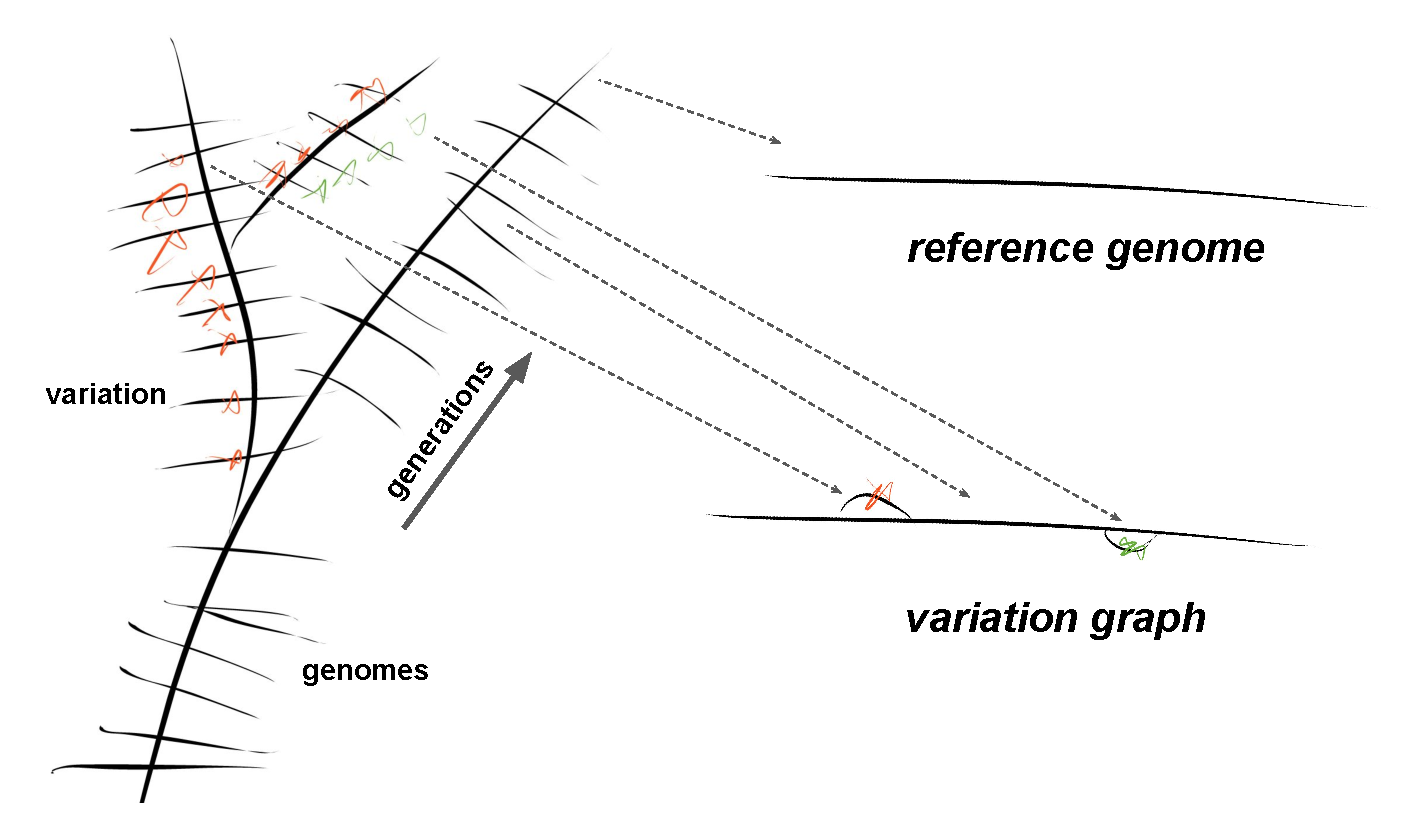
\includegraphics[width=1.0\textwidth]{Chapter1/Figs/phylogeny_and_vg.pdf}
  \caption{
    The tree of life, reference genomes, and variation graphs.
    } 
\label{fig:tree_of_life}.
\end{figure}

Resequencing has arisen in response to the technical properties of the most commonly-used DNA sequencing technologies.
These ``second generation'' sequencing-by-synthesis technologies produce abundant and inexpensive short reads of up to 250 base pairs, and in the past decade have become the largest source of data in the DNA sequencing market.

Higher sequencing costs previously motivated the application of expensive computational approaches to analyze all the sequences of interest simultaneously.
The decades prior to the development of cheap sequencing saw the use of multiple sequence alignment algorithms with high computational complexity.
Analyzing hundreds or thousands of sequences with such techniques is expensive but justifiable given the costs of acquiring them.

However, such approaches became \DIFdelbegin \DIFdel{completely inconceivable }\DIFdelend \DIFaddbegin \DIFadd{too expensive }\DIFaddend as new sequencing technologies allowed the generation of tens and then hundreds of gigabytes of data in a single run.
The new, low-cost techniques allowed joint analyses of thousands of genomes from a single species.
Resequencing provided a practical means to complete these analyses.
\DIFdelbegin \DIFdel{The }\DIFdelend \DIFaddbegin \DIFadd{By relating data to a common linear reference system, the }\DIFaddend alignment phase could be completed independently and in parallel, with each sample compared to the common reference genome\DIFdelbegin \DIFdel{, and only }\DIFdelend \DIFaddbegin \DIFadd{.
Only }\DIFaddend in a final phase of analysis might all the genome data be collected together for the inference of alleles at a given genetic locus.
\DIFdelbegin \DIFdel{By enabling the analysis of genomes at a previously unthinkable scale, resequencing became the core genome inference pattern in genomics.
The standardization of data formats promulgated in large genome sequencing projects supported the separation of different phases of analysis, yielding a rich ecosystem of interacting tools.
}\DIFdelend %DIF > This approach affords scalability to genomic analysis, and has become standard within the field wherever large numbers of samples must be considered.
%DIF > By enabling the analysis of genomes at a previously unthinkable scale, resequencing became the core genome inference pattern in genomics.
%DIF > The standardization of data formats promulgated in large genome sequencing projects supported the separation of different phases of analysis, yielding a rich ecosystem of interacting tools.

In resequencing, the reference sequence shapes the observable space\DIFdelbegin \DIFdel{in a process that is often called }\DIFdelend \DIFaddbegin \DIFadd{, resulting in an effect known as }\DIFaddend \emph{reference bias}.
DNA sequencing reads that contain sequence which is divergent from or not present in the reference sequence are likely to be unmapped or mismapped.
This results in lower coverage for non-reference alleles, in effect forcing new samples to appear more similar to the reference than they actually are.
Divergence itself frustrates the genome inference process, as alignment may produce different descriptions of diverged sequences depending on the relative position of the read.
Alignment works best when the sequences we are aligning are similar to the reference.
Increasing divergence requires greater computational expenditure to overcome reference bias.

We can avoid reference bias by working on pure assemblies generated only from the sequencing data in our experiment and unguided by any prior information.
Doing so can be rigorous, but comes at a significant cost\DIFdelbegin \DIFdel{, especially when the assembly algorithm requires us to load all the sequencing data into memory simultaneously.
We will require much higher coverage to obtain the same level of accuracy in our assembly as we will have when resequencing, and our read lengths will limit the length of contiguous sequences we can infer.
Virtually all assembly algorithms lose information about their source reads through the process of assembly, and this information must be somehow reconstituted if we wish to apply downstream algorithms to the input data in the context of the output of the assembler.
%DIF < No practical algorithm allows us to jointly consider all the samples in a large sequencing experiment in the context of an assembly generated from their reads.
}\DIFdelend \DIFaddbegin \DIFadd{.
Obtaining whole genome }\emph{\DIFadd{de novo}} \DIFadd{assemblies requires greater sequencing an computational costs than resequencing, putting this approach out of reach for many study designs.
}\DIFaddend 

Genome assemblers frequently use a graphical transformation of their inputs that supports algorithm steps used to infer contigs implied by the reads.
These data structures are typically bidirectional graphs in which nodes are labeled by sequences and edges represent observed linkages between sequences.
If constructed from a set of reads that fully cover the genome, it can be shown that such a graph contains the genome which has been sequenced.
In effect, the assembler works to filter the edges from the graph and un-collapse repeats in order to establish a sequence assembly.

In this work I repurpose the assembly graph data model to build a pangenomic reference system.
Assembly graphs are designed to represent the full set of genomic information to which they are applied, so it is natural to use them to develop coherent reference systems for unbiased sequence analysis.
By building a conceptual framework and data structures that enable resequencing against this structure, we can mirror the patterns and workflows that have already been developed for resequencing.
This allows us to retain the benefits of parallel analysis even while we resolve the issue of reference bias.
By recording genomic sequences as paths through this graph I provide anchors for existing annotations and positional systems within the pangenome.
I call these bidirectional sequence graphs with paths \emph{variation graphs}.


\begin{figure}[htbp!]
  \centering
  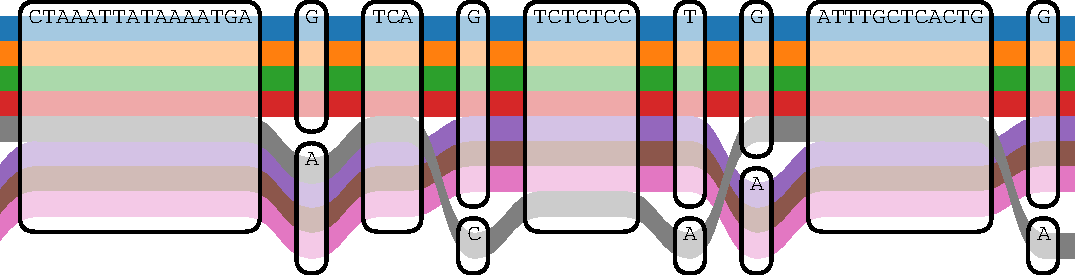
\includegraphics[width=1.0\textwidth]{Chapter1/Figs/vg_tubemap.pdf}
  \caption[A variation graph]{
    A fragment of a variation graph built from fully-assembled \emph{Saccharomyces cerevisiae} genomes.
    Colored paths represent genomes which traverse sequences (nodes).
    Edges are implied by the path structure of the graph.
    The construction and properties of the graph are described in section \ref{sec:yeast_cactus}.
    This visualization was rendered using the SequenceTubeMap \url{https://github.com/vgteam/sequenceTubeMap}.
    } 
\label{fig:variation_graph_tubemap}.
\end{figure}

\DIFdelbegin \DIFdel{In this chapter I will provide background context for my work.
I will cover }\DIFdelend \DIFaddbegin \DIFadd{This chapter provides historical justification for the need for an integrative model for sequence analysis like the variation graph.
I contextualize my work within }\DIFaddend the history of DNA sequencing \DIFdelbegin \DIFdel{methods}\DIFdelend \DIFaddbegin \DIFadd{(\ref{sec:genome_inference})}\DIFaddend , assembly algorithms \DIFdelbegin \DIFdel{, and the development of reference genomes and their use in resequencing.
Finally, I will review similar data models that are used in genome inference.
In the }\DIFdelend \DIFaddbegin \DIFadd{(\ref{sec:genome_assembly}), resequencing methods (\ref{sec:reference_genomes}), and pangenomic models (\ref{sec:pangenomes}).
This deep introduction is meant to justify the need for an integrative model like the variation graph to serve as a coordinating system in a research setting characterized by increasing data scale and complexity.
Readers who need no further introduction to these issues should continue to section \ref{sec:graphical_techinques}, which reviews recent work on algorithms based on data models similar to variation graphs.
}

\DIFadd{The }\DIFaddend remainder of the \DIFdelbegin \DIFdel{work }\DIFdelend \DIFaddbegin \DIFadd{thesis builds on this foundation.
In chapter \ref{chapter:variation_graphs}, }\DIFaddend I describe data structures and algorithms that allow the use of variation graphs as a reference system for unbiased genome inference\DIFdelbegin \DIFdel{, and }\DIFdelend \DIFaddbegin \DIFadd{.
Finally, in chapter \ref{chapter:applications}, I }\DIFaddend demonstrate the benefits of this approach with a series of \DIFdelbegin \DIFdel{experiments}\DIFdelend \DIFaddbegin \DIFadd{experimental case studies}\DIFaddend .

\section{Genome inference}
\DIFaddbegin \label{sec:genome_inference}
\DIFaddend 

% What do we mean by genome inference
% half page
Not two centuries have passed since the first experiments that demonstrated the existence of genetic material \cite{mendel1866versuche}.
In the first part of the twentieth century, these ideas about heredity grew into the core of a modern synthesis linking biological micro- and macro-evolutionary theory to the quantitative basis of genetics \cite{huxley1942evolution}.
It was understood that DNA encoded the information that gave rise to biological structures \cite{avery1944studies}.
The discovery of the structure of DNA in the 1950s \cite{watson1953molecular} made clear the nature of that information and the mechanism for its faithful transmission from generation to generation.
This knowledge, coupled with the sequencing and synthesis of proteins, which demonstrated that they had distinct polymeric chemical identities \cite{sanger1951amino} led to Crick's postulation of the ``central dogma'' of biology \cite{crick1958protein,crick1970central}.
Simply stated, the ``dogma'' argues that in living systems' information is transcribed from DNA to RNA and ultimately translated into proteins, which guide and structure the cell and thus living organisms.
The central dogma clarifies the significance of the sequence of the genome, and over the following decades a series of projects scaled up the throughput and fidelity of DNA sequencing until \emph{genome inference} became a practical and everyday reality in biology.

\subsection{Reading DNA}
% Genome sequencing techniques
% half page

The quest to sequence genomes began with arduous and sometimes dangerously radioactive experimental techniques, in which years of researcher time could be spent in obtaining sequences of tens of bases from partly-characterized sources.
It has then progressed through three distinct phases.
In the first, these early laboratory techniques gave way to automated sequencing using chain terminator chemistry, and related techniques were ultimately used to generate genome sequences for human and a number of organisms, albeit at high costs.
In the second phase, \emph{multiplex} sequencing reactions were used to miniaturize the chain terminator reaction and observe its progression using fluorescent imaging or electrical sensing, evoking a drop in cost per sequenced base of many orders of magnitude, and simplifying library preparation steps dramatically by sequencing clones of individual molecules.
The third wave of development has been characterized by two techniques which allow realtime observation of single DNA molecules.
These produce enormously long read lengths that are limited by the molecular weight of input DNA, but produce readouts with high per-base error rates.
Supporting the second and third wave are methods that allow for haplotype-specific sequencing and the observation of long range structures in the genome.

\subsubsection{The old school}
% Sanger sequencing, BACs, etc.

In the 1970s a group led by Walter Fiers published the first complete gene \cite{jou1972nucleotide}, and then genome sequence \cite{fiers1976complete} from the MS2 bacteriophage using laborious digestion and 2-dimensional gel electrophoresis techniques to sequence RNA based on work by Fredrick Sanger and colleagues \cite{sanger1965two, adams1969nucleotide}.
To avoid the limitations of digestion based assays, Ray Wu and colleagues developed a sequencing technique based on the partial blockage of DNA polymerization with radiolabeled nucleotides \cite{wu1972nucleotide, padmanabhan1974chemical}.
Subsequently, Sanger developed a reliable DNA sequencing method based on the same DNA polymerization chain-termination concept by dividing the sequencing reaction into four, one for each base, and sorting the resulting DNA fragments in parallel on an acrylamide gel \cite{sanger1977dna}.
Optimized and implemented using fluorescent chemistry \cite{strauss1986specific}, this approach, now known as Sanger sequencing, became the foundation of the first commercial sequencing machines in the late 1980s.

Sanger sequencing was the workhorse standard of biology for nearly 30 years, from the late 1970s until the mid 2000s.
Its read length is limited by the reaction efficiency required to obtain a fraction of terminations at every base in the sequence.
In practice, reads of 500 to 1000 base pairs can be obtained.
With clonal DNA as input the per base accuracy of the method is extremely high, as each base readout reflects the termination of large numbers of molecules \cite{castiblanco2013primer}, a feature which has ensured it remains important for validation of sequencing results \cite{sikkema2013targeted}.
However, heterogeneity in the input DNA library can produce muddled signals that rapidly become uninterpretable.
Insertions and deletions (indels) will cause a loss of phase in the sequencing trace \cite{tenney2007tale}, a problem which is still encouraging algorithm development \cite{hill2014poly}.
In order to sequence whole genomes, which are often heterozygous, laboratory techniques were developed to allow the segregation of clonal DNA as a substrate for sequencing.
These include bacterial artificial chromosomes (BACs) and their equivalent in yeast (YACs) \cite{monaco1994yacs}.
The effective read length could be increased by using ``mate pair'' techniques, in which the ends of a longer molecule would be sequenced \cite{schmitt1996framework}.
To yield fully assembled genomes, these data required the development of suitable computational techniques \cite{myers2000whole}.

\subsubsection{``Next generation'' sequencing}

In the late 1990s and early 2000s, several groups began exploring alternative sequencing strategies.
In the ultimately dominant one, DNA that has been clonally arrayed on a surface is directly sequenced using fluorescent imaging.
Sequencing progresses through the synthesis of the second strand of each of the molecules, and so these techniques are typically called ``sequencing-by-synthesis.''
This modality allowed for a massive parallelization of the sequencing reaction, and has resulted in a dramatic reduction of cost.

In 2003 George Church and colleagues demonstrated that individual sequences could be read from polymerase colonies or ``polonies'' suspended in an acrylamide gel using fluorescence microscopy \cite{mitra2003fluorescent}.
This fluorescent imaging model became the basis for ``next generation'' sequencing \cite{shendure2008next}.
Contemporaneously, a sequencing-by-synthesis method which is now known as Illumina dye sequencing, was implemented using laser fluorescent imaging and reversible terminator technology developed by Shankar Balasubramanian and David Klenerman at Solexa (later acquired by Illumina) \cite{balasubramanian2004arrayed, bentley2008accurate}.
Rather than polymerase colonies embedded in an emulsion or gel, Solexa's technology relied on ``bridging PCR'', in which the polymerized clones of a particular fragment were locally hybridized to an adapter-bearing surface of a flowcell.
Controlled synthesis of the second strand, based on reversible terminator chemistry \cite{canard1994dna} and fluorescently labeled dNTPs, is then used to observe the sequence of the DNA molecule in each colony.

A diverse set of similar approaches were explored during this period, although few saw more than limited success in the sequencing market.
Church's group focused on a hybridization based sequencing protocol proceeded by an emulsion based polony PCR step \cite{shendure2005accurate}, and later attempted to commercialize an open source sequencing device (the Polonator)\footnote{My interest in open source projects, developed while an undergraduate studying the social sciences, led me to work on this device. The project introduced me to biology, bioinformatics, and DNA sequencing, which have attracted my interest and effort ever since.}.
In ion semiconductor sequencing direct observation of pH changes were used to determine DNA sequences \cite{rusk2010torrents}.
454 Life Sciences' ``pyrosequencing'' implementation used a luciferase reporter assay to track the progression of DNA synthesis \cite{margulies2005genome}, and it was used to generate the first whole genome human sequence using ``next generation'' techniques \cite{wheeler2008complete}.
Helicos commercialized the first single-molecule sequencing system, using a similar chemistry to Illumina's but observing single molecules rather than pools, which proved technically challenging and only saw use in its own development \cite{harris2008single}.

Illumina's sequencing protocol provides greater throughput and a superior error profile relative to these methods.
Its low per base error rates and handful of context specific error types simplify analysis \cite{allhoff2013discovering}.
It is unsurprising that the vast majority of sequencing data produced in the 2010s comes from Illumina sequencers.
Illumina's sequencing technology is characterized by short reads (<250bp) with per-base accuracy ($\approx 99.5\%$) comparable to that of Sanger sequencing.
Although the read length has been increased by optimization of the technology, the difficulty of achieving perfect per-base reaction efficiency apparently prevents greater extension of the read length.

A number of methods extend the genome inference capacity of Illumina sequencing, allowing it to be used to infer long haplotypes and genome organization.
Moleculo, and later 10X Genomics commercialized barcode-guided haplotype sequencing and assembly \cite{zheng2016haplotyping}.
The later has focused on providing raw tag information that could be used downstream by an array of haplotype-resolution and assembly tools \cite{mostovoy2016hybrid}.
The single template aspect of Illumina paired end sequencing allows longer contiguous DNA reads to be obtained by merging partly-overlapping read pairs computationally \cite{magovc2011flash}.
Single-cell DNA template strand sequencing (strand-seq) can be used to obtain reads from only one half of the chromatids in a single cell \cite{falconer2012dna} via bromodeoxyuridine (BrdU) treatment and cleavage of the nascent strand, which can aid in haplotype reconstruction \cite{porubsky2016direct}.
The Hi-C method \cite{lieberman2009comprehensive} uses bisulfite treatment to generate read pairs that are likely to physically co-locate \emph{in vivo}, thus enabling the mapping of long range DNA and chromatin interactions.
It may be combined with other sequencing information to obtain estimates of the syntenic ordering of contigs produced by assembly \cite{ghurye2018integrating}, which has already been used to obtain \emph{de novo} reference quality genomes in several difficult sequencing projects including amaranth \cite{lightfoot2017single}, \emph{Aedes aegypti} \cite{dudchenko2017novo}, and the domestic goat \cite{bickhart2017single}.

\subsubsection{Single molecules}

All previously described sequencing techniques are dependent on the observation of pools of molecules.
These methods benefit from amplification of DNA, which increases signal, but also adds and a potential source of error to DNA sequencing.
They also suffer from de-phasing resulting from imperfect stepwise reaction efficiency, which fundamentally limit the maximum length of an accurate read.
A method to sequence single molecules accurately would theoretically allow longer read lengths, but this requires the difficult, direct observation of DNA.
Efforts to develop such a method have been continuously underway throughout 2000s and 2010s.
Two successful commercial sequencing platforms based on this principle are rapidly defining a new technical phase of genome inference.

By utilizing zero-mode waveguides (ZMWs) to observe DNA polymerase in real time, Pacific Biosciences (PacBio) generated the first successful commercial single-molecule sequencing system \cite{eid2009real}.
In this platform, DNA polymerase is immobilized in sub-diffraction size, picoliter detection volumes at the bottom of wells formed in aluminum on a glass slide \cite{korlach2008selective}.
Single stranded DNA and fluorescently-labeled dNTPs are added to the buffer above the ZMWs.
As synthesis progresses, the fluorophore attached to the DNA base that is being incorporated will tend to remain inside the ZMW longer than would be expected due to random diffusion of the dNTPs, allowing a readout of the sequence of incorporated bases as a series of fluorescent pulses.
The base-level error rate of sequencing is high, up to 15\%.
It is difficult to perfectly observe the series of fluorophores pulled into the well, and random occupancy is often indistinguishable from polymerization-mediated occupancy, which results in insertion errors.
Although subtle context dependent biases do exist \cite{ono2012pbsim}, due to their genesis in Brownian motion, the errors themselves may be considered as almost perfectly random in analysis \cite{ross2013characterizing,myers2014efficient}.
In recent years PacBio's system has become a foundational technology in genome sequencing, with many recent genome assemblies completed using it \cite{rhoads2015pacbio}.

The idea that electrophoresis of DNA through nanometer scale pores might allow the direct sequencing of DNA was first postulated in the late 1980s by David Deamer and others \cite{deamer2016three}.
While the sequencing model itself is among the simplest ever proposed, it would take twenty-five years of work \cite{kasianowicz1996characterization,purnell2008nucleotide} before the technique was brought to market by Oxford Nanopore (ONT) \cite{mikheyev2014first} and used to fully sequence genomes \cite{loman2015complete, jain2018nanopore}.
In this approach, a DNA strand is pulled through a nanometer pore by electrophoresis.
The specific DNA bases in the pore effect characteristic changes in the electric current density, and the DNA molecule can be read by measuring the changes in current over time.
Due to context and history-dependent effects that distort the signal, the measured patterns in the current flux must be interpreted by sophisticated models that have been trained to convert the traces to DNA sequences \cite{david2016nanocall}.
As with PacBio, its per-base error rate approaches 15\%.
In practice nanopore sequencing has the highest error rate of any commercially available method, which reflects the difficulty of mapping between the observed signal and the underlying DNA sequence.
Nanopore sequencing can also obtain the longest reads of any sequencing technology, with megabase-scale reads reported by some users.

%, single molecule ONT/PacBio (3rd gen)

\subsection{Genome assembly}
\label{sec:genome_assembly}

Due to technical limits that are unlikely to ever be fully eliminated, individual DNA sequence reads are rarely able to cover the entire genome of an organism.
This means that in many cases, the best sequencing data possible is a set of random reads sampled from fragments of the genome. 
In whole genome ``shotgun'' sequencing the genome is fragmented, perhaps by sonication or enzymatic digestion, and the resulting fragments are sequenced and then reassembled using computer programs \cite{gardner1981complete, sanger1982nucleotide}.
This process necessitates a reconstructive step in which the information obtained from the sequenced fragments is reassembled into the whole genome from which they arose.
This process is known as \emph{assembly}, and computer algorithms implementing it have been used when inferring genome sequences since the generation of the first whole genome sequence for bacteriophage $\varphi$X174 in 1977 \cite{sanger1977nucleotide, staden1979strategy}.

The earliest assembly algorithms have come to be known as ``overlap-layout-consensus'' (OLC) algorithms, due to their three-phase strategy.
They first establish a set of head to tail overlaps between reads (overlap), an $\approx O(N^{2})$ order problem when all pairwise relationships are considered between $N$ sequence reads.
However, given an efficient method to find read pairs that are very likely to match together, the overlap step remains tractable as the overall complexity of matching can be reduced to be approximately quadratic in read depth and linear in genome size \cite{huang1992contig}.
These overlaps are then used to establish an estimate of the ordering of the reads (layout).
The layout is then used to generate a consensus sequence through heuristics or dynamic programming over the layout \cite{kececioglu1995combinatorial}.
This final phase is equivalent to the multiple sequence alignment (MSA) problem, although instead of generating an MSA as output methods would typically take the consensus sequence, as the objective is often to reconstruct a linear representation of the input genome.
Early assemblers committed frequent assembly errors, which necessitated time-consuming manual ``finishing'' \cite{gordon1998consed}.
The OLC assembly approach was utilized by genome projects for the following twenty-five years, including in the public Human Genome Project (HGP), where BAC clones of 150kb fragments of the genome were sequenced, initially assembled by algorithm and finally manually finished into the ``golden path'' that would become the reference genome \cite{international2001initial}.

In principle, the assembly process could be fully automated, but as late as the early 1990s this frequently was not seen as feasible due to the lack of reliable algorithms \cite{mahy1991sequencing}.
The improvement of OLC algorithms eventually met the challenge, yielding methods such as PHRAP \cite{green1999phrap} (a quality aware assembler that saw extensive use downstream of Sanger sequencers), TIGR \cite{sutton1995tigr} (which was used in the generation of the first assembly of a free living organism, the 1.8Mbp genome of \emph{Haemophilus influenzae} \cite{fleischmann1995whole}), GigAssembler \cite{kent2001assembly} (which was used by the HGP), and the Celera assembler \cite{myers2000whole,miller2008aggressive} (which saw extensive use in the generation of early large whole genome assemblies in the late 1990s and early 2000s, including the privately funded genome project \cite{venter2001sequence}\footnote{This project apparently still relied on data produced by the HGP \cite{waterston2002sequencing}, but the significance of this reliance was disputed by researchers involved in the private project \cite{myers2002sequencing}, who argued that the manner in which they used the public sequences avoided contamination by manual finishing done by the HGP.}.)
The process implemented in the Celera assembler (including repeat masking) has remained essential to the genome assembly problem until the present.

In 2005, Myers formalized an idealized version of the assembly problem in the \emph{string graph} data structure \cite{myers2005fragment}, which is a sequence graph induced from the overlaps in a set of shotgun sequencing reads.
This model demonstrates that repeats greater than the length of a sequence read will collapse into single copies in the graph, while unique sequences will form loops between different repeat classes that flank them.
The string graph can be shown to represent the full information available in the input sequence data, and successful assembly algorithms are built around an induction of the string graph via the construction of the FM-index \cite{ferragina2001experimental} from Illumina read sets \cite{simpson2010,simpson2012efficient,li2015fermikit}.
If not using compressed data structures and low-error reads, the repeats are often irresolvable and may be masked from the assembly process to improve performance on the tractable non-repetitive regions of the genome, which is a strategy still promoted and employed by Myers \cite{myers2014efficient}.
Canu and FALCON, which to some extent stand as contemporary implementations of the Celera assembly process, are among the best-performing assemblers for noisy single-molecule sequencing data that is the mainstay of current genome assembly projects \cite{chin2016phased,koren2017canu}.
These and similar methods have shown that long reads can be used to fully assemble genomes without human finishing \cite{loman2015complete,jain2018nanopore}.

The repeat problem has been tackled in various ways, but one of the most enduring solutions resolves the issue through the reduction of the assembly overlap graph to a de Bruijn graph (DBG) \cite{pevzner2001eulerian}.
In this approach, the read set is fragmented into all subsequences of reads of a given length $k$, and a graph is constructed where $k$-mers label nodes and overlaps of $k-1$ between successive $k$-mers induce edges representing linkages between them.
The de Bruijn graph simplifies the representation of the read set, providing a clean basis for assembly algorithms.
It enabled the first \cite{zerbino2008velvet,simpson2009abyss,iqbal2012novo}, and most memory-efficient assembly methods for short read sequencing data, with techniques like bloom filters \cite{chikhi2013space}, succinct DBGs \cite{bowe2012succinct,li2015megahit}, and minimizer partitioning \cite{chikhi2016compacting} applied to generate a compressed representation of the graph.
DBG based assemblies suffer from the loss of information induced through the $k$-merization of their input, causing a reduction in assembly contiguity \cite{earl2011assemblathon}, although in practice this can be mitigated by reconsideration of the input reads and read pairs \cite{butler2008allpaths}.
They also are applicable only where the sequence error rate is low enough for overlapping reads to be expected to have exact matching $k$-mers of the appropriate size (typically, $k \in [20 \ldots 50]$ base pairs), and as such cannot be applied to third generation single molecule sequencing due to its inherently high error rate.

Many of the sequencing methods I have described above are still in use today.
Each popular method, as it fades from use, remains relevant in a niche area where its particular properties provide it a comparative advantage.
As a result, we are not presented today with a single ideal sequencing method, but a menagerie of approaches, each with its own limitations and benefits, and current assembly pipelines require thoughtful design to incorporate these myriad sources of information.
It would appear that in order to use these many technologies to generate the best-possible assemblies we must bring them together in a single model \cite{chaisson2018multi}.
A current development in assembly focuses on the design of a common interchange format for which to organize such assembly processes, which has been implemented as the GFA v1 and v2 formats.\footnote{\url{https://github.com/GFA-spec/GFA-spec}}
This file format and the data model it implies is an essential link between the work that I present later in this thesis and the problem of genome inference.

\section{Reference genomes}
\DIFaddbegin \label{sec:reference_genomes}
\DIFaddend 

Obtaining a single genome sequence \emph{de novo} is an arduous task, and remains a complex problem.
The result is a valuable object which can be used to lower the cost of subsequent analyses and enable direct whole genome comparisons which provide a full perspective on the genetic relationship between multiple individuals or species.
The need for reference genomes is clear, and they are collected in open public databases to allow their dissemination and use by researchers.
NCBI's RefSeq release 89 of July 13, 2018 contains some 81,345 organisms\footnote{\url{https://www.ncbi.nlm.nih.gov/refseq/}}, although it should be noted that only a small fraction of these genomes are eukaryotic.
Recent developments in long read, single molecule sequencing have enabled great decreases in the cost and complexity of generating high-quality genome assemblies, supporting a recent project to generate reference quality genomes of ten thousand vertebrates \cite{genome2009genome,koepfli2015genome}.

The reference genome serves as an anchor for annotations that describe sequences and regions of interest within the genome, such as genes, exons, chromatin structures, DNA interacting proteins, and genetic variation \cite{sherry2001dbsnp,quinlan2010bedtools,encode2012integrated}.
An established reference genome can serve as a conceptual foundation for the communication and interpretation of scientific results \cite{kent2002human}, and is seen as essential for collaboration and the development of a genome research community in a particular organism \cite{smith1998functional,cherry1998sgd}.

Reference genomes tend to represent only a single version of each genomic locus.
This conceptual simplicity is a core feature of their public use.
Although the issue of genetic diversity has always been appreciated by those who work with genomes, expediency has encouraged the use of linear models for reference genomes.
Within the HGP, members of the consortium could observe diversity within the BAC clones that they had sequenced from different human donors, and initiated a debate about the inclusion of heterozygosity in the reference itself.
Ultimately, a graphical model was seen as too complicated, and practicality necessitated the publication of a linear reference based around what came to be called the ``golden path'' through the assembly\footnote{Personal communication with David Haussler.}.
Since early releases, the human reference genome has included alternative versions of some regions, with current releases including alternates for around 200 loci \cite{schneider2017evaluation,church2018genomes}, but these are represented as linear sequences without a unifying alignment between them, which complicates their use in resequencing and annotation \cite{jager2016alternate}.

% history of reference sequences
% use of the reference sequence in analysis
\subsection{Resequencing}
\DIFaddbegin \label{sec:resequencing}
\DIFaddend 

Due to the high cost of obtaining error-free, full length genomes, standard practice will use the best genome assembly for a given organism as a \emph{reference genome} when analyzing the sequences of other organisms from the same species.
To do so, the genomes of the other individuals do not need to be fully assembled, and instead shotgun sequencing libraries from these new individuals may be aligned back to the reference to find small differences between the genomes.
To distinguish it from whole genome sequencing and assembly, this process is known as \emph{re}sequencing.

Resequencing has two phases.
In the first phase, reads from the sample or samples under study are aligned against an appropriate, genetically similar, reference genome.
In the second phase, the aligned reads (alignments) are processed together locus by locus to determine allelic variation within the samples relative to the reference genome.

\subsection{Sequence alignment}
\label{sec:sequence_alignment}

An \emph{alignment} expresses one sequence in terms of a set of positions, edits, and matches to another.
Algorithms to determine the most plausible alignment between a pair of sequences have as long a history as sequencing itself.
The first significant attempts to algorithmically assess sequence homology and divergence between protein sequences arose in the 1960s with Fitch's method for homology detection \cite{fitch1966improved}.
To account for insertions and deletions, this method required the comparison of many subsequences of two sequences to be compared, resulting in poor computational bounds.
In 1970, Needleman and Wunsch responded with an O(NM) time algorithm for the global alignment of sequences \cite{needleman1970general}.
Given strings to compare of length $N$ and $M$, the algorithm builds an $M \times N$ matrix in which any possible full length alignment between both sequences can be expressed as a path through a series of cells.
The matrix is designed such that a match corresponds to the shortest (diagonal) path through the matrix, and insertions and deletions correspond to horizontal or vertical movements.
To determine the most-likely path, Needleman and Wunsch apply a recurrence relation dependent on the characters at each pair of positions in the strings and the values of the cells above and/or to the left.
This implements a dynamic programming (DP) method \cite{bellman1952theory}.
For each cell, the score is given as the maximum of: the score of cell to the diagonal plus a bonus if the corresponding sequence characters are the same and minus a penalty if they are different; and the scores of the cells above and below minus a penalty corresponding to the weight given to an insertion or deletion.
Finally, we determine the optimal path beginning from the opposite extreme cell of the matrix from where the scoring began, in which we walk back through the successive maximum scores until reaching the opposite extreme corner of the matrix.
This ``traceback'' encodes the alignment, which is most-simply represented as a vector of pairs of matched bases in each sequence.
It can be shown that provided full evaluation of the dynamic programming problem, the optimal alignment is obtained given a set of scores parameterizing the recurrence relation.

This alignment algorithm is known as a ``global'' alignment algorithm, in that the alignment covers all bases of both sequences.
In practice, this type of comparison is not always needed, and it can be advantageous to obtain only the optimal sub alignments between sequences.
Smith and Waterman provided a clean modification of the algorithm of Needleman and Wunsch, altering it to prevent negative scores, which allowed it to produce optimal ``local'' alignments \cite{smith1981comparison}, while ignoring regions unlikely to contain significant homology.
The algorithm, further refined by Gotoh \cite{gotoh1982improved} to enable affine gaps\footnote{In affine gap schemes the cost of a gap per base decreases as its length increases. Such a scheme approximates the $\zeta$-distributed excursions of a particle under Brownian motion, which structure the length of insertions and deletion mutations observed in nature.} and computation in $O(MN)$ time, is today one of the most important in genome analysis.
The amount of work on this topic is considerable, and the subsequent decade yielded numerous modifications of the basic alignment concept, for instance reducing the memory bounds to $O(N)$ through a divide and conquer approach \cite{myers1988optimal}, and further explorations of affine gap scoring schemes \cite{altschul1986optimal,gotoh1990optimal}.
Subsequent works have offered improved implementations, using vectorized instructions to improve the runtime of the algorithm \cite{farrar2007striped} and heuristics to selectively evaluate only part of the DP matrix \cite{suzuki2017acceleration}.
However, such changes were not sufficient to enable alignment against large sequence databases.

$O(MN)$ algorithms for sequence alignment are impractical when either $M$ or $N$ becomes large.
Naturally, as sequence databases grew and the size of sequenced genomes increased, heuristic strategies to efficiently reduce the alignment problem size were introduced.
When aligning a short sequence against a large database we expect to obtain a sensitive alignment, but provided sufficient homology between the sequence and the database it is unlikely that we need to evaluate the full problem using an algorithm like Smith-Waterman-Gotoh (SWG).
By indexing either the query or target set of sequences to efficiently obtain patterns of exact matches, candidate sub-regions of both can be isolated and submitted for more sensitive alignment.

This strategy was implemented in the mid- to late-1980s in the FASTA \cite{pearson1988improved} and BLAST \cite{altschul1990basic} alignment algorithms.
FASTA first uses a seeding step that finds exact matches between the query and target, using chains of short $k$-mer seeds to establish the longest matching subsequences.
A few of the best scoring candidates are enumerated and evaluated using a banded SWG algorithm.
In contrast, BLAST implements a fully heuristic alignment process based solely on the $k$-mer seeds and ungapped alignment.
This is much faster than FASTA but can perform slightly worse with highly divergent sequences.
BLAST's heuristic alignment is many orders of magnitude faster than full DP based algorithms at a minor cost to accuracy.
The popularity of BLAST in biology\footnote{The BLAST1 paper has been cited more than 70,000 times as of August 2018.} is clear evidence of the importance of the alignment problem to all kinds of genomic analysis.
It is also evidence that minor losses in accuracy are acceptable given the cost of sequence analysis in large data sets.
Jim Kent's Blast-like alignment tool (BLAT) indexes the target set with non-overlapping $k$-mers and queries all $k$-mers in the reads, yielding a method that is less sensitive but several orders of magnitude faster again than BLAST \cite{kent2002blat}.

As reliable commercial second-generation sequencing systems became available the rate of sequence data acquisition growth rapidly outstripped the rate of improvement in computing performance \cite{leinonen2010sequence,kodama2011sequence}.
This necessitated further improvements in the computational cost of sequence alignment.
The most-widely used of these methods focused on the increasingly prevalent problem of aligning short reads to reference genome type sequence databases.
Due to the high quality of the reference sequence, low error rate of the short ($\leq$100bp) reads, and low nucleotide diversity of humans (where $\theta \approx 10^{-3}$), algorithms that focused on exact string matching had great success.
Much like BLAST and BLAT, the first wave of aligners capable of indexing the human reference genome and aligning short reads to it utilized exact $k$-mer matching via hash tables followed by local alignment \cite{li2008soap,lee2014mosaik,li2008mapping}.
Substantial improvements would be yielded by the development of aligners based on contemporary developments in compressed data structures.

\DIFaddbegin \subsubsection{\DIFadd{Compressed full text indexes}}
\label{sec:compressed_full_text_indexes}

\DIFaddend The suffix tree \cite{weiner1973linear} encodes all suffixes of a sequence $S$ in the structure of a tree such that the suffixes may be enumerated by a depth first search (DFS) of the tree.
This structure can be used to determine if a given sequence $q = c_{1}c_{2}\ldots c_{|q|}$ is present in $S$ in $O(|q|)$ time.
Search begins at the root, progressing across the topology (edge or node) of the tree which is labeled with the next character until no further matches may be found.
By labeling the tree with the sequence positions corresponding to each node, the search may also yield the positions of the exact matches detected within $S$.
Suffix trees may be built in linear time and space relative to their input \cite{ukkonen1995line}, and support diverse algorithms for string comparison \cite{apostolico1985myriad}, such as whole genome alignment \cite{delcher1999alignment}, but they require relatively large amounts of memory per input base.
They were superseded by equivalent data structures with better memory bounds such as the suffix array\DIFdelbegin \DIFdel{(}\DIFdelend \DIFaddbegin \DIFadd{, }\DIFaddend which represents the \DIFdelbegin \DIFdel{tree in a linear array of suffix sort ranks) }\DIFdelend \DIFaddbegin \DIFadd{lexicographically ordered suffixes as a vector of numbers }\DIFaddend \cite{manber1993suffix}, and its compressible sibling the Burrows-Wheeler Transform (BWT) \cite{burrows1994block}.
\DIFdelbegin %DIFDELCMD < 

%DIFDELCMD < %%%
\DIFdel{By augmenting the BWT to enable the exact matching via emulation of the suffix tree, Paolo Ferragina and Giovanni Manzini developed the FM-index \mbox{%DIFAUXCMD
\cite{ferragina2000opportunistic,ferragina2004alphabet}}\hspace{0pt}%DIFAUXCMD
.
Given a string $S$, }\DIFdelend \DIFaddbegin \DIFadd{Compressed suffix arrays (CSA) (equivalently, }\DIFaddend the \DIFaddbegin \DIFadd{``fast, minute'' }\DIFaddend FM-index\DIFdelbegin \DIFdel{may be built using a series of transformations and auxiliary data structures that induce the suffix tree by constructing the BWT.
First, we add marker characters for the start and end with lexicographic order less and greater than the rest of the characters in the alphabet, e.g. $\#S\$$.
Conceptually, we take all rotations of the sequence and sort them, yielding matrix $M$, which is sometimes called the Burrows-Wheeler Matrix (BWM), but in fact this is done in a space-efficient manner without the enumeration of the rotations.
This sort has many similarities to the suffix tree, and for instance it can be seen that a lexicographically-ordered DFS through the suffix tree would enumerate the prefixes of the rotations of the sequence preceding the terminal character $\#$ in the same order as they are sorted.
The suffix array $SA$ is given by the vector of the suffix ranks in the sorted order they occur in $M$, and is related to the ordering of characters in the first column $F$, while the BWT is given as the last column, $L$.
If the input text has repetitive patterns, then these will tend to result in runs in the BWT that may be compressed using various schemes.
To emulate traversal of the suffix tree, it is sufficient to construct a function $LF(i)$ which maps between indexes $L[i] = F[j]$ which represent the same character.
This is done by the augmentation of the data structure with array $C$ such that $C[c]$ returns the number of characters in the text that are lexicographically smaller than $c$, and a function $rank(c,k)$ that yields the number of instances of $c$ in the prefix $L[1 \ldots k]$.
Now, $LF(i)$ may be defined as $C[L[i]] + rank(L[i], i)$.
By allowing the traversal of equivalencies between the suffix array and the BWT, $LF$ mapping enables ``backward search''.
Because rotations of $S$ have been ordered in $M$, a given pattern will occur as the prefix of a particular contiguous range of $M$.
We can find all occurrences of a given pattern by maintaining a range }\DIFdelend \DIFaddbegin \DIFadd{) are data structures which combine a compressed representation of the BWT with auxiliary data structures that support rank and select operations on it \mbox{%DIFAUXCMD
\cite{ferragina2000opportunistic,ferragina2004alphabet,grossi2005compressed}}\hspace{0pt}%DIFAUXCMD
.
To support suffix array operations in this compressed context, including pattern matching and positional queries, standard implementations include additional auxiliary information, in particular a sampled subset of the entries }\DIFaddend in the suffix array\DIFdelbegin \DIFdel{within which a given pattern occurs, beginning at $s$ and ending at $e$, which we initially set as $s=0$ and $e=|L|-1$.
To search for a pattern, we obtain $s' = C[c] + rank(s,c) + 1$ and $e' = C[c] + rank(e,c)$, walking backwards through the characters $c$ in our query $q$.
Our search terminates when we complete our query or $e' - s' \leq 0$, which indicates that the previous step in the search did not match our target $S$.
The various matches of $q$ in $S$ may now be obtained by the positions in $SA[s \ldots e]$.
The addition of the longest common prefix (LCP) array on the sorted suffixes can be used to emulate all algorithms on suffix trees in this context \mbox{%DIFAUXCMD
\cite{abouelhoda2004replacing}}\hspace{0pt}%DIFAUXCMD
, and in turn this enables $O(|q|)$ search of queries against $S$.
Of particular relevance to this work, when completing a phase of backward search we could use the LCP to traverse the suffix links in the suffix tree and continue with the next (partially overlapping) maximal exact match}\DIFdelend \DIFaddbegin \DIFadd{.
See section \ref{sec:fmidx_csa} for a detailed review of the important features of these data structures as they relate to string matching}\DIFaddend .

The FM-index is used in modern short-read aligners such as BWA \cite{li2009fast} and BOWTIE \cite{langmead2009ultrafast}, which used backtracking LF alignment to directly align sequences to the suffix array encoded in the FM-index.
This backtracking search is fast, but has problems detecting indels (as these require exponentially more backtracks to infer) and performs less well with increasing read length.
In response, the authors merged initial exact matching with a final DP step to yield ``long read'' capable aligners like BWA-SW \cite{li2010fast} and BOWTIE2 \cite{langmead2012fast}.
Further refinements of this concept yielded BWA MEM \cite{li2013aligning}, which uses a heuristic algorithm to determine ``supermaximal exact matches'' (SMEMs) and reseed ``sub matches'' within them using a bidirectional FM-index (the FMD index).
Due to its relative robustness to error and variation, the MEM concept has ultimately prevailed and as of the time of this writing BWA MEM can be seen as the industry standard method for aligning short reads to the genome.

Much of the second generation sequencing data has been generated for humans in medically-motivated genome wide association studies \cite{uk10k2015uk10k} or population survey projects like the 1000 Genomes Project (1000GP) \cite{1000Gphase1,1000g2015}. % TODO not sure about this phrasing
The development of these methods was accelerated by an open, competitive spirit fostered during the 1000GP, whose primary sequencing data remains the largest completely publicly available data set, with more than 100TB of sequence data available for download from public URLs without any authentication.
There, project participants formalized the resequencing process by generating a series of data formats linking the various stages of analysis, including the sequence alignment/map format (SAM) and its binary equivalent (BAM) \cite{li2009sequence} that is the standard output format for contemporary aligners.


\subsection{Variant calling}

DNA sequencing reads of all types contain errors, and genomes contain diversity.
To resolve these errors and infer the genome's state, we aggregate information from many reads mapping to each locus.
In the context of resequencing, this process is known as \emph{variant calling}.
The simplest methods resemble the consensus step in OLC assembly, and are implemented as heuristic filters on the mutually gapped alignment matrix of a set of homologous sequence reads \cite{koboldt2009varscan}.
A Bayesian model can incorporate prior expectations about the genomic state with the available data to generate a posterior estimate of the probability of polymorphism that can propagate uncertainty to downstream analyses.
It can use first principles to integrate various sources of information in addition to the sequence of the reads themselves, including the base quality (BQ), or machine-estimated probability of an erroneous base call, and mapping quality (MQ), which represents the aligner's estimate that the given alignment is a mismapping or ambiguous \cite{li2011statistical}.
A Bayesian approach also supports the joint analysis of many individuals from the same population.
For instance, in a panmictic population under neutral selection the pattern of observed genotypes should be consistent with Hardy-Weinberg Equilibrium (HWE), and to have confidence in a given genotyping call, the evidence for variation should be stronger than the prior odds of there being no genetic variation at the site.

The earliest implementations of Bayesian variant calling and genotyping were applied to expressed sequence transcripts (ESTs) \cite{marth1999general}.
Competition fostered by the 1000GP encouraged the development of variant calling algorithms based on a variety of principles.
The simplest methods would detect variation given pointwise SNP and indel descriptions directly from the alignments \cite{li2009sequence,depristo2011framework}.
However, this technique was shown to be susceptible to inconsistencies in the alignment process, and several groups developed methods that would reevaluate the alignments in a reference-independent manner in order to homogenize the representation of small variation.
These techniques became known as ``local assembly'' variant detection algorithms, and include the windowed haplotype detection implemented in freebayes \cite{garrison2012haplotype} as well as full local \emph{de novo} assembly based on de Bruijn graphs as implemented in Dindel \cite{albers2010dindel}, Platypus \cite{rimmer2014integrating} and the GATK's HaplotypeCaller.
In parallel, several whole genome \emph{de novo} assembly methods, including SGA and Cortex, were applied to the full data set, yielding variant calls that minimized bias towards the reference genome.
The final project results were merged into a population genome assembly using statistical phasing algorithms \cite{browning2007,howie2011,delaneau2012} guided by genotyping results from sequencing and genotyping arrays \cite{1000g2015}.
Members of the 1000GP also developed a file format for describing collections of resequenced genomes, including their genotypes and inferred haplotypes, the variant call format (VCF) \cite{danecek2011variant}, which has become the standard interchange format for sequencing-based variant and genotyping information.

Due to the absence of a reliable truth set, early variant calling method implemented conceptually-derived inference methods rather than machine learning techniques.
Subsequently, projects at Illumina (Platinum genomes) and NIST (Genome in a Bottle) have generated ``truth sets'' for variant calls matched to cell lines for which large amounts of sequencing data is publicly-available \cite{eberle2013platinum,zook2014integrating}.
These truth sets have then enabled the development of ``universal'' variant callers using machine learning techniques \cite{poplin2017creating}\footnote{Along with Nicol\'{a}s Della Penna, I developed a similar but much simpler method based on a linear learner: \url{https://github.com/ekg/hhga}}.
It may be expected that this trend will continue as the number of highly accurate independently sequenced genomes increases.

\subsection{The reference bias problem}

Short reads are insufficient to generate \emph{de novo} assemblies of reference quality, and this issue is exacerbated when they are used in resequencing, as the prior information provided by the reference is relatively strong and can distort our results \cite{sudmant2015integrated}.
Most aligners operate on the principle of matching each sequence read to the linear reference, and differences between the read and the reference induced by both error and variation will tend to reduce the success of mapping.
As I will demonstrate later in this work, reference bias is most severe for larger variants.
However, the bias towards the reference is relevant even for SNPs, a fact which adds great complexity to experimental contexts that are sensitive to slight changes in allele observation count, such as allele specific expression (ASE) quantification from RNA sequencing \cite{stevenson2013sources}, or in the context of short and high error reads as are common in the sequencing of ancient DNA \cite{zhou2017antcaller}.

Advances in sequencing technology can reduce reference bias in some contexts where long reads can be obtained.
Long reads can overlap structural variants that would contain shorter reads, allowing their direct discovery by alignment.
However, costs of second generation sequencing continue to drop, so it seems likely that there will continue to be a cost advantage to resequencing with short reads for the near future.
Nonetheless, reference bias remains relevant even in a future in which all sequencing is completed with long, low-error reads.
As long as the reference is used as a basis space for analysis, it will be impossible to develop unbiased representations of all sequences in a given cohort.
We cannot consistently describe variation in sequences which are not in the reference unless we bring these sequences into communication with each other.
It is non-trivial to establish if structural variants independently described against the reference represent the same allele \cite{chaisson2018multi}.
We can use improvements in assembly methods, such as the linked DBG \cite{turner2018integrating}, to build space-efficient joint assemblies of populations of genomes.
But these approaches are unlikely to improve in efficiency by the many orders of magnitude required to consider applying them directly to sequencing from hundreds of thousands or millions of genomes.

%By laying out the history of the field in detail, I hope to have built a case that such a change is justified and likely to be useful in any likely future state of sequencing and genome inference.
%We have seen that no sequencing method is perfect, and techniques retain utility for long periods of time due to the numerous tradeoffs inherent in all sequencing methods.

%Using two passes over the data, we can allow full communication between all DNA sequences without 

% it is necessarily harder to see things when the become more divergent
% literature review of examples

\section{Pangenomes}
\label{sec:pangenomes}

Following the completion of the 1000GP, researchers have sought to use the population reference established by that project as an input to genome inference processes.
Rather than establishing a single linear reference genome, these methods base their analysis on a representation that contains some or all of the known variation in the species of interest.
In these approaches, the reference system becomes a \emph{pangenome}\footnote{``pan-'' from Greek $\pi\alpha\nu-$, meaning ``all'' or ``every''}, or data space representing all the genomes and their interrelationships.
The term was first used to describe the sequence information obtained from DNA and RNA for a cancer sample \cite{sigaux2000cancer}, but later became an important concept in microbiology as results from bacterial genome sequencing indicated extensive diversity between bacterial genomes \cite{tettelin2005genome,medini2005microbial}.
Due to horizontal gene transfer (driven in large part by the permissive sex lives of bacteria), mobile DNA in the form of viruses and transposable elements, and their enormous population sizes, the genome diversity of many prokaryotes is much greater than that seen in larger, complex organisms.
In microbial pangenomic theory, the main object of interest is the open reading frame (ORF) and its distribution across species in a clade \cite{vernikos2015ten}, with particular interest to classification of ORFs or genes into a gradient between those that are essential and found in every species (the ``core'' pangenome) to those that are found infrequently (the ``dispensable'' pangenome).
The term ``pangenome'' is by no means microbiology-specific, and has also seen use in species contexts where small, homozygous genomes support practical direct whole genome comparison, such as \emph{Arabidopsis thaliana} \cite{cao2011whole}.
With reducing sequencing costs, the levels of diversity in eukaryotic genomes can be more easily appreciated, and in the 2010s evidence has rapidly accumulated that significant levels of large-scale variation occur in the genomes of many species, humans \cite{li2010building,sudmant2010,sudmant2015integrated,chaisson2018multi}, arabidopsis \cite{alonso2016arabidopsis}, brewer's yeast \cite{yue2017contrasting}, and the fruit fly \cite{chakraborty2018hidden}.
%  Computational Pan-Genomics Consortium formed at a workshop held from 8 to 12 June 2015, at the Lorentz Center in Leiden

Evidence that non-reference genomic variation matters even in a human or medical context motivated extensive discussion within a sub-project of the Global Alliance for Genomics and Health (GA4GH)\footnote{The GA4GH is an international consortium of researchers and genomics professionals chartered with the development of new genomics data formats and interchange systems \url{https://www.ga4gh.org/}.}.
At the beginning of my studies I participated in the GA4GH's reference variation task team (RefVar), which was led by Benedict Paten, David Haussler, and Richard Durbin.
The group had regular meetings where its members entertained proposals for new variation-aware genomic data models and discussed results obtained with software implementations of them.
By chance, a meeting of the GA4GH in June 2015 in Leiden overlapped a conference held at the Lorentz Centre on ``Future Perspectives in Computational Pan-Genomics''\footnote{\url{https://www.lorentzcenter.nl/lc/web/2015/698/info.php3?wsid=698\&venue=Oort}}, whose participants were discussing ways to apply the concept of pangenomics to many problems in genomics.
Can Alkan, who had been invited to both meetings, brought members of the GA4GH's RefVar group to the concurrent workshop, where both groups presented on their work and ultimately joined efforts.
This exchange motivated members of the RefVar group to consider many alternative resequencing and genome modeling problems.
For the consortium, our software {\tt vg} became a template for the pangenomic resequencing concept that it would present in the paper resulting from the meeting \cite{computational2016computational} (figure \ref{fig:pangenomic_processes}).
And in turn, the consortium imagined the missing pieces that would be required to fully enable a pangenomic reference system and support common genome inference patterns using it.
Much of the work I will present in chapters 2 and 3 of this thesis follows the design presented by this group.

\begin{figure}[htbp!]
  \centering
  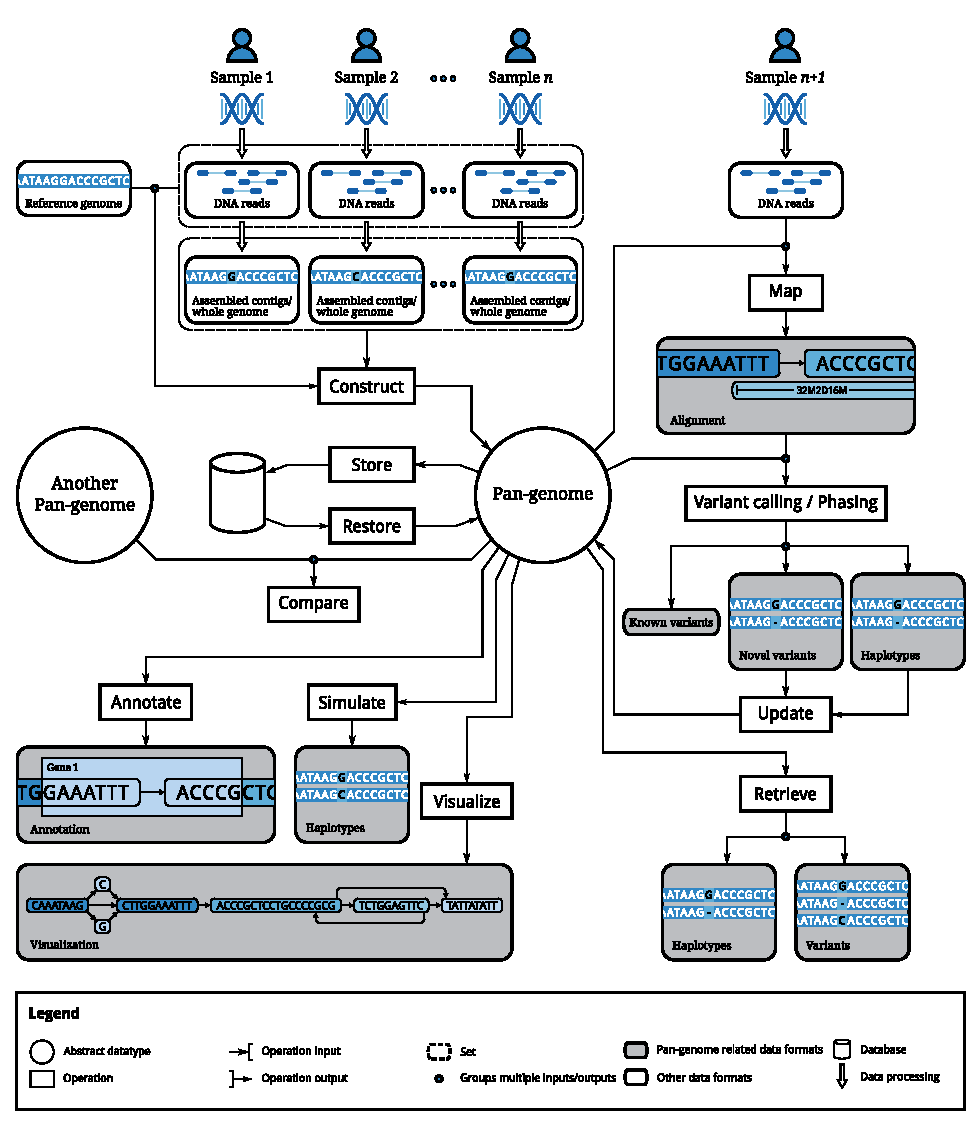
\includegraphics[width=1.0\textwidth]{Chapter1/Figs/cpang_fig2.pdf}
  \caption[Computational pangenomics]{
    An overview of techniques required to support pangenome-based resequencing.
    In {\tt vg}, we have implemented virtually all the presented components and algorithms.
    Reprinted from \cite{computational2016computational}.
    } 
\label{fig:pangenomic_processes}.
\end{figure}


% various approaches to encoding the pangenome

% think through, with references, the various ways we can resolve reference bias
% extended
\subsection{On pangenomic models}

\label{sec:on_pangenomic_models}

My own work builds on a particular model for encoding a pangenome.
Here, I will briefly describe alternative models and justify the use of the graphical one that I present, while the remainder of the chapter will provide background on more-closely related graphical approaches more closely related to my work.

Traditional techniques from microbial pangenomics have focused on cataloging the distribution of ORFs across bacterial species \cite{page2015roary}.
In this sense the pangenome is not so much a sequence-based object, but a matrix encoding the presence or absence of genes across the species of a given clade.

If we want to use pangenomic principles to resolve issues with resequencing, then we must take the concept of pangenome more literally, and build a representation that losslessly encodes genomes together with a focus on their sequence content.
In this perspective, the classical bacterial pangenome becomes a derivative product that we can produce using analyses based on a sequence-oriented pangenomic reference.
I will mostly focus on sequence-based pangenomic models.
The main classes are described visually in figure \ref{fig:pangenomic_models}.

\begin{figure}[htbp!]
  \centering
  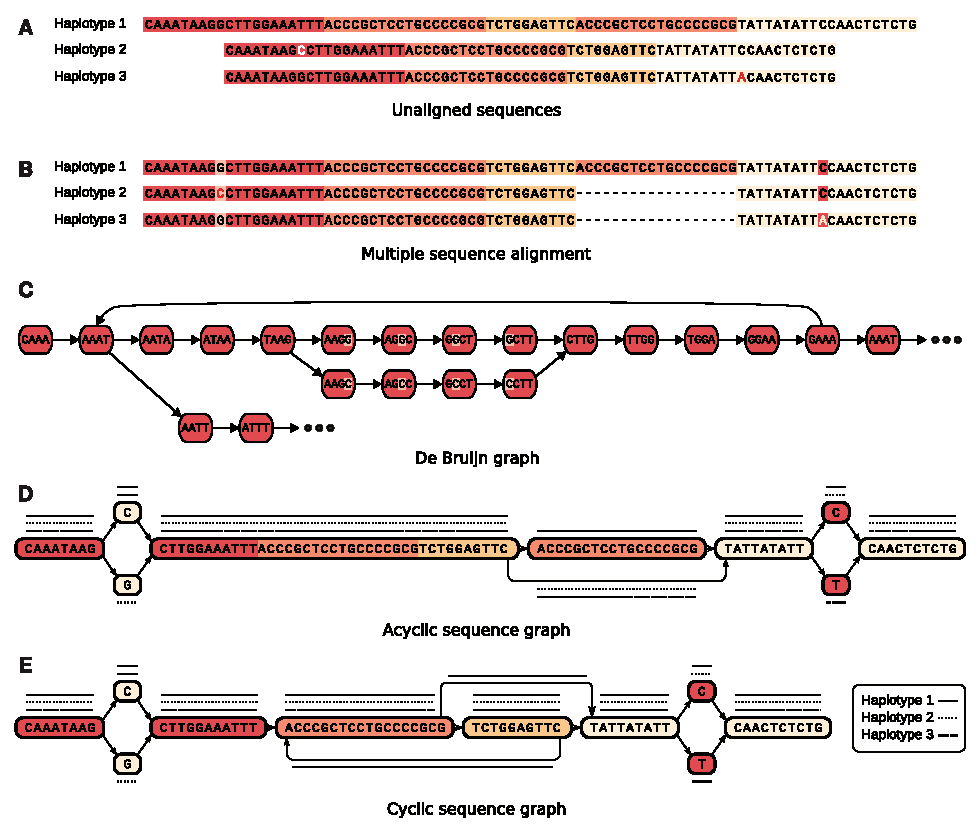
\includegraphics[width=1.0\textwidth]{Chapter1/Figs/cpang_fig3.pdf}
  \caption[Pangenomic models]{
    Various pangenomic models of a small collection of sequences.
    (A) shows an unfolded pangenome,
    (B) provides an MSA encoding the same sequences,
    (C) shows the DBG with $k=3$,
    (D) is an acyclic version of the pangenome, akin to the alignment in (B),
    and (E) represents a compressed alignment graph allowing cycles to represent copy number variants. 
    Reprinted from \cite{computational2016computational}.
    }
  \label{fig:pangenomic_models}.
\end{figure}

The simplest possible sequence-aware pangenome is just a set of whole genome sequences of many species or individuals, in which all sequence homologies and evolutionary relationships are implicit (figure \ref{fig:pangenomic_models}A).
The unfolded pangenome resolves reference bias, and can be extended with new data by simply including new genome sequences.
This model does not benefit from compression related to shared sequences in the pangenome, as adding a new genome always adds all the sequence in that genome to our system.
Without additional information about homologies, an unfolded pangenome cannot represent new sequences in terms of recombinants between known sequences.

An MSA (figure \ref{fig:pangenomic_models}B) provides a matrix describing the relationships between the sequences as well as the sequences themselves.
We must introduce a concept of a gap character to pad the matrix.
The MSA is a linear object, and cannot represent structural variation compactly.
An MSA has an equivalent representation as a sequence DAG, as in figure \ref{fig:pangenomic_models}D.

Assembly graphs, in particular DBGs (figure \ref{fig:pangenomic_models}C), provide a simple decomposition of collections of genomes.
However, a strict DBG without any labeling loses the mapping back to the original genomes.
Sequence graphs, as in figure \ref{fig:pangenomic_models}E, when annotated with the full set of input paths, provide a lossless representation of the input genomes.
If they are also bidirectional like DBGs (not shown in figure \ref{fig:pangenomic_models}E) then they can directly represent copy number variations and inversions.

\subsection{The variation graph}
\label{sec:the_variation_graph}

In this thesis I employ a reference system that encodes genomes and the base-level relationships between them.
This model can be understood as a kind of all-versus-all alignment between the sequences in the pangenome.
If the data model is to allow recombination between known sequences (a key contributor to genomic diversity) and tandem repeat copy number variation (which occurs readily in genomes), then it can be represented as a regular language encoded in a graphical model like a nondeterministic finite automaton (NFA).

We can adjust the regular language model slightly so that it has properties similar to those of DNA.
NFAs are represented graphically with states (in our case, pangenomic coordinates) as nodes connected by edges labeled by characters (e.g. DNA bases) in the alphabet of strings that the language recognizes.
In DNA the atomic element is the DNA base, which is represented as a character.
Graphical models with nodes (or edges) labeled by sequences and edges (or nodes) representing allowed transitions between them are a straightforward generalization of the linear string.
Compression can be achieved by allowing the labels on the nodes to have more than a single character on them.
Because DNA is double-stranded, any such a language implies a reverse complement language which recognizes the reverse complement of any sequence in the first.
Formalizing this by allowing edges to transition between different strands of the graph allows the model to directly represent sequence inversions.

If we combine these adjustments, we arrive at a kind of regular language model that resembles DNA and allows the representation of collections of related sequences by allowing us to represent homologous sequences and all kinds of natural polymorphism between them.
This structure is often referred to as a \emph{bidirectional DNA sequence graph}, indicating that the graph is sequence-centric, directed, stranded, and allows transitions between strands.
\emph{Sequence graph}, then implies a simpler concept in which the graph is meant to model sequences but only one strand is considered.
Assembly and multiple sequence alignment methods have employed sequence graphs of both types since the earliest computational analyses of biosequences, and it is sensible that we might employ them to represent collections of genomes.

The conceptual basis of the work I present here is the extension of the bidirectional DNA sequence graph with \emph{paths} that may be used to describe sequences as walks through the graph.
In this way, the panel of reference genomes or sequences used to construct the graph may be related to the graph itself, and the relationships between them made evident in the structure of the graph.
Existing knowledge expressed with respect to known sequences may thus be projected into the graphical pangenome model.
Similarly, entities within the graph may be \DIFdelbegin \DIFdel{``surjected'' }\DIFdelend \DIFaddbegin \DIFadd{projected }\DIFaddend out into the space of a given path \DIFaddbegin \DIFadd{(as described in section \ref{sec:surjection})}\DIFaddend .
These properties ensure that the pangenome fully encompasses existing reference technologies.
In addition, maintaining the sequences in the space of the graph makes the graph lossless, in that it fully represents the input sequences without additional information.
Perhaps most importantly, this feature resolves the exponential decay in mutual information which limits the applicability of Markovian models like the sequence graph to modeling natural sequences \cite{lin2017critical}.
I term this combination of a bidirectional sequence graph and paths a \emph{variation graph}, as it represents sequences and the variation between them.
In chapter 2 I will formalize the variation graph model and important auxiliary data structures that enable its modification and use in resequencing.

\section{Graphical techniques in sequence analysis}
\DIFaddbegin \label{sec:graphical_techinques}
\DIFaddend 

Many genome analysis algorithms employ sequence graphs.
I introduced the alignment algorithms described in \ref{sec:sequence_alignment} in terms of a matrix, but they may also be described as algorithms on graphs, although the nodes in these graphs correspond to matrix cells and thus alignment states rather than characters or sequences.
Similarly, hidden Markov models (HMMs) have a long history of use in bioinformatics \cite{durbin1998biological}, and these models bear similarities to the bidirectional sequence graph model.
Here, I will focus on those methods that are most closely related to variation graphs, and upon which my work draws most heavily.
These include techniques for generating and encoding multiple sequence alignments, genome assembly graphs, RNA splicing graphs, and the related gene model graphs used in RNA sequence analysis, and the sequence DAG implied by the VCF format.

\subsection{(Multiple) sequence alignment}
\label{sec:MSA}

Optimal multiple sequence alignment generalizes the problem of pairwise sequence alignment from a 2D matrix to an $N$-dimensional lattice, where the optimal mutual alignment of $N$ sequences of average length $L$ can be determined in $O(L^{N})$ time \cite{carrillo1988multiple}.
In the early days of sequencing, when only a handful of sequences might be considered in one analysis, such costs were almost acceptable, even if they limited the number of sequences in the MSA to only 3.
By pruning regions of the lattice in which no optimal alignments could occur, the authors of the tool ``MSA'' increased the number of sequences which could be optimally aligned into an MSA to 6 \cite{lipman1989tool}.
In contrast to the optimal alignment approach, progressive multiple sequence aligners such as CLUSTAL build a guide tree based on alignment of all sequences to all others in $O(NL^{2})$ time, and then generate the MSA progressively using the guide tree in $O(L^{2}\log N)$ time, resulting in polynomial time algorithms capable of generating MSAs for hundreds of sequences using contemporary computers \cite{higgins1988clustal}.
In this form of progressive alignment, the MSA is built recursively from the leaves to the root of the guide tree, with each step combining pair of MSAs representing different branches of the tree using the best pairwise alignment between the sequences they contain.
The progressive approach is fundamentally greedy, and susceptible to errors that propagate along the guide tree, although such errors can be mitigated by structuring the alignment using biological priors \cite{thompson1994clustal}.
Further improvements to the quality of the MSA can be gained by guiding the progressive alignment with a limited kind of global information about the relationships of all the sequences, as in T-COFFEE \cite{notredame2000t}, but this popular method exhibits a worst-case computational complexity of $O(N^{3}L^{2})$.

The progressive alignment in MSA algorithms like CLUSTAL may be represented graphically.
In the late 1980s Eugene Myers and Webb Miller developed algorithms to optimally align sequences to sequence graphs, and sequence graphs (in the form of regular expressions) to each other in $O(MN)$ time (where $M$ and $N$ are the sequence length of the graphs) \cite{myers1989approximate,wu1995subquadratic}.
Unfortunately, to my knowledge were never implemented in publicly available software for sequence analysis\footnote{Myers was unable to provide related source code on request.}.
A recent implementation of sequence to graph alignment \cite{rautiainen2018bit} transforms a sequence graph into an alignable graph which is acyclic and partially ordered, on which a bit-parallel alignment algorithm is applied to achieve high performance when aligning long noisy reads to arbitrary sequence graphs.
This work is related to that of Wu, Manber and Myers \cite{wu1995subquadratic}, wherein the authors provide an algorithm for the alignment of pairs of regular expressions using a transformation of the regexes to NFAs and bit-parallel resolution of the final alignment.
Later in chapter 2 I will present and evaluate a similar approach to align reads to arbitrary bidirectional sequence graphs through transformation of the graph into an ordered graph against which accelerated sequence to graph alignment may be run.

Christopher Lee later provided the first implementation of an MSA algorithm based on sequence to graph alignment \cite{lee2002POA}.
Apparently unaware of the work of Myers and Miller, he instead built on the concept of ``consistent equivalence relations'' that DIALIGN used to represent the MSA \cite{morgenstern1996multiple}.
Where DIALIGN's authors appear to consider the MSA in the space of the $N$-dimensional lattice, Lee encoded the equivalence relations in a partial order graph, which is often referred to as a directed acyclic graph (DAG).
In this DAG, characters label nodes and edges label observed linkages between them in sequences embedded in the MSA.
Lee demonstrated that a straightforward generalization of the recurrence relations used in Smith-Waterman-Gotoh would allow the alignment of sequences of length $N$ to the DAG of sequence length $M$ in approximately $O(MN)$ time.
To determine the score at a given position, partial order alignment (POA) considers matches and deletions relative to all the characters that immediately preceded the current one in the partial order.
Later, POA was extended to allow the direct alignment of pairs of MSAs using partial order to partial order alignment (PO-POA) \cite{grasso2004combining}.
Like CLUSTAL-W and other progressive methods, POA would build its MSA using pairwise alignments across a guide tree.
But, rather than aligning the last pair of sequences, PO-POA alignment would be used to align the MSAs from each branch together.
This resolved problems with order dependence, yielding MSAs with nearly the same accuracy\footnote{Here goodness is quantified using a sum of pairs score (SPS) metric representing the goodness of the alignment.} as T-COFFEE across a range of problems.
As PO-POA proceeds over a neighbor joining guide tree, it requires $N \log{N}$ alignment steps.
Given low sequence divergence, the cost of each step will approximate $L^2$.
The algorithm thus has a lower bound of approximately $O(L^{2}N\log{N})$, which the authors confirmed with experiments demonstrating subquadratic scaling in the number of input sequences.

Despite its use of an algorithm that scales cubically with the number of input sequences, T-COFFEE's higher accuracy has resulted in it receiving ten times the citations of POA.
The low rate of use meant that the POA concept was ``rediscovered'' by participants in the 1000GP who
needed a computationally inexpensive method to align sequences to VCF-based pangenomes\footnote{Sequence to graph DAG alignment was one of Deniz Kural's main PhD projects. I worked with him in Gabor Marth's laboratory, and we applied his implementation of POA to generate accurate genotype likelihoods for indels and complex variation in the final phase of the 1000GP. We learned of the prior work later, when a reviewer pointed out that the algorithm was roughly equivalent to POA.}.

Lee's POA model provides a simple pattern for thinking about pangenomes.
However, POA MSAs are linear objects which cannot capture many natural kinds of genetic variation such as repeats or rearrangements without duplication of the rearranged sequences.
Several methods have extended the MSA concept to unordered graphs, including the Threaded Blockset Aligner (TBA) \cite{blanchette2004aligning}, which models the MSA graph as a set of partially ordered MSAs linked by unordered larger scale connections, and the A-Bruijn Aligner (ABA), which models the MSA using a de Bruijn graph and represents a solution to problems in MSA using techniques that later become important to short read assembly \cite{raphael2004novel}.
Variation graphs generalize these models without the limitations of order (as in POA and TBA) or $k$-mer based graph structures (as in ABA).

\subsection{Assembly graphs}

The problem of assembling large genomes is not dissimilar from that of multiple sequence alignment.
MSA algorithms tend to be applied to the alignment of a single coherent genomic locus.
Their input sequences might be expected to have approximately the same length, and maintain synteny between them.
In contrast, whole genome shotgun assembly methods cannot rely on such assumptions, as reads of a large genome rarely overlap, and both strands of DNA will be sampled, yielding ambiguity about relative orientation.
Thus, the graphical models used in assembly must maintain bidirectional structure.
OLC assembly methods in some sense began their evolution with the set of compromises that MSA algorithms ended theirs, with thrifty heuristic methods being used to establish the overlaps between all pairs of sequence reads from a given genome, and the resulting overlap set subsequently represented graphically.
Earlier in section \ref{sec:genome_assembly} I gave a historical outline of the development of these methods in response to changes in available sequencing technology.
Here, I provide deeper technical detail to describe these methods and illustrate their relationship to the variation graph model.

\subsubsection{Overlap graphs}
\label{sec:overlap_graphs}

One interesting feature of overlap-based assembly graphs is that their efficient construction tends to yield a representation in which sequences attached to nodes partially overlap with the nodes in their neighborhood in the graph\footnote{In many formulations, sequences in the overlap graph are attached to edges rather than nodes. This model is equivalent to one in which sequences are attached to nodes, which I will use here for consistency. The same convention is used in {\tt vg}'s data model and in the GFA interchange format that it reads and writes.}.
This follows from the fact that the graph induction algorithms use a kind of pairwise alignment, retaining relationships between sequences in a pairwise rather than compacted N-wise form.
In the case of DBGs and the FM-index based string graph assemblers, an iterative overlap-wise sequence comparison where unitigs (unbranching sequences in the graph) are inferred from the compressed sequence graph yields overlap graph.
Given a node-labeled sequence graph, it is common to think of the edges as representing the overlaps between the nodes they connect.
This represents an incomplete compression of the relational information in the graph, but this is typically not important to the use of these methods.
They are judged by the quality of the set of contiguous sequences (contigs) they output rather than their raw assembly graph.
These methods will traverse linear portions of the graph to generate contigs, after pruning or ignoring edges, which the uncompressed overlap representation does not inhibit.

Due to its duplicated representation of sequences within overlaps, the overlap graph model is more complex to use as a reference system (in which positions should be unique) than a ``bluntified'' representation in which the overlaps are non-ambiguously reduced into the nodes in the graph and its linkage topology.
In their most general form, overlaps are themselves alignments, and have a natural encoding in graph form (section \ref{sec:MSA}).
However, assembly data models often encode alignments using several dissimilar data structures, a fact which is reflected in the complexity and redundancy of the GFA version 2 specification\footnote{\url{https://github.com/GFA-spec/GFA-spec/blob/master/GFA2.md}}.
In general this overlap representation makes it difficult to work directly with such graphs using the algorithms we will introduce, and they must be reduced into a ``blunt-ended'' bidirectional graph.

% mention miniasm and friends, bit of grounding in the present

It is also possible to directly induce a bidirectional string graph from a set of pairwise alignments, sidestepping the overlap issue.
In section \ref{sec:from_pairwise_alignments} I will present my design and implementation of an external memory algorithm that transforms sets of pairwise alignments into a variation graph using a transitive closure of the equivalencies implied by the alignments.

\subsubsection{De Bruijn graphs}
\label{sec:de_bruijn_graphs}

De Bruijn graphs \cite{de1946combinatorial} are graphs in which a set of $k$-mers are taken as the nodes of the graph, and edges are added for each pair of $k$-mers $k_1 \rightarrow k_2$ in which the last $k-1$ bases of $k_1$ are the same as the first $k-1$ bases of $k_2$.
As discussed previously in section \ref{sec:genome_assembly}, this model simplifies the overlap graph structure, allowing efficient calculation and representation of the graph.
For instance, $k$-mer lengths may be chosen so that they fit inside a machine word, allowing bitwise operations and integer math rather than string comparison to be used to infer the graph structure directly implied by the $k$-mers themselves.

In second generation sequencing, where per-base error rates are low and read lengths are short, little information is lost by breaking the read set into $k$-mers of 1/3 or 1/5th the length of the original reads, and so the de Bruijn graph model has been readily applied to cheap short read sequence data since its introduction to genomics in the mid 1990s and early 2000s \cite{idury1995new,pevzner2001eulerian}.
Velvet \cite{zerbino2008velvet}, which used a straightforward but memory-costly hash table strategy to encode the DBG.
Zamin Iqbal then extended the DBG model to support various kinds of pangenomic analysis by labeling each $k$-mer with ``colors'' representing read counts from different samples \cite{iqbal2012novo}.
The colored DBG (cDBG) model has seen application in RNA-seq transcript quantification, where the model is used as a reference basis for the relation of known transcripts to pseudoalignments of reads to the cDBG \cite{bray2016near}.
Later versions of the Cortex assembler have extended this to fully encode long reads or contigs relative to the DBG \cite{turner2018integrating}.
Similarly, improvements in performance have been yielded by linking read pairs in the DBG model \cite{bankevich2012spades}.

The simplicity of the DBG has made it possible to develop very memory-efficient data models to support its use in assembly.
The DBG can be effectively encoded in the FM-index of a read set \cite{bowe2012succinct}, and this \emph{succinct} DBG model underpins the most-scalable assembly methods currently available \cite{li2015megahit}.
Other techniques, such as bloom filter encodings and minimizer partitioning schemes are also used to provide time and space efficiency to DBG methods \cite{chikhi2013space, chikhi2016compacting}.

In the compacted DBG generalization non-furcating regions of the graph are merged into a single node with label length $>k$.
The compacted DBG is now often a typical output for DBG assemblers \cite{chikhi2016compacting,minkin2016twopaco}.
The compressed nodes and their overlaps with their neighbors comprise a set of unitigs that, together with their neighbor relations, are often taken as the most-raw kind of assembly output.
DBG assemblers like SPAdes and Minia3 infer longer contigs by filtering and further contracting the unitig graph \cite{bankevich2012spades}.

As with any overlap graph, DBGs must be made into blunt-ended sequence graphs before they can be utilized by variation graph based algorithms.
The basic method for doing so is simpler than for generic overlap graphs, as overlaps in DBGs are exact string matches.
In my work I have found this an important feature, as in addition to being generated by efficient methods, it ensures that DBGs are universally convertible into variation graphs.

\subsubsection{String graphs}
\label{sec:string_graphs}

The string graph is a formalism that describes the full information represented by a shotgun sequencing experiment and an all-against-all alignment between its reads \cite{myers1995toward,myers2005fragment}.
Myers argued that the then-current paradigm of assembly, which attempted to generate the shortest common superstring (SCS) incorporating all the $N$ input sequence reads, failed to reconstruct the genome correctly in the context of repeats in the genome that are longer than the average read length $L$.
He then posited the ``chunk graph'' (later, string graph) as a graphical model of the overlap set, showing that the correct consensus sequence would by definition exist as a walk through the graph, and that constraining the collapse using coverage information would improve reconstruction of the genome read in the shotgun sequencing experiment.
In this graph nodes (or edges) represent sequence reads and directed edges (or nodes) represented observed $\epsilon$-approximate overlaps between them.
Repeat units in the genome that are longer than $L$ will collapse in this graph, provided errors in the reads can be corrected so such repeats become fully identical.

This idea was introduced at the same time as de Bruijn graphs, with Myers' work on string graphs and the first description of a genome assembly algorithm using de Bruijn graphs both presented at the same workshop in 1995 \cite{myers1995toward,idury1995new}.
Myers' 2005 formalization of the string graph \cite{myers2005fragment} responds particularly to de Bruijn models, and he points out that generating $k$-mers from the reads as the basis for the graph means that the resulting graph is not ``read coherent'', or in other words does not accurately represent the information in the read set.
Subsequent work has shown that the boundaries between the two models are not so well-defined.
As a specialization of the overlap string graph, the de Bruijn model may be applied to certain complex subsets of a string graph, creating a kind of hybrid assembler where the $k$-mer model is used to resolve the most-difficult components, while the generic overlap model is used elsewhere \cite{huang2016integration}.
Similarly, the high cost of error and graphical complexity suffered by the string graph encourage the use of $k$-mer based read correction methods, which could be seen as filtering the reads using a DBG model.

String graphs are often described as ``lossless'' representations of the input read set and the alignments between them \cite{li2012exploring}.
Neither in practice, in Myers' formalizations, nor its implementations like the Celera assembler (CABOG) \cite{miller2008aggressive} is this strictly true.
In the model, overlaps are assumed to be $\epsilon-$correctable at approximately the raw sequencing error rate.
In practice, this filtering can result in a loss of input sequence from the string graph.
String graphs can consume very large amounts of memory when fully constructed without filtering from a read set \cite{li2016minimap,koren2017canu}.
Input filtering, mostly to reduce repeat content, is used to mitigate this issue.
If not aggressively corrected, repeats tend to generate ultra-dense graph regions that are known as ``hairballs'' which can increase the complexity of assembly by orders of magnitude.

To deal with repetitive sequences in the genome, one solution is to mask out repetitive $k$-mer, minimizer, or alignment seeds used in generating the overlap set, as in CABOG, FALCON, and miniasm \cite{miller2008aggressive,chin2016phased,li2016minimap}.
Recently, the authors of Canu showed that alternative probabilistic seed filtering based on the \emph{tf-idf} (term frequency, inverse document frequency) metric can retain information about repeats and support their separation rather than excision from the assembly string graph \cite{koren2017canu}.

String graph methods related to the Celera assembler, such as FALCON and Canu, implement error correction steps before overlap inference, as this reduces memory requirements during assembly.
Similarly, methods that generate assemblies via a string graph induction step from Illumina sequencing data (SGA, fermi, and fermikit) also apply an error correction processes before the generation of the string graph \cite{simpson2012efficient,simpson2014exploring,li2015fermikit}, which helps to reduce the graph complexity and improve contiguity of the resulting assembly.

Allelic diversity in either a string graph or de Bruijn graph will, if sufficiently separated from repeats and other allelic variants, result in a bubble, or graph component connected to the rest of the graph via single sources and sinks.
Like de Bruijn graphs, string graphs have been used to support variant calling, for instance finding heterozygotes represented as bubbles in the assembly graph \cite{li2012exploring}.
All methods that I am aware of will establish variants relative to a reference sequence threaded through the graph.
Also, thus far no method has specifically merged the two concepts of variant calling and graph based assembly finishing together, although assembly projects may use a variant caller to establish variants in their contigs \cite{jain2018nanopore,schmid2018pushing}.

With minimap and miniasm Heng Li took the approach of efficient all versus all alignment and overlap graph generation without prior read correction \cite{li2016minimap}.
With no multiple alignment step, this generates an assembly in which the error rate in the contigs approaches that of the input reads.
Tools like racon \cite{vaser2017fast} have been developed to subsequently generate a consensus, but these work on the level of individual contigs rather than an assembly graph.
Li \cite{li2016minimap} also proposed to mix and match different assembly components (for instance using DALIGNER \cite{myers2014efficient} rather than minimap for the overlap step, or swapping quiver for nanopolish for consensus generation) by establishing a set of standard data types including the pairwise alignment format (PAF) and the graphical fragment assembly (GFA).
These encode the results of the overlap step and a graphical model for the assembly at any state of its progression.
GFA is used in a wide number of methods, but as of August 2018 it appears that very few tools both read and write GFA\footnote{\url{https://github.com/GFA-spec/GFA-spec\#gfa-1}}, and much of the assembly improvement steps are implemented on contigs (encoded in FASTQ or FASTA format) rather than the string graph itself.

% it's an overlap graph yep

\subsubsection{RNA sequencing graphs}
\label{sec:rna_seq}

While many approaches to transcript analysis consider each particular gene transcript separately, a more compact representation would be as a \emph{splicing graph} in which all alternative splicing junctions are represented by edges connecting bases of the underlying reference sequence \cite{heber2002splicing,lee2002POA}.
Transcript assembly has attracted many of the same approaches as those used in genome inference, but their application must be adjusted to account for variation in read coverage of several orders of magnitude caused by large differences in expression of different genes \cite{martin2011next}, and in some cases they may not be suitable as the ideal of a transcript assembly is not a linear sequence assembly, but a splicing graph that models the combinatorial relationships in the transcriptome \cite{grabherr2011full}.
Standard assemblers, parameterized or modified to better support RNA transcript assembly have been applied to the problem since their development for genome assembly \cite{birol2009novo,robertson2010novo,schulz2012oases}.
But methods which are specifically design to meet the needs of the problem have arguably been more popular \cite{grabherr2011full,chang2015bridger}.

Direct use of the splicing graph concept is limited, with the most-popular workflow involving ``splice-aware'' alignment to a reference transcript model followed by quantification of expression versus the alignment and transcript model \cite{trapnell2012differential}.
More recently, probabilistic approaches have come into favor, and to support these assembly models have been applied to transcript quantification via pseudoalignment to a colored DBG annotated with reference transcripts \cite{bray2016near}.
In contrast, Daewan Kim's HISAT2 aligns RNA-seq reads to a whole genome splicing graph \cite{kim2015hisat,kim2017hisat2}, including SNP and indel variation directly in the whole genome index.

\subsubsection{Genome alignment graphs}
\label{sec:genome_alignment_graphs}
The graphs used in genome alignment algorithms are the nearest in content and structure to variation graphs, and it can be shown than a number them of nearly identical representational capacities \cite{kehr2014genome}.
The \emph{alignment graph}, first introduced in the context of multiple sequence alignment \cite{kececioglu1993maximum,rausch2008segment}, represents a collection of alignments in graphical form, supporting the induction of a sequence graph (or MSA when such a graph is partially ordered).
Vertices in the alignment graph $G_a = (V, E)$ represent characters in the input sequences $S$, and edges represent cases where characters in the input sequences have been aligned, with an additional relation $\prec$ on $V$ such that $v \prec w$ holds if and only if $v$ precedes $w$ in $S$.
As it contains both the sequences and their alignments, this graph may then be contracted to produce a compressed graph that represents both.
We can then contract $G_a$ into the base graph $G_s$, adding a node for each connected component in $G_a$ and labeling it with the corresponding character, while adding an edge for each pair of nodes $X$ and $Y$ which represent a pair of input characters in $G_a$ that satisfy $\prec$.
Each column of an MSA matrix or each base in a variation graph would correspond to a particular connected component in $G_a$.
It is worth noting that the equivalence is not exact unless we generalize the alignment graph to represent alignments in both the forward or reverse complement orientations, which has been explored in the A-Bruijn model \cite{raphael2004novel}.

The Enredo graph model $G_e = (V, E)$, used by Benedict Paten's Enredo/Pecan multiple genome aligner \cite{paten2008enredo}, generalizes the alignment graph model to be bidirectional by representing each genome segment in the graph with two nodes, a head and tail.
The graph maintains two kinds of edges, $E_s$ which represent genome segments and are equivalent to nodes in $G_s$, and $E_a$ which represent breakpoints of adjacencies between segments.
To obtain a graph like $G_s$ from the Enredo graph, the MSA resolver Pecan is applied to sets of homologous $E_s$ connecting the same head and tail nodes.

Paten further refined multiple genome alignment by the development of the Cactus graph $G_c = (V,E)$ \cite{paten2011cactus}.
To construct the Cactus graph, we build a precursor graph $G_c'$ by adding a node for each adjacency-connected component in the Enredo graph $G_e$ and adding edges between nodes for each segment $E_s$ whose head and tail lie in both adjacency components.
To obtain the Cactus graph, we collapse three-edge connected components in $G_c'$ into single nodes, yielding an Eulerian graph with a tree like structure.
The nodes in the Cactus graph can be shown to correspond to a tree of \emph{ultrabubbles} (graph components connected to the rest of the graph by one or two head and tail nodes) in the sequence graph from which it was constructed \cite{paten2018superbubbles}.
This forms the basis for the development of genotype models on top of arbitrary graphs.

Without additional labeling, these graph models are insufficient to fully reproduce their input, and although it may be implemented in corresponding software, existing models to do not clarify how this labeling is accomplished \cite{kehr2014genome}.
Variation graphs respond to this issue by making the path embedding of the sequences in the graph explicit in the model.

\subsection{Pangenomic alignment}

As the review presented in this chapter shows, the idea of using pangenomic models as a reference basis is not new, and interest in the topic extends back to the earliest explorations of the multiple sequence alignment problem.
But it was only in the last decade, as surveys of populations of genomes routinely produced sets of phased variant calls \cite{liti2009population,weigel20091001,cao2011whole,1000Gphase1,1000g2015} that the idea of scaling up alignment to enable the alignment of short reads to populations of genomes gained traction.
Numerous methods use some form of pangenome aware alignment.
These have helped me to understand the problem and guided my work to a significant degree.
Each has important limitations relative to more generic problems.
For instance, some operate on sequence DAGs, and cannot easily be generalized to work on arbitrary bidirectional sequence graphs.
Others implement a limited form of alignment that prevents their use for every kind of sequencing technology.
Virtually all use the pangenome only as an additional source of information during alignment, and do not use the pangenome as the reference system itself.

\subsubsection{Alignment to unfolded pangenomic references}

As discussed in section \ref{sec:on_pangenomic_models}, the simplest pangenomic model stores each genome sequence individually, without recording the implied homologies or relationships between the sequences.
Such a model grows linearly with the number of genomes included, and in this way it does not benefit from compression provided by sequence relationships and shared evolutionary histories.
Annotations can be provided for each genome and interlinked at a higher level of semantic relationships, as is done in major genome annotation catalogs like Ensembl genomes \cite{kersey2015ensembl}.
This expedient approach provides almost all the benefits of the kind of pangenomic models I present in this thesis, excepting that it cannot represent base-level sequence relationships within the semantic model without significant effort.
Whenever a researcher uses BLAST or BLAT to search a large database of sequence they are interrogating this ``unfolded'' pangenome.
This pattern could be thought of as the default in bioinformatics, and it is the starting place for many DNA-based analyses.

In terms of methods specifically designed to align large sequence read sets against an unfolded pangenome, few are currently under development.
Of note, the CHIC aligner provides an initial implementation of such an idea \cite{valenzuela2017chic}
This method is based on an indexing strategy which uses Lempel-Ziv (LZ77) \cite{ziv1977universal} parsing of the pangenome to generate a ``kernel'' sequence encoding the pangenome that may be indexed and used by a standard short read aligner (the authors use BOWTIE2).
By using this kernel, the seeding step is aware of alternative sequences embedded in the pangenome, but the local alignment step is ultimately run against a linear reference.
As this approach aligns directly to the unfolded pangenome it is not able to correctly estimate mapping quality, as the reference does not encode any model about the relationships between the genomes that comprise the pangenome and consequently we cannot determine when multiple alignments match to homologs in different genomes or paralagous copies dispersed across one or many genomes.
The linear growth in data scale can add algorithmic complexity when sequencing many genomes, and so it is understandable that experiments using the CHIC aligner only used up to 100 genomes at a time.
By relying on the linear reference to report alignments, CHIC gains the ability to hook into standard resequencing workflows, but it loses the ability to describe variation in sequence that is not contained in the reference.

%It is not clear yet if this model will be usable with practical inputs, and it is clear that it will not be able to encode other commonly-used graphical models for representing populations of genomes.
%Techniques from compressed data structures have been used to resequence short reads against the unfolded pangenome, as implemented in the CHIC aligner \cite{valenzuela2017chic}, but numerous problems have prevented the exploration of this modality.
%We can use this work to understand some limitations of this approach.


\subsubsection{Alignment to tiled pangenomic references}

A near-approximation of the unfolded model is one in which genomes are broken into small pieces in the construction of the model.
These blocks or tiles can then be formed into sequence DAG by the addition of edges showing linkages between successive blocks \cite{guthrie2015tiling}.
These models present as a specialized kind of sequence DAGs\footnote{Known implementations appear to be unable to directly represent inversions and copy number variants in their structures, instead encoding them as if they were indels.}, and can represent the whole set of sequences in a pangenome in a semi-compressed way using the same principles as in POA, DBG, or string graph models.
Each tile represents a known haplotype in a given window of the pangenome.
As new genomes are added to the structure, new tiles only need to be added where we observe a new sequence in a given window.

A tiled pangenome graph was employed by the pangenomic aligner, GenomeMapper \cite{schneeberger2009simultaneous}, which was produced in support of the \emph{Arabidopsis thaliana} 1001 Genomes Project (AT1001GP).
As arabidopsis frequently selfs, individuals may have extremely low levels of genomic diversity, which in turn simplifies the process of genome inference \cite{cao2011whole}.
At the same time, several percent of the reference genome is missing or highly divergent in various accessions (strains) \cite{clark2007common,zeller2008detecting}.
These conditions break standard short-read aligners developed for mapping Illumina sequencing data against low-diversity reference genomes.
GenomeMapper models the pangenome using 256 basepair tiles.
A $k$-mer index is used to seed local alignment of very short (<50bp) reads against the pangenome.
The authors report an extension of the Needleman-Wunsch alignment algorithm that allows alignment against the graph wherein the graph traversal is converted into a tree of alignments by duplicating the alignment process at each furcation.
This alignment algorithm is exponential in the average number of forks per sequence base, which may contribute to the observation that it runs hundreds of times slower than standard alignment methods on 100bp reads \cite{liu2016debga}.
GenomeMapper does not have a graph-specific alignment format, and instead reports alignments against the genome to which each is most similar, which the authors call ``reference free''.
So that the alignments may be used downstream in standard approaches, they may be projected against another chosen reference genome.

\subsubsection{Alignment to graphical assembly models}

In order to report their results relative to the reference, assembly methods require the ability to align the reference genome into the sequence graph they have generated \emph{de novo} \cite{iqbal2012novo,simpson2012efficient}, although this can be achieved through the alignment of the assembly graph's unitigs to the reference genome \cite{li2015fermikit}, which results in greater sensitivity to small variation but may also increase bias towards the reference genome.
Aligning external sequence to an assembly graph is equivalent to extending the assembly to include the sequence and recording the path through the assembly graph that represents it.

The deBruijn Graph Aligner (deBGA) inverts this approach by enabling the alignment of short reads to a reference DBG (RdBG) \cite{liu2016debga}.
An RdBG is a compacted DBG in which one or more reference genomes have been embedded, and the authors of deBGA enable alignment against it through a $k$-mer index that is used to drive a kind of MEM-based seed and extend alignment.
The alignment process itself attempts to link patterns of $k$-mer hits in unitigs in the graph into larger alignments, finally producing a local alignment by applying Smith-Waterman-Gotoh to the read and the particular reference genome region to which it aligns.
While deBGA uses a DBG to structure alignment, it can output a BAM file against the linear reference genome for use in variant calling or other analyses.
The authors claim that deBGA is fast and, thanks to its use of a DBG-based index, robust to alignment problems introduced by repeats.
However, it is not clear how the method develops mapping qualities, and due to its inability to represent evolutionary homology or equivalence between regions of genomes, this would appear to be is a significant limitation of the reference data structure they have chosen.

deBGA is the first published method specifically designed to align short reads against arbitrarily-structured graph genomes.
While deBGA was designed to work on collections of linear references, the authors note that it would also be possible to apply the indexing strategy to any sequence graph, as $k$-mer enumeration may be used to convert any sequence graph into a DBG\footnote{Jouni Sir\'{e}n and I had implemented an aligner based on a DBG transform of an arbitrary sequence graph at the time of deBGA's publication. The authors of deBGA were apparently as unaware of our work as we were of theirs.}
The authors do not evaluate its operation on generic DBGs, and instead compare it to linear reference based aligners on the same collections of genomes.

\subsubsection{Genotyping using a sequence DAG}
\label{sec:seq_dag_vcf}
Variant calls in the VCF format, when combined with the reference genome to which they refer, form a sequence DAG that encodes all the genomes from which the calls were derived as well as novel recombinations between them.
As this feature of variant calls was appreciated, it led to the development of several methods which first map reads globally to a linear reference and then realign them locally to a variation-aware reference.
This can be shown to reduce reference bias, but it can only do so in a localized sense as this form of graph resequencing cannot change the global placement of reads.

By the final phase of the 1000GP \cite{1000g2015} it was apparent that indels and complex variation were more difficult to genotype than SNPs.
Their significance was appreciated by 1000GP subprojects that examined the putative functional effects of such variants \cite{challis2015distribution}, which motivated efforts to develop a high-quality variant set including them for the final release.
The best-performing methods for generating the SNP genotype likelihoods (GLs) were only able to model biallelic SNPs \cite{snptools}, and additional methods would be applied to derive GLs for non-SNP, non-biallelic variant types.

While participating in the project, Deniz Kural and I extended (as glia\footnote{\url{https://github.com/ekg/glia}}) a POA algorithm he had developed to realign poorly-mapped reads (such as those with softclips, many mismatches, gaps, or unaligned fragments anchored by their pair mates) to a sequence DAG created from the reference and candidate alleles in the region.
By projecting the alignment back into the reference space, we were able to generate a BAM output from glia.
I implemented improvements to freebayes that allowed it to genotype alleles represented by observations in these alignments, as well as contamination estimates that were essential to high-quality GLs in low-coverage data.
This pipeline outperformed alternatives, and was ultimately used to generate GLs for all non-SNP variation in the project.

The indels were integrated into the phased scaffolds provided by the SNPs through two cycles of genotyping.
In the first, GLs generated by the method were given to MVNcall \cite{menelaou2012genotype}, a multalleleic, site-independent phasing algorithm that can phase genotypes at a given site onto a fixed background haplotype scaffold.
The posterior genotype and phasing quality estimates produced by MVNcall, along with a number of other metrics related to indel sequencing error such as sequence entropy and homopolymer context, were then used to establish a support vector machine (SVM) classification model which was trained using data from high-quality genomes and applied to the full set of alleles to remove likely errors.
The final set of alleles were fed back through the glia, freebayes, and MVNcall process to ultimately produce the set of indels in the 1000GP phase 3 release.

Hannes Eggertson's GraphTyper \cite{eggertsson2017graphtyper} implements a similar workflow to the genotype likelihood generation method applied to the 1000GP indels.
In the GraphTyper pipeline, Illumina reads are aligned against the reference genome using a standard short read aligner.
Those alignments with soft clips and apparent differences from the reference are matched to a sequence DAG built from the reference and VCF in a window around the read's candidate mapping location.
GraphTyper matches short $k$-mers between the read and the sequence DAG using a $k$-mer index of the reference structure and 1bp-overlapping $k$-mers from the read.
This does not produce an alignment \emph{per se}, but rather a list of variant traversals supported by each read.
This transformation provides sufficient information to genotype the variants in the graph.
The pipeline may update its reference system so that it includes both known variation from other studies and new variation discovered during analysis.
GraphTyper uses the graph reference system internally to improve algorithm performance, but results are projected into the linear reference and the graph has no other representation than VCF.
This prevents the representation of ``nested'' variation or non-SNP or indel SVs.
GraphTyper's efficient and accurate performance on exceptionally large resequencing problems supports the authors' design decisions and firmly asserts the utility of the graph realignment approach.

Sibbesen and colleagues generalize the genotyping problem to arbitrary variation graphs with BayesTyper \cite{sibbesen2018accurate}.
They adopt a kind of pseudoalignment model in which exact $k$-mer matches between a read set and the reference are used to establish support for paths across bubbles in the variation graph.
These can then be used to build probabilistic models of genotypes for any kind of variation represented in the graph, both small (SNPs and indels), including nested variation.

\subsubsection{Population reference graphs}

Pangenomic references need not be used as a coordinate system in the same manner as the linear reference genome.
Instead, they can be used as a prior to infer most-likely underlying haplotypes of a given individual.
Further refinement can be achieved by aligning the read set back to the inferred haplotypes.
This approach makes sense if alignment against the pangenome is extremely costly, but efficient haplotype inference patterns can be applied to the genome.

Population reference graphs (PRGs) \cite{dilthey2015improved} are POA-like graphs in which sequences aligned by MSA are collapsed in the case of identity above a given $k$-mer size, which embeds some information about local phasing into the graph.
First assembled from long sequences, the PRG is then augmented with local variation information, with SNPs and indels added to all paths at appropriate positions.
Dilthey and colleagues develop a genome inference model based on the comparison of the PRG to a DBG built from reads from a given individual.
By comparison between these two structures, weighted by $k$-mer frequency in the genome and PRG, they provide sufficient annotations to the PRG to run an HMM on the graph to infer the most-likely underlying pair of haplotypes.
Short read alignment can be used to map the full reads back to these haplotypes in an \emph{ad hoc} manner in order to find new small variation against them and fully resolve their sequences.
The authors demonstrate that this method can be applied to the human MHC, where high sequence diversity frustrates methods optimized for typical regions of the human genome.

\subsubsection{Succinct pangenomic sequence indexes}
\DIFdelbegin %DIFDELCMD < 

%DIFDELCMD < %%%
\DIFdelend \DIFaddbegin \label{sec:pangenomic_sequence_indexes}
\DIFaddend %Given a sequence DAG 
% write the DAG into the index provided a number of structural limitations
% problems with nesting (yes could be corrected) and cost of large alphabet WT based FM-index

Generalizations of the FM-index to support indexing of sequence DAGs, or equivalently regular languages, yielded a number of short read to sequence graph aligners.
Such methods enable pattern matching against pangenome graphs in much the same way as done by FM-index based short read aligners.

The Generalized Compressed Suffix Array (GCSA) \cite{siren2011indexing,siren2014indexing} enables pattern matching against arbitrary finite regular languages.
It indexes a reverse-deterministic automaton\footnote{Reverse determinization ensures that each prefix of this automaton can only have a single starting position.} that encodes the sequence DAG implied by a VCF and reference genome.
To enable path queries, it builds the BWT based on the sorted prefixes of the language encoded in the automaton, adding support structures that allow pattern search as in an FM-index.
Additional support bitvectors akin to those used to encode and index labeled trees \cite{ferragina2005structuring} allow the traversal of the sequence DAG during query matching.
Sir\'{e}n constructs the index using the prefix-doubling method used to construct sorted suffixes, wherein prefixes and their starts and ends may be extended from length $L$ to $2L$ through a sort and join operation.
Because it indexes a memoryless automaton and the construction requires the enumeration of all the prefixes of the automaton, GCSA suffers from exponential costs in index generation in the order of the number of possible recombinations represented in the sequence DAG.
Careful curation of the pangenome allows the construction of the GCSA for the entire human genome in the memory of an available computer (1TB), provided the construction is broken into chromosomes and local complexity in the input sequence DAG is reduced.
Experiments with the GCSA used backtracking search as in BWA \cite{li2009fast} to directly align reads with differences from the indexed graph, but the method was not developed into a full-featured short read alignment method.

Alternative schemes make no fundamental change to the CSA/FM-index model, but rather embed information about particular kinds of pangenome graphs into the sequence that is indexed.
BWBBLE \cite{huang2013short} encodes SNPs by extending the reference alphabet to include ambiguity codes which match more than one DNA base.
To encode indels, it extends the reference by adding a sequence for each indel which includes the non-reference allele and the surrounding $2l$ bases of the reference.
The resulting index can support queries of up to length $l$.
A mapping between the positions in the extended reference and the original reference sequence space is used to project alignments from the extended reference to the base reference.
This approach is simple and allows for a linear-time indexing of the pangenome, but the added complexity of the extended reference and larger alphabet required to represent SNPs yield a query time that is 100-fold slower than the backtracking BWA method \cite{huang2013short}.

In gramtools \cite{maciuca2016natural}, a particular kind of sequence DAG is indexed in a large-alphabet CSA based on wavelet trees \cite{grossi2003high}.\footnote{Wavelet trees reduce the representation of a large alphabet of size $\Sigma$ into a tree of $O(\log{\Sigma})$ bitvectors that recursively partition the sequence space into each character.
These bitvectors may be compressed efficiently while maintaining accessibility, and by augmenting them with rank and select supports the entire structure can be used to determine the number of each class of character before a given position, or select the $i$th of a given character.
This allows for the implementation of $LF$ mapping on a CSA represented in a large alphabet.}
Maciuca and colleagues develop an encoding for a sequence DAG in which bubbles may not have any deeper internal structure, and any traversal across a bubble is required to contain sequence.
Effectively, bubbles contain a number of alternate alleles that may be represented as linear sequences, and conveniently, this kind of graph is exactly that which is used in VCF.
To build its vBWT index of the graph, gramtools linearizes the alt-bubble sequence DAG into an integer vector (the ``linear PRG'') in which DNA bases are represented normally while the structure of each bubble is encoded as a series of alternate alleles delimited by $i$, flanked by delimiters $i-1$.
Each bubble gets a unique even integer $i$, requiring the use of alphabets with millions of symbols.
A CSA-based FM-index is then built from the linear PRG.
The backwards search algorithm is augmented to consider the alternate alleles when it encounters an odd integer greater than 4 (the alphabet space allocated to DNA sequence encoding).
The use of a unique pair of integers for each bubble ensures that the alleles in the bubble will be sorted together in the CSA of the linear PRG.
The encoded bubble structure allows backward search to furcate across the alternative alleles, and a new suffix array interval is added to a heap of intervals that are extended together at each step.
As this scheme results in an exponential increase in the number of suffix array intervals, the input set of alleles must be structured in a way to reduce the density of bubbles.
In their experiments the authors set an allele frequency threshold and merge alleles within a certain window size into larger haplotype alleles\footnote{The algorithm used to convert the input VCF into the haplotype bubble form appears to be the same as in vcfgeno2haplo in vcflib: \url{https://github.com/vcflib/vcflib/blob/master/src/vcfgeno2haplo.cpp}.}.
It is perhaps due to this exponential factor that gramtools' query performance is many times slower than BWBBLE and around 1000 times slower than bwa mem on a linear version of the same reference \cite{maciuca2016natural}.
In effect, the method trades exponentially expensive construction for exponentially expensive queries.
Gramtools does not implement any local alignment model, and to demonstrate the method's conceptual utility, the authors apply it to infer the most-likely linear genome for a given query set, to which the read set is ultimately mapped using a standard aligner.

HISAT2 implements variation-aware alignment against human genome scale graphs, including alignment to RNA splicing junctions \cite{kim2017hisat2}.
Its hierarchical GFM-index structure allows seeding alignments against sequence DAGs.
To find seeds globally, it uses an implementation of the generalized compressed suffix array (GCSA) \cite{siren2011indexing}.
It builds the global index including common short SNPs and indels.
Then a set of local GCSA indexes are used to allow fast search of the splice graph and determination of candidate splicing junctions even when supported by minimal evidence in the read.
HISAT2 is an important point of reference as a scalable and mature implementation of sequence to graph alignment, and is presently the only widely-used aligner based on the GCSA index.
Like other methods, HISAT2 writes BAM alignments resulting from the expression of alignments to the sequence graph against the linear reference genome.
Unlike the other pangenomic aligners, HISAT2 can achieve very high throughput, and is competitive with standard short read aligners even when considering splicing and small variants.

Sir\'{e}n's more recent work on this topic has produced GCSA2 \cite{siren2017indexing}.
This model removes the automaton reverse-determinization step, allowing the index to be built on top of any kind of graph.
GCSA2 indexes a DBG generated from a bidirectional sequence graph in which nodes retain both $k$-mer identity and their starting and ending positional context in the graph.
This positional information is used to drive the prefix doubling step required to build the BWT of the DBG.
The space requirements of GCSA are avoided by terminating the prefix doubling at a length appropriate to accommodate queries of interest, which in practice is limited to 256bp.
By computing the longest common prefix array (LCP) of its sorted suffixes, GCSA2 encodes the implied suffix tree, which supports MEM-based seed generation algorithms for efficient and sensitive alignment against variation graphs.

\subsubsection{Mapping to \emph{k}-mer based pangenome indexes}

A $k$-mer index is trivial to build from a graph: one just needs to be able to enumerate or sample $k$-long walks through the graph and link the graph position to the $k$-mer in an efficient hash table or other kind of index.
The size of the index can be reduced by sampling $k$-mers in some pattern.
This indexing strategy was used in an early version of {\tt vg}, which supported experiments by the GA4GH-DWG \cite{novak2017genome} oriented at understanding the utility of various graphs constructed for a set of loci where GRCh38 encoded alternative sequences.
This same indexing technique is used by a proprietary method developed by members of the GA4GH-DWG from Seven Bridges Genomics Inc. (SBG) \cite{rakocevic2018fast}.
The SBG graph aligner's (SBGA) input is constructed from higher-frequency variants found in various public variation resources.
It masks out regions of high allelic complexity and builds a reference-rooted edge-labeled sequence DAG to serve as an alignment target.
To enable graph mapping it builds an index of spaced $k$-mers by walking short segments of the graph.
The $k$-mers and their locations are used as seeds to establish mapping candidate loci.
A local alignment is obtained for each candidate, and the output is transformed into the reference space as BAM.

Curiously, to align the reads to the graph locally SBG's aligner does not use a method like POA, and instead uses a kind of local backtracking exact matching against the tree of paths through the local graph which has exponential complexity with respect to the density of variation.
If the variant density and read error rates are kept low, this scheme allows SBGA to achieve extremely high read throughput, equivalent to that of bwa mem without any apparent loss in accuracy on the linear reference.
In this context the authors demonstrate their method can significantly (although slightly) improve sensitivity to known indels.
However, the method is not adaptable to other graph types or sequencing contexts, with reports from users indicating high increases in runtime with increased read error and variant density.
Due to the fact that SBGA is closed source and proprietary it is not possible to appreciate exactly why.

\section{Overview and objectives}

Resolving the genome of a sample \emph{de novo} requires sequencing and assembly.
Standard approaches to assembly are built on graphical models that allow for ambiguity, and out of this system they attempt to derive a set of contigs which represent the true haplotypes of the genome.
When we have already assembled a genome related to the one we wish to infer, we can describe our new sample in terms of a reference genome, with ambiguity and variation represented only in the alignments of the new sequences where they can be mapped to the reference genome.
This reduces the cost of sequencing, as we can infer much of the genome using lower sequencing coverage and shorter reads, but it also exposes resequencing based genome inference to reference bias, which is a distortion of inferred genomes towards the sequence of the reference genome.

I posit that by extending the reference genome to be a pangenome with a graphical representation, we can enable population aware resequencing that avoids reference bias to any particular linear reference.
The model I develop, the variation graph, extends the bidirectional sequence graph models used in assembly to support the labeling of paths through the graph, and allowing the representation and relation of linear reference systems within itself.

Variation graphs are related to a wide array of graphical models used in bioinformatics.
They have similarity with string graphs, multiple sequence alignments, and whole genome alignment graphs.
This indicates that they could serve as a unifying basis for many domains of sequence analysis which have traditionally been separated by methodological differences, such as assembly and variant calling.

Recently, several methods have been published which provide variation-aware alignment or genotyping based on sequence DAGs built from population resequencing.
These methods demonstrate the difficulty of the problem of generalizing resequencing to graphical reference systems at the multi-gigabase scale of vertebrate genomes.
In virtually all cases, they use a graph reference model internally, but express their results in terms of a linear reference genome, producing BAM alignments or genotyping results in VCF format.
None implement a generic strategy to work with a graphical model equivalent to the variation graph.
The method I develop, {\tt vg}, is not the first pangenomic aligner, but it is the first that models its results in terms of the pangenome itself, enabling full resequencing analyses to be completed within the graphical model.

In the following chapters I will precisely define the variation graph and associated data models that allow representing all kinds of resequencing data types in the context of a variation graph.
Then I will describe the algorithms implemented in {\tt vg} that enable the use of variation graphs as a basis for genome analysis, including their construction from many data sources, serialization and visualization.
I will present indexing methods that support the queries needed to enable resequencing, and I will provide algorithms that implement efficient read alignment to large scale graphs.
Finally, I will cover applications of the method I developed.
I will show that {\tt vg} is applicable to a wide range of genomic inference problems, with a particular focus on the quality of alignment of both short and long sequence reads against variation graphs constructed from all kinds of sources.

Throughout this work I use the first person singular \emph{``I''} to refer to work that I completed alone, while the plural \emph{``we''} where presenting work completed in collaboration with others.
Wherever possible, I clarify the nature of the collaboration and identify my collaborators.

%%!TEX root = ../thesis.tex
%*******************************************************************************
%****************************** Second Chapter *********************************
%*******************************************************************************

\chapter{Variation graphs}

\ifpdf
    \graphicspath{{Chapter2/Figs/Raster/}{Chapter2/Figs/PDF/}{Chapter2/Figs/}}
\else
    \graphicspath{{Chapter2/Figs/Vector/}{Chapter2/Figs/}}
\fi

Simple graphs used to compress collections of genomic sequence data are unable to losslessly reproduce their own input.
This is plainly seen by considering an alignment graph where two homologous sequences have an internal homology between them.
Such a graph will represent four possible input sequences as walks through its nodes and edges, and without additional labeling it will be impossible to obtain its input from the graph itself \cite{kehr2014genome}.

While the input sequences exist in the set of sequences that can be generated by walks through the graph, as the complexity of the graph grows the number of paths will increase exponentially.
If annotated with transition weights between nodes representing the frequency which different edges are taken by sequences in the input, then the graph can be used as an HMM to simulate new sequences.
While these will have local similarity to the graph's preimage, they are unlikely to provide a good model for the input sequences.
Sequences generated from an HMM will exhibit an exponential decay in mutual information between their symbols, while natural sequences tend to exhibit power-law decay in mutual information \cite{lin2017critical}.
This observation suggests that no pure M model will allow us to faithfully represent a collection of biological sequences, and in turn that the only way to be sure that we model the input sequence space is to maintain a record of it in the context of the graph.
The compression provided by the graph is still relevant, as we can exploit the repetitive nature of natural sequences to obtain compression of this set, but using lossless techniques.

\emph{Variation graphs} (VG)\footnote{I will refer to variation graph as VG, and to the software implementation of the VG model {\tt vg}}, previously introduced in section \ref{sec:the_variation_graph}, combine a bidirectional sequence graphs with paths that model their preimage as walks through the positional space of the graph.
This makes them representationally equivalent to both graphical models and linear sequence models, and allows them to be used to model the relationships between collection of sequences, including all variation contained therein.
The encapsulation of these two divergent ways of modeling about bioinformatic data systems allows them to bridge traditionally isolated analysis modalities.
We can define these graphs by their construction from a set of pairwise alignments between sequences, as in the alignment, Enredo, and Cactus graph models, but if we want to relate new sequences to them then we would need to rebuild the entire graph to include these sequences.
By developing a model for an alignment against the variation graph we can express the relationship between new sequences and the graph without the cost of embedding the new sequence in the graph.
This allows us to follow the same kinds of analysis patterns used in resequencing, where a common reference system is used to compute a form of joint assembly between (potentially) many samples in an out of core manner.
Further, in such a scheme the reference system can remain relatively stable, which has relevance for practical use.

In this chapter, I will articulate the variation graph model and lay out the algorithms and data structures that enable its use as a reference system in pangenomic resequencing.
First I will provide formulations for the graph, its paths, edits, alignments, and genotypes define within it.
Then I will present algorithms that induce the variation graph from different data models introduced in the previous chapter.
To clarify the system's practical basis, I explain the serialization techniques used to exchange variation data via computer files or network connections.
A main focus of my work has been the efficient alignment of sequences to variation graphs.
This requires index structures to enable queries of the graph's topology, sequence, and path spaces, and algorithms to derive optimal alignments to the graph.
Understanding variation graphs requires techniques to visualize them, and I will present various approaches, each with particular advantages and drawbacks.
Working with variation graph references necessitates a number of mutating operations to the graph, including augmentation, sorting, pruning, and bubble simplification.
Finally, I will discuss how variation graphs can provide normalized basis spaces for the analysis of pangenomes, such as through various decompositions of alignment sets and the graph including coverage maps, ultrabubble decomposition, and haplotype matching.

\section{An extensible graphical model of many sequences}

We define a variation graph to be a graph with embedded paths $G = (N, E, P)$ comprising a set of \emph{nodes} $N = n_1 \ldots n_M$, a set of \emph{edges} $E = e_1 \ldots e_L$, and a set of \emph{paths} $P = p_1 \ldots p_Q$, each of which describes the embedding of a sequence into the graph.
By generalizing these paths to support edits against the graph, we provide a mechanism to describe relations between the graph and other sequences.
Augmenting the path with additional information important to sequence analysis allows us to construct an \emph{alignment}, which forms the core data type in resequencing.
Collections of pairs of paths covering the space of two graphs describe a graph to graph alignment, or \emph{translation} which can be generated when the graph is edited, to allow for the projection of coordinates and sequences in one graph into the space fo the other.
A limited form of this translation is a \emph{genotype}, which maps the implied bubble formed across multiple copies of a homologus locus in one genome into the space of the graph.
Collections of genotypes are the primary output of resequencing.
Phasing algorithms extend genotypes into longer phased haplotypes, which have a natural representation as paths through the graph.
These data models thus provide a sufficient informational basis for resequencing against variation graphs.

\subsection{The bidirectional sequence graph}

Each node $n_i$ represents a sequence $seq(n_i)$ that is built from an alphabet $\Sigma = \{ {\tt A, C, G, T, N} \}$. Nodes may be traversed in either the forward or reverse direction, with the sequence being reverse-complemented in the reverse direction.
We write $\overline{n_i}$ for the reverse-complement of node $n_i$, so that $seq(n_i) = revcomp(seq(\overline{n_i}))$.
Note that $n_i = \overline{\overline{n}}$. For convenience, we refer to both $n_i$ and $\overline{n_i}$ as ``nodes''.

Edges represent adjacencies between the sequences of the nodes they connect.
Thus, the graph implicitly encodes longer sequences as the concatenation of node sequences along walks through the graph.
Edges can be identified with the ordered pairs of oriented nodes that they link, so we can write $e_{ij} = (n_i,n_j)$.
Edges also can be traversed in either the forward or the reverse direction, with the reverse traversal defined as $\overline{e_{ij}} = (\overline{n_j},\overline{n_i})$.
Note that graphs in vg can contain ordinary cycles (in which $n_i$ is reachable from $n_i$), reversing cycles (in which $n_i$ is reachable from $\overline{n_i}$), and non-cyclic instances of reversal (in which both $n_i$ and $\overline{n_i}$ are reachable from $n_j$).

\subsection{Paths with edits}

We implement paths as an edit string with respect to the concatenation of node subsequences along a directed walk through the graph.
We do not require the alignment described by the edit string to start at the beginning of the sequence of the initial node, nor to terminate at the end of the sequence of the terminal node.
To allow the path model to support differences from the graph, each path is composed of a series of node mappings $p_i = m_1 \ldots m_{|p_i|}$ which are semantically identical to the alignment format used by standard aligners.
Each mapping $m_i = ( b_i, \Delta_i )$ has a starting position encoded as a node and offset in the graph $b_i = ( n_j, o_i )$ and a series of edits $\Delta_i = \delta_1 \ldots \delta_{|m_i|}$.
Edits $\delta_i = ( f_i, t_i, r_i )$ represent a length $f_i$ in the graph node $n_j$ (a ``from length'' in the reference), a length $t_i$ in the sequence the path encodes (a ``to length'' in the query), and an additional sequence $r_i$ that would replace the sequence at the given position in the reference in order to transform it into the query.
In the case of exact matches, we allow the replacement sequence $r_i$ to be empty.
They describe a function that transforms \emph{from} the graph \emph{to} the sequence.
Edits allow for rich encoding of alleles, but in practice alignments are rendered in terms of matches, mismatches, and indels.
We encode matches when $f_i = t_i \land r_i = \emptyset$, single mismatches when $f_i = t_i = 1 \land r_i \neq \emptyset$, deletions when $f_i > 0 \land t_i = 0 \land r_i = \emptyset$, and insertions when $f_i = 0 \land t_i > 0 \land r_i \neq \emptyset$.
As paths are described by a series of mappings with independent positions, they can represent all kinds of structural variation that can be represented in the bidirectional graph itself, including translocation, inversion, and copy number variation.
When mapping positions are always at the start of a node, the edit set for the path contains only matches, and the edges traversed by the path are all present in the graph\footnote{Note that paths may contain disjoint mappings that are not connected by edges in the graph, which allows them to represent structural variations.}, we say that the path is \emph{embedded}.
The paths from which we construct the variation graph are fully embedded, and in practice paths that contain differences occur only in the alignment of new sequences into the graph.

\subsection{Alignments}
\label{sec:alignments}

Additional auxiliary information is important when analyzing collections of DNA sequencing data sets.
Each read has a name, and an identity related to a particular sequencing experiment.
It may be related to a particular genomic sample or individual.
DNA sequence reads themselves result from a previous set of analyses run on raw observations derived from DNA, perhaps fluorescence or current traces or images.
The process of collapsing this raw information into the sequence read yields a confidence in addition to a base call.
These are recorded in a quality string in FASTQ.
The need to collect this information has resulted in the development of the SAM/BAM sequence alignment format, which provides a standard for linking the called bases (sequence), quality information, read name, features of the alignment against a reference genome and additional optional typed annotations.

I follow this same model in developing an alignment format for read alignments to the graph.
An aligned set of sequences $Q$, $A = a_1 \ldots a_{|Q|}$, represents a sequencing experiment.
Each aligned read connects a sequence, an (optional) quality string, a path through the graph including possible edits, and an optional set of $D_i$ annotations: $a_i = (s_i, q_i, p_i, k_1\ldots k_{D_i})$.
In principle the read sequence can be reconstructed from the path, but retaining the sequence information makes the alignment object lossless with respect to the input FASTQ and provides redundancy which can help in data processing.
Alignments may thus be reprocessed without reference to the graph to which they were aligned.

Alignments redundantly link a sequence with a path through the graph.
They form the basis for operations on the graph, as new sequences mapped into the graph may be used to extend the graph itself by editing the graph to include the sequences represented by the alignments.
Just as alignments describe a function to edit the graph, they can describe the relationship between the sequence space of two graphs.

\subsection{Translations}
\label{sec:translation}

A generalization of the alignment is the translation set $\Phi = \phi_1 \ldots \phi_{|\Phi|}$, which relates paths in different graphs to describe the alignment between them.
A translation $\phi = (p_f, p_t)$ defines the projection between two paths which may arise in the context of two graphs $G_f$ and $G_t$.
In this use each $p_f$ corresponds to a path relative to $G_f$ (conventionally the base or reference graph), and each $p_t$ to some path in $G_t$.
However, both paths in each pair could be relative to the same graph, in which case translations allow us to describe collections of allelic differences to the base graph.

If each node and edge and path in both graphs is represented in some graph translation in $\Phi$ then it provides an isomorphic relationship between the graphs.
Provided each $\Phi$ encodes an isomorphism, then we can layer a series of $\Phi_i$ together to provide a coherent coordinate space across any number of updates to a given graph.
Consider a function pattern $translate$, which allows the projection of paths relative to $G_f$ through translations $\Phi$ to yield paths in $G_t$: $translate(p_i, \Phi) \to p_j \in G_t$, and similarly allows the transformation of a base graph into a target graph: $translate(G_f, \Phi) \to G_t$.
If we have a series of $(G_i, \Phi_1) \ldots (G_\rho, \Phi_\rho)$, where $translate(G_i, \Phi_i) \to G_{i+1}$ and thus each $\Phi_i$ describes an isomorphism between $G_i$ and $G_{i+1}$, then we can generate a graph translation $\Phi_\Delta$ providing $translate(G_1, \Phi_\Delta) \to G_\rho$.
We build this graph translation with the function $layer(\Phi_\alpha, \Phi_\beta) \to \Phi_{\alpha \circ \beta}$ by rewriting each path translation $\phi_i \in \Phi_\alpha$ so that its $p_t$ refers to $G_\beta$.
We do so by projecting the $p_t$ through $\Phi_\beta$, and finally adding any $\phi_j \in \Phi_\beta$ for which $p_f = \emptyset$, as these represent insertions of new sequence in $G_\beta$ relative to $G_\alpha$.

\subsection{Genotypes}
\label{sec:genotypes}

As path to path relationships can provide descriptions of allelic diversity, they form the basis for a graph-relative genotype encoding.
To represent the exact genotype of a particular sample with ploidy $\nu$ at a given locus $\iota$ we can simply collect the multiset of alleles $\pi_\iota = ( p_1 \ldots p_\nu)$.
We could alternatively build a probabilistic model $\varpi$ of an unphased genotype by using a set of $\mu$ alleles $\{ p_1 \ldots p_\mu\}$.
To do so we associate likelihoods $\gamma_\xi$ for each possible genotype $\pi_{\iota_\xi}$ that could be sampled from the alleles such that $\varpi = \gamma_1 \ldots \gamma_{\mu! \over{\nu!(\mu-\nu)!} }$.
In practice we develop our $\gamma_\xi$ out of quality information from the reads and a sampling model related to $\nu$ \cite{garrison2012haplotype,li2011statistical}.
Given this definition of a genomic locus it is clear that existing genotyping models can be applied to drive genotyping using read sets aligned to the graph, and the output of the genotyper is defined fully in the space of the graph.

\subsection{Extending the graph}
\label{sec:extending}

Given an alignment $a_i$, we can edit the graph $G$ so that it includes the alignment and the sequence it represents as an embedded path, $augment(G, a_i) \to (G', \Phi)$, such that $translate(p_i, \Phi) \in G'$.
To update the path space of the graph we project all paths, including that of $a_i$, through the translation implied by the augmentation of the graph with $p_i$.
Any other $a_j$ whose path $p_j$ overlaps $p_i$ would no longer be valid, although it could be projected through the graph translation $\Phi$ as well to express it in the space of the new graph $G'$.
Updating the graph one alignment at a time is inefficient as we need to build and layer a new translation for each alignment.
It is simpler to edit the graph in a single step, taking a collection of alignments and including them in the graph, $edit(G, A) \to (G', \Phi)$.

One way to accomplish this is to first take the set of unique mappings represented in the paths of $A$, $\Omega = \{ m_1 \ldots m_{|\Omega|}\}$, and for each $m_i$ cut $n_i$ at the breakpoints where any new variation would need to be added in, adding new nodes to represent the cut portions.
Then, walking through each alignment we add in unique novel sequences and their linkages to the preexisting nodes or new breakpoints to the graph.
This process will disrupt the identifier space of the nodes and edges of the graph, but it naturally yields a translation that can be used as described in section \ref{sec:translation}.
Note that both alignments and genotypes are based on paths, so this mechanism can be used to extend the graph based on any sequence level differences that we observe either through alignment or variant calling.

\section{Variation graph construction}

We will use variation graphs as the core model for a number of essential processes in genome inference.
This model can represent many graphical sequence models used in genomics.
Each one necessitates conversion into the variation graph model.
Here I describe the transformation of a number of graphical models into variation graphs, including MSAs, assembly graphs, and alignment graphs induced from pairwise alignments.
In some cases the conversion is direct, but in others it requires the addition of new labels to our model.
Variation graphs may also be built from first principles, provided a function that aligns a sequence into the graph and the editing operations described in \ref{sec:extending}.

\subsection{Progressive alignment}
%*1p 1h*
Assume a function \emph{align} that takes a sequence $Q$ and a variation graph $G$ and yields the path $p$ that is the best model of $Q$ relative to $G$, such that it maximizes a $\lambda$-parameterized measure $score_\lambda(p)$.
Provided $score_\lambda$ scores exact matches above mismatches and gaps, the alignment given by $p$ will be a kind of minimal description of $Q$ in the basis of $G$.
Equivalently, it is a $\lambda$-minimal augmentation of $G$ required to include $Q$.

We can build a variation graph progressively from a set of sequences.
If we have a series of $k$ queries $q_1 \ldots q_k$, then we can build a progressive alignment by a series of edit and alignment operations applied to the variation graph.
First, take the empty graph $G_\emptyset$, to which any alignment will yield a path $p_1$ that has no mappings and which encodes the query sequence $q_1$ as a replacement sequence in the path.
We then edit the graph to add the sequence using $edit(G_\emptyset, p_1) \to G_1$.
For each subsequent $q_j$ we obtain the next graph by finding the alignment $align(q_j, G_j) \to p_j$ and editing the graph with it to yield the next graph $edit(G_j, p_j) \to G_{j+1}$ until $j = k$ and we obtain our final graph.
This simple approach is attractive as it allows the variation graphs to be built from whole sequences using only techniques that are native to the variation graph model itself.
However it is obviously order dependent, with potentially different results if the set of input sequences are presented in different orders.
I later describe an implementation of this multiple sequence to graph alignment process, {\tt vg msga}.

\subsection{Using variants in VCF format}
%*1.5p 1h*
As discussed in section \ref{sec:seq_dag_vcf}, the VCF format that is popular in resequencing implies a sequence DAG.
We can consider how to build a trivial variation graph using the core operation $edit$.
First, we build a variation graph from the reference genome $Q_\textbf{ref}$ : $G_\textbf{ref}$.
This graph contains one path $p_\textbf{ref}$ : $seq(p_\textbf{ref}) = Q_\textbf{ref}$.
As described in section \ref{sec:genotypes} each locus reported in VCF can be encoded as a set of paths $P_\textbf{vcf} = p_1 \ldots p_V$, each representing a different allele.
We now edit the graph to embed these allele paths, $edit(G_\textbf{ref}, P_\textbf{vcf}) \to G_\textbf{vcf}$.
Note that the graph has losslessly encoded the variant input and reference genome, and it is possible to regenerate the VCF file input by walking the positions of $p_\textbf{ref}$ and enumerating the overlapping paths as alleles in VCF format.

For efficiency, we have not implemented VCF to variation graph conversion with specifically this algorithm, but instead build up $G_\textbf{vcf}$ by walking along the reference genome $Q_\textbf{ref}$ and processing each locus independently.
This exploits the partially ordered property of the VCF to limit memory requirements when working with whole genome graphs.
For regions before, after, and between variant records at reference offsets $i$ and $j$ we add a node $n_\textbf{curr} : seq(n_\textbf{curr}) = substr(Q_\textbf{ref}, i, j)$, linking these by edges to those nodes ending at position $i$ of the reference and adding corresponding mappings for the reference path to $p_\textbf{ref}$.
At simple variant sites we add each of the alleles as a new node $n_{\textbf{var}_i}$, including an edge for each $e_{\textbf{curr} \prec \textbf{var}_i}$.
Here we also handle the reference allele differently in that we append a mapping $m_\textbf{ref} = ((n_\textbf{ref}, 0), \emptyset)$ to $p_\textbf{ref}$.
This approach seamlessly handles all kinds of common variation, including SNPs and indels, as well as more complex variation encoded as small haplotypes.

As long as the VCF records are ordered, this process allows for streaming conversion of the VCF format into a variation graph.
However, VCFs used to represent structural variation often do not describe a fully-ordered series of loci.
For instance, a large deletion may be described in one record, and followed by a number of records describing variation on the reference within the scope of the deletion.
In the graph, this results in the nesting of bubbles, and requires a deviation from a simple streaming algorithm in order to be handled.
Deletions must be recorded and linked into the downstream portion of the graph as it is later generated.
The reference allele for the deletion can only be defined once we have constructed the variation graph under the deletion.

VCFs may also encode phased haplotypes, which, like the reference, have a natural representation in the graph as paths.
Parsing these may require multiple passes over the VCF due to the memory requirements for storing large numbers of haplotypes uncompressed and cross-indexed to allow traversal in RAM.
To prevent $O(H|G_\textbf{vcf}|)$ growth of the required memory to store these, we implement efficient compression strategies on the haplotype set that exploit their repetitiveness.
The VCF format does not impose a semantic requirement that the encoded haplotypes are valid, which introduces some complexity in the implementation of this method.
We must break haplotypes where they are found to be invalid in order to record them in VG format.
For instance, a phased VCF may report more than $\nu$ (expected ploidy) alleles for a given individual, such as when deletion and SNP variants overlap.
We expect these haplotype paths to be fully embedded in the graph an they can be represented as a walk through nodes.
Although haplotype sets are equivalent to large collections of paths, we term them \emph{threads} to indicate that they have a simpler representation than arbitrary paths.

\subsection{From gene models} % (GFF)
\label{sec:construct_from_gff}

A reference-based RNA splicing graph is usually expressed as a set of alignments, perhaps as named intervals in BED or the General Feature Format (GFF).
As with the generic VCF generation algorithm, we can convert the transcripts to alignments $A$ relative to the graph.
Then we can then embed the transcript paths in the graph $edit(G_\textbf{ref}, A) \to G_\textbf{splice}$.
Any transcript in our set is thus encoded by the graph, and can be matched to it directly with alignment.
The resulting structure will also support novel isoforms built with splices from the known set.

\subsection{From multiple sequence alignments}
%*0.5p 0.5h*
A multiple sequence alignment in matrix form has a simple translation into a sequence DAG and thus a VG \cite{lee2002POA}.
Given a set of sequences $Q = q_1 \ldots q_\kappa$ their $\upsilon$-long mutual alignment may be described in a $\kappa \upsilon$ matrix $X$ designed to maximize $\sum_{i=1}^{\upsilon} \sum_{j=1}^{\kappa} \sum_{k=1}^{\kappa} \delta_{X_{ij}X_{ik}}$, where $\delta$ is the Kronecker delta, or some generalisation of this.
The alphabet used to encode the matrix is the same as the input sequences with the addition of a special gap character $\Box$ which does not match itself, and gaps thus do not contribute positively to the matrix score.
To build a variation graph $G_\textbf{msa}$ from the MSA we proceed from $i = 1 \to \upsilon$ through $X$.
For each unique character ${\cal B}$ in the query alphabet $\Sigma \setminus \Box$ found in each row $i$, we create a node $n_{\cal B}$ in $G_\textbf{msa}$ and append a mapping to each path $p_i$ for which $n_{\cal B} \in q_i$.
We construct the edges of $G_\textbf{msa}$ by taking the distinct pairs of consecutive node traversals found in the path set $P_\textbf{msa}$ produced after the generation of the nodes in MSA traversal.
We add an edge $e_{ij}$ for each pair of nodes $(n_i, n_j)$ consecutively traversed in $P_\textbf{msa}$.
We can optionally compact series of nodes (which represent single characters) where no bifurcations occur, which is similar to the operation used to compact DBGs to yield unitig graphs.

Instead of a matrix, we can formulate the multiple alignment as an alignment graph (described in section \ref{sec:genome_alignment_graphs}).
By making this graph bidirectional, and thus equivalent in information content with the Enredo graph, we can see that it is equivalent to a variation graph.
Aligners that produce data formats of this type, such as Cactus \cite{Paten:2011fva}, can thus be used to produce VGs, so long as the relationship between the input sequences and the graph is recorded and can be converted into a path description.
I later use this technique to build a pangenomic reference system for a diverse set of yeast strains.

\subsection{From overlap assembly and deBruijn graphs}
%*2p 1.5h*

Overlap-based sequence graphs used in assembly, described in sections \ref{sec:overlap_graphs}, \ref{sec:de_bruijn_graphs}, and \ref{sec:string_graphs}, are nearly identical to variation graphs.
The critical difference between these models and the variation graph is that they attach a label to each edge describing the alignment between the pair of nodes which they connect.
Variation graphs do not support such a feature in their basic definition, as it is unimportant for any use of variation graphs besides temporarily representing overlap graphs.
The process of transferring sequence information from the edges to the nodes, which in the general case requires restructuring the local node and edge topology, is known as \emph{bluntification}.

We start by assigning the sequence of each node to be the sequence of the corresponding read.
If we shorten the sequence of a node to reduce an overlap between a pair of nodes, it will render other overlaps on the same nodes incorrect.
Thus it is essential that the bluntification algorithm work by the reduction of sets of overlaps on edges which are transitively closed by connection to the same ends of each node, $net(e_{ij}) \to \forall e_{i*} \in G \cup \forall e_{*j} \in G$, considering both strands of the graph when doing so.
For each net we apply a function $pinch(net(e_{ij})) \to G_{\textbf{pinch}_{ij}}$, which reduces the overlaps between the nodes in the net into a blunt-edged variation graph.
We then link $G_{\textbf{pinch}_{ij}}$ back into the rest of the graph by connecting with the inbound links to each node involved in the net.
We may thus rewrite the input overlap graph as a variation graph.

In a de Bruijn graph or string graph as generated by SGA or Fermi2, overlaps are exact matches and so are defined given only a length.
This simplifies the implementation of $pinch$, as no further computation is required to correctly determine the mutual alignment of overlapping sequences.
In contrast, overlaps in a generic string or overlap graph are correctly defined as alignments.
Resolving a single pairwise alignment into structures in the graph is trivial, but it becomes considerably more complex when many sequences map into a transitively closed set of overlaps.
These nets can then be resolved into an alignment graph by an algorithm similar to that given in section \ref{sec:from_pairwise_alignments}, but in practice, {\tt vg} implements bluntification by conversion of the input graph to a pinch graph library that was used to resolve the same problem in whole genome alignment \cite{Paten:2011fva}.

\subsection{From pairwise alignments}
\label{sec:from_pairwise_alignments}

Although they are mathematically equivalent, the complexity of converting various graphical genome models to variation graphs can be considerable, and {\tt vg} still lacks an ideal solution to the problem.
A set of pairwise alignments imply a variation graph, however I know of no contained method that will generate the variation graph or lossless string graph from these alignments.
One apparent problem is the memory requirements of doing so.
The full string graph for a noisy or divergent sequence set is rarely possible to maintain in RAM.
This suggests that an external memory based approach may enable greater applicability of such an approach.
To explore this, I developed an algorithm to do so that operates in external memory, which I here present in detail.
It operates by conversion of the alignment set into an alignment graph and the subsequent use of this graph in the elaboration of the variation graph including paths representing the input sequences.
The resulting graph is a lossless representation of the input and the alignments between them.
To distinguish the approach from string graphs, which imply error correction, I call this variation graph induction model the \emph{squish graph}.

% seqwish algoritm
{\tt seqwish}\footnote{\url{https://github.com/ekg/seqwish}} implements a lossless conversion from pairwise alignments between sequences to a variation graph encoding the sequences and their alignments.
As input we typically take all-versus-all alignments, but the exact structure of the alignment set may be defined in an application specific way.
This algorithm uses a series of disk-backed sorts and passes over the alignment and sequence inputs to allow the graph to be constructed from very large inputs that are commonly encountered when working with large numbers of noisy input sequences. 
Memory usage during construction and traversal is limited by the use of sorted disk-backed arrays and succinct rank/select dictionaries to record a queryable version of the graph.

%## squish graph induction algorithm

As input we have $Q$, which is a concatenation of the sequences from which we will build the graph.
We build an compressed suffix array (CSA) mapping sequence names to offsets in $Q$, and also the inverse using a rank/select dictionary on a bitvector marking the starts of sequences in $Q$.
This allows us to map between positions in the sequences of $Q$, which is the format in which alignment algorithms typically express alignments, and positions in $Q$ itself, which is the coordinate space we will use as a basis for the generation of our graph.
We encode the set of input pairwise alignments between sequences in $Q$ as object $A$.
Although these alignments tend to be represented using oriented interval pairs in $Q$, for simplicity and robustness to graph complexity, we describe $A$ as a set of pairs of bidirectional positions (sequence offsets and strands) $b \in Q$ , such that $A = \{ (b_{q}, b_{r}), \ldots \}$.
We sort $A$ by the first member ($b_{q}$) of each pair, ensuring that the entries in $A$ are ordered according to their order in $Q$.

To query the induced graph we build a rank/select dictionary allowing efficient traversal of $A$, based on a bit vector $A_{bv}$ of the same length as $A$ such that we record a 1 at those positions which correspond to the first instance of a given $b_{q}$ and record a 0 in $A_{bv}$ otherwise. 
We record which $b_{q}$ we have processed in the bitvector $Q_{seen}$ which is of the same length as $Q$.
This allows us to avoid a quadratic penalty in the order of the size of the transitive closures in $Q$ generated by pairs in $A$.

Now we inductively derive the graph implied by the alignments.
For each base $b_{q}$ in $Q$ not already marked in $Q_{seen}$, we find its transitive closure $c_{q} := \{b_{q}, b_{r_{1}}, \ldots \}$ by traversing aligned base pairs recorded in $A$.
We write the character of the base $b_{q}$ to an entry $s_i$ in a vector $S$, then for each $b_{c}$ in $c_{q}$ we record a pair $(s_{i}, b_{c})$ into $N$ and its reverse, $(b_{c}, s_{i})$ into $P$.
We mark $Q_{seen}$ for each base in each emitted cluster, so that we will not consider these bases in subsequent transitive closures.
By sorting $N$ and $P$ by their first entries, we can build rank/select dictionaries on them akin to that we built on $A$ that allow random access by graph base (as given in $S$) or input base (as given in $Q$).

To fully induce the variation graph we need to establish the links between bases in $S$ that would be required for us to find any sequence in the input as a walk through the graph.
We do so by rewriting $Q$ (in both the forward and reverse orientation) in terms of pairs of bases in $S$, then sorting the resulting pairs by their first element, which yields $L = [(b_{a}, b_{b}), \ldots ]$.
These pairs record the links and their frequencies, which we can emit or filter (such as by frequency) as needed given particular applications.
In typical use we take the graph to be given by the unique elements of $L$.

Our data model encodes the graph using single-base nodes, but often downstream use requires identifying nodes and thus we benefit from compressing the unitigs of the graph into single nodes, which reduces memory used by identifiers in analysis.
We can compress the node space of the graph by traversing $S$, and for each base querying the inbound links.
Maintaining a bitvector $S_{id}$ of length equal to $S$ we mark each base at which we see any link other than one from or to the previous base on the forward or reverse strand, or at bases where we have no incoming links.
By building a rank/select dictionary on $S_{id}$ we can assign a smaller set of node ids to the sequence space of the graph.

Given the id space encoded by $S_{id}$ we can materialize the graph in a variety of interchange formats, or provide id-based interfaces to the indexed squish graph.
To generate graphs in {\tt vg}  or GFA format, we want to decompose the graph into its nodes ($S$), edges ($L$) and paths ($P$).
The nodes are given by $S$ and $S_{id}$, and similarly we project $L$ and $P$ through $S_{id}$ to obtain a compressed variation graph.


\section{Data interchange}
%*0.5p 0.5h*

{\tt vg}'s design largely preceeded its development.
The mathematical concepts described in the previous section lie at the core of its implementation.
A schema language, Google Protocol Buffers (Protobuf), is used to define a compact description of data structures sufficient for the representation of all the required components.
One cause of this pattern was my involvement in the GA4GH-DWG at the beginning of my thesis.
As the GA4GH is chartered to encourage focus on data interchange, the GA4GH-DWG was then seeking a coherent way of describing graph genomes\footnote{\url{https://github.com/ga4gh/ga4gh-schemas}} to support pangenomic resequencing and related information exchange across the internet.
I thus implemented the schema for {\tt vg} in the popular Protobuf schema language.
This provided a core API on which to bulid {\tt vg}.
It also implied a set of streaming data formats, which I implemented as a template library capable of serializing any stream of Protobuf objects.
Due to the reliance on Protobuf, the only code needed to implement reading and writing of these formats is {\tt vg} schema and the stream library\footnote{At the time of writing the schema, \url{https://github.com/vgteam/vg/blob/master/src/vg.proto} and stream parsing library \url{https://github.com/vgteam/vg/blob/master/src/stream.hpp} total around 1000 lines of code, and are sufficient to link any C++ program into the {\tt vg} ecosystem.}.
This greatly simplified the process of developing libraries for working with the variation graph data models.
Although in practice the Protobuf data structures are slower to parse than handmade C-struct serializations like BAM, the amount of effort required to begin writing efficient and structured binary data formats was considerably less with the schema based approach.
Most importantly, the schema based definition of the core data types in {\tt vg} helped new developers and researchers using the system quickly appreciate the basic concepts.
It is not easy to measure, but I believe this has been a key cause of the success of the project and unifying many different research interests spread across many groups.

Several data formats have been important to {\tt vg}.
In {\tt .vg} format, the graph itself is serialized in non-overlapping chunks, where each edge $e_{ij}$ is stored once in the chunk $G_\textbf{chunk} : n_i \in G_\textbf{chunk}$.
Path mappings must have a rank that identifies their position in the path in order to be subdivided in this way, and otherwise must be serialized literally in a single vector as in GFA's ``P'' namespace.
This allows them to be read in and rebuilt even if they have been serialized out of order.
A series of alignment objects is a sensible output of the mapping algorithm {\tt vg map}.
The file format produced by writing out a series of Protobuf alignment object serializations using the {\tt stream.hpp} library is called GAM, for Graphical Alignment/Map, in analogy to SAM (Sequence Alignment/Map format).

These data models have various other equivalent serializations.
As mentioned before, the GFA format can be used to directly encode VGs, although some of the default fields (particularly the overlap CIGAR on edges) are generally not useful and carry no information.
However, GFA lacks a representation of an alignment with the same semantics as that described here.
VGs that are partially ordered can be deconstructed into VCF files.
As paths in variation graphs can be used to represent any kind of existing annotations, data providers who represent annotations across many genomes (such as ENSEMBL Genomes) can build their annotation sets which were previously spread across many genomes into a single one embedded in a VG.
To enable this several collaborators\footnote{Jerven Bolleman and Toshiaki Katayama among others.} have developed a Resource Description Framework (RDF) compatible version of the core VG model.

\section{Index structures}

Alignment is the fundamental operation in resequencing.
Given a sequence (the ``query'') and a reference system (the ``target''), we infer a description of the query in terms of edits to the reference.
Variant calling and other genome inference problems rely on these alignments.
As described in section \ref{sec:sequence_alignment}, the large collections of read data produced by current sequencing methods require efficient read alignment to support downstream analysis.
Typically, these methods develop indexes of their reference genome, using $k$-mer hash tables or FM-index/CSA based data structures that support efficient arbitrary-length exact matching.
These indexes remain static during the resequencing analysis, and can thus be made very compact and designed to support efficient queries.

When the genome is just a linear string, distances between locations may be computed trivially, and subsets of the sequence are simply substring operations on the vector representing the genome, so no additional structure is required to seed the alignment of reads to the genome.
However, this situation changes in graphs, where the computation of distances becomes greatly more complex and particular topologies of the graph must be recorded and reproduced.
Here, I will show that graph distances may be estimated using an approximate sort and the paths embedded in the graph.
However, to do so requires efficient indexes of the path structure in the graph.
Furthermore, loading the entire graph into memory in a na\"{i}ve manner can be very expensive, and effort is required to minimize the runtime costs so as to enable resequencing even on lower-memory commodity compute servers.

\subsection{Dynamic in-memory graph model}

Serialized in {\tt .vg} or compressed GFA format, the graph of the 1000GP is not much larger than the uncompressed human reference genome.
However, the performance-oriented implemenation of the dynamic variation graph which I developed at the beginning of my studies can use a hundred times this much memory when the entire graph is loaded into RAM.
In this scheme implemented in {\tt vg}, indexes on the node identifier space of the graph allow for fast traversal and query of nodes by identity and neighborhood, as well as insertion or deletion of nodes and edges and associated editing of paths.
Various inefficiencies are accepted, such as on the hash table occupancies used to build these indexes, in the pursuit of higher performance during dynamic modification of the graph.
I now believe that it should be easy to provide a dynamic VG in low memory by using a succinct encoding, but I have not yet completed any work on this issue.
Operating on graphs of hundreds of millions of nodes with annotations like paths remains a difficult problem.
In most cases the graph can be subdivided (as with map/reduce processing patterns \cite{dean2008mapreduce} which underpin most industrial operation on large graphs \cite{cohen2009graph}).
This is particularly easy to implement for sequence DAG VGs, allowing for us to work on graphs of arbitrary sizes if they are approximately linear.

\subsection{Graph topology index}
\label{sec:graph_topology_index}
%*2p 3h*
While a dynamic in-memory model of a dense VG may be difficult to scale, it is comparatively easy to build succinct indexes of the graph that use only a small constant factor more memory than the uncompressed graph, yet provide support for a number of queries which are important for read mapping.

When using a variation graph as a reference system, we are unlikely to need to modify it.
As such we can compress it into a system that provides efficient access to important aspects of the graph.
Specifically, we care about the node and edge structure of the graph and queries that allow us to extract and seek to positions in embedded paths.
We would like to be able to query a part of the graph corresponding to a particular region of a chromosome in a reference path embedded in the graph.
Similarly, if we find an exact match on the graph using GCSA2, we would like to load that region of the graph into memory for efficient local alignment.

We implement a succinct representation of variation graphs in the XG\footnote{``X'' implies compression and ``G'' refers to the graph that is compressed.} library, using data structures from the C++ toolkit \href{https://github.com/simongog/sdsl-lite}{SDSL-lite} \cite{gbmp2014sea}.
Node labels and node ids are stored in a collection of succinct vectors, augmented by rank/select dictionaries that allow the lookup of node sequences and node ids.
An internal node rank is given for each node, and we map from and to this internal coordinate system using a compressed integer vector of the same order as the node id range of the graph we have indexed.
To allow efficient exploration of the graph, we store each node's edge context in a structured manner in an integer vector, into which we can jump via a rank/select dictionary keyed by node rank in the graph.
Efficient traversal of the graph's topology via this structure is enabled by storing edges as relative offsets to the ``to'' or ``from'' node, which obviates the need for secondary lookups and reduces the cost of step-wise traversal to member access on the containing vector and the cost of parsing each node context record that we encounter.
Paths provided to XG are used to induce alternative coordinate systems over the graph. 
We store them using a collection of integer vectors and rank/select dictionaries that allow for efficient queries of the paths at or near a given graph position, as well as queries that give us the graph context near a given path position.

An XG index of $G = (N, E, P)$ is comprised primarily of the backing graph vector $G_\textbf{iv} = g_1 \ldots g_{|N|}$, with each $g_i$ recording the edge context for node $n_i$ in the graph: $g_i = ( \eta_i, \Xi_i)$, a sequence vector $S_\textbf{iv}$ recording the sequences labels of the nodes in a bitcompressed form, and a path membership mapping $N_\textbf{path}$.
Each $p_i \in P$ is encoded with a set of structures that allow random access to the graph by path position, which is important for the use of paths as reference coordinate systems in the graph.

To enable better compression, the node sequence space is recorded as a concatenation of node labels $S_\textbf{iv} = seq(n_i) \ldots seq(n_{|N|})$, in which each node has an offset in this sequence space defined by $seq_\textbf{offset}(n_i)$.
In bitvector $S_\textbf{bv} : |S_\textbf{bv}| = |S_\textbf{iv}|$ we set 1 at each first character in a node label, and 0 otherwise: $S_\textbf{bv}[i] = 1 \iff \exists j : seq_\textbf{offset}(n_j) = i \lor 0$.
Random access by node rank $i$ is provided by function $S_\textbf{bv}^{select_1}$, allowing us to find the sequence given a node rank in $G_\textbf{iv}$.

Each $\eta_i$ records node contextual information, including an external id, its offset in the sequence vector, and the degree of of $n_i$ in terms of inbound and outbound nodes: $\eta_i = \left[ id(i), seq_\textbf{offset}(n_i), |seq(n_i)|, in(n_i), out(n_i) \right]$.
The use of an external identifier allows the index to work on subsets of larger graphs, and the information about node degree allows us to parse the edge records and efficiently traverse $G_\textbf{iv}$.

The edge context $\Xi_i$ enumerates the set of edges that connect to this node in a structured way that allows for oriented traversals across the two strands of the graph.
To enable fast traversal we rewrite the edges in terms of relative positions in the encoded $G_\textbf{iv}$ vector, which is stored as a bitcompressed integer vector using SDSL-lite's template primitives.
Each node record is stored contiguously.
We delimit the records by a secondary bitvector $G_\textbf{bv}$, for which we build supports for functions $G_\textbf{bv}^{rank_1}$ and $G_\textbf{bv}^{select_1}$, which allow random access of $G_\textbf{iv}$ by node $id$.
Previous designs decomposed the graph structure into a set of parallel vectors, but this required multiple select queries during traversal and provided poor cache locality and performance.

Node to path membership is recorded in $N_\textbf{path} = ( p_1 \ldots p_{|\{p_i : n_1 \in p_i \}|} ) \ldots ( p_{|N|} \ldots p_{|\{p_i : n_{|N|} \in p_i \}|} )$, and random access to this integer vector is provided by a rank/select dictionary built on a bitvector delimiting the various node path membership lists.
Nodes with no path membership are marked in $N_\textbf{path}$ with a 0.

Each path is represented in a set of succinct data stuctures that let us walk the path by starting at a particular node, query the path position of a given node, or find the node at a particular path position.
We store the path $p_i = m_1 \ldots m_{|p_i|}$ by decomposing its mappings into the nodes (id and orientation) it traverses $p_{i_\textbf{ids}} = id(n_j) \forall n_j \in p_i$ and $p_{i_\textbf{dir}}$ such that $p_{i_\textbf{dir}}[j] = 0 \iff m_j = (n_j, \ldots) \lor 1 \iff m_j = (\overline{n_j}, \ldots)$.
To allow rank and select queries on the node ids, we can store $p_{i_\textbf{ids}}$ in a wavelet tree, although in practice performance is greatly improved by also recording a minimum node id, so as to decrease the alphabet size of the wavelet tree, which has a large effect on WT size.
So that we may transform nodes to path positions, we use an integer vector to store a path position for each node traversal in the path, $p_{i_\textbf{pos}}$.
To go from path offset to node, we build a bitvector that marks the beginning of each node traversal in the path in a manner similar to that used to mark the sequence beginning of each node in $S_\textbf{iv}$, such that $p_{i_\textbf{offset}}$ is a bitvector of length $\sum_{j=1}^{|p_i|} |seq(p_i[j])|$ where we have marked 1 for each node start in the path, $p_{i_\textbf{offset}}[j] = \left( 1 \iff \exists n_k \in p : j = \sum_{m=1}^{k} |seq(p_i[m])| \right) \lor 0$.
By implementing $p_{i_\textbf{offset}}^{rank_1}$ we can find the node at a given path position $\mathcal{Q}$ by $p_{i_\textbf{offset}}^{rank_1}(\mathcal{Q}) \to j : \left( \sum_{k=1}^{j} |seq(p_i[k])| \leq \mathcal{Q} \land \sum_{k=1}^{j+1} |seq(p_i[k])| > \mathcal{Q} \right)$.
We can also find the position of the $j$th node in a path as $p_{i_\textbf{offset}}^{select_1}(j)$.
A CSA and rank dictionary $P_\textbf{csa}$ and $P_\textbf{name}^{rank_1}$ map from path name to internal rank of the path in $P$, which ensures maximum scalability of the path set names.

A number of compression techniques can be applied to the data models in XG to reduce the size of the overall index without any loss in functionality.
However, many of these compression methods producing compressed bitvectors, integer vectors, and wavelet trees, will result in slower access.
In the context of a short read aligner, such losses may be undesirable as long as there is sufficient memory to load the entire index into system memory, and so I have tuned the index by chosing compression strategies appropriate for its use on current datasets.

\subsection{Graph sequence indexes}
\label{sec:graph_sequence_indexes}
%*1p 2h*
Indexing the sequence space of a variation graph can be achieved using the same $k$-mer based techniques that are popular in pairwise alignment.
In the early stages of this project, I implemented a $k$-mer based index using a disk-backed system (see section \ref{sec:generic_disk_backed_indexes}).
An efficiently-built in-memory index of $k$-mers, perhaps sampled and possibly $w,k$-minimizers \cite{marccais2018asymptotically,li2018minimap2}, appears to be a reasonable basis for a sequence to graph aligner, but I did not explore this beyond these initial experiments.
Our research focus on the replication of results of the MEM-seeded short read mapper {\tt bwa mem} encouraged a similar approach for {\tt vg}.
A suffix tree provides access to a wide range of efficient sequence matching and inference algorithms, and provides a strong basis for a sensitive read aligner.

On seeing my early experiments, Jouni Sir\'{e}n, who had recently joined our lab, suggested that there might be a way to adjust his GCSA index model to work on arbitrary graphs.
He proposed a DBG transformation of the graph as input to the indexing process.
The resulting indexing model is similar to both GCSA, in its encoding of the graph topology, and succinct DBGs, which are also developed from BWTs based on a $k$-mer set.
Sir\'{e}n's design allows for the use of much longer $k$-mers than are typcially considered in DBGs, with the final DBG to be indexed having $k=256$.
As few contemparary reads are likely to generate 256bp-long sequences with no mismatch from the reference\footnote{Illumina's reads rarely reach 256bp, and when they do they tend to have higher error rates in the later cycles. The 15\% error rate of PacBio and ONT sequencing mean that a 256bp exact match is extremely unlikely, although PacBio circular consensus reads (CCR) may approach this level of accuracy.}, this approach effectively allows us to find all the SMEMs for a typical sequencing read.
The addition of the LCP array to encode the suffix tree alongside GCSA2's BWT effectively generalized all essential operations possible on a suffix tree of a string to the GCSA2, and enabled us to find SMEMs and develop sensitive MEM-based seeding heuristics using the index.
The design of GCSA2 is wholly Sir\'{e}n's work \cite{siren2017indexing}, and it forms one of the core components of the {\tt vg} mapper paper, which we coauthored.
I present it here as the mapping algorithm I developed for {\tt vg} relies on it heavily.

In broadest terms, GCSA2 employs a de Bruijn graph as a $k$-mer index of a variation graph.
Effectively the DBG nodes are labeled with their positions in the variation graph from which the DBG is generated.
To reduce redundancy, GCSA2 uses a \emph{pruned} DBG by using nodes with labels shorter than $k$ where these shorter strings still uniquely identify the beginning of their coresponding paths in the unpruned DBG.

\begin{figure}[htbp!]
  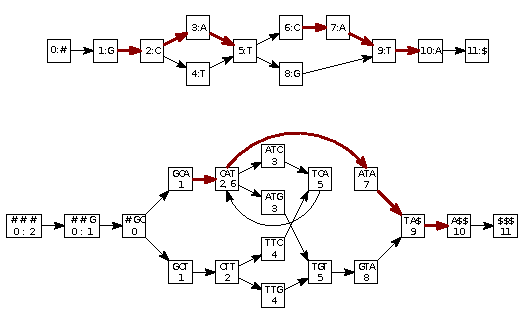
\includegraphics[width=\textwidth]{Chapter2/Figs/sequence_graph_to_DBG.pdf}
  \caption[A sequence graph and its de Bruijn transformation]{
    A sequence graph and its de Bruijn transformation.
    Reprinted from \cite{siren2017indexing}.
  }
  \label{fig:seq_graph_to_dbg}
\end{figure}


This pruned graph is then encoded in a generalization of the FM-index built on a BWT of the $k$-mers in the pruned DBG.
The FM-index is extended to support search over the DBG by adding auxiliary bitvectors which record the indegree and outdegree of nodes in the pruned DBG.
These are used in backwards search to adjust the suffix array ranges that are considered, expanding them when the indegree is greater than 1 and contracting them when the out degree is greater than 1, in effect encoding the graph structure into the index in a space efficient and traversal optimized manner.
The technique is the same as that used in GCSA, although GCSA indexes a reverse deterministic automaton rather than a DBG.
Impressively, GCSA2 uses around 1 bit per $k$-mer in indexes of the 1000GP pangenome graph for $k=128$, which is favorable with comparsion to true DBG indexes, as these need to record information about each $k$-mer that is not important for GCSA2.

As an FM-index like structure, GCSA2 supports queries for a pattern $X$ that yield the suffix array interval matching a given pattern: $find(X) = ( sp_{X}, ep_{X} )$, and $locate( sp_{X}, ep_{X} ) = \{ b_1 \ldots b_{count(sp_{X}, ep_{X})} \}$ which yields the positions in the input VG where the given patterns occur.
The afformentioned LCP array allows the index to support several operations that require a suffix tree, including $count(sp_i, ep_i)$, which returns the number of matches for a given suffix array range, and $parent(sp_i, ep_i) = (sp_j, ep_j)$, which conceptually allows us to traverse the suffix links embedded in the suffix tree and forms the core of maximal exact match (MEM) inference using GCSA2.

\begin{figure}[htbp!]
  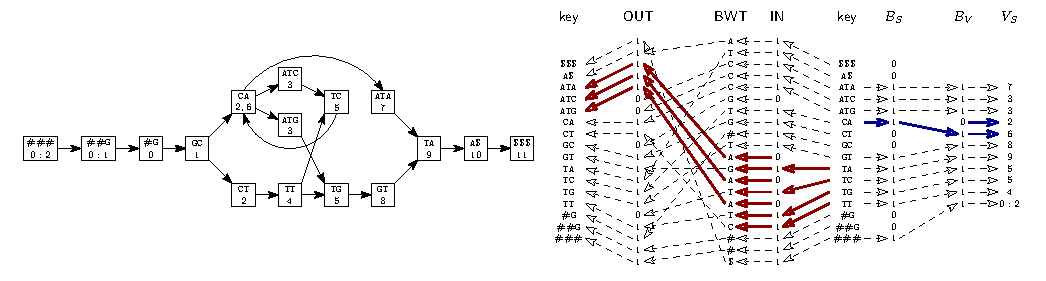
\includegraphics[width=\textwidth]{Chapter2/Figs/DBG_to_GCSA.pdf}
  \caption[Searching in the {\tt GCSA2}]{
    Left: An order-3 pruned de Bruijn graph 3-equivalent to the de Bruijn graph in figure \ref{fig:seq_graph_to_dbg}.
    Right: GCSA for the graph.
    Leftward arrows illustrate backward searching, with the red arrows showing it from {\tt T} to {\tt AT}.
    Rightward arrows mark the samples belonging to each node, with the blue ones showing them for node {\tt CAT}.
    Reprinted from \cite{siren2017indexing}.
  }
  \label{fig:gcsa2_search}
\end{figure}

GCSA2 resolves a number of problems that limit the utility of other graph path indexing schemes.
Indexing a pruned DBG allows GCSA2 to be applied to arbitrary bidirectional string graphs.
It avoids exponential costs during backwards search using the graph augmentation of the FM-index, which is itself supported by the transformation of the input variation graph into a pruned DBG.
However, it does incur exponential costs in indexing, but to mitigate the affects of these it may be constructed mostly in external memory, and furthermore construction may be broken into pieces by chromosome or some other subdivision of the graph.
Its external memory construction algorithm uses a prefix doubling approach to transform an input DBG of order $k$ to one of order $2^mk$ through $m$ doubling steps.
The high-order DBG need never be loaded into RAM but is induced from a lower-order DBG augmented with sufficient positional context on its nodes to support the disk-backed prefix doubling process.
By default, {\tt vg} runs GCSA2 with input $k=16$ and $m=4$, yielding a final DBG with $k=256$.
In indexing a DBG, GCSA2 limits the maximum-length query for which no false-positive results will be returned to the order $k$ of the DBG.
This has the benefit of allowing GCSA2 to index complex graphs, as a shorter $k$ may be chosen to limit exponential costs.
Provided the final alignment is completed against the full VG using DP-based alignment techinques that have non-exponential costs, the DBG input to GCSA2 may be constructed from a VG in which complex regions have been masked or reduced in local complexity using prior information such as a haplotype panel.

To appreciate the costs of indexing a human genome sized graph\footnote{Precise sizes are given later in the discussion of results.}, the order-256 GCSA2 index of the 1000GP variation graph may be constucted using less than 500GB of scratch space, to and from which are written approximately 3TB during construction, all while requiring less than 50G of RAM.
This puts GCSA2 indexing's resource requirements well within the specifications of standard commodity compute servers.
The resulting index occupies between five and ten times the input graph's serialized size, so no more than 50G for something in the order of a human genome.

\subsection{Haplotype indexes}
%*1.5p 3h*
% worth mentioning gpBWT and PBWT
Recording the path set of a graph in XG (described in section \ref{sec:graph_topology_index}) requires $O(N{\cal L}|P|)$ space where ${\cal L}$ is the average haplotype length, $N$ is the number of nodes in the graph, and $|P|$ is the number of paths in the graph.
Although, such a representation can be compressed, the size of this representation will grow linearly with the addition of new paths, making it impractical as a means to record very large numbers of genomes.
This encoding does simplify positional queries, but to do so each path must be stored independently and without reference to other paths.

Recording collections of paths is an important requirement for the use of VG in resequencing, as the Markovian property of the bare sequence graph $G = (N, E, P= \emptyset)$ means it can encode exponentially many paths relative to the true input path set used to build the graph.
This introduces significant issues during read mapping and genome inference.
With increasing variant density the number of haplotypes grows exponentially, and this can lead to spurious mismapping as discussed in section \ref{sec:1000GP_sim}.
The exponential growth of the path space of the graph has relevance for sequence indexing with GCSA2, and as described in \ref{sec:graph_sequence_indexes}, simplification of the graph input to GCSA2 indexing is required to reliably build indexes.
A haplotype index is the only way that the pruning operation applied to the graph may preserve known haplotypes, rather than defaulting to the reference genome in such cases.
Efficient path indexes could be used for many operations in variant calling and phasing, and may have utility in assembly problems, for instance to losslessly record a read set embedded in a squish graph representing their mutual alignment (section \ref{sec:from_pairwise_alignments}).

Haplotypes from the genomes of the same species are often shared exactly, which suggests that they may be very efficiently compressed.
This property was first used to store large haplotype sets in the \emph{positional BWT} (PBWT) \cite{durbin2014efficient}.
As input the PBWT assumes a set of haplotype strings $S_1 \ldots S_m$ of the same length which describe a set of haplotypes relative to a set of variable loci.
$S_j[i]$ records the allele in haplotype $j$ found at locus $i$.
We set $S_j[i] = 0$ when haplotype $j$ has the reference allele at locus $i$, and $S_j[i] > 0$ if it encodes one of possibly several alternate alleles.
The PBWT can be understood as an FM-index of texts $T_1 \ldots T_m : T_j[i] = (i, S_j[i])$ \cite{gagie2017wheeler}.
To search for a haplotype of $h$ in the range $[i,j]$ we look for pattern $h' = (i, h[1]) \ldots (j, h[|h|])$.
The alphabet size of this FM-index is large, but the matrix like structure of the haplotype set means that we can implicitly encode the array indexes by building a separate sub index for each position.
Applying run length encoding to the BWT allows extremely good compression of real haplotype sets.

With the \emph{graph positional Burrows–Wheeler transform} (gPBWT) \cite{Novak2016gPBWT}, we extended this model to work on variation graphs.
The basic model is the same as the generic PBWT except that instead of variant matrix positions we consider haplotype traversals of node ``sides'' $n_i$ or $\overline{n_i}$, and rather than a local alphabet of variant alleles we encode a local alphabet $\Sigma_{n_i} = \{ j \in N | e_{ij} \in E \}$ which describes the set of nodes $n_{\{j \in N | e_{ij} \in E \}}$ to which haplotypes go after the current node (side) $n_i$.
As in the generic PBWT we build an FM-index of $T_1 \ldots T_m$, encoded in what we call the $B_s$ arrays, which provide the local description of prefix sorted haplotypes (equivalently, threads) traversing each node side $n_s$.
To deal with bidirectionality of paths in variation graphs, each haplotype must be encoded in its forward and reverse orientation.
We demonstrated the expected sublinear scaling property for the gPBWT by building an index for chr22 with increasing numbers of samples.
Constructing the gPBWT for large haplotype sets proved difficult when using our particular implementation.
Progressive construction of the gPBWT in generic graphs was enabled by encoding the gPBWT into dynamic succinct data structures and adding a single haplotype thread and its inverse one at a time.
The overheads associated with the dynamic succinct data structures and the linear time required resulted in an infeasible serial construction algorithm for large haplotype sets, and all experiments were carried out using a partially ordered construction algorithm that worked using a VCF file as input.

The \emph{graph Burrows-Wheeler transform} (GBWT) \cite{siren2018haplotype} simplifies the data model used by gPBWT so that it is independent of {\tt vg} and can be applied to generic sequence graphs.
The most generic conceptual model for the GBWT is as the FM-index of a transformation of the graph's paths $p_1\ldots p_m \cup \overline{p_1}\ldots \overline{p_m}$ into the text $T = \$( p1 = n_i\ldots n_j) \ldots \$ (\overline{p_m} = \overline{n_j} \ldots \overline{n_i}) $ wherin the paths are rewritten as a series of characters representing node traversals in a large alphabet and delimited by a marker $\$$.
Unfortunately, this approach is technically challenging to implement due to the extremely large size of $T$ for moderately-sized haplotype sets embedded in variation graphs ($|T| \approx 10^{12}$ for the 1000GP  \cite{siren2018haplotype}).
Serializing the path set during construction is not feasible, which suggests a dynamic version of the model is required.
Also this approach it does not benefit from a number of features which distinguish paths in typical variation graphs.
Sequence graphs based on homology tend to be manifoldly partially ordered, as unique sequence will easily assemble into long coherently-ordered segments.
If we sort the identifier space of these graphs, then most haplotypes passing through the graph will be comprised of increasing or decreasing sequences.
This is even more true for VGs built from VCFs, although even there the issue of indels must be handled in a way that is very different from the assumptions that simplify the PBWT.
The nodes in these regions of the graph will also tend to have low degree.
These features suggest that a local compression of each's node's context in the graph can be achieved very efficiently.
The GBWT can thus benefit from a formulation in similar positional terms as those used in PBWT, with the augmentation of the positional model to record its local context in the graph.
The isolation of each node's context can also allow the construction of the GBWT to be completed in parallel over isolated segments of the variation graph, such as separate chromosomes, and these may be merged easily.

In the GBWT we break the full FM-index into per-node records, each of which encodes a header consisting of a description of the local edge transition alphabet $\Sigma_{n_i}$ through which the graph topology is maintained, and a body $BWT_{n_i}$ which is the subset of the full BWT specific to paths traversing $n_i$.
The GBWT supports essential FM-index operations including: $find(X) \to [sp, ep]$ yielding the lexicographic range of suffixes starting with pattern $X$; $locate(sp, ep) \to$ paths occuring in $SA[sp, ep]$; and $extract(j) \to p_j$ which returns the $j$th path in the graph.
By encoding all paths in both orientations, the GBWT can be treated as a kind of FMD-index for haplotypes, allowing bidirectional search.
In principle, this means that the GBWT turn supports MEM-based haplotype matching, which has potential uses in genotype imputation, phasing, association mapping, and other population genetic and evolutionary assays.

The GBWT representation reflects a number of assumptions that tend to hold for most DNA sequence graphs.
Nodes tend to have low degree, which means the local alphabet size $|\Sigma_i|$ is small and we can afford to decompress a local alphabet encoding efficiently.
Most nodes are not traversed more than once by each path, so the $BWT_{n_i}$ remains small and can be accessed and modified in bounded time.
Due to relatedness among individuals in many species, it is sensible to assume that haplotypes will be highly repetitive, which allows for efficient RLE encoding of $BWT_{n_i}$.
The graph is sorted, and its identifier space has been compacted, which allows us to store the same information for the entire range of node identifiers in bounded memory with respect to $|N|$.
The graph tends to be locally ordered in most cases, which decreases the complexity of recording the graph topology in our records.

\begin{figure}[htbp!]
  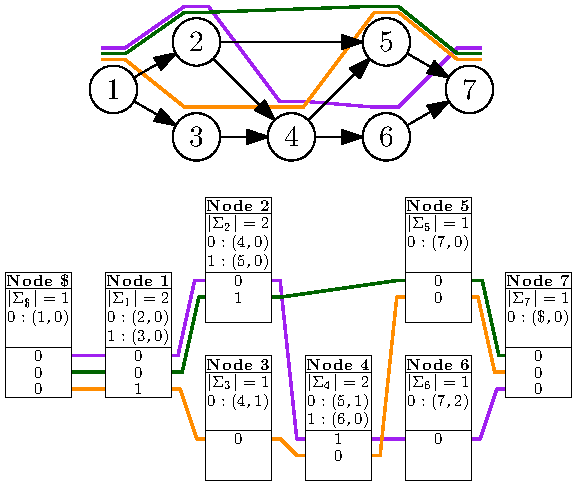
\includegraphics[width=\textwidth]{Chapter2/Figs/gbwt-example.pdf}
  \caption[The Graph Burrows Wheeler Transform]{
    Left: A graph with three paths. Right: GBWT of the paths.
    Reprinted from \cite{siren2018haplotype}.
  }
  \label{fig:gbwt-example}
\end{figure}

A \emph{dynamic GBWT} implementation presents the node records through an index over the range of $[min(i : n_i \in N), max(i : n_i \in N)]$, for each linking to its header, body, incoming edges, and haplotype identifiers.
Construction employs this model in a manner similar to RopeBWT2 \cite{li2014fast}, where batches of paths are insert into the index in a single step following the BCR construction algorithm to build the BWT for large sequence sets \cite{bauer2013lightweight}.
This process includes the new paths in the dynamic GBWT by rebuilding each node record affected by the extension.
At the end of each step the dynamic GBWT remains valid.
When constructed, the GBWT may be encoded in a compacted but immutable form that uses less memory.
By breaking the construction process apart for each chromosome and finally merging the compressed GBWTs, it is possible to build the GBWT for the entire 1000GP haplotype set around 30 hours.
The resulting GBWT requires $\approx 15$GB, with around half allocated to the GBWT structure itself and half to haplotype identifiers.
Incredibly, this structure requires less than 0.1 bits per mapping in the stored paths.
This demonstrates that it has fully exploited haplotype sharing in the 1000GP set, and we can expect that this compression rate will only improve with the addition of more samples.

\subsection{Generic disk backed indexes}
%*0.5p 0.5h*
\label{sec:generic_disk_backed_indexes}
I began the development of {\tt vg} alone, starting with schemas for the data models, then building an index of the graph using the disk-backed key/value store RocksDB\footnote{\url{https://github.com/vgteam/vg/blob/master/src/index.hpp}}.
In principle this would allow working with graphs that were many times larger than main memory.
I transcribed the data model into namespaces and sorted arrays written into the key/value store.
As compressors of various types could be applied to the sorted arrays backing RocksDB, the memory uses of this approach were ultimately similar to those for the final indexing models that I present here.
This encoding included the graph, alignments, and 
However, performance was far worse and the initial version of the aligner based on these systems could not achieve meaningful results using reasonable amountsof time for large graphs.
Ultimately, this flexible database model has remained important for some pipelines, in particular as a technique to organize alignments against the graph.
The ability of a disk backed index to exceed main memory limits makes it useful for exactly this kind of workload.
Unfortunately, other workloads such as sequence queries were untenable for large genomes, with reliable performance only possible if the entire index of spaced $27$-mers were cached in RAM, requiring nearly 200G in the case of the 1000GP variation graph.
The sorted disk-backed array does have the useful property of allowing prefix queries of the $k$-mer set, but this can easily be attained with GCSA2.
Finally, on the networked storage available in my instutitional setting, the construction costs for disk-backed index models were usually much worse than those of the XG and GCSA2 models.

\subsection{Coverage index}
\label{sec:coverage_index}

As variation graphs can remove specific bias towards any particular sequence, they imply a uniform vector space in which all samples can be placed for later analysis.
One reductive form that this can take is a coverage map, which is similar to the labeling required to implement ``colors'' on a DBG.
Here, we lose information about the edge traversals and the paths taken through the graph
In principle, this doesn't matter for many kinds of variation.
And in benefit,, but the complexity of computing the coverage map is linear in the number of the input alignment set, and it requires $O(\sum_{\forall{n_i\in N}}|n_i|)$ space.
In exploration of this, I developed an indexing method that allows us to build and query compact coverage indexes.
Simply, we map the sequence space of the graph into a vector and record coverage across it for a GAM read set.
During construction, a succinct format is employed to store the coverages in a single byte as long as they are below 255, and in a secondary hash table if they reach 256.
Finally a compressed integer vector is generated, which be queried by graph position computed from the XG index of the graph.
I extended this concept with a kind of succinct ``pileup'' format \cite{li2009sequence} generated from the edits against the graph.
In this model edits in mappings which don't match the reference were serialized into a byte alphabet using protobuf, such that each non-reference edit $e_j$ at position $b_i$ was recorded as a string $\$b_i e_j$, and these were combined and delimited by a character $\$$ escaped from the representation by duplication of all instances in the byte string.
By building a CSA/FM-index from these I can obtain the set of edits at each graph position through pattern matching.
However, I found it impossible to construct this for a large high-coverage sequencing sample, and have not continued research into the topic.

\section{Sequence alignment to the graph}
%*0.5p 0.5h*
We have built variation graphs to be used as a pangenomic reference for sequence analysis.
The most important step in such analysis is sequence alignment.
Aside from whole genome alignment methods, which implicitly use such techniques, no previously published approach allows the sensitive alignment of long sequences to large graphs.
The graphs we build are meant to encode any kind of variation.
Our alignment algorithm should be able to represent them in alignments as well.
I have explored a particular hierarchical model of alignment that does by using hierarchical partial alignment of the sequence to the graph.
In \emph{chunked alignment}, large sequences are broken up into overlapping segments, each of which is aligned individually in any order or orientation.
This subdivision provides a kind of banding to the alignment algorithm, preventing the evaluation of the full DP matrix, but more importantly it also allows alignments that are generated to represent any kind of variation.
Each chunk is aligned indepenently using one of several possible algorithms.
I use GCSA2 and the XG index to find and cluster maximal exact matches (MEMs) using a global pseudoalignment algorithm that exploits approximate distance indexes in the graph to drive colinear chaining of MEMs.
The same colinear chaining model, with different parameters, is used to establish the optimal global chain through the alignment chunks, thus yielding a full alignment for the input sequence of any size.
In the simple case where our reads are shorter than the standard chunk size (256bp), the alignment behaves exactly as in {\tt bwa mem}, and this use constitutes much of the application of the method in the subsequent chapter.
Locally, I use a SIMD-accelerated dynamic programming approach that generalizes Smith Waterman Gotoh (SWG) to operate on a graph to align each chunk to each candidate locus.
\emph{Unfolding} and \emph{DAGification} transform a cyclic bidirectional sequence graph with inversions to an acyclic simple sequence graph one in which all $k$-paths in the first graph are represented.
Any alignment algorithm that may be implemented on a sequence DAG can thus be used.
Optionally, other alternative DP alignment algorithms implementing a banded global alignment can be applied, and I also report on these as I have supported their authors' implementation of them in {\tt vg} and used them in related algorithms such as the \emph{surjection} of alignments into a particular reference path.

\subsection{MEM finding}
%*2p 2h*
{\tt vg} can efficiently align reads against large graphs supported by xg and GCSA2 indexes through an alignment process based on maximal exact match sequences between the query sequence and the reference graph.
First, a set of super-maximal exact matches (SMEMs) of a read are generated by traversing the suffix tree encoded in the GCSA2 index until the count of matching strings drops to 0, then backing off one step to find all longest exact matches. 
A recursive series of ``reseed'' passes through the traversal can then identify next-longest matches which are used both to improve sensitivity.
These are not super-maximal, thus we tend to call these heuristically derived exact matches ``MEMs''.
Then, chains of MEMs that are consistent with the query sequence are found using a Markov model in which the optimal alignment is likely to form a Viterbi path.
For each candidate chain, we then locally align the read against the graph. 
Scoring results from the local alignment are used to rank the candidate alignments.
We then return the best alignment, or multiple candidates if multiple mappings are required.

\subsection{Distance estimation}
%*1p 1h*
To cluster our MEMs we require a distance function that returns the minimum distance between any two positions $dist(b_i, b_j) \to \min_{\forall p \in N \times N}{|p|} : pos(p[1]) = b_i \land pos(p[|p|]) = b_j$.
Distance measurement between nodes in a variation graph is non-trivial, with exact solutions to the problem theoretically requiring $O(E \log \log L)$ where $L = \max_{\forall n_i \in N} |n_i|$ is the maximum node length \cite{karlsson1983mlog}.
Precomputation of the full set of distances would thus require $O(N^2 E \log \log L)$ time and $O(N^2)$ space, which is infeasible for any large graph.
Many variation graphs are mostly linear, which we can exploit to build an approximate distance metric.
Provided we have applied a partial sort to the graph, in the partially ordered regions we can use the offset of each node in the XG sequence vector $S_\textbf{iv}$ as approximate 1D coordinates for each node.
We expect that in much of the graph $S_\textbf{bv}^{select_1}(id(b_j)+offset(b_j)) - S_\textbf{bv}^{select_1}(id(n_i)+offset(n_i)) \propto dist(b_i, b_j)$, where $id(b)$ is the function that returns the rank of position $b$'s node in the XG index, and $offset(b)$ returns the position's offset inside the sequence label of the node.
We use this to provide a first order approximate distance metric.
Nonlinearities in the graph will frustrate this metric, and to manage these we rely on the positional index provided by the \emph{positional paths} given in the XG index.
In these, we can query the relative positions of nodes in the path in $O(1)$ time.
Where both positions are not on the same path, we can use local exploration of the graph near our positions $b_i$ and $b_j$ to attempt to find anchoring nodes on the same path.
In our clustering step we can consider the multiple coordinate systems to develop a global pseudoalignment.

\subsection{Collinear chaining}
%*0.5p 0.5h*
\label{sec:collinear_chaining}

If the MEMs do not cover the full read length then we attempt to link them together into chains by building a Markov model in which the best possible chains form high-scoring paths. 
In this model the nodes correspond to the reference graph positions where MEMs in the read occur and the transitions between nodes correspond to a weight that is proportional to the indel size implied by the difference in distance between the positions of the MEMs in the read and their approximate or embedded path-relative distances in the graph. 
To consider the coordinate spaces implied by all applicable embedded paths, we record one node per embedded path that each MEM touches. 
We also record a node for each MEM based on its approximate position in the graph, which is estimated as its position in the concatenated nodes of the partially sorted graph. 
If we are aligning a read pair, the weight between MEMs on different fragments is proportional to the probability of that distance under a learned model of the fragment distribution. 
One we establish this model, we take the Viterbi path through it as our first candidate alignment. 
By masking this path out and re-running the Viterbi algorithm on the model, we can extract a series of candidate alignments in descending order of goodness. 
This clustering model implements a kind of co-linear chaining such that optimal chains are made of series of MEMs which have similar spacing in the read and in the reference system into which we are mapping the read. 
Although the exact algorithm is different, in spirit our implementation is similar to that developed in \cite{kuosmanen2018using}, which extends colinear chaining to DAGs by running a similar model over the paths in a minimum path cover which they efficiently compute on the graph.

\subsection{Unfolding}

Every node has an implicit default orientation (see Graph Representation below) so that it is possible to determine edges that cause an inversion, i.e. those which connect between a forward and a reverse complement node orientation. 
In {\tt VG::unfold} we use a breadth first search starting at every inverting edge in the graph to explore the reverse complemented portions of the graph that we can reach within length $k$ from the inverting edge.
We then copy this subgraph, take its reverse complement, and replace the inverting edges connecting it to the forward strand of the graph with non-inverting ones.
If $k$ is greater than any length in our graph, then we are guaranteed to  duplicate the entire reverse complement of the graph on the forward strand, effectively doubling the size of the graph if we have any inversions in it.%, as shown in Supplementary Figure 3. %\ref{fig:unfold}.

\subsection{DAGification}
\label{sec:DAGify}

Variation graphs may have cycles.
These are useful as compact representations of copy number variable regions, and arise naturally in the process of genome assembly.
However, our partial order alignment implementation does not handle these structures, and so when they occur we convert them into an $k$-path equivalent acyclic graph in order to align with DAG-based alignment algorithms.
To do so, we unroll cyclic structures by copying their internal nodes an appropriate number of times to allow a given query length to align through the unrolled version of the component.
In this graph, we can find all paths of length $k$ found in the original graph.
If our query is shorter than this limit, $k \geq |Q|$, then we are guaranteed to find the optimal alignment in the original graph by aligning against the DAGified one.

We first detect all strongly connected components by using a recursion-free implementation of Tarjan's strongly connected components algorithm \cite{tarjan1972depth}.
Then, we copy each strongly connected component and its internal edges into a new graph.
We greedily break edges in this graph that introduce cycles.
Next we k-DAGify the component progressively copying the base component and, for each edge between nodes in the component, connecting from the source node in the previous copy to the target node in the current copy.

We use dynamic programming to track the minimum distance back through the graph to a root node outside the component at each step.
When this reaches our target $k$, we stop unrolling, and add the expanded component back into the graph by reconnecting it with its original neighborhood.
For each copy of a node in the DAG-ified component we copy all its inbound and outbound edges where the other end of the edge lies outside the strongly connected component.
The resulting graph is acyclic and supports queries up to length $k$ on the original graph using the translation that we maintain between the new graph and the source one.
%Figure \ref{fig:kdagify} 
%Supplementary Figure 4 provides a visual description of the process.


\subsection{POA and GSSW}
%*2p 2h*

Partial order alignment (POA), which I previously describe in section \ref{sec:MSA}, generalizes string to graph and graph to graph alignment for the case of sequence DAGs.
It is the core alignment algorithm used in {\tt vg map}.
Where POA was defined for graphs in which each node represents a single base, we must account for the compressed nature of variation graphs, which adds some complexity in our definition and implementation.
Furthermore, default POA is efficient in terms of runtime, but does not benefit from vectorized instructions that are now ubiquitous on modern processors.
As part of work in the 1000GP, I developed an accelerated version of POA which I will present in detail here.

Given a candidate cluster of exact matches that we have extracted from the MEM chaining model described in the previous section \ref{sec:collinear_chaining}, we want to derive a complete description of the alignment of the read to the reference graph.
Sensitive alignment of each candidate is essential for distinguishing the optimal alignment.

We transform seed chains into alignment using local alignment based on dynamic programming. 
To make this efficient we extended an implementation \cite{zhao2013ssw} of Farrar's SIMD-accelerated striped Smith Waterman (SSW) algorithm \cite{farrar2007striped}, which we term \emph{graph striped Smith-Waterman} (GSSW)\footnote{\url{https://github.com/vgteam/gssw}}.
Single-Input Multiple-Data (SIMD) instructions allow vectorized mathematical operations in a single machine instruction, and can be used to greatly speed up algorithms which can be implemented in terms of operations on vectors.

GSSW generalizes all aspects of SSW to operate over sequence directed acyclic graphs, including affine gap penalties, and retains its matrices for traceback\footnote{SSW discards these matrices for performance reasons, instead establishing the traceback later with local banded DP.}.
This is simple to accomplish if the reference is a graph, as the striping of SIMD calculations in SSW across the reference is done by a single character at a time, and thus boundaries between nodes do not split the SIMD embedded variables.
We can generalize SSW to GSSW by extending the recurrence relation that defines the scores in the DP matrices to consider all previous positions on all nodes that connect to the current one.

Given a query $Q$ and a sequence graph $G = (N, E)$ with sequence length $L=\sum_{i}^{|N|} |seq(n_i)|$.
We record the maximum scores of alignments between $Q$ and $G$ in the tensor $\hat{\cal H} = {\cal H}_1 \ldots {\cal H}_{|N|} :$ each ${\cal H}_i$ is a $|seq(n_i)| \times |Q|$ matix.
$\hat{\cal H}$ thus contains $|Q|\times L$ cells, and when we have completed the scoring phase of alignment each will record the maximum score of an alignment between $Q$ and $G$ ending at $(n_i[x], Q[y])$ in ${\cal H}_{i}[x,y]$\footnote{Here I will use brackets $[\ldots]$ to identify the cells in 2-dimensional arrays.}.
To develop our scores, we use a scoring function $score(a, b)$, which in the case of DNA returns the value of a match (typically a positive integer) when $a = b \lor a = N \lor b = N$ and the value of mismatch when $a \neq b$ (typically a negative integer).
We score a gap beginning with $\omega_\textbf{open}$ and a gap extension as $\omega_\textbf{extend}$
We record the score of a gap along $G$ in tensor $\hat{\cal E} = {\cal E}_1 \ldots {\cal E}_{|N|}$ and a gap along $Q$ in tensor $\hat{\cal F} = {\cal F}_1 \ldots {\cal F}_{|N|}$.

Gaps in $\hat{\cal E}$ extend across the graph, and so we need to consider all the inbound edges when we are at the beginning of a node:

\begin{equation}
  {\cal E}_i[x,y] = \max
  \begin{cases}
    {\cal E}_i[x,y-1] - \omega_\textbf{extend} \\
    {\cal H}_i[x,y-1] - \omega_\textbf{open} \\
    \max_{\forall j : \exists e_{ji} \in E} {\cal E}_j[|n_j|,y-1] - \omega_\textbf{extend} & \text{if } x = 1 \\
    \max_{\forall j : \exists e_{ji} \in E} {\cal H}_j[|n_j|,y-1] - \omega_\textbf{open} & \text{if } x = 1 \\
  \end{cases}
\end{equation}

However, this is not the case for $\hat{\cal F}$, whose data dependencies flow vertically over the query $Q$:

\begin{equation}
  {\cal F}_i[x,y] = \max
  \begin{cases}
    {\cal F}_i[x-1,y] - \omega_\textbf{extend} \\
    {\cal H}_i[x-1,y] - \omega_\textbf{open} \\
  \end{cases}
\end{equation}


The score in $\hat{\cal H}$ combines the affine gap calculations in $\hat{\cal E}$ and $\hat{\cal F}$.
As with $\hat{\cal E}$, we here we also must consider the inbound nodes:

\begin{equation}
  \label{eqn:gssw_h}
  {\cal H}_i[x,y] = \max
  \begin{cases}
    0 \\
    {\cal E}_i[x,y] \\
    {\cal F}_i[x,y] \\
    {\cal H}_i[x-1,y-1] - score(Q[x], n_i[y])\\
    \max_{\forall j : e_{ji} \in E} {\cal H}_j[|n_j|,y-1] - score(Q[x], n_j[y]) & \text{if } x = 1 \\
  \end{cases}
\end{equation}

The values of ${\cal H}_i$, ${\cal E}_i$, and ${\cal F}_i$ are 0 when $x < 1$ or $y < 1$ and node $n_i$ has no inbound edges.
Note that this is the initial condition provided by Gotoh to improve the algorithm of Smith and Waterman.

We fill the matrices using Farrar's SSW algorithm \cite{farrar2007striped}, based on Zhao's implementation \cite{zhao2013ssw}.
By storing the full score matrices we can then trace back from the maximum score in $\hat{\cal H}$ to obtain the optimal alignments under our scoring parameters.
The traceback can be represented as moves in the matrix, or equivalently as the alignment object model described in section \ref{sec:alignments}.

To interface with GSSW we transform a local region of our graph so that it is acyclic and only represents a single strand of the DNA as described in section \ref{sec:DAGify}.
The two operations we use in this transformation are \emph{unfold}, which expands the graph to include its reverse complement where accessible via an inversion, and \emph{dagify}, which unrolls strongly connected components of the graph far enough that we are guaranteed to be able to find any sequence of given length $k$ in the source graph in the unrolled one.
This allows us to align any sequence of up to length $k$ against a completely general section of a variation graph.
Through these steps we retain a mapping from old node ids to new ones, which we will use to project alignments to the transformed graph back into our base coordinate space.

\subsection{Banded global alignment and multipath mapping}
\label{sec:banded_global}

By modifying equation \ref{eqn:gssw_h} so that it is no longer capped at 0 and changing the traceback so that it goes from beginning to end of query $Q$ and graph $G$, we obtain a ``global'' alignment algorithm with the same properties as Needleman-Wunsch.
The SIMD-based approach of GSSW is not adapted to negative scores, and so the implementation of global alignment to the graph is completed a standard DP approach as in POA.
However, it may be \emph{banded} so that only a limited region of the DP tables need to be explored.
This approach, as implemented in {\tt vg} by Jordan Eizenga, forms the basis for multipath mapping, in which alignments are represented probabilistically as DAGs rather than linear series of node traversals and edits.
In multipath mapping, regions between MEMs in a particular cluster may be aligned using global alignment, so as to obtain full-length descriptions of the alignment in the non-matching region.
Multiple traceback allows for alternatives to be included, and each of these may be scored on the basis of both alignment score and haplotype matching score.
His implementation is key to the development of haplotype aware mapping, which is the subject of a paper currently in development by collaborators on the {\tt vg} project.
In the case of low-error reads, this limited exploration of the DP problem allows for fast derivation of the optimal alignments, and so the multipath mapper in {\tt vg mpmap} achives runtime comparable to or exceeding the simpler algorithm in {\tt vg map}.
It is also important to mention here as it forms the basis for alignment surjection, in which an alignment to the graph is projected into the linear reference.

\subsection{X-drop DP}

As our query length $|Q|$ increases, so does the practical complexity of deriving the alignment using POA/GSSW.
Given that we tend to align against proportionally larger graphs and so we effectively face a quadratic penalty with increasing alignment length, $|Q| \propto |L| \implies$ GSSW is $O(|Q|^2)$.
The most direct solution to this is to use a banded alignment method like banded global alignment, as described in section \ref{sec:banded_global}.
However, this method cannot exploit data parallel operations that allow dramatic speedups on modern processors.

In the course of our work on {\tt vg}, Eizenga and I explored the application of Hajime Suzuki's adaptive banded global alignment (libgaba)\footnote{\url{https://github.com/ocxtal/libgaba}} \cite{suzuki2017acceleration}, which has been used in to greatly improve alignment speed with long single-molecule reads \cite{li2018minimap2}.
In this approach, an antidiagonal band of cells are computed at each step, of a predetermined width designed to fit into the word sizes of SIMD instructions.
The band can move either ``right'' or ``down'' at each step, depending on where the highest score is found.
A termination criteria is given, so that alignment stops when the maximum score falls a given amount.
This is similar to the X-drop parameter used in BLAST to stop alignment extension.
Although it improves performance it can hurt sensitivity to indels.

Suzki had already implemented a version alignmen over graphs by transforming the graph into a tree through a dynamic unrolling process akin to that described in \ref{sec:DAGify} and aligning to the tree using libgaba\footnote{\url{https://github.com/ocxtal/comb}}.
His implemenation supports graph to graph alignment as described in section \ref{sec:translation}, but the exponential expansion of the alignment problem is fundamentally limiting.
Eizenga, Suzuki and I discussed methods to merge the bands together after traversal of unifications in the graph, but we could not establish a safe generic method to merge them.
Furcated bands may only be merged directly if they map to the same query coordinate.
This is unlikely to happen if the different paths in the graph that they have traversed have different lengths or if there are apparent indels in the alignment.

During a biohackathon meeting in Kyoto, Suzuki presented an alternative banding model based on the ``X-drop DP'' algorithm from BLAST.
In this model, the alignment is matrix broken into vertical non-striped windows that tile across the DP matrices over fixed subsequences in the query.
To efficiently resolve the data dependencies between successive steps, a SIMD shuffle operation is applied to the cell values stored in each window.
Forward progression of each window stops when the highest score in the forefront cells drops $X$ from the previously-observed maximum.
This approach thus allows the band to spread as wide as needed to accomodate larger insertions, but can be parameterized through the modification of the $X$-drop parameter.
The result is an approach that is more sensitive than the antidiagonal banded alignment in libgaba, but runs a factor of 2 slower for equivalent band sizes.

I have since worked with Suzuki to integrate his implementation of this algorithm \emph{dozeu}\footnote{\url{https://github.com/ocxtal/dozeu}} into {\tt vg}.
Due to difficulties in handling paired end rescue, the approach is not yet performing as well as GSSW for {\tt vg map}.
This remains a work in progress, but is a promising approach to enable the direct alignment of long sequences against the graph.
It is orthogonal to the ``chunked'' alignment approach which I implemented and describe in section \ref{sec:chunked_alignment}.
In principle they can be applied together to build a SV-aware, chunked and banded alignment process.
Future work in this direction may yield a new VG alignment algorithm, but this lies outside the scope of this thesis.

\subsection{Chunked alignment}
%*1p 1h*
\label{sec:chunked_alignment}

For very long reads, where in the worst case the local dynamic programming can become prohibitively expensive, we break the reads into ``bands'' of a fixed width $w$ (default 256 base pairs) with overlap between successive bands of $w/8$.
We align these bands independently, trim the overlaps from the alignments, and build a Markov model from them similar to that built for MEM chaining, 
%\ref{sec:seedchain}, 
only that here we consider sub alignments as nodes in the model rather than MEMs. 
In this model we put weights on transitions between alignments that relate to the estimated distance between the alignments in the graph versus their distance in the read, with the objective of making long co-linear chains be the highest-scoring walks through the Markov model.
We take the viterbi path through the model to be the first-best alignment.
Then, we mask out this path, re-score, and take the viterbi path to get the 2nd, 3rd, and ultimately $N$th best alignment, where we want to obtain multiple alignments. 
After they have been extracted from the model, alignments are ``patched'' using local alignment of unaligned regions anchored in the graph near the end of previous mapped regions, so that sub-alignments which may have been misaligned due to repeats may be locally aligned correctly.
This model allows {\tt vg} to map noisy reads of arbitrary length, and is used as a core component in the long read progressive assembler {\tt vg msga}.


\subsection{Alignment surjection}

Alignments to graphs that include linear reference sequences as paths can be transformed into alignments against those paths.
To be well-defined, this lossy transformation, \emph{surjection}, requires that the alignment path matches the reference path for some portion of their length.
The simplest surjection technique extracts the reference path region matching an alignment and realigns the read against it.
Doing so without global alignment will often result in soft clipping, such as where non-reference alleles in the graph have allowed full length alignment.
This can be resolved to some extent by applying global alignment of the alignment query sequence against the reference.
But a more rigorous approach rebuilds the alignment in parts.
For each piece that is not aligned to the reference, we extract the intervening reference sequence and align only the subset of the query that is no longer matching to this region.
A kind of anchored semi-global alignment may be used on the ends of the reads, where the opposite reference-matching end is not defined.
The resulting alignment to a graph built only from a particular reference path may easily be expressed in the BAM format and thus used by downstream variant calling and analysis methods.

\subsection{Base quality adjusted alignment}
%*2p 2h*

Base qualities are typically reported on the Phred scale so that the probability of error for a given quality $Q$ is $\epsilon = 10^{-Q/10}$. Assuming no bias in which bases are mistaken for each other, this defines a posterior distribution over bases $b$ for a base call $x$.

\begin{align}
    P(b|x, \epsilon) = \begin{cases}
        1 - \epsilon & b = x \\
        \frac{1}{3} \epsilon & b \neq x
    \end{cases}
\end{align}

We use this distribution to derive an adjusted score function. Normally, the match score for two bases is defined as the logarithm of the likelihood ratio between seeing two bases $x$ and $y$ aligned and seeing them occur at random according to their background frequencies. 

\begin{align}
    s_{x,y} &= \log\left(\frac{p_{x,y}}{q_y q_x} \right) \label{eqn:base_score}
\end{align}

Next we marginalize over bases from the posterior distribution to obtain a quality adjusted match score.

\begin{align}
    \tilde s_{x,y}(\epsilon) &= \log\left(\frac{(1 - \epsilon)p_{x,y} + \frac{\epsilon}{3}\sum_{b \neq x}p_{b, y}}{q_y\left((1 - \epsilon)q_x + \frac{\epsilon}{3}\sum_{b \neq x}q_b \right)} \right)
\end{align}

{\tt vg} works backwards from integer scoring functions to the probabilistic alignment parameters in this equation. After doing so, the match scores are given by

\begin{align}
    \tilde s_{x,y}(\epsilon) &= \frac{1}{\lambda} \log\left(\frac{(1 - \epsilon)q_x q_y \exp \lambda s_{x,y} + \frac{\epsilon}{3}\sum_{b \neq x}q_b q_y \exp \lambda s_{b,y}}{q_y\left((1 - \epsilon)q_x + \frac{\epsilon}{3}\sum_{b \neq x}q_b \right)} \right).
\end{align}

Here, $\lambda$ is a scale factor that can be computed from the scoring parameters, and the background frequencies $q_x$ are estimated by their frequency in the reference graph. Since base quality scores are already discretized, the adjusted scores can be precomputed and cached for all reasonable values of $\epsilon$. 

\subsection{Mapping qualities}

The algorithm for mapping qualities in {\tt vg} is also motivated by a probabilistic interpretation of alignment scores.
The score of an alignment $A$ of two sequences $X$ and $Y$ is the sum of scores given in equation \ref{eqn:base_score}.
This makes it a logarithm of a joint likelihood ratio across bases, where the bases are assumed independent (a more complete justification including gap penalties involves a hidden Markov model, but it can be shown to approximate this formula).
We denote this score $S(A|X,Y)$.
Thus, assuming a uniform prior over alignments, we can use Bayes' Rule to motivate a formula for the Phred scaled quality of the optimal alignment, $\hat A$.

\begin{align}
\begin{split}
    Q(\hat A|X,Y) &= -10\log_{10}(1 - P(\hat A|X,Y)) \\
    &= -10 \log_{10}\left(1 - \frac{P(X,Y|\hat A)}{\sum_{A}P(X,Y|A)} \right) \\
    &= -10 \log_{10}\left(1 - \frac{\exp \lambda S(\hat A|X,Y)}{\sum_{A}\exp \lambda S(A|X,Y)} \right) \label{basicqualityscore}
\end{split}
\end{align}

Using the close approximation of the LogSumExp function by element-wise maximum, there is a fast approximation to this formula that does not involve transcendental functions.

\begin{align}
    Q(\hat A|X,Y) &\approx \frac{10\lambda}{\log 10}\left( S(\hat A | X,Y) - \max_{A \neq \hat A}S(A| X,Y)\right)
\end{align}

In practice, we do not compare the optimal alignment to all possible alignments, but to the optimal alignments from other seeds. Thus, the mapping quality indicates the confidence that we have aligned the read to approximately the correct part of the graph rather then that the fine-grained alignment in that part of the graph is correct. It is also worth noting that since this formula is based on alignment scores, it can incorporate base quality information through the base quality adjusted alignment scores.


\section{Visualization}

It is impossible to understand variation graphs without visualization.
While text-mode renderings are sufficient for understanding results in resequencing against the linear reference, this is simply impractical when the reference is a graph.
A set of dotplots can allow us to understand the relationship between many paths embedded in a graph.
But this scales quadratically with the number of embedded paths and quickly becomes impossible to interpret.
The only reasonable solution is to render graphs visually using a coherent set of visual motifs.
If this language can capture the full information in the graph then it can yield complete understanding of small graph regions.
Here I describe several such techniques designed specifically for variation graphs.
The simplest leverage standard utilities for graph drawing, and the most performant of these are hierarchical models that benefit from linear ordering which is often available in reference-ordered variation graphs.
Force-directed layouts techniques developed for assembly graph interpretation allow us to interrogate larger-scale graphs.
Thus far none encode paths, and these are thus lossless with respect to variation graphs.
While it may be topologically complex, any graph is composed of sets which can be ordered linearly.
By exploiting a linear sort of the graph I provide a linear-time layout algorithm that will scale to arbitrary data scales, allowing the visualization of both paths and read coverages against any graph.

\subsection{Hierarchical layout}
%*0.5p 0.5h*

To develop a visualization method quickly, I relied most heavily on the four-phase hierarchical graph layout algorithm {\tt dot} \cite{gansner1993technique} that is part of the Graphviz package \cite{gansner2000open,ellson2001graphviz}.
This approach heuristically attempts to generate a layout in which hierarchical structures in the graph are exposed, visual anomalies such as edge crossings and sharp edge bends are avoided, edges are short, and the layout is overal balanced or symmetric.
It first uses a partial sort on the graph to derive a rank for each node.
This aspect of the algorithm means it is most tenable when used on DAGs.
Then the unordered regions of the partially sorted graph are ordered to reduce edge crossings.
Finally, the actual layout is derived and splines are drawn to show edges.
The output of {\tt dot} as well as other tools in Graphviz is a vector graphic, so the resulting renderings may be viewed in a number of ways.
This allows us to view rather large chunks of graphs, up to tens of kilobases, provided the graph is partially orderable.

To generate a visualization that captures the structure of the variation graph, I transform the graph into a visualization oriented structure in which the graph paths are rendered as nodes and edges.
The layout is then driven entirely by the chosen algorithm in Graphviz, which is typically {\tt dot}.

The set of nodes may be rendered as boxes labeled by $id(n_i)$ and $seq(n_i)$.
The edges have four types, and to indicate these we use the top and bottom of the node boxes.
The top left corner of each node $n_i$ receives incoming edges $e_{ji} \forall j : e_{ji} \in E$.
While the bottom right corner of each node box represents edges arriving at $\overline{n_i}$ and thus $e_{j\overline{i}} \forall j : e_{j\overline{i}} \in E$.
Similarly, the top right corner of each node box represents edges leaving $n_i$, and we add an edge for each $e_{ij} \forall j : e_{ij} \in E$.
Finally, the bottom left corner represents the ``end'' of the reverse complement of the node $\overline{n_i}$, and, so we add edges for $e_{\overline{i}j} \forall j : e_{\overline{i}j} \in E$.
As each edge implies its own reverse complement, we tend to replace edges $e_{\overline{ij}}$ with $e_{ji}$, and this is done both in normalization as in Graphviz based rendering.

Paths are not naturally supported in the Graphviz data model, and must be added as subgraphs with a different rendering style to identify them.
In order to achieve a visually meaningful layout, these subgraphs must be also anchored appropriately into the graph.
For each path, I hash the path name $name(p_i)$ into a set of colors and unicode emoji, yielding $8 \times 766 = 6128$ possible color/symbol combinations.
This generates a symbol for each path that is unlikely to collide with another given the typical application rendering a graph with tens of embedded paths.
The hashing process also ensures the same rendering is returned as long as the same VG (and path names) are given.
For each mapping $m_i\ldots m_{|p_j|} \in p_j$ I add invisible edges to the graph that link the mapping to the particular node it maps to as well as a visible edge in the path color from $m_{i-1} \to m_i$ when $i > 1$ and from $m_i \to m_{i+1}$ when $i < |p_j|$.
A hint is given to {\tt dot} to force the rank of each mapping to be the same as the node it maps to.
Otherwise, the invisible edges encourage {\tt dot} to render the path mappings close to the node they refer to.
The resulting layout tends to look like a kind of multiple alignment matrix, as can be seen in figure \ref{fig:vg_view_dot}.

\begin{figure}[htbp!] 
\centering    
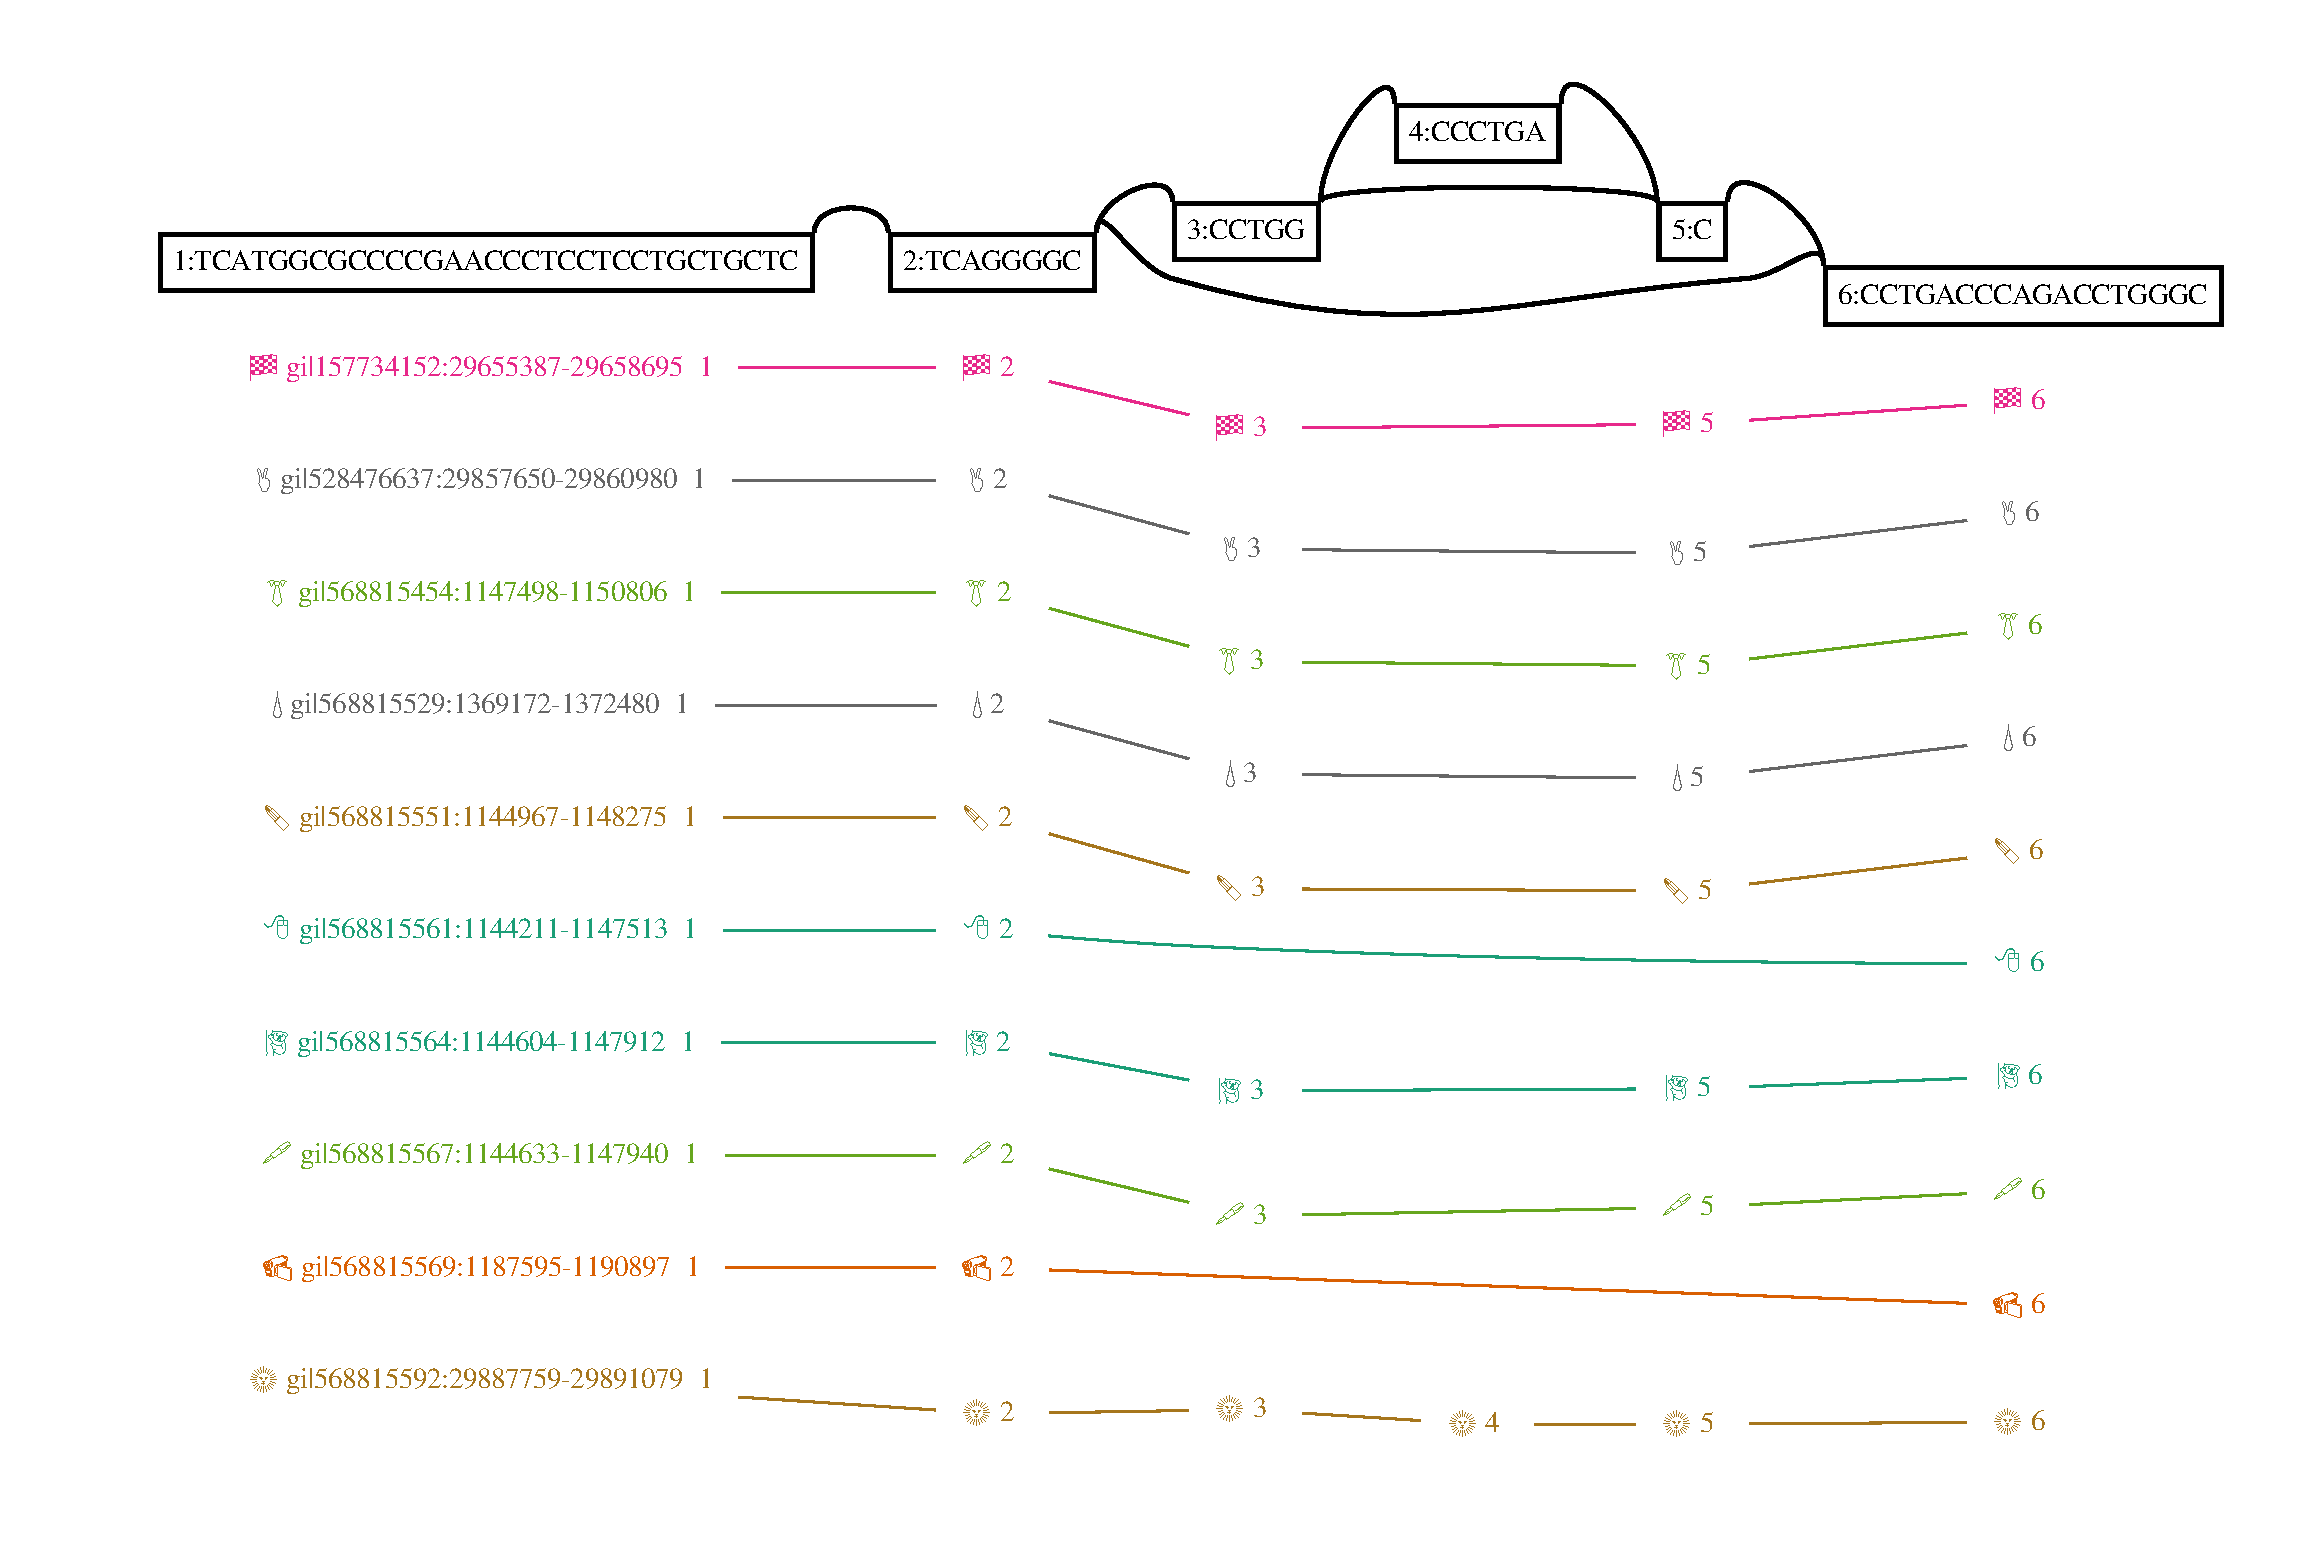
\includegraphics[width=1.0\textwidth]{Chapter2/Figs/vg_view_dp_H-3136_dot.pdf}
\caption[Hierarchical visualization with Graphviz's {\tt dot}]{The beginning of a variation graph built by progressive assembly of the GRCh38 haplotypes in HLA gene H-3136 visualized using {\tt dot}.}
\label{fig:vg_view_dot}
\end{figure}

\subsection{Force directed models}
%*1p 1.5h*

Not all graphs yield easily to hierachical layout algorithms.
Graphviz also includes a force-directed layout algorithm {\tt neato} that simulates the layout which would occur if connected nodes ``pull'' each other together and non-connected nodes ``repel'' each other apart.
While the same input to {\tt dot} may be used with {\tt neato}, in practice the node labels become impossible to read and the edge types are confusing to infer, so a simplified rendering is produced without specific sequence labels on the nodes.
This can still capture the overall structure of the graph as seen in figure \ref{fig:vg_view_neato}.

\begin{figure}[htbp!] 
\centering    
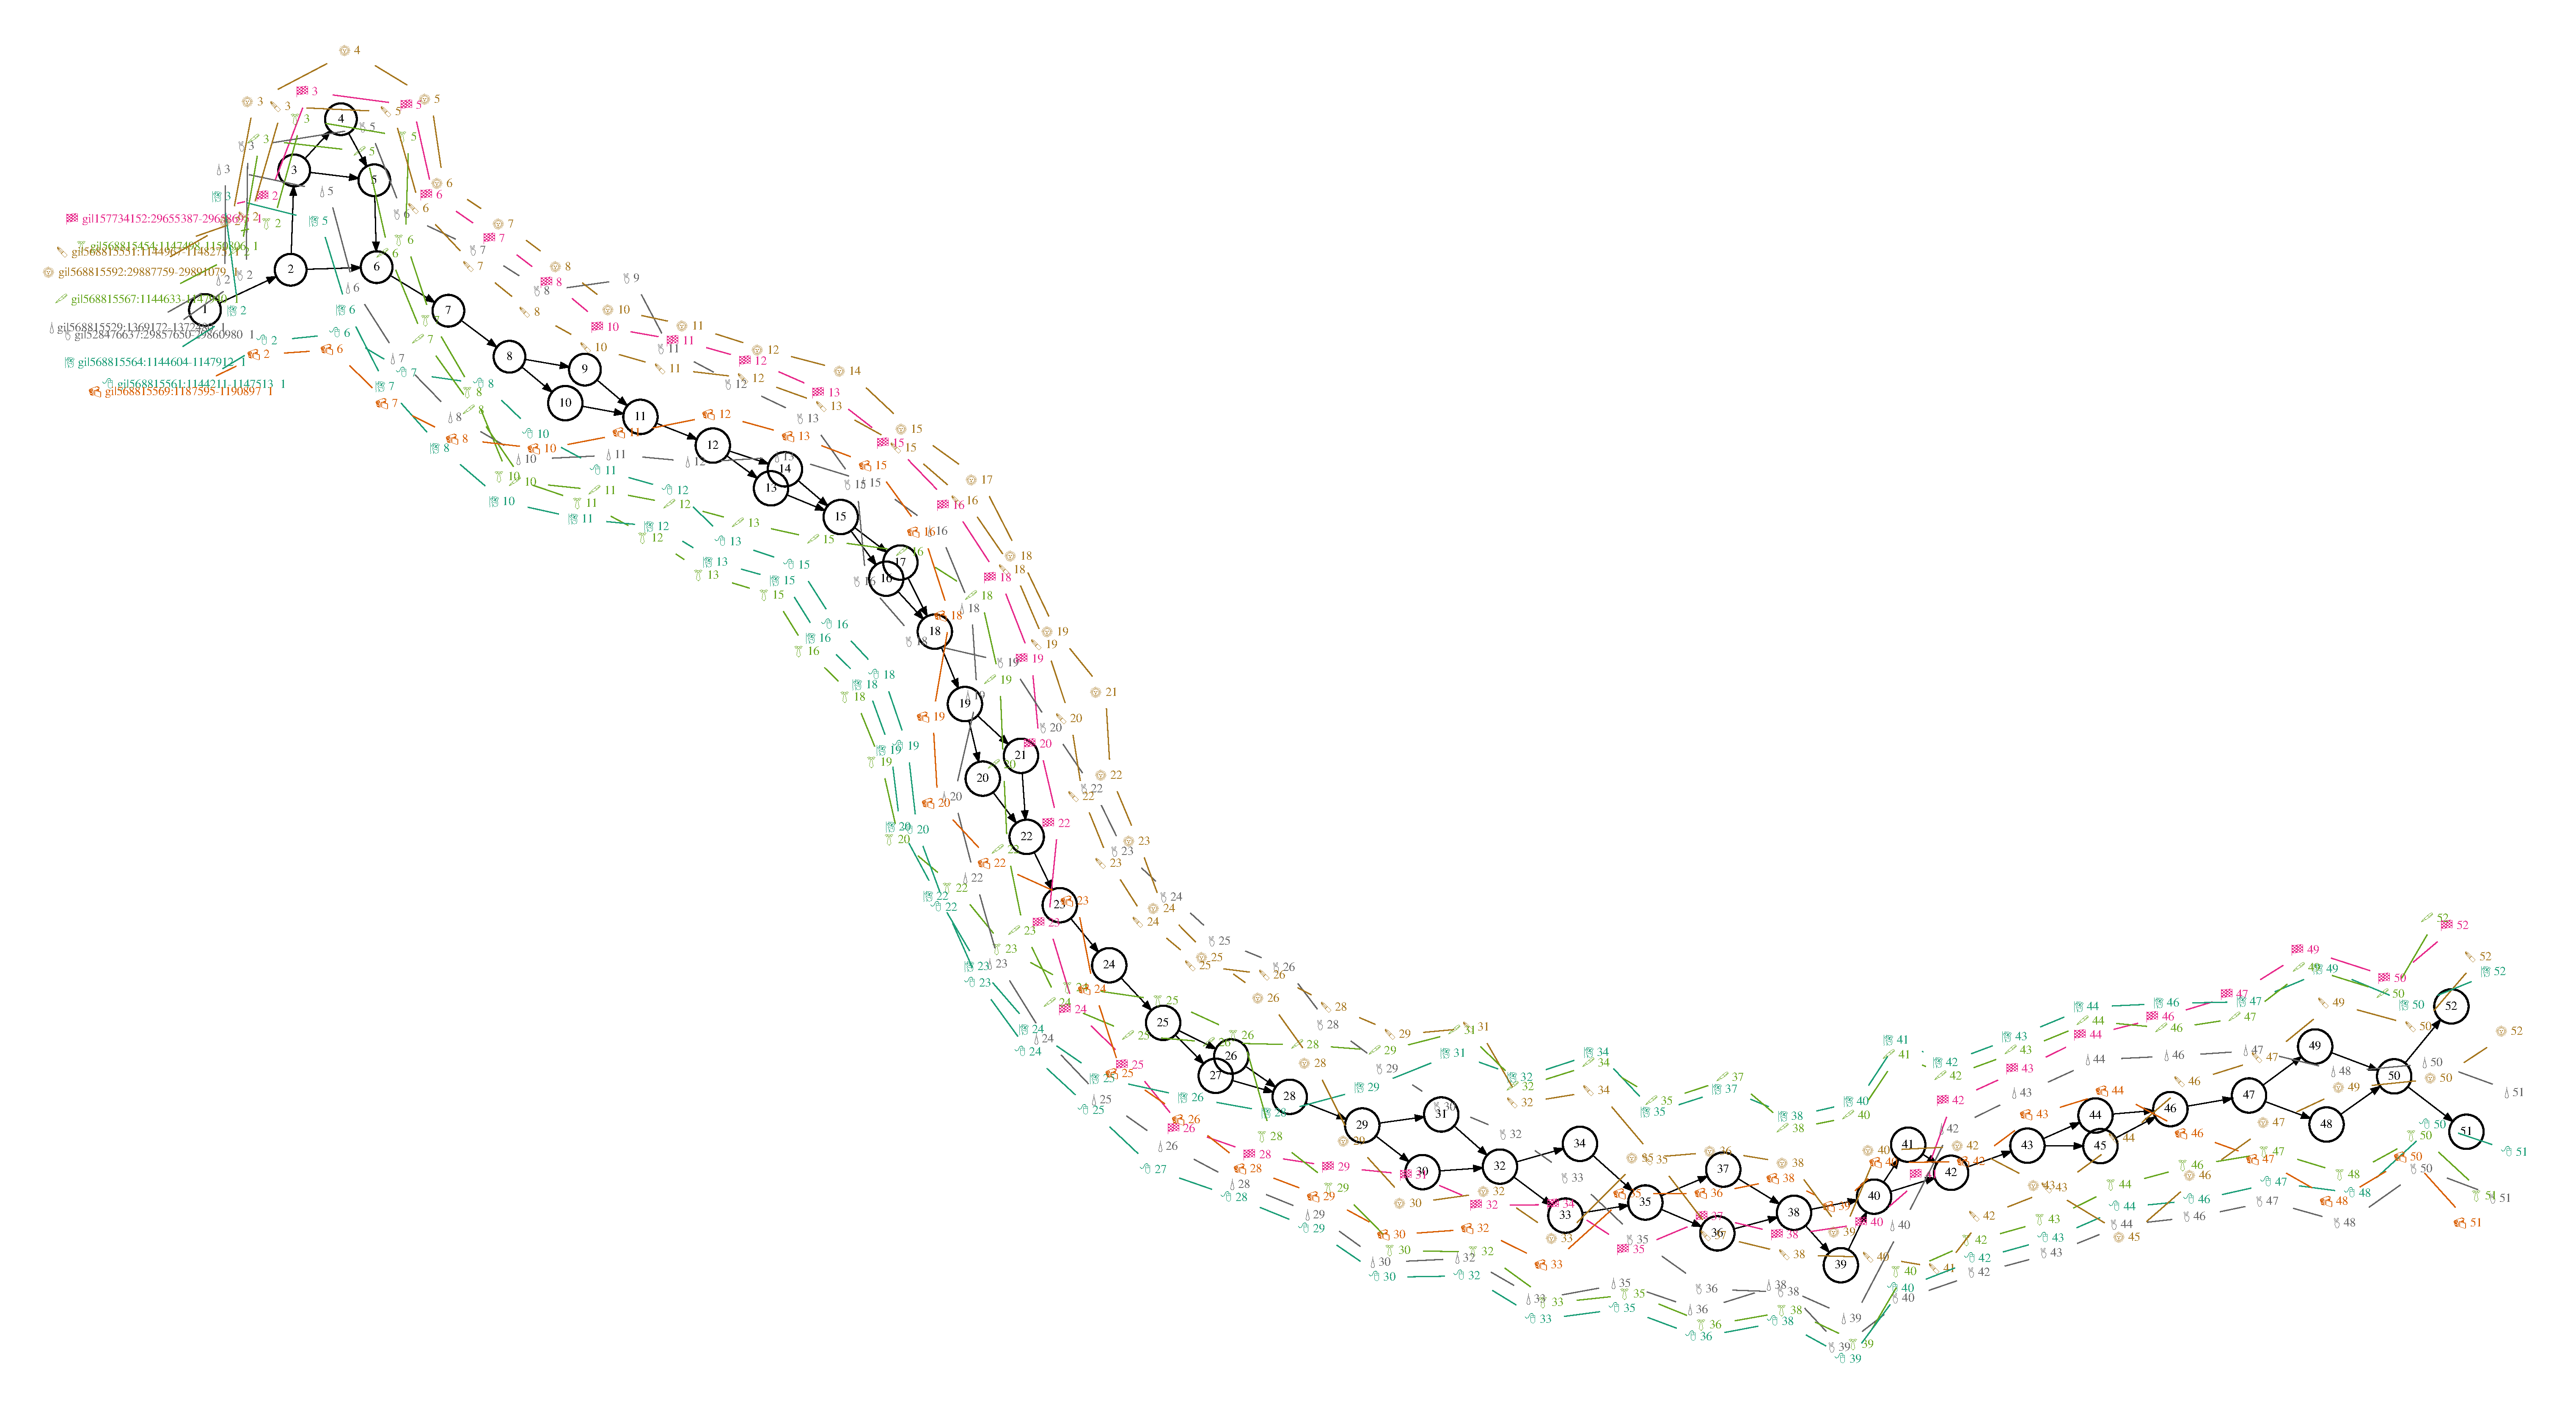
\includegraphics[width=1.0\textwidth]{Chapter2/Figs/vg_view_dpS_H-3136_neato.pdf}
\caption[Force-directed layout with Graphviz's {\tt neato}]{A larger region of the same variation graph in figure \ref{fig:vg_view_dot} rendered using {\tt neato}.}
\label{fig:vg_view_neato}
\end{figure}

While this rendering captures the path space of the graph even in arbitrary graphs, it cannot scale to graphs of significant size due to its approximately $O(|N|^3)$ scaling.
The largest graphs I have used this method to visualize contain tens of kilobases of sequence.
{\tt Bandage} \cite{wick2015bandage} is an alternative method which is oriented towards visualizing assembly graphs.
It reads GFA as input and provides an interactive rendering of the graph topology.
This assembly graph oriented approach allows for much better scaling for rendering variation graphs, and graphs of up to tens of megabases may be rendered.
Figure \ref{fig:vg_view_bandage} shows the properties of this technique using the same region of H-3136.

\begin{figure}[htbp!] 
\centering    
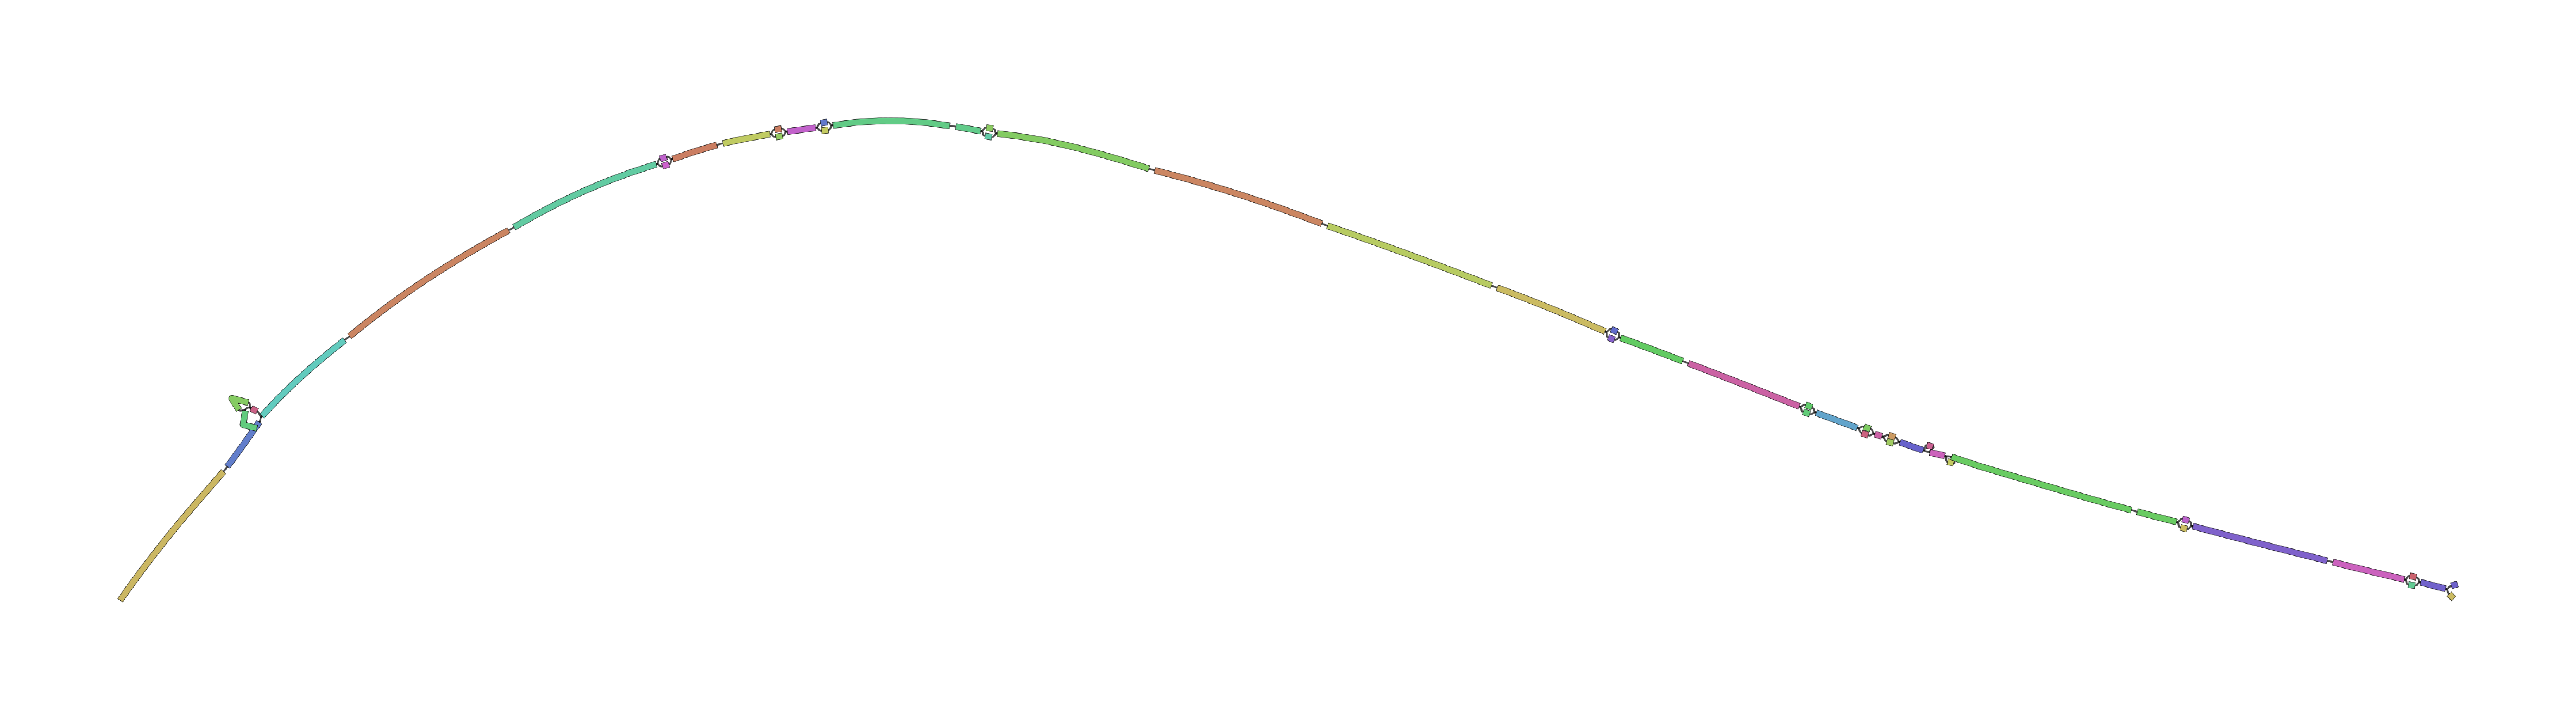
\includegraphics[width=1.0\textwidth]{Chapter2/Figs/vg_view_H-3136_Bandage.pdf}
\caption[Force-directed layout with Bandage]{The graph from figure \ref{fig:vg_view_neato} rendered using {\tt Bandage}.}
\label{fig:vg_view_bandage}
\end{figure}

\subsection{Linear time visualization}

Graph layout algorithms are computationally complex due to their need to iteratively relate all components of the graph to all others.
In these layouts, we can observe large scale features about the topology and organization of the graph.
These views are helpful in many contexts, but the computational complexity of obtaining them should not prevent us from quickly visualizing graphs as we can with linear sequences.
Furthermore, they do not scale efficiently to large path sets, and it is often difficult to understand alignments or other path-related on the graph using them.
Standard graph visualization algorithms exist outside of {\tt vg} as external tools.

To resolve these issues I developed a linear time rendering algorithm that projects a given VG, as indexed by XG, into a vector graphics format using the widely-available graphics library {\tt libcairo}.
The key idea is to use the sequence basis vector $S_\textbf{iv}$ as a coordinate system to position all elements of the graph.
The graph topology itself is laid out in accordance with the node representation in $S_\textbf{iv}$, flowing from left to right at the top of the rendering.
Node lengths are shown using a black bar, with the sequence labels given below.
The graph topology is rendered above the node set, and layout of these edges can be completed in linear time as they are rendered as simple splines connecting node ends.
Paths, or other annotations such as coverage per read set, are displayed below as colored bars matching the subset of the node space that they cover.
Where paths traverse a given node multiple times, an annotation is added to indicate the copy number.
This technique is implemented as {\tt vg viz}, and an example rendering is given in figure \ref{fig:vg_viz}.

\begin{figure}[htbp!] 
\centering    
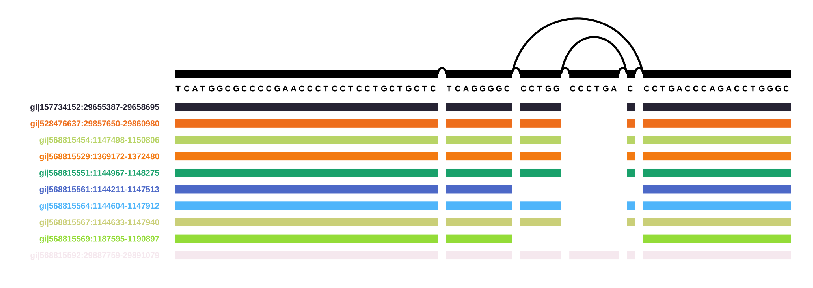
\includegraphics[width=1.0\textwidth]{Chapter2/Figs/vg_viz_H-3136.pdf}
\caption[Linearized variation graph visualization]{The same variation graph in figure \ref{fig:vg_view_dot} rendered using {\tt vg viz}.}
\label{fig:vg_viz}
\end{figure}

It is important to recognize that this approach is lossy.
Path ordering is not clearly represented, as the paths are treated like masks over the sequence space of the graph.
Furthermore, it can be difficult to interpret complex graphs as the topology of the graph is obscured in the simplistic rendering.
{\tt vg viz}'s linear layout treats the graph sequences as a basis space in which other paths or alignments may be interpreted.
This simplistic view is central to many potential applications of {\tt vg}, which I further discuss in section \ref{sec:basis_space}.
The linear scaling of the algorithm should allow it to be applied to whole genomes, provided suitable front-end visualization software can be built, such as in a web interface.

\section{Graph mutating algorithms}

Traversing the topology of the graph and querying its sequence space are important operations when using variation graphs as reference systems.
But to build these graphs, we need to be able to modify them.
Algorithms in graph theory are frequently based on graph transformations, and I have discussed some of them in the context of assembly and whole genome alignment.
{\tt vg} implements many algorithms that alter the graph, but a number are of importance to its development as a system for resequencing, and I detail them here.

\subsection{Edit}

As discussed in section \ref{sec:extending}, the extension of a variation graph to include new sequences and paths can be thought of as a transformation yielding a bijection between the new and old graphs $edit(G, A) \to (G', \Phi)$.
The particular implementation of this editing process is worth considering, as the variation graph data model has a number of particular features which add complexity to editing.
The main issue is that nodes represent more than a single character.

If nodes did represent a single character, then nodes are basically atomic through graph extension.
This approach is that used by POA.
It is simple to edit a ``basepair'' graph of this type: $G = (N, E, P) : |N| = \sum_{\forall n \in N} |seq(n)|$.
We walk through the alignments to it $A = a_1\ldots a_{|A|}$, adding novel bases represented by the alignment ($seq(A) \notin G = N_A$) as new nodes.
Then for each alignment $a_i$, we add edges connecting all of the nodes by edges in the order they would be traversed by the path of the alignment embedded in the graph $p_{a_i} \in G'$, yielding $E_A$.
Finally, we add paths representing the embedded alignments $P_A$.
The resulting graph unifies these additions $G' = (N \cup N_A, E \cup E_A, P \cup P_A)$.

To achieve lower representation costs in graphs with sparse variation, we compress the graph so that nodes may have $seq(n_i) > 1$ and thus we must consider the editing process hierarchically.
We first modify graph $G$ so that every novel sequence will be added at the start or end of a node.
We do this by breaking nodes into multiple derivative nodes when they overlap mappings that do not match the graph using $break(G, A) \to (G', \Phi)$.
For instance, if $seq(n_i) = {\tt GATTACA}$ and we have a SNP ${\tt T} \to {\tt C}$ at offset 4, we would obtain $n_i \to n_i', n_i'', n_i''' : seq(n_i') = {\tt GAT} \land seq(n_i'') = {\tt T} \land seq(n_i'') = {\tt ACA}$.
We can then apply $translate(A, \Phi) \to A'$, and add edges to $G'$ implied by the alignments as we would when editing a graph with single character nodes.

\subsection{Pruning}
%*2.5p 3h*

The number of paths in a sequence graph grows exponentially with the number of variable sites.
As I have discussed, this causes problems for alignment algorithms and graph sequence indexing.
While we can use efficient disk-backed index construction algorithms like GCSA2 to mitigate the effects of this exponential scaling, only a handful of dense clusters of variation in the graph can increase the memory requirements of path enumeration beyond any reasonable level.
Thus there is no reasonable choice but to restructure the graph to limit recombinations in the global sequence index.

We have explored two main techniques for the reduction of graph complexity.
In the first, we prune regions of the graph which have high path complexity using a depth-first search (DFS).
We can optionally add back known haplotypes, in order to mitigate the loss of information from the index.
For VCF-based VGs, where we have haplotype panels, the performance of local alignment is unaffected by the topological complexity, so we only need to apply this pruning to the graph input to GCSA2 indexing.
In assembly graphs, we find that some nodes which represent repeats can have extremely high degree, which causes problems both for indexing and local alignment to the graph.
There, we must remove these nodes in order to use the graph at all.

\subsubsection{$k$-mer ${\cal x}$-edge crossing complexity reduction}

In $k$-mer complexity reduction, we enumerate the $k$-mers of the graph, removing edges when a given $k$-mer crossing them would cross $\geq {\cal x}$ edges.
This can be done by creating a subgraph through a destructive complexity reduction filter, $prune(G, k, {\cal x}) \to G_\textbf{simple}$
We use the same $k$-mer enumeration algorithm that generates a DBG from the variation graph.
For each offest in each node $n_i$ and $\overline{n_i}$, we run a DFS forward until we have read $k$ characters of the graph.
During the pruning operation, instead of emitting the $k$-mers with their contexts, we stop the DFS when we have crossed ${\cal x}$ edges.
We record the edge in $E_\textbf{complex} = \{ e_{ij} : \exists p \in G |p| > {\cal x} \land node(p_{|p|-1} = i \land node(p_{|p|}) = j \}$.
We thus derive the subgraph from the current graph by removing the complexity-inducing edges: $(N, E \setminus E_\textbf{complex}, P) \to G_\textbf{simple}$.
It can be helpful to remove any short subgraphs that result from this pruning, which can be done with a linear subgraph enumeration algorithm and the measurement of the sequence length of each.
A subgraph $G_\textbf{sub} \in G_\textbf{simple} : \forall_{e_{ij} \in N_\textbf{sub}} n_i \in N_\textbf{sub} \land n_j \in N_\textbf{sub}$ must have length $\sum_{\forall n \in N_\textbf{sub}} |seq(n)| \geq {\cal J}$.
By default we use $k=24$, ${\cal x}=3$, and ${\cal J}=33$.

\subsubsection{Filling gaps with haplotypes}

Although removing complex regions will reduce the number of recombinant haplotypes represented by the graph, but it will also remove known haplotypes.
We can retain the complexity reduction without losing sequences in known haplotypes by replacing the pruned regions in $G_\textbf{simple}$ with unfolded copies of each haplotype sequence.
When we have a single reference path, we can accomplish this by overlaying $G_\textbf{simple}$ and $G_\textbf{ref}$.
However, this will not achieve the desired result with even two overlapping paths, as where these differ they would reintroduce the re-combinatorial explosion that we hope to resolve with pruning.
An alternative is to copy the haplotypes in the GBWT index that stretch from one border to the other of each removed region into the removed subgraphs in $G_\textbf{simple}$.
Doing so, we must preserve a mapping between the new nodes and the previous underlying ones in $G$.
This allows matches to the haplotypes to be converted into matches in the base graph.
The exact method by which this filling implemented is described in \cite{siren2018haplotype}.

\subsubsection{High degree filter}

As they separate dense variation into heterozygous bubbles, assembly graphs may feature greater ``smoothness'' than VCF-based graphs locally.
But, in the context of repeats, they can contain nodes with exceptionally high degree.
These highly-connected regions introduce degeneracy in the path space of the graph, and cause problems for $k$-mer enumeration and GCSA2 indexing.
Furthermore, the local alignment methods in VG do not directly support alignment through such dense regions.
This filter is relatively simple, in that we remove nodes with more than ${\cal D}$ edges linking them to the graph, yielding $G_\textbf{prune} : {\cal D} > |\{ e_{ij} \cup e_{ji} \cup e_{\overline{i}j} \cup e_{j\overline{i}} \} \forall i,j \in N_\textbf{prune}|$.

It is not necessary that our local alignment suffers from high-degree nodes.
The problem is that GSSW is provided an alignable graph that is an extracted subset of the full graph.
If this subgraph is extracted using context expansion in the graph, then high-degree nodes will generate extremely large subgraphs.
One solution would be to use the bit-parallel string to graph alignment approach in \cite{rautiainen2018bit}, as this achieves optimal bounds an the size of transformed graph to which we align.
Alternatively, the graph exploration should be more directly linked to the alignment process.
The X-drop aligner {\tt dozeu} could easily be adapted to this approach, as the X-drop parameter would provide a natural limit to the graph exploration.
Such approaches may allow us to tolerate a larger ${\cal D}$, but it seems unlikely that they will allow alignment to be driven through the most-tangled areas of the graph without a large performance penalty relative to graphs with lower maximum degree.

\subsection{Graph sorting}
%*1p 1h*

Order and orient the nodes in the graph using a topological sort.
The sort is guaranteed to be machine-independent given the initial graph's node and edge ordering.
The algorithm is well-defined on non-DAG graphs, but the order is necessarily not a topological order.
To do this we use a bidirected adaptation of Kahn's topological sort \cite{kahn1962topological}, which is extended to handle graph components with no heads or tails.
This algorithm can be understood as a kind of seeded depth first search through the graph.
Where the graph has nodes which are pure heads, it begins there
Otherwise, a set of seed nodes which are stably selected given a particular graph are used to begin the sort.
The details of this procedure are provided in algorithm \ref{alg:pseudotoposort}.

If the reference graph has been sorted, then we can use the given order to generate node identifiers.
These then allow us to efficiently sort subsets of the graph during read mapping.
The extracted subgraph may be sorted by id, and if $\exists e_{ij} : id(n_i) > id(n_j)$ then we know a cycle must exist.
The graph can then be passed to the DAGification procedure.
This allows us to avoid expensive sort operations during read alignment.

Similarly, the sort allows us to project data in the context of the graph into a single dimension.
Provided the graph is manifoldly partially ordered, this projection preserves local structures, which is a desirable property.
This makes the sort applicable to visualization techniques as in figure \ref{fig:vg_viz}.

\begin{algorithm}
  \caption[Pseudo-topological sort]{Pseudo-topological sort}
  \label{alg:pseudotoposort}
  \begin{algorithmic}
    \State $G = (N, E, P)$
    \Comment{A copy of our input graph which we will destructively modify}
    \State $L \gets [ \ldots ]$
    \Comment{Stores the pseudo-topological order}
    \State $S \gets \emptyset$
    \Comment{Set of nodes which have been oriented but not yet traversed}
    \State $V \gets \{ n_i \} \in N : \not \exists e_{ji} \forall n_j \in N$
    \Comment{We start from the head nodes of the graph}
    \If{$V = \emptyset$}
    \Comment{If there are no head nodes, we use ``seed'' nodes}
    \State $V \gets \text{Stably-selected seed nodes} \in N$
    \EndIf
    \While{$V \neq \emptyset$}
      \State $n \gets n \in V$
      \Comment{Select a seed node}
      \State $V \gets V \setminus \{n\}$
      \Comment{Remove it from the input node set $V$}
      \State $S \gets S \cup \{n\}$
      \Comment{Store it in our working set $S$}
      \While{$S \neq \emptyset$}
        \State $n_i \gets n_i \in S$
        \Comment{Remove an oriented node from $S$}
        \State $S \gets S \setminus \{n_i\}$
        \State $L \gets [L[1] \ldots L[|L|], n_i]$
        \Comment{Append it to our output order $L$}
        \For{$\forall n_j : e_{ij} \in E$}
          \State $E \gets E \setminus \{e_{ij}\}$
          \Comment{Remove the edge from our edge set}
          \If{$\not \exists e_{kj} \forall k \in N$}
          \Comment{$n_j$ has no other edges to that side}
          \If{$e_{i\overline{j}}$}
            \State $n_j \gets \overline{n_j}$
            \Comment{Orient $n_j$ so the side the edge comes to is first}
          \EndIf
          \State $N \gets N \setminus \{ n_j \}$
          \Comment{Remove $n_j$ from $N$}
          \State $S \gets S \cup \{ n_j \}$
          \Comment{Insert $n_j$ into $S$}
          \Else
          \Comment{This helps start at natural entry points to cycles}
            \State $V \gets V \cup \{ n_j \}$
            \Comment{Record $n_j$ as a place to start when $S$ is empty}
          \EndIf
        \EndFor
      \EndWhile
    \EndWhile \\
  \Return{$L$} \Comment{Return our pseudo-topologically sorted order and orientation}
\end{algorithmic}
\end{algorithm}
 

\subsection{Graph simplification}

Assembly algorithms often employ a \emph{bubble popping} phase, in which small bubbles, which are graph components connected to the rest of the graph through a single source and sink node, are replaced by linear components representing the most-likely path through the bubble given the read data.
In {\tt vg} we implement a similar technique based on the bubble decomposition of the graph.
Unlike assembly graph bubble popping, we must retain information about the embedded paths and annotations in the variation graph.
Simplification has a number of potential applications, for instance in reducing the complexity of visualizations of large variation graphs.

\section{Graphs as basis spaces for sequence data}
\label{sec:basis_space}

A reference genome allows us to interpret new sequences.
We can consider coverage over the reference genome, but this is incomplete because new sequences may contain variation that we have not seen.
Furthermore, the genome of the new sample may be diploid or polyploid, meaning the genomic state of the sample at a given locus is not trivially expressed as a single sequence.
This leads to the need for variant calling against linear reference genomes.

These steps do not change when our reference is a variation graph, but the scope in which they are relevant may be adjusted to meet our analysis needs.
If we can construct a graph which embeds all of the sequences of all genomes which we are interested in, then all sequences in our study are represented in the sequence space of the graph.
This resolves the separation between reference sequence and variation that is present in standard resequencing.
It also suggests that the intermediate steps in resequencing may be made redundant.
If variation is already available during alignment then there is no need for a variant detection phase.

However, if the graph does not include variation in our samples, then variant calling is required.
In {\tt vg} we have implemented several methods to do so.
Similarly, we have implemented coverage transformations of read sets that may be used directly in downstream analyses.

\subsection{Coverage maps}

Numerous population genetic analyses are based on matrix transformations of a collection of genomes.
Such models can be used to infer population structure and phylogeny, as well as to associate phenotypes to features in the genome such as causative variants.
If the variation graph used as a reference contains all sequences relevant to our anaylsis, then a matrix of per-base coverage of the graph by sample will provide nearly-full information to downstream analyses.
We cannot observe structural variation that does not result in coverage changes, such as balanced events like inversions.
Also, some local patterns of variation between successive small variation will not be differentiable.
If we were to annotate edge coverages, this method would produce a result equivalent in information content to a markov model.
It is thus clear that any coverage based index will be lossy relative to the full read set.
However, the lossiness reduces the information cost of storing and processing these coverage maps.
As I described in section \ref{sec:coverage_index}, in {\tt vg} I developed an efficent method to accumulate coverage information of this kind across the graph, but I have limited experimental results describing its utility.

\subsection{Bubbles}

In a sequence graph, a \emph{bubble} is a pair of paths which start and end at the same nodes ($s$, $t$) but are otherwise disjoint in the graph \cite{zerbino2008velvet}.
Bubbles encompass our intuition about genetic variation in graphs.
A homologous sequence corresponding to the common start and end nodes in the bubble flanks two or more alternative alleles in the middle.
These structures were first considered only in the process of finding small variation, and it was only in recent years that methods were developed to efficiently enumerate all bubbles of any size in DAGs \cite{birmele2012efficient}.

Bubbles can nest and contain more complicated internal structures between the paths through them.
The bubble may be generalized to the idea of a \emph{superbubble}, which is a directed, acyclic component of a graph with a single head and tail node \cite{onodera2013detecting}.
As for bubbles, efficient enumeration of superbubbles is possible in a DAG \cite{brankovic2016linear}.
The optimal method relies on a recursive topological sort of the graph to structure the nested bubbles.
Candidate node starts ($s$) and ends ($t$) are found following the definition of a superbubble.
The set of candidates is then validated by range min queries (RMQ) to produce the set of superbubbles.
As sort is linear $O(|N| + |E|)$, and the candidate enumeration and RMQ may be implemented on the sorted graph in $O(1)$ each, this yields a linear time algorithm for the enumeration of superbubbles.

The DAG requirement of this method is a significant limitation as it prevents us from directly applying the bubble finding to an arbitrary graph.
In order to apply the superbubble enumeration to a graph we must first DAGify it.
In response, along with Benedict Paten and others, I worked to further generalize the idea of a genetic site to work on arbitrary bidirectional sequence graphs \cite{paten2018superbubbles}.
To formulate a generalization of superbubbles, we introduce the concept of a \emph{snarl}, which is any graph component connected to the rest of the graph by less than two bordering nodes\footnote{In the paper the formulation is based on a biedged graph akin to the Enredo graph, but as we note a node-based formulation is equivalent and matches the other models in this section.}.
Snarls whose internal separated component are acyclic and do not contain any tips are \emph{ultrabubbles}.

Paten observed that trees embedded in the Cactus graph transformation of a variation graph corresponded to the standard concept of superbubbles.
Specifically, the cactus graph is transformed into a \emph{cactus tree} in which each simple cycle in the cactus graph becomes a special kind of node.
Various rootings of this tree may then be used to define a hierarchy of bubbles.
The bidirectional nature of the variation graph mean that snarls can embed each other in a manner akin to how the twist used to generate a M\"{o}bius strip results in it having a single surface and border.
In these cases the resulting cactus tree will support multiple ultrabubble tree rootings, and so unlike the bubble and superbubble decompositions for DAGs the ultrabubble decomposition is not complete.
We can enumerate a subset of these by identifying bridge edges (typically representing tips) in the ``bridge forest'', which is the result of a contraction of the cycles in the cactus graph into a set of top-level cycle representing nodes, and then use them to produce various rootings of the cactus tree.

Ultrabubbles and superbubbles provide a complete framework in which to reason about the hierarchy of variable genetic sites embedded in a graph.
As such they provide the basis for generic models of genotype inference based on variation graphs which are capable of genotyping any kind of genetic variation, including structural variation as well as nested variation in the same model as SNPs and indels.

\subsection{Variant calling}

Given a definition of variable genetic loci in the graph, we can build a genotyping system capable of generating genotype calls in the context of the graph.
In {\tt vg} we have explored two such methods.
The first, originally implemented in {\tt vg call}, generalizes the concepts first implemented in {\tt samtools mpileup} to work on the graph.
A set of alignments are first reduced to pointwise edits against the graph and per base coverage of the graph.
This graph ``pileup'' is then processed by a genotyping algorithm that considers genetic sites using the ultrabubble model.
A schematic overview of the method is shown in figure \ref{fig:vg_call}.

\begin{figure}[htbp!]
  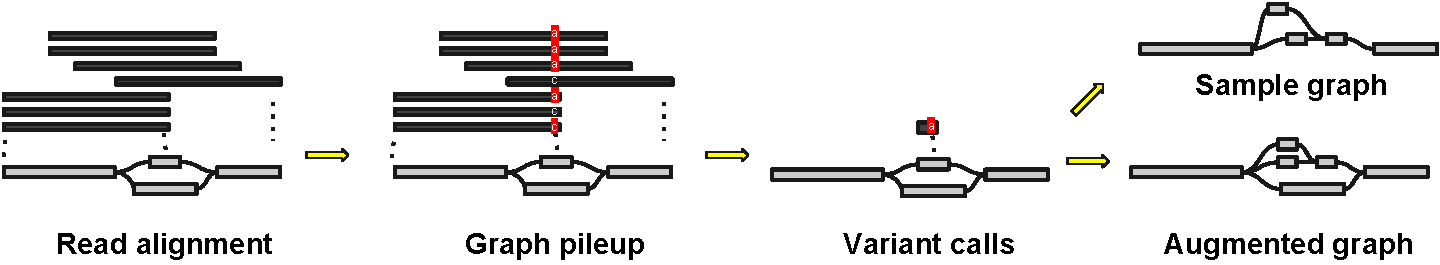
\includegraphics[width=1.0\textwidth]{Chapter2/Figs/vg_call.pdf}
  \caption{
    Pileup variant calling with {\tt vg call}
    }
  \label{fig:vg_call}
\end{figure}

The second model, implemented in {\tt vg genotype}, embeds the alignments in the variation graph using $edit(A, G_\textbf{base}) \to (G_\textbf{aug}, \Phi_{\textbf{aug}\to\textbf{base}})$, and then genotypes across the ultrabubbles of $G_\textbf{aug}$ which are supported by reference paths in $G_\textbf{base}$ or reads.
As the resulting genotypes are represented as unordered sets of paths in $G_\textbf{aug}$, they are projected back into the coordinate space of $G_\textbf{base}$ using the translation $\Phi_{\textbf{aug}\to\textbf{base}}$.
An overview of the process is shown in figure \ref{fig:vg_genotype}.

\begin{figure}[htbp!]
  \centering
  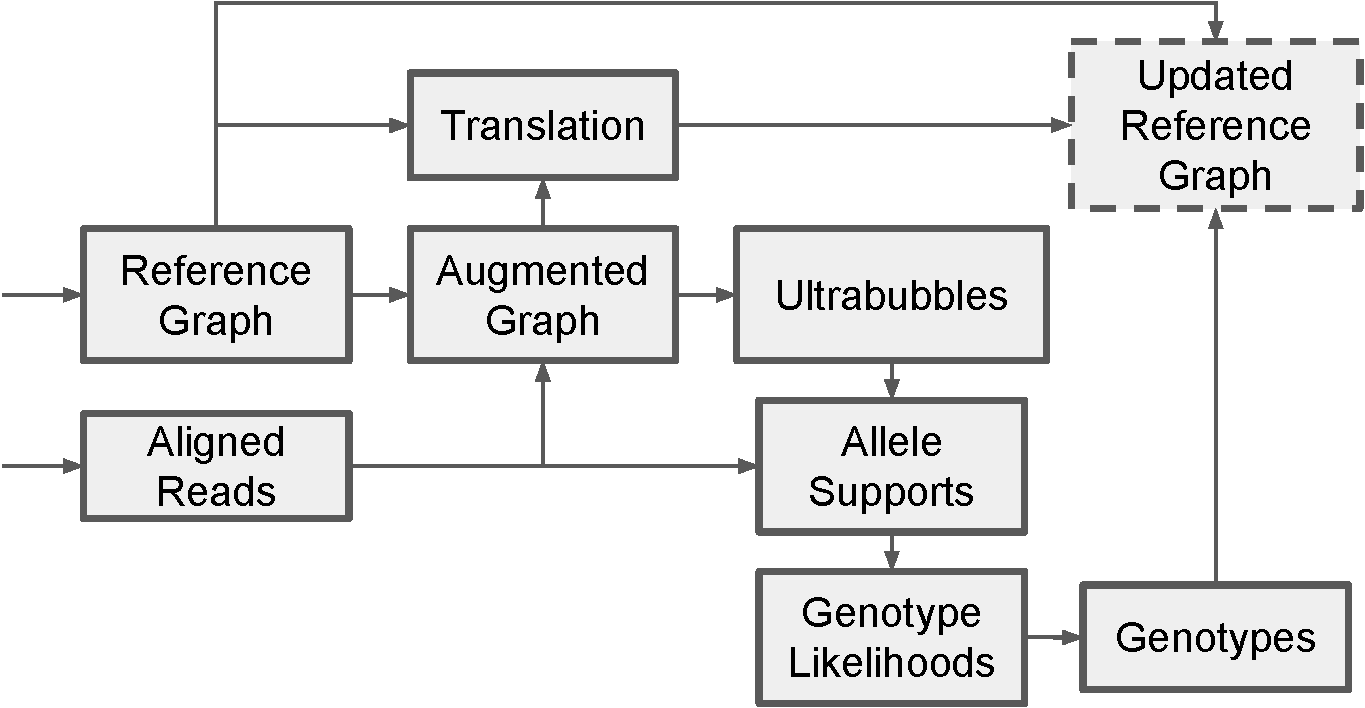
\includegraphics[width=0.7\textwidth]{Chapter2/Figs/vg_genotype.pdf}
  \caption{
    Graph augmentation-based variant calling in {\tt vg genotype}
    }
  \label{fig:vg_genotype}.
\end{figure}

While principled, the full augmentation model in {\tt vg genotype} is very expensive to compute.
The pileup model has proven to be more efficient.
Over time {\tt vg call} has been adjusted to implement a variant of the full graph augmentation model in {\tt vg genotype} where the graph is augmented only with sequences supported by some number of alignments at a given quality threshold.
Both methods employ a diploid specification of the genotyping model in freebayes \cite{garrison2012haplotype} to develop their posterior estimates of variant quality.
The generalization of SNP and indel calling to haplotype calling implemented in freebayes corresponds to the same allele model used in both {\tt vg} variant calling methods.
In all alleles correspond to DNA sequences of arbitrary length, anchored at the ends to the reference genome (in the case of freebayes) or to the rest of the graph (as in the ultrabubbles used in {\tt vg}).

The complexity of running genotyping in the graph has slowed development of these methods.
Currently they are outperformed by standard variant calling methods based on the linear reference, as indicated by our results in the PrecisionFDA variant calling challenge that I will describe in the next chapter.

%\subsection{MEM matching to the bidirectional GBWT}

%\section{Contributions to related computational methods}

% in this chapter I've described things that I've done
% as a consequence of being in this work, here are things that I helped other people to build
% list papers, give references

% gpBWT
% GCSA2
% ...

%!TEX root = ../thesis.tex
%*******************************************************************************
%****************************** Second Chapter *********************************
%*******************************************************************************

\chapter{Variation graphs}

\DIFaddbegin \label{chapter:variation_graphs}

\DIFaddend \ifpdf
    \graphicspath{{Chapter2/Figs/Raster/}{Chapter2/Figs/PDF/}{Chapter2/Figs/}}
\else
    \graphicspath{{Chapter2/Figs/Vector/}{Chapter2/Figs/}}
\fi

\emph{Variation graphs} (VGs)\footnote{I will refer to variation graph as VG, and to the software implementation of the VG model {\tt vg}}, previously introduced in section \ref{sec:the_variation_graph}, combine a bidirectional sequence graphs with paths that model sequences as walks through the positional space of the graph.
They link graphical models and linear sequence models.
This allows them to be used to model the relationships between collection of sequences, including all variation contained therein.
The encapsulation of these two divergent ways of modeling about bioinformatic data systems allows them to bridge traditionally isolated analysis modalities.

In this chapter, I will articulate the variation graph model and lay out the algorithms and data structures that enable its use as a reference system in pangenomic resequencing.
First I will provide formulations for the graph, its paths, edits, alignments, and genotypes define within it.
Then I will present algorithms that induce the variation graph from different data models introduced in the previous chapter.
I describe the serialization techniques used to exchange variation data via computer files or network connections.
I develop index structures to enable queries of the graph's topology, sequence, and path spaces, and algorithms to derive optimal alignments to the graph.
Understanding variation graphs requires techniques to visualize them, and I will present various approaches, each with particular advantages and drawbacks.
Working with variation graph references necessitates a number of graph-modifying operations, including augmentation, sorting, pruning, and bubble simplification.
Finally, I will discuss how variation graphs can provide normalized basis spaces for the analysis of pangenomes, such as through various projections of alignment sets and the graph including coverage maps, ultrabubble decomposition, and haplotype matching.

\DIFaddbegin \begin{figure}[htbp!]
  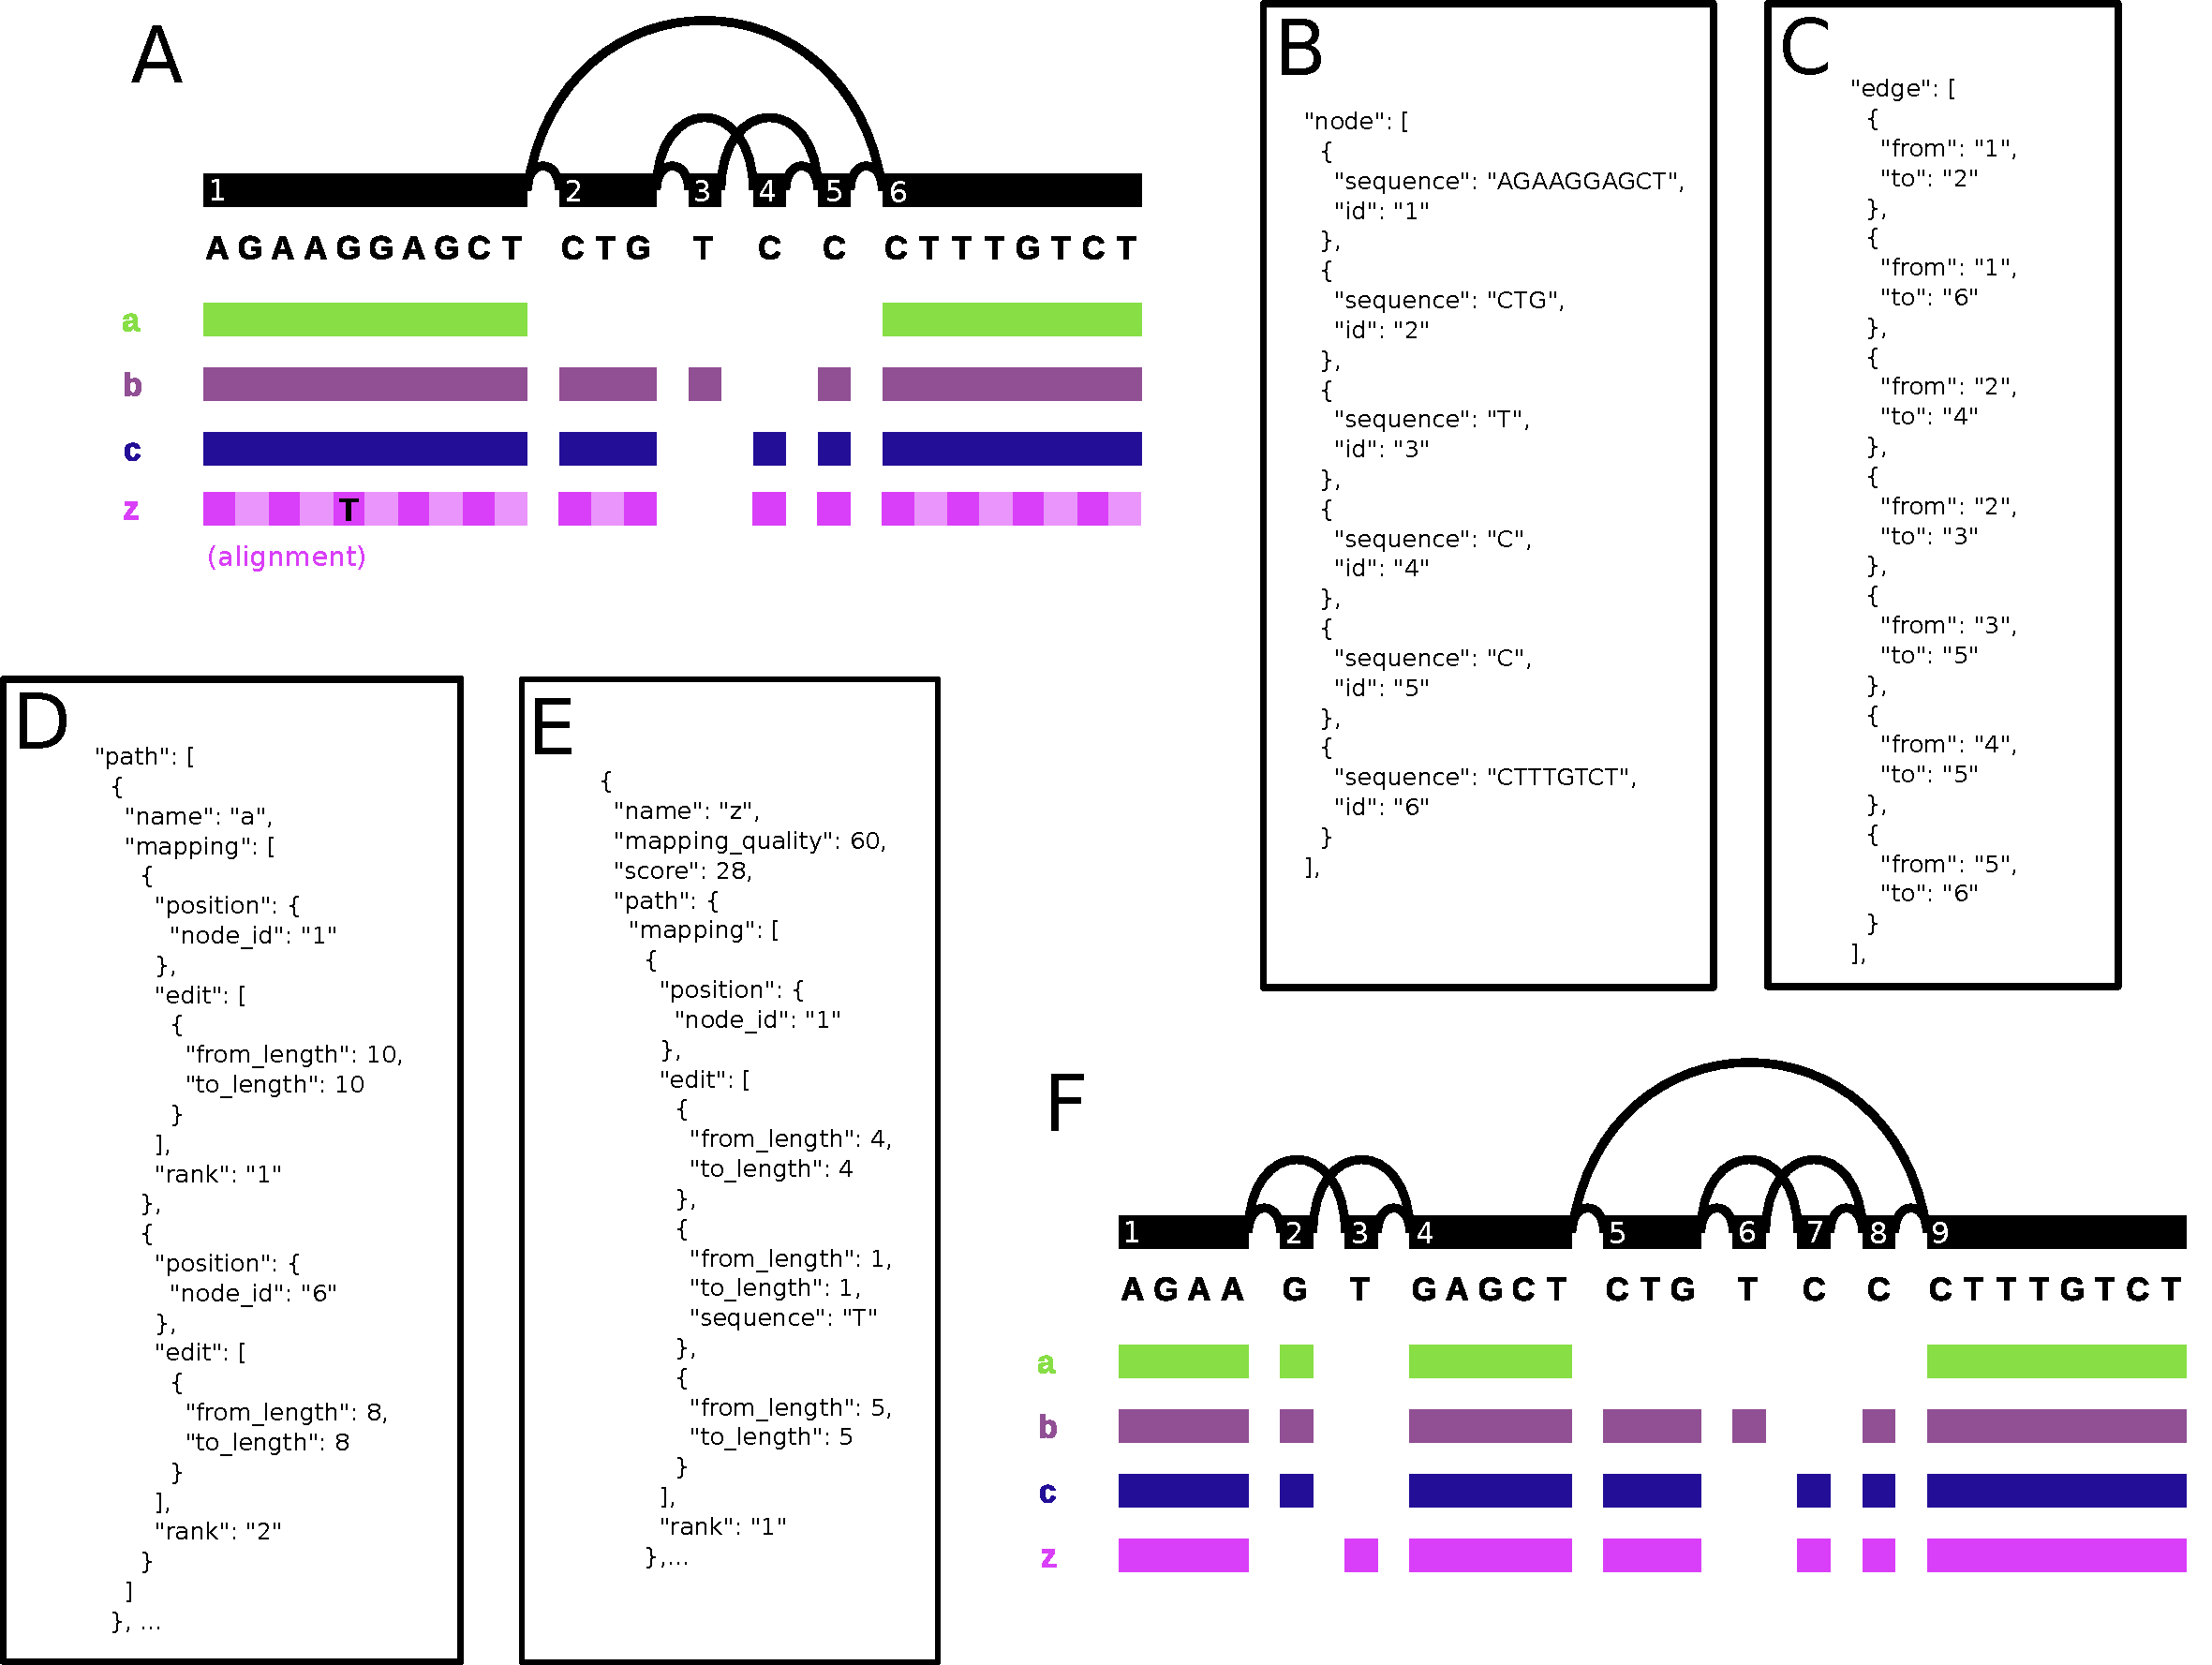
\includegraphics[width=\textwidth]{Chapter2/Figs/example_vg_construction.pdf}
  \caption[The basic elements of a variation graph]{
    \DIFaddFL{A step in the progressive construction of a variation graph from homologous fragments of four haplotypes in the GRCh38 alternate allele set for the HLA gene DQB1-3119.
    (A) shows variation graph constructed by progressive alignment of three sequences labeled }\emph{\DIFaddFL{a}}\DIFaddFL{, }\emph{\DIFaddFL{b}}\DIFaddFL{, and }\emph{\DIFaddFL{c}}\DIFaddFL{.
    The graph topology is shown in at the top of the panel, with nodes represented by black bars, labeled by their node IDs (white numbers), and with edge connections between nodes shown by arcs above.
    Paths are indicated in the colored bars below, with a identifying name to the left.
    This graph is partially ordered, without cycles, and so the sequences of paths may be enumerated by concatenating the node sequences above the filled portions of each of the path rows.
    A fourth sequence }\emph{\DIFaddFL{z}} \DIFaddFL{has been aligned to the graph, and is shown in a checkerboard magenta pattern.
    It contains a single SNP relative to the graph, which is shown by the black }{\tt \DIFaddFL{T}} \DIFaddFL{matching the fifth position of the first node.
    The JSON presented in (B) describes the full node set of the graph in (A), while (C) lists the edges.
    (D) shows the path }\emph{\DIFaddFL{a}} \DIFaddFL{embedded in the graph in full. Other paths are not provided, but their overall format is the same.
    (E) describes the alignment of }\emph{\DIFaddFL{z}} \DIFaddFL{against graph (A). Only the beginning of the path of }\emph{\DIFaddFL{z}} \DIFaddFL{against (A) is given.
    The first mapping in the path describes a SNP between the matching subsequence in }\emph{\DIFaddFL{z}} \DIFaddFL{and $n_1$.
    Note the second edit in the mapping, which specifically describes the SNP as a replacement of a subsequence in $n_1$ by }{\tt \DIFaddFL{T}}\DIFaddFL{.
    Graph (F) is the result of the application of the $edit$ operation to graph (A) and alignment }\emph{\DIFaddFL{z}}\DIFaddFL{.
    The node IDs have been reassigned.
    The inclusion of the SNP increases the node count of the graph by 3.
    Path $[n_1]$ in graph (A) maps to $[n_1,n_2,n_4]$ in (F).
  }}
  \label{fig:vg_illustrative_example}
\end{figure}

\DIFaddend %\section{An extensible graphical model of many sequences}
\section{A generic graph embedding for genomics}

We define a \emph{variation graph} to be a graph with embedded paths $G = (N, E, P)$ comprising a set of \emph{nodes} $N = n_1 \ldots n_M$, a set of \emph{edges} $E = e_1 \ldots e_L$, and a set of \emph{paths} $P = p_1 \ldots p_Q$, each of which describes the embedding of a sequence into the graph.
By generalizing these paths to support edits against the graph, we provide a mechanism to describe relations between the graph and other sequences.
Augmenting the path with additional information important to sequence analysis allows us to construct an \emph{alignment}.
Collections of pairs of paths covering the space of two graphs describe a graph to graph alignment, or \emph{translation} which can be generated when the graph is edited, to allow for the projection of coordinates and sequences in one graph into the space of the other.
A limited form of this translation is a \emph{genotype}, which maps the implied bubble formed across multiple copies of a homologous locus into the space of the graph.
Collections of genotypes are the primary output of resequencing.
Phasing algorithms extend genotypes into longer phased haplotypes, which we record as paths through the graph.
These data models thus provide a sufficient informational basis for resequencing against variation graphs.

\subsection{The bidirectional sequence graph}

Each node $n_i$ represents a sequence $seq(n_i)$ that is built from an alphabet $\Sigma = \{ {\tt A, C, G, T, N} \}$. Nodes may be traversed in either the forward or reverse direction, with the sequence being reverse-complemented in the reverse direction.
We write $\overline{n_i}$ for the reverse-complement of node $n_i$, so that $seq(n_i) = revcomp(seq(\overline{n_i}))$.
Note that $n_i = \overline{\overline{n}}$. For convenience, we refer to both $n_i$ and $\overline{n_i}$ as ``nodes''.

Edges represent adjacencies between the sequences of the nodes they connect.
Thus, the graph implicitly encodes longer sequences as the concatenation of node sequences along walks through the graph.
Edges can be identified with the ordered pairs of oriented nodes that they link, so we can write $e_{ij} = (n_i,n_j)$.
Edges also can be traversed in either the forward or the reverse direction, with the reverse traversal defined as $\overline{e_{ij}} = (\overline{n_j},\overline{n_i})$.
VGs can contain ordinary cycles (in which $n_i$ is reachable from $n_i$), reversing cycles (in which $n_i$ is reachable from $\overline{n_i}$), and non-cyclic instances of reversal (in which both $n_i$ and $\overline{n_i}$ are reachable from $n_j$).

\DIFdelbegin \subsection{\DIFdel{Paths with edits}}
%DIFAUXCMD
\addtocounter{subsection}{-1}%DIFAUXCMD
\DIFdelend \DIFaddbegin \DIFadd{The bidirectional sequence graph underlying the variation graph model is illustrated in panels A, B, and C of figure \ref{fig:vg_illustrative_example}.
}\DIFaddend 

\DIFaddbegin \subsection{\DIFadd{Paths with edits}}
%DIF >  TODO fixme this needs an explanation of what's different between paths in the graph and those in alignments
\DIFaddend We implement paths as an edit string with respect to the concatenation of node subsequences along a directed walk through the graph.
We do not require the alignment described by the edit string to start at the beginning of the sequence of the initial node, nor to terminate at the end of the sequence of the terminal node.
To allow the path model to support differences from the graph, each path is composed of a series of node mappings $p_i = m_1 \ldots m_{|p_i|}$ which are semantically identical to the alignment format used by standard aligners.
Each mapping $m_i = ( b_i, \Delta_i )$ has a starting position encoded as a node and offset in the graph $b_i = ( n_j, o_i )$ and a series of edits $\Delta_i = \delta_1 \ldots \delta_{|m_i|}$.
Edits $\delta_i = ( f_i, t_i, r_i )$ represent a length $f_i$ in the graph node $n_j$ (a ``from length'' in the reference), a length $t_i$ in the sequence the path encodes (a ``to length'' in the query), and an additional sequence $r_i$ that would replace the sequence at the given position in the reference in order to transform it into the query.
In the case of exact matches, we allow the replacement sequence $r_i$ to be empty.

Alignments are often described in terms of matches, mismatches, and indels.
We encode matches when $f_i = t_i \land r_i = \emptyset$, single mismatches when $f_i = t_i = 1 \land r_i \neq \emptyset$, deletions when $f_i > 0 \land t_i = 0 \land r_i = \emptyset$, and insertions when $f_i = 0 \land t_i > 0 \land r_i \neq \emptyset$.
As paths are described by a series of mappings with independent positions, they can represent all kinds of structural variation relative to the graph.
When mapping positions are always at the start of a node, the edit set for the path contains only matches, and the edges traversed by the path are all present in the graph\footnote{Note that paths may contain disjoint mappings that are not connected by edges in the graph, which allows them to represent structural variations.}, we say that the path is \emph{embedded}.
The paths from which we construct the variation graph are fully embedded, and in practice paths that contain differences occur only in the alignment of new sequences into the graph.

\DIFaddbegin \DIFadd{The example variation graph in figure \ref{fig:vg_illustrative_example} panel A contains several paths, while panel D explicitly describes a portion of one of the paths using an equivalent model to the one described here.
}

\DIFaddend \subsection{Alignments}
\label{sec:alignments}

Auxiliary read information is important when analyzing collections of DNA sequencing data sets.
Each read has a name, and an identity related to a particular sequencing experiment.
It may be related to a particular genomic sample or individual.
DNA sequence reads themselves result from a previous set of analyses run on raw observations derived from DNA, perhaps fluorescence or current traces or images.
The process of collapsing this raw information into the sequence read yields a confidence in addition to a base call.
These are recorded in a quality string in FASTQ.
The need to collect this information has resulted in the development of the SAM/BAM sequence alignment format, which provides a standard for linking the called bases (sequence), quality information, read name, features of the alignment against a reference genome and additional optional typed annotations.

I follow this same model in developing an alignment format for read alignments to the graph.
An aligned set of sequences $Q$, $A = a_1 \ldots a_{|Q|}$, represents a sequencing experiment.
Each aligned read connects a sequence, an (optional) quality string, a path through the graph including possible edits, and an optional set of $D_i$ annotations: $a_i = (s_i, q_i, p_i, k_1\ldots k_{D_i})$.
In principle the read sequence can be reconstructed from the path, but retaining the sequence information makes the alignment object lossless with respect to the input FASTQ and provides redundancy which can help in data processing.

\DIFaddbegin \DIFadd{Panels A and E of figure \ref{fig:vg_illustrative_example} demonstrate how an alignment to a variation graph can encode putative variation, in this particular case encoding a SNP.
}

\DIFaddend \subsection{Translations}
\label{sec:translation}

A generalization of the alignment is the translation set $\Phi = \phi_1 \ldots \phi_{|\Phi|}$, which relates paths in different graphs to describe the mapping between them.
A translation $\phi = (p_f, p_t)$ defines the projection between two paths which may arise in the context of two graphs $G_f$ and $G_t$.
In this use each $p_f$ corresponds to a path relative to $G_f$ (conventionally the base or reference graph), and each $p_t$ to some path in $G_t$.

If each node and edge and path in both graphs is represented in some graph translation in $\Phi$ then it provides an isomorphic relationship between the graphs.
Provided each $\Phi$ encodes an isomorphism, then we can layer a series of $\Phi_i$ together to provide a coherent coordinate space across any number of updates to a given graph.
Consider a function pattern $translate$, which allows the projection of paths relative to $G_f$ through translations $\Phi$ to yield paths in $G_t$: $translate(p_i, \Phi) \to p_j \in G_t$, and similarly allows the transformation of a base graph into a target graph: $translate(G_f, \Phi) \to G_t$.
If we have a series of $(G_i, \Phi_1) \ldots (G_\rho, \Phi_\rho)$, where $translate(G_i, \Phi_i) \to G_{i+1}$ and thus each $\Phi_i$ describes an isomorphism between $G_i$ and $G_{i+1}$, then we can generate a graph translation $\Phi_\Delta$ providing $translate(G_1, \Phi_\Delta) \to G_\rho$.
We build this graph translation with the function $layer(\Phi_\alpha, \Phi_\beta) \to \Phi_{\alpha \circ \beta}$ by rewriting each path translation $\phi_i \in \Phi_\alpha$ so that its $p_t$ refers to $G_\beta$.
We do so by projecting the $p_t$ through $\Phi_\beta$, and finally adding any $\phi_j \in \Phi_\beta$ for which $p_f = \emptyset$, as these represent insertions of new sequence in $G_\beta$ relative to $G_\alpha$.

\subsection{Genotypes}
\label{sec:genotypes}

As path to path relationships can provide descriptions of allelic diversity, they form the basis for a graph-relative genotype encoding.
To represent the exact genotype of a particular sample with ploidy $\nu$ at a given locus $\iota$ we can simply collect the multiset of alleles $\pi_\iota = ( p_1 \ldots p_\nu)$.
We could alternatively build a probabilistic model $\varpi$ of an unphased genotype by using a set of $\mu$ alleles $\{ p_1 \ldots p_\mu\}$.
To do so, we associate likelihoods $\gamma_\xi$ for each possible genotype $\pi_{\iota_\xi}$ that could be sampled from the alleles such that $\varpi = \gamma_1 \ldots \gamma_{\frac{\mu!}{\nu!(\mu-\nu)!} }$.
In practice, we develop our $\gamma_\xi$ out of quality information from the reads and a sampling model related to $\nu$ \cite{garrison2012haplotype,li2011statistical}.
Existing genotyping models can be applied to drive genotyping using read sets aligned to the graph, and the output of the genotyper is defined fully in the space of the graph.

\subsection{Extending the graph}
\label{sec:extending}

Given an alignment $a_i$, we can edit the graph $G$ so that it includes the alignment and the sequence it represents as an embedded path, $augment(G, a_i) \to (G', \Phi)$, such that $translate(p_i, \Phi) \in G'$.
To update the path space of the graph we project all paths, including that of $a_i$, through the translation implied by the augmentation of the graph with $p_i$.
Any other alignment $a_j$ whose path $p_j$ overlaps $p_i$ would no longer be valid, although it could be projected through the graph translation $\Phi$ as well to express it in the space of the new graph $G'$.
Updating the graph one alignment at a time is inefficient as we need to build and layer a new translation for each alignment.
It is simpler to edit the graph in a single step, taking a collection of alignments and including them in the graph, $edit(G, A) \to (G', \Phi)$.

One way to accomplish this is to first take the set of unique mappings represented in the paths of $A$, $\Omega = \{ m_1 \ldots m_{|\Omega|}\}$, and for each $m_i$ cut $n_i$ at the breakpoints where any new variation would need to be added in, adding new nodes to represent the cut portions.
Then, walking through each alignment we add in unique novel sequences and their linkages to the preexisting nodes or new breakpoints to the graph.
This process will disrupt the identifier space of the nodes and edges of the graph, but it naturally yields a translation that can be used as described in section \ref{sec:translation}.
Both alignments and genotypes are based on paths, so this mechanism can be used to extend the graph based on any sequence level differences observed through alignment or variant calling.

\DIFaddbegin \DIFadd{Figure \ref{fig:vg_illustrative_example} provides an example to provide a concrete intuition about the $edit$ function.
Editing the graph in panel A with the alignment of sequence }\emph{\DIFadd{z}} \DIFadd{yields the graph in panel F.
The corresponding translation is described in the figure legend.
}

\DIFaddend \section{Variation graph construction}

We will use variation graphs as the core model for a number of essential processes in genome inference.
This model can represent many graphical sequence models used in genomics.
Each one necessitates conversion into the variation graph model.
Here I describe the transformation of a number of graphical models into variation graphs, including MSAs, assembly graphs, and alignment graphs induced from pairwise alignments.
In some cases the conversion is direct, but in others it requires the addition of new labels to our model.
Variation graphs may also be built from first principles, provided a function that aligns a sequence into the graph and the editing operations described in \ref{sec:extending}.

\subsection{Progressive alignment}

If we have a series of $k$ queries $q_1 \ldots q_k$, then we can build a progressive alignment by a series of edit and alignment operations applied to the variation graph.
First, take the empty graph $G_\emptyset$, to which any alignment will yield a path $p_1$ that has no mappings and which encodes the query sequence $q_1$ as a replacement sequence in the path.
We then edit the graph to add the sequence using $edit(G_\emptyset, p_1) \to G_1$.
For each subsequent $q_j$ we obtain the next graph by finding the alignment $align(q_j, G_j) \to p_j$ and editing the graph with it to yield the next graph $edit(G_j, p_j) \to G_{j+1}$ until $j = k$ and we obtain our final graph.
This simple approach is attractive as it allows the variation graphs to be built from whole sequences using only techniques that are native to the variation graph model itself.
However, it is obviously order dependent, with potentially different results if the set of input sequences are presented in different orders.
I later presents results based on this multiple sequence to graph alignment process, {\tt vg msga}.

\subsection{Using variants in VCF format}
%*1.5p 1h*
As discussed in section \ref{sec:seq_dag_vcf}, the VCF format that is popular in resequencing implies a sequence DAG.
We can consider how to build a trivial variation graph using the core operation $edit$.
First, we build a variation graph from the reference genome $Q_\textbf{ref}$ : $G_\textbf{ref}$.
This graph contains one path $p_\textbf{ref}$ : $seq(p_\textbf{ref}) = Q_\textbf{ref}$.
As described in section \ref{sec:genotypes} each locus reported in VCF can be encoded as a set of paths $P_\textbf{vcf} = p_1 \ldots p_V$, each representing a different allele.
We now edit the graph to embed these allele paths, $edit(G_\textbf{ref}, P_\textbf{vcf}) \to G_\textbf{vcf}$.
It is possible to regenerate the VCF file input by walking the positions of $p_\textbf{ref}$ and enumerating the overlapping paths as alleles in VCF format.

For efficiency, we have not implemented VCF to variation graph conversion with specifically this algorithm, but instead build up $G_\textbf{vcf}$ by walking along the reference genome $Q_\textbf{ref}$ and processing each locus sequentially.
This exploits the partially ordered property of the VCF to limit memory requirements.
For regions before, after, and between variant records at reference offsets $i$ and $j$ we add a node $n_\textbf{curr} : seq(n_\textbf{curr}) = substr(Q_\textbf{ref}, i, j)$, linking these by edges to those nodes ending at position $i$ of the reference and adding corresponding mappings for the reference path to $p_\textbf{ref}$.
At simple variant sites we add each of the alleles as a new node $n_{\textbf{var}_i}$, including an edge for each $e_{\textbf{curr} \prec \textbf{var}_i}$.
Here we also handle the reference allele differently in that we append a mapping $m_\textbf{ref} = ((n_\textbf{ref}, 0), \emptyset)$ to $p_\textbf{ref}$.

As long as the VCF records are ordered, this process allows for streaming conversion of the VCF format into a variation graph.
However, VCFs used to represent structural variation often do not describe a fully-ordered series of loci.
For instance, a large deletion may be described in one record, and followed by a number of records describing variation on the reference within the scope of the deletion.
In the graph, this results in the nesting of bubbles, and requires a deviation from a simple streaming algorithm in order to be handled.
Deletions must be recorded and linked into the downstream portion of the graph as it is later generated.

VCFs may also encode phased haplotypes, which, like the reference, have a natural representation in the graph as paths.
Parsing these may require multiple passes over the VCF due to the memory requirements for storing large numbers of haplotypes uncompressed and cross-indexed to allow traversal in RAM.
To prevent $O(H|G_\textbf{vcf}|)$ growth of the required memory to store these, we implement compression strategies on the haplotype set that exploit their repetitiveness.
The VCF format does not impose a semantic requirement that the encoded haplotypes are valid, which introduces some complexity in the implementation of this method.
We must break haplotypes where they are found to be invalid in order to record them in VG format.
For instance, a phased VCF may report more than $\nu$ (expected ploidy) alleles for a given individual, such as when deletion and SNP variants overlap.
We expect these haplotype paths to be embedded in the graph.
Although haplotype sets are equivalent to large collections of paths, we term their components \emph{threads} to indicate that they have a simpler representation than arbitrary paths.

\subsection{From gene models} % (GFF)
\label{sec:construct_from_gff}

A reference-based RNA splicing graph is usually expressed as a set of named intervals in BED or the General Feature Format (GFF).
As with the generic VCF generation algorithm, we can convert the transcripts to alignments $A$ relative to the graph.
Then we can then embed the transcript paths in the graph $edit(G_\textbf{ref}, A) \to G_\textbf{splice}$.
Any transcript in our set is thus encoded by the graph, and can be matched to it directly with alignment.
The resulting structure will also support novel isoforms built with splices from the known set.

\subsection{From multiple sequence alignments}
%*0.5p 0.5h*
A multiple sequence alignment in matrix form has a simple translation into a sequence DAG and thus a VG \cite{lee2002POA}.
Given a set of sequences $Q = q_1 \ldots q_\kappa$ their $\upsilon$-long mutual alignment may be described in a $\kappa \upsilon$ matrix $X$ designed to maximize $\sum_{i=1}^{\upsilon} \sum_{j=1}^{\kappa} \sum_{k=1}^{\kappa} \delta_{X_{ij}X_{ik}}$, where $\delta$ is the Kronecker delta, or some generalization of this.
The alphabet used to encode the matrix is the same as the input sequences with the addition of a special gap character $\Box$ which does not match itself, and gaps thus do not contribute positively to the matrix score.
To build a variation graph $G_\textbf{msa}$ from the MSA we proceed from $i = 1 \to \upsilon$ through $X$.
For each unique character ${\cal B}$ in the query alphabet $\Sigma \setminus \Box$ found in each row $i$, we create a node $n_{\cal B}$ in $G_\textbf{msa}$ and append a mapping to each path $p_i$ for which $n_{\cal B} \in q_i$.
We construct the edges of $G_\textbf{msa}$ by taking the distinct pairs of consecutive node traversals found in the path set $P_\textbf{msa}$ produced after the generation of the nodes in MSA traversal.
Adding add an edge $e_{ij}$ for each pair of nodes $(n_i, n_j)$ consecutively traversed in $P_\textbf{msa}$ ensures that our sequences are present as walks through the graph.
We can optionally compact series of nodes (which represent single characters) where no furcations occur to obtain a simpler graph.

Instead of a matrix, we can formulate the multiple alignment as an alignment graph (described in section \ref{sec:genome_alignment_graphs}).
By making this graph bidirectional, and thus equivalent in information content with the Enredo graph, it becomes equivalent to a variation graph.
Aligners that produce data formats of this type, such as Cactus \cite{Paten:2011fva}, can thus be used to produce VGs, so long as the relationship between the input sequences and the graph is recorded and can be converted into a path description.
In section \ref{sec:yeast_cactus} I discuss the use of this method to build a pangenomic reference system for a diverse set of yeast strains.

\subsection{From overlap assembly and deBruijn graphs}
%*2p 1.5h*

Overlap-based sequence graphs used in assembly, described in sections \ref{sec:overlap_graphs}, \ref{sec:de_bruijn_graphs}, and \ref{sec:string_graphs}, are nearly identical to variation graphs.
The critical difference between these models and the variation graph is that they attach a label to each edge (or node) describing the alignment between the pair of nodes (or edges) which they connect.
Variation graphs do not support such a feature in their basic definition, as it is unimportant for any use besides temporarily representing overlap graphs.
We call the process of transferring sequence information from the edges to the nodes \emph{bluntification}.

We start by assigning the sequence of each node to be the sequence of the corresponding read.
If we shorten the sequence of a node to reduce an overlap between a pair of nodes, it will render other overlaps on the same nodes incorrect.
Thus, it is essential that the bluntification algorithm work by the reduction of sets of overlaps on edges which are transitively closed by connection to the same ends of each node, $net(e_{ij}) \to { \forall e_{i*} \in G } \cup { \forall e_{*j} \in G }$, considering both strands of the graph when doing so.
For each net we apply a function $pinch(net(e_{ij})) \to G_{\textbf{pinch}_{ij}}$, which reduces the overlaps between the nodes in the net into a blunt-edged variation graph.
We then link $G_{\textbf{pinch}_{ij}}$ back into the rest of the graph by connecting with the inbound links to each node involved in the net.

In a de Bruijn graph or string graph as generated by SGA or Fermi2, overlaps are exact matches and so are defined given only a length.
This simplifies the implementation of $pinch$, as no further computation is required to correctly determine the mutual alignment of overlapping sequences.
In contrast, overlaps in a generic string or overlap graph are correctly defined as alignments.
Resolving a single pairwise alignment into structures in the graph is trivial, but it becomes considerably more complex when many sequences map into a transitively closed set of overlaps.
These nets can then be resolved into an alignment graph by an algorithm similar to that given in section \ref{sec:from_pairwise_alignments}, but in practice, {\tt vg} implements bluntification using a pinch graph library developed for whole genome alignment \cite{Paten:2011fva}.

\subsection{From pairwise alignments}
\label{sec:from_pairwise_alignments}

A set of pairwise alignments imply a variation graph, however I know of no contained method that will generate the variation graph or lossless string graph from these alignments.
To explore this, I developed an algorithm to do so that operates in external memory, which I here present in detail.
It operates by conversion of the alignment set into an alignment graph and the subsequent use of this graph in the elaboration of the variation graph including paths representing the input sequences.
The resulting graph is a lossless representation of the input and the alignments between them.
To distinguish the approach from string graphs, which imply error correction, I call this variation graph induction model the \emph{squish graph}.

% seqwish algoritm
{\tt seqwish}\footnote{\url{https://github.com/ekg/seqwish}} implements a lossless conversion from pairwise alignments between sequences to a variation graph encoding the sequences and their alignments.
As input, we typically take all-versus-all alignments, but the exact structure of the alignment set may be defined in an application specific way.
{\tt seqwish} uses a series of disk-backed sorts and passes over the alignment and sequence inputs to allow the graph to be constructed in low memory relative to the size of the input sequence set.
Memory usage during construction and traversal is limited by the use of sorted disk-backed arrays and succinct rank/select dictionaries to record a queryable version of the graph.

%## squish graph induction algorithm

As input, we have $Q$, which is a concatenation of the sequences from which we will build the graph.
We build a compressed suffix array (CSA) mapping sequence names to offsets in $Q$, and also the inverse using a rank/select dictionary on a bitvector marking the starts of sequences in $Q$.
This allows us to map between positions in the sequences of $Q$, which is the format in which alignment algorithms typically express alignments, and positions in $Q$ itself, which is the coordinate space we will use as a basis for the generation of our graph.
We encode the set of input pairwise alignments between sequences in $Q$ as object $A$.
Although these alignments tend to be represented using oriented interval pairs in $Q$, for simplicity and robustness to graph complexity, we describe $A$ as a set of pairs of bidirectional positions (sequence offsets and strands) $[1 \ldots |Q_1 \ldots Q_{|Q|}|]$ , such that $A = \{ (b_{q}, b_{r}), \ldots \}$.
We sort $A$ by the first member ($b_{q}$) of each pair, ensuring that the entries in $A$ are ordered according to their order in $Q$.

To query the induced graph we build a rank/select dictionary allowing efficient traversal of $A$, based on a bit vector $A_{bv}$ of the same length as $A$ such that we record a 1 at those positions which correspond to the first instance of a given $b_{q}$ and record a 0 in $A_{bv}$ otherwise. 
We record which $b_{q}$ we have processed in the bitvector $Q_{seen}$ which is of the same length as $Q$.
This allows us to avoid a quadratic penalty in the order of the size of the transitive closures in $Q$ generated by pairs in $A$.

Now we inductively derive the graph implied by the alignments.
For each base $b_{q}$ in $Q$ not already marked in $Q_{seen}$, we find its transitive closure $c_{q} := \{b_{q}, b_{r_{1}}, \ldots \}$ by traversing aligned base pairs recorded in $A$.
We write the character of the base $b_{q}$ to an entry $s_i$ in a vector $S$, then for each $b_{c}$ in $c_{q}$ we record a pair $(s_{i}, b_{c})$ into $N$ and its reverse, $(b_{c}, s_{i})$ into $P$.
We mark $Q_{seen}$ for each base in each emitted cluster, so that we will not consider these bases in subsequent transitive closures.
By sorting $N$ and $P$ by their first entries, we can build rank/select dictionaries on them akin to that we built on $A$ that allow random access by graph base (as given in $S$) or input base (as given in $Q$).

To fully induce the variation graph we need to establish the links between bases in $S$ that would be required for us to find any sequence in the input as a walk through the graph.
We do so by rewriting $Q$ (in both the forward and reverse orientation) in terms of pairs of bases in $S$, then sorting the resulting pairs by their first element, which yields $L = [(b_{a}, b_{b}), \ldots ]$.
These pairs record the links and their frequencies, which we can emit or filter (such as by frequency) as needed in particular applications.
In typical use we take the graph to be given by the unique elements of $L$.

Our data model encodes the graph using single-base nodes, but often downstream use requires identifying nodes and thus we benefit from compressing the unitigs of the graph into single nodes, which reduces memory used by identifiers in analysis.
We can compress the node space of the graph by traversing $S$, and for each base querying the inbound links.
Maintaining a bitvector $S_{id}$ of length equal to $S$ we mark each base at which we see any link other than one from or to the previous base on the forward or reverse strand, or at bases where we have no incoming links.
By building a rank/select dictionary on $S_{id}$ we can assign a smaller set of node ids to the sequence space of the graph.

Given the id space encoded by $S_{id}$ we can materialize the graph in a variety of interchange formats, or provide id-based interfaces to the indexed squish graph.
To generate graphs in {\tt vg} or GFA format, we want to decompose the graph into its nodes ($S$), edges ($L$) and paths ($P$).
The nodes are given by $S$ and $S_{id}$, and similarly we project $L$ and $P$ through $S_{id}$ to obtain a compressed variation graph.


\section{Data interchange}
%*0.5p 0.5h*

In {\tt vg}, a schema language, Google Protocol Buffers (Protobuf), is used to define a compact description of data structures sufficient for the representation of all the required components.
One cause of this pattern was my involvement in the GA4GH-DWG at the beginning of my thesis, which was then seeking a coherent way of describing graph genomes\footnote{\url{https://github.com/ga4gh/ga4gh-schemas}} to support pangenomic resequencing and related information exchange across the internet.
I implemented the schema for {\tt vg} in the popular Protobuf schema language.
This provided a core API on which to build {\tt vg}.
It also implied a set of streaming data formats, which I implemented as a template library capable of serializing any stream of Protobuf objects.
Due to the reliance on Protobuf, the only code needed to implement reading and writing of these formats is {\tt vg} schema and the stream library\footnote{At the time of writing the schema, \url{https://github.com/vgteam/vg/blob/master/src/vg.proto} and stream parsing library \url{https://github.com/vgteam/vg/blob/master/src/stream.hpp} total around 1000 lines of code, and are sufficient to link any C++ program into the {\tt vg} ecosystem.}.
This greatly simplified the process of developing libraries for working with the variation graph data models.
Although in practice the Protobuf data structures are slower to parse than handmade C-struct serializations like BAM, the amount of effort required to begin writing efficient and structured binary data formats was considerably less with the schema based approach.
Most importantly, the schema based definition of the core data types in {\tt vg} helped new developers and researchers using the system quickly appreciate the basic concepts.

Several data formats are important to {\tt vg}.
In {\tt .vg} format, the graph itself is serialized in non-overlapping chunks, where each edge $e_{ij}$ is stored once in the chunk $G_\textbf{chunk} : n_i \in G_\textbf{chunk}$.
Path mappings must have a rank that identifies their position in the path in order to be subdivided in this way.
This allows them to be read in and rebuilt even if they have been serialized out of order.
A series of alignment objects is a sensible output of the mapping algorithm {\tt vg map}.
The file format produced by writing out a series of Protobuf alignment object serializations using the {\tt stream.hpp} library is called GAM, for Graphical Alignment/Map, in analogy to SAM (Sequence Alignment/Map format).

These data models have various other equivalent serializations.
The GFA format can be used to directly encode VGs.
However, GFA lacks a representation of an alignment with the semantics required by {\tt vg}.
VGs that are partially ordered can be deconstructed into VCF files.
As paths in variation graphs can be used to represent any kind of existing annotations, data providers who represent annotations across many genomes (such as ENSEMBL Genomes) can build their annotation sets which were previously spread across many genomes into a single one embedded in a VG.
To enable this several collaborators\footnote{Jerven Bolleman and Toshiaki Katayama among others.} have developed a Resource Description Framework (RDF) compatible version of the core VG model.

\section{Index structures}
\label{sec:index_structures}

As described in section \ref{sec:sequence_alignment}, the large collections of read data produced by current sequencing methods require efficient read alignment to support downstream analysis.
Typically, these methods develop indexes of their reference genome, using $k$-mer hash tables or FM-index/CSA based data structures that support efficient arbitrary-length exact matching.
These indexes remain static during the resequencing analysis, and can thus be designed to be very compact and to support efficient queries.

When the genome is just a linear string, distances between locations may be computed trivially, and subsets of the sequence are simply substring operations on the vector representing the genome, so no additional structure beyond a full text index is required to seed the alignment of reads to the genome.
However, this situation changes in graphs, where the computation of distances is more complex and particular topologies of the graph must be recorded and reproduced.
Graph distances may be estimated using an approximate sort and the paths embedded in the graph.
However, to do so requires efficient indexes of the path structure in the graph.
Furthermore, loading the entire graph into memory in a na\"{i}ve manner can be very expensive, and effort is required to minimize the runtime costs to enable resequencing even on lower-memory commodity compute servers.

\subsection{Dynamic in-memory graph model}

Serialized in {\tt .vg} or compressed GFA format, the graph of the 1000GP is not much larger than the uncompressed human reference genome.
However, the performance-oriented implementation of the dynamic variation graph which I developed at the beginning of my studies can use a hundred times this much memory when the entire graph is loaded into RAM.
In this scheme implemented in {\tt vg}, indexes on the node identifier space of the graph allow for fast traversal and query of nodes by identity and neighborhood, as well as insertion or deletion of nodes and edges and associated editing of paths.
Various inefficiencies are accepted, such as on the hash table occupancies used to build these indexes, in the pursuit of higher performance during dynamic modification of the graph.
I now believe that it should be easy to provide a dynamic VG in low memory by using a succinct encoding, but I have not yet completed any work on this issue.
Operating on graphs of hundreds of millions of nodes with annotations like paths remains a difficult problem.
In most cases the graph can be subdivided (as with map/reduce processing patterns \cite{dean2008mapreduce} which underpin most industrial operation on large graphs \cite{cohen2009graph}).
This is particularly easy to implement for sequence DAG VGs, allowing for us to work on graphs of arbitrary sizes if they are approximately linear.

\subsection{Graph topology index}
\label{sec:graph_topology_index}
%*2p 3h*

The graph is unlikely to be changed during many kinds of analysis, and so we have the opportunity to compress it into static data structures that provide efficient access to important aspects of the graph with low memory overhead.
Specifically, we care about the node and edge structure of the graph and queries that allow us to extract and seek to positions in embedded paths.
We would like to be able to query a part of the graph corresponding to a particular region of a chromosome in a reference path embedded in the graph.
Similarly, if we find an exact match on the graph using GCSA2, we would like to load that region of the graph into memory for efficient local alignment.

We implement a succinct representation of variation graphs in the XG\footnote{``X'' implies compression and ``G'' refers to the graph that is compressed.} library, using data structures from the C++ toolkit \href{https://github.com/simongog/sdsl-lite}{SDSL-lite} \cite{gbmp2014sea}.
Node labels and node ids are stored in a collection of succinct vectors, augmented by rank/select dictionaries that allow the lookup of node sequences and node ids.
An internal node rank is given for each node, and we map from and to this internal coordinate system using a compressed integer vector of the same order as the node id range of the graph we have indexed.
To allow efficient exploration of the graph, we store each node's edge context in a structured manner in an integer vector, into which we can jump via a rank/select dictionary keyed by node rank in the graph.
Efficient traversal of the graph's topology via this structure is enabled by storing edges as relative offsets to the nodes to which they connect, which obviates the need for secondary lookups and reduces the cost of traversal.
Paths provided to XG are used to induce alternative coordinate systems over the graph. 
We store them using a collection of integer vectors and rank/select dictionaries that allow for efficient queries of the paths at or near a given graph position, as well as queries that give us the graph context near a given path position.

An XG index of $G = (N, E, P)$ is composed primarily of the backing graph vector $G_\textbf{iv} = g_1 \ldots g_{|N|}$, with each $g_i$ recording the edge context for node $n_i$ in the graph: $g_i = ( \eta_i, \Xi_i)$, a sequence vector $S_\textbf{iv}$ recording the sequences labels of the nodes in a bitcompressed form, and a path membership mapping $N_\textbf{path}$.
Each $p_i \in P$ is encoded with a set of structures that allow random access to the graph by path position, which is important for the use of paths as reference coordinate systems in the graph.
A visual sketch of this model is provided in figure \ref{fig:xg_index}.

\begin{figure}[htbp!]
  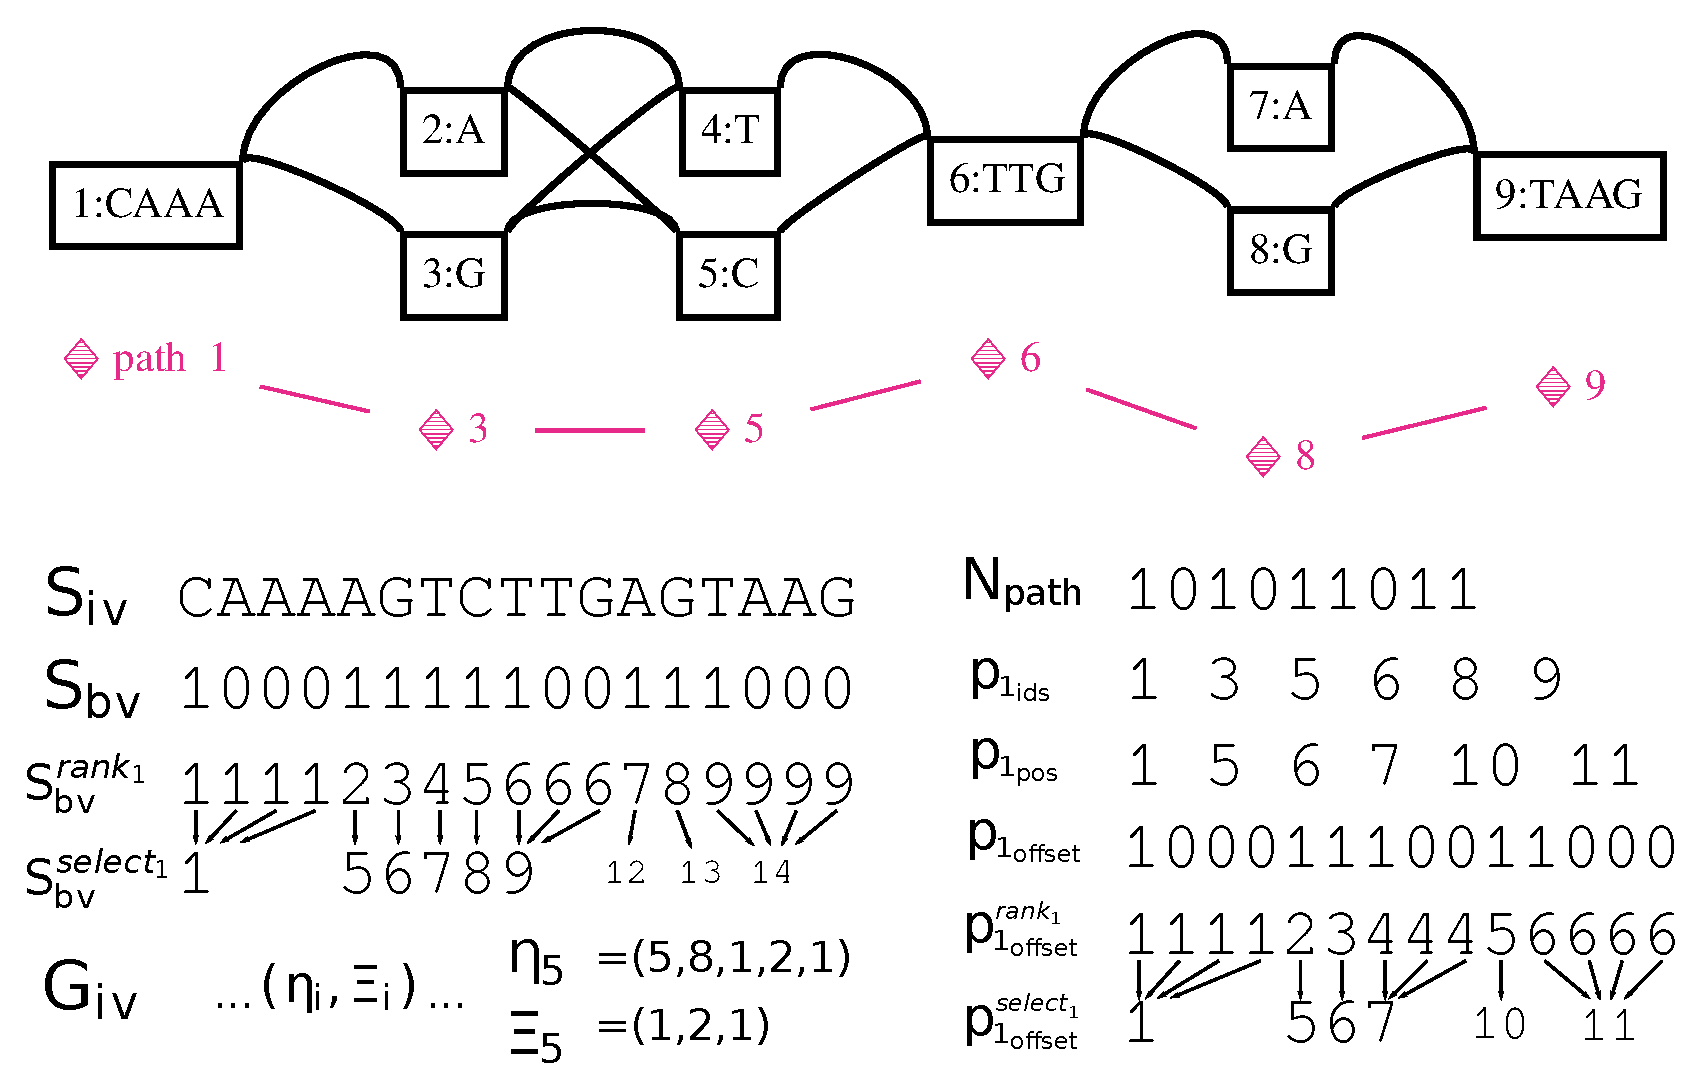
\includegraphics[width=\textwidth]{Chapter2/Figs/xg_index_sketch_nice.pdf}
  \caption[A sketch of the XG index]{
    A visual presentation of the key elements of the XG index for the given graph.
  }
  \label{fig:xg_index}
\end{figure}

To enable better compression, the node sequence space is recorded as a concatenation of node labels $S_\textbf{iv} = seq(n_i) \ldots seq(n_{|N|})$, in which each node has an offset in this sequence space defined by $seq_\textbf{offset}(n_i)$.
In bitvector $S_\textbf{bv} : |S_\textbf{bv}| = |S_\textbf{iv}|$ we set 1 at each first character in a node label, and 0 otherwise: $S_\textbf{bv}[i] = 1 \iff \exists j : seq_\textbf{offset}(n_j) = i \lor 0$.
Random access by node rank $i$ is provided by function $S_\textbf{bv}^{select_1}$, allowing us to find the sequence given a node rank in $G_\textbf{iv}$.

Each $\eta_i$ records node contextual information, including an external id, its offset in the sequence vector, and the degree of $n_i$ in terms of inbound and outbound nodes: $\eta_i = \left[ id(i), seq_\textbf{offset}(n_i), |seq(n_i)|, in(n_i), out(n_i) \right]$.
The use of an external identifier allows the index to work on subsets of larger graphs, and the information about node degree allows us to parse the edge records and efficiently traverse $G_\textbf{iv}$.

The edge context $\Xi_i$ enumerates the set of edges that connect to this node in a structured way that allows for oriented traversals across the two strands of the graph.
To enable fast traversal we rewrite the edges in terms of relative positions in the encoded $G_\textbf{iv}$ vector, which is stored as a bitcompressed integer vector using SDSL-lite's template primitives.
Each node record is stored contiguously.
We delimit the records by a secondary bitvector $G_\textbf{bv}$, for which we build supports for functions $G_\textbf{bv}^{rank_1}$ and $G_\textbf{bv}^{select_1}$, which allow random access of $G_\textbf{iv}$ by node $id$.
Previous designs decomposed the graph structure into a set of parallel vectors, but this required multiple select queries during traversal and provided poor cache locality and performance.

Node to path membership is recorded in an integer vector $N_\textbf{path}$, which contains a contiguous record of path ids that cross each node.
Random access to $N_\textbf{path}$ is provided by a rank/select dictionary built on a bitvector delimiting the various node path membership lists.
Nodes with no path membership are marked in $N_\textbf{path}$ with a 0.

Each path is represented in a set of succinct data structures that let us walk the path by starting at a particular node, query the path position of a given node, or find the node at a particular path position.
We store the path $p_i = m_1 \ldots m_{|p_i|}$ by decomposing its mappings into the nodes (id and orientation) it traverses $p_{i_\textbf{ids}} = id(n_j) \forall n_j \in p_i$ and $p_{i_\textbf{dir}}$ such that $p_{i_\textbf{dir}}[j] = 0 \iff m_j = (n_j, \ldots) \lor 1 \iff m_j = (\overline{n_j}, \ldots)$.
To allow rank and select queries on the node ids, we can store $p_{i_\textbf{ids}}$ in a wavelet tree, although in practice performance is greatly improved by also recording a minimum node id, which decreases the alphabet size and thus memory and runtime costs of the wavelet tree.
So that we may transform nodes to path positions, we use an integer vector to store a path position for each node traversal in the path, $p_{i_\textbf{pos}}$.
To go from path offset to node, we build a bitvector that marks the beginning of each node traversal in the path in a manner similar to that used to mark the sequence beginning of each node in $S_\textbf{iv}$, such that $p_{i_\textbf{offset}}$ is a bitvector of length $\sum_{j=1}^{|p_i|} |seq(p_i[j])|$ where we have marked 1 for each node start in the path, $p_{i_\textbf{offset}}[j] = \left( 1 \iff \exists n_k \in p : j = \sum_{m=1}^{k} |seq(p_i[m])| \right) \lor 0$.
By implementing $p_{i_\textbf{offset}}^{rank_1}$ we can find the node at a given path position $\mathcal{Q}$ by $p_{i_\textbf{offset}}^{rank_1}(\mathcal{Q}) \to j : \left( \sum_{k=1}^{j} |seq(p_i[k])| \leq \mathcal{Q} \land \sum_{k=1}^{j+1} |seq(p_i[k])| > \mathcal{Q} \right)$.
We can also find the position of the $j$th node in a path as $p_{i_\textbf{offset}}^{select_1}(j)$.
A compressed suffix array (CSA) and rank dictionary $P_\textbf{csa}$ and $P_\textbf{name}^{rank_1}$ map from path name to internal rank of the path in $P$.

A number of compression techniques can be applied to the data models in XG to reduce the size of the overall index without any loss in functionality.
However, many of these compression methods producing compressed bitvectors, integer vectors, and wavelet trees, will result in slower access.
In the context of read alignment, such losses may be undesirable as long as there is sufficient memory to load the entire index into system memory, and so I have tuned the index by choosing compression strategies appropriate for its use on current datasets.

\subsection{Graph sequence indexes}
\label{sec:graph_sequence_indexes}
%*1p 2h*
\DIFaddbegin 

\DIFadd{As I presented in section \ref{sec:sequence_alignment}, sequence alignment is driven by sequence indexes that allow efficient queries of subsequences in a given corpus (for instance a reference genome, or a set of reads).
Two main varieties have proved useful.
In $k$-mer indexes, short subsequences of length $k$ are recorded in a hash table or equivalent data structure that allows efficient lookup.
The keys in this table are the $k$-mers, whel the values are typically a list of strand-oriented positions in the target set of sequences.
BWT-based indexes emulate the suffix tree of their input text in small space, and allow $O(l)$ time queries for sequences of length $l$, irrespective of the size of the target corpus.
Implementations of the popular FM-index \mbox{%DIFAUXCMD
\cite{fmindex2000,fmindex2005} }\hspace{0pt}%DIFAUXCMD
and the functionally equivalent compressed suffix array (CSA) \mbox{%DIFAUXCMD
\cite{grossi2005compressed} }\hspace{0pt}%DIFAUXCMD
compress the BWT using encodings that allow fast decompression or direct operation on the compressed data (such run-length compression, or that of Raman, Raman, and Rao \mbox{%DIFAUXCMD
\cite{raman2002succinct}}\hspace{0pt}%DIFAUXCMD
, and augment the BWT with positional information that allows the index to be used for substring matching.
}

\DIFaddend Indexing the sequence space of \DIFdelbegin \DIFdel{a variation graph can be achieved using the same }\DIFdelend \DIFaddbegin \DIFadd{variation graphs requires a generalization of the principles behind these indexing techniques.
Junctions allow for the representation of alternative sequences, with an exponential size relative to the number of furcations in the graph.
This introduces problems of representation and scale which have required substantial work to resolve.
In }{\tt \DIFadd{vg}}\DIFadd{, I was ultimately able to use and encourage the development of a practical implementation of a succinct data structure akin the the CSA, but generalized to operate in any kind of bidirectional sequence graph, the GCSA2.
This this model was developed within the context of }{\tt \DIFadd{vg}}\DIFadd{, and is the first sequence index specifically designed to work on variation graphs.
Here, I will provide a description of related data structures from which this model draws inspiration, as well as a careful summary of the GCSA2 and the features which make it ideal as the core sequence index to drive for a short read to variation graph mapper.
Due to space, I will not fully elaborate this model, as it is not among my contributions.
Readers are encouraged to examine the cited works if they seek a complete description of this and related data structures.
}

\subsubsection{\DIFadd{Graph $k$-mer indexes}}

\DIFadd{It is straightforward to construct a }\DIFaddend $k$-mer \DIFdelbegin \DIFdel{based techniques frequently used in pairwise alignment}\DIFdelend \DIFaddbegin \DIFadd{index of a variation graph.
We simply enumerate the $k$-length walks through the sequence space of the graph.
Problematically, the $k$-mer space of a graph can grow exponentially where variant bubbles cluster within the given length $k$.
To mitigate this issue, we can short-circuit the $k$-mers enumeration when a given number of edges are crossed within $k$ characters.
Another way to mitigate the limitations posed by the exponential number of $k$-mers in the graph is to build the index on disk, rather than using main memory}\DIFaddend .
In the early stages of \DIFdelbegin \DIFdel{this }\DIFdelend \DIFaddbegin \DIFadd{the }{\tt \DIFadd{vg}} \DIFaddend project, I implemented a $k$-mer based index using a disk-backed system (see section \ref{sec:generic_disk_backed_indexes}).
\DIFdelbegin \DIFdel{An efficiently-built in-memory index of }\DIFdelend \DIFaddbegin \DIFadd{By sorting the }\DIFaddend $k$-mers, \DIFdelbegin \DIFdel{perhaps sampled and possibly $w,k$-minimizers \mbox{%DIFAUXCMD
\cite{marccais2018asymptotically,li2018minimap2}}\hspace{0pt}%DIFAUXCMD
, appears to be a reasonable basis for a sequence to graph aligner, but I did not explore this beyond these initial experiments.
Our research focus on the replication of results of the short read mapper }\DIFdelend \DIFaddbegin \DIFadd{the index could be efficiently compressed, but still the graph for the human 1000 Genomes Project required over 200GB of memory, and was unusably slow unless cached in main memory.
This index formed the basis for the first prototypes of the }\DIFaddend {\tt \DIFdelbegin \DIFdel{bwa mem}\DIFdelend \DIFaddbegin \DIFadd{vg}\DIFaddend } \DIFdelbegin \DIFdel{, which seeds alignments with maximal exact matches (MEMs), encouraged a similar approach for }\DIFdelend \DIFaddbegin \DIFadd{mapper, but is be impractical due to its time and memory requirements.
}

\subsubsection{\DIFadd{The FM-index and Compressed Suffix Array (CSA)}}
\label{sec:fmidx_csa}

\DIFadd{As introduced in section \ref{sec:compressed_full_text_indexes}, compressed full text self indexes like the CSA and equivalent FM-index provide functionality similar to that of the suffix tree (as in Figure \ref{fig:suffix_tree}) but in compressed space.
The functionality of these indexes is the basis for the indexing techniques applied in }\DIFaddend {\tt vg} \DIFdelbegin \DIFdel{.
MEMs are found using a suffix tree related data structure, which provides access to a wide range of efficient sequence matching and inference algorithms, and a strong basis for a sensitive read aligner}\DIFdelend \DIFaddbegin \DIFadd{to the alignment of reads to variation graphs.
Here, I will first illustrate the construction of a full text index based on the Burrows Wheeler transform (BWT) and suffix array (SA), and show how it can be used to locate occurrences of a pattern in the source text.
This discussion will form the basis for an elaboration of the generalizations that lead to a similar kind of index built over a variation graph}\DIFaddend .

\DIFdelbegin \DIFdel{On seeing my early experiments, Jouni Sir\'{e}n, who had recently joined our lab, suggested that there might be a way to adjust his GCSA index model for partially ordered graphs to work on arbitrary graphs.
He proposed a de Bruijn graph (DBG)transformation of }\DIFdelend \DIFaddbegin \begin{figure}[htbp!]
  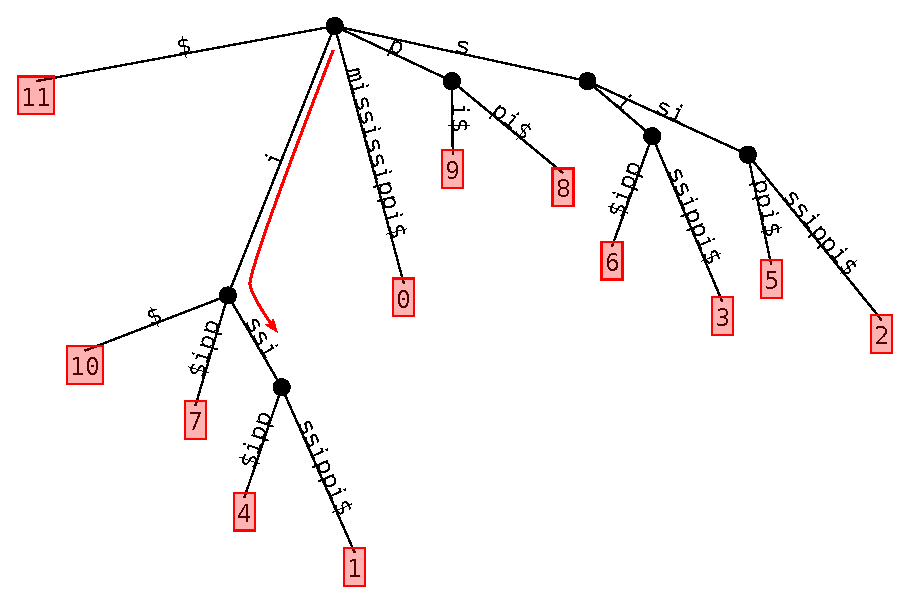
\includegraphics[width=\textwidth]{Chapter2/Figs/mississippi_suffix_tree.pdf}
  \caption[An example of a suffix tree]{
    \DIFaddFL{A suffix tree built from the suffixes of the string }{\tt \DIFaddFL{mississippi}}\DIFaddFL{.
    Suffixes begin at the root, shown at the top.
    Leaves are labeled by their suffix, which is written in terms of the 0-based starting position of the suffix in the source text.
    A red arrow shows a search for the string ``iss'' on the tree.
    The leaves of the tree below the ultimate point reached by this search give the positions of the matched pattern in the source text, in this case 1 and 4.
    Rendered with }\url{https://github.com/mpetri/draw-suffix-tree}\DIFaddFL{.
  }}
  \label{fig:suffix_tree}
\end{figure}

\DIFadd{To construct the BWT from a given string $T$, we first append a marker character that is outside the alphabet (e.g. }{\tt \DIFadd{\$}}\DIFadd{) to the text.
We take all rotations of this string, and lexicographically order them to form a matrix, which is sometimes referred to as the Burrows Wheeler matrix (BWM).
The first column of this matrix is $F$, and lists the characters in the source text in lexicographic order.
We can compactly represent it as a vector of counts $C$ of characters that are lexicographically smaller than a given one, indexed by the characters as encoded in a compact set of integers.
The last column of the BWM is the Burrows Wheeler transform (BWT) of the source text.
The order in which the rotations (or equivalently, suffixes) appear in the sort is the suffix array (SA) of the text
Assume a function $rank_{BWT}(c, i)$ which returns the number of characters equal to $c$ in }\DIFaddend the \DIFdelbegin \DIFdel{graph as input to the indexing process.
The resulting indexing model is similar to both GCSA, in its encoding of the graph topology, and succinct DBGs \mbox{%DIFAUXCMD
\cite{bowe2012succinct}}\hspace{0pt}%DIFAUXCMD
, which are also developed from BWTs based on a $k$-mer set.
Sir\'{e}n's design allows for the use of much longer $k$-mers than are typically considered in DBGs, with the final DBG to be indexed having $k=256$.
As few contemporary reads are likely to generate 256bp-long sequences with no mismatch from the reference}\footnote{\DIFdel{Illumina's reads rarely reach 256bp, and when they do they tend to have higher error rates in the later cycles. The 10-15\% error rate of PacBio and ONT sequencing mean that a 256bp exact match is extremely unlikely, although PacBio circular consensus reads (CCR) may approach this level of accuracy.}}%DIFAUXCMD
\addtocounter{footnote}{-1}%DIFAUXCMD
\DIFdel{, this approach effectively allows us to find all the exact matches for a typical sequencing read.
To be more precise, we find supermaximal exact matches (SMEMs) as defined in \mbox{%DIFAUXCMD
\cite{li2013aligning}}\hspace{0pt}%DIFAUXCMD
.
}\DIFdelend \DIFaddbegin \DIFadd{prefix of $BWT[0\ldots i]$.
The function $LF(i) = C[c] + rank_{BWT}(c, i) - 1$ reconstructs the mapping between the same character in the BWT and $F$, thus provides a way to unwind the permutation generated by the sort and reconstruct the source text.
These construction steps are illustrated in Figure \ref{fig:bwt_construction}.
}

\begin{figure}[htbp!]
  \centering
  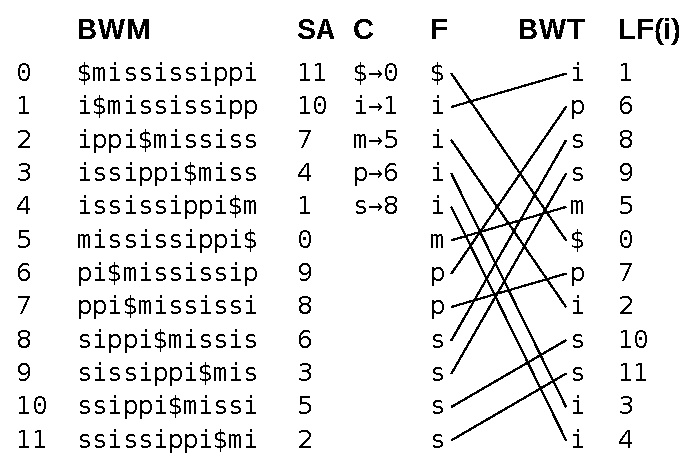
\includegraphics[width=0.65\textwidth]{Chapter2/Figs/mississippi_bwt_construction.pdf}
  \caption[Building the BWT and suffix array]{
    \DIFaddFL{A BWT and suffix array built from the string }{\tt \DIFaddFL{mississippi}}\DIFaddFL{.
    The Burrows Wheeler Matrix (BWM) shows all rotations of the string (appended with terminal marker }{\tt \DIFaddFL{\$}}\DIFaddFL{) in lexicographical order.
    $SA$ provides the suffix array, which lists the suffixes relative to the original string in their sorted order in the BWM.
    The first column of the BWM corresponds to vector $F$, which contains a series of runs of single characters in their lexicographic order, and is compactly represented in $C$.
    The last column of the BWM corresponds to the $BWT$.
    The function $LF(i)$ is shown for each position in the $BWT$, and lines drawn between $F$ and $BWT$ show the characters in the system that have the same identity in the source text.
    Produced using }\url{https://github.com/ekg/drawbwt}\DIFaddFL{.
  }}
  \label{fig:bwt_construction}
\end{figure}

\DIFadd{We can use $LF$ mapping in an iterative way to execute search on the BWT.
Algorithm \ref{alg:bwt_find} defines the function $find(Q)$, which returns the suffix array interval (or lexicographic range) in which suffixes are prefixed by $Q$, should it exist, and an empty interval if $Q$ is not a substring of $T$.
We begin our search by looking at the SA interval prefixed by the last character in our pattern, which is trivially obtained from array $C$.
The body of the loop constitutes one step of backward searching.
Searching works by maintaining the invariant that the prefix of the suffixes in the SA interval defined by $[sp, ep]$ is that given by the set of characters that we have considered in reverse order from the query string $Q$.
}

\begin{algorithm}
  \caption[BWT find]{
  \DIFadd{Backward searching on the BWT
  }}
  \label{alg:bwt_find}
  \begin{algorithmic}
    \Function{find}{Q}
    \State \DIFadd{$c \gets Q[|Q|-1]$ }\Comment{Current character in our search}
    \State \DIFadd{$sp \gets C[c]$ }\Comment{Beginning of our SA interval}
    \State \DIFadd{$ep \gets C[c+1]-1$ }\Comment{End of our SA interval}
      \For{$i \in [|Q|-2 \ldots 0]$} \Comment{Step backwards through the string}
        \State \DIFadd{$c \gets Q[i]$ }\Comment{Update our character}
        \State \DIFadd{$sp \gets C[c] + rank_{BWT}(c, sp - 1)$ }\Comment{Update $sp$ dependent on $c$}
        \State \DIFadd{$ep \gets C[c] + rank_{BWT}(c, ep) - 1$ }\Comment{Do the same for $ep$}
        \If{$sp > ep$} 
          \Return{$\emptyset$}  \Comment{We do not find $Q$ in our text}
        \EndIf
      \EndFor \\
      \Return{$[sp, ep]$} \Comment{Return the SA interval prefixed by $Q$}
    \EndFunction
  \end{algorithmic}
\end{algorithm}


\begin{figure}[htbp!]
  \centering
  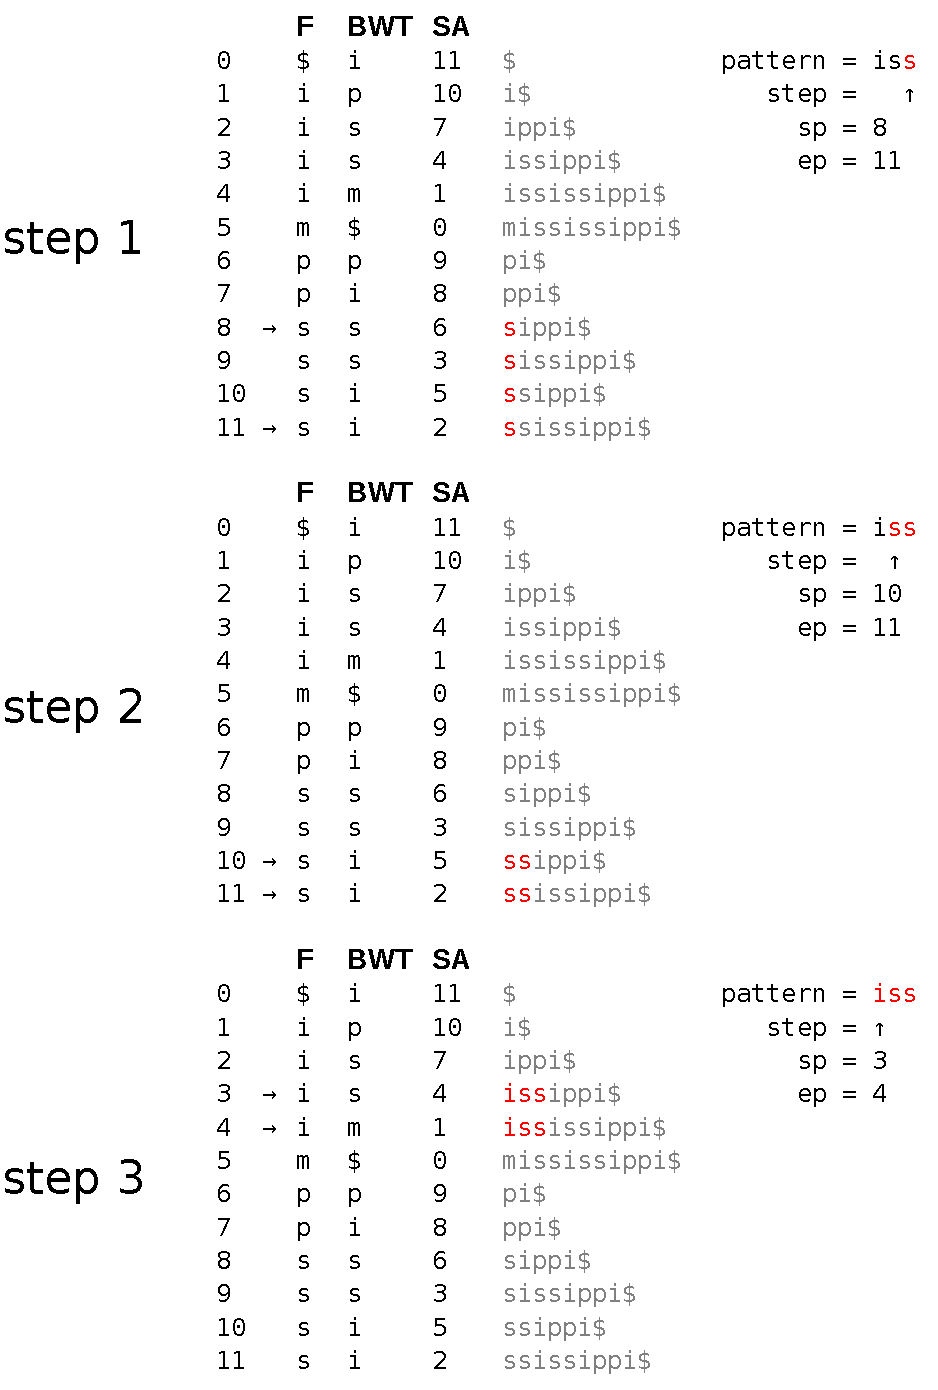
\includegraphics[width=0.65\textwidth]{Chapter2/Figs/mississippi_iss_search.pdf}
  \caption[Backward search in the BWT and suffix array]{
    \DIFaddFL{Using backward search to find all occurrences of }{\tt \DIFaddFL{iss}} \DIFaddFL{in }{\tt \DIFaddFL{mississippi}}\DIFaddFL{, using the BWT and suffix array constructed in Figure \ref{fig:bwt_construction}.
    The index structure is shown in each of the three required steps (1$\to$3), which progress from top to bottom.
    At each step, we consider a character, beginning from the end of the string we are searching.
    We apply $LF$ mapping to find the new SA interval corresponding to the backwards extension of our query pattern.
    The subsequence matched up to the current step is shown in red in the sorted suffixes (in gray) represented by $F$, $BWT$, and $SA$.
    We do not store these sorted suffixes, as they are given by the $BWT$ and $SA$.
    Nor do we store $F$, as the $C$ array is sufficient to reconstruct it.
    Rendered with }\url{https://github.com/ekg/drawbwt}\DIFaddFL{.
  }}
  \label{fig:bwt_search}
\end{figure}

\DIFaddend The addition of the longest common prefix (LCP) array \DIFdelbegin \DIFdel{alongside GCSA2's BWT effectively generalizes all essential operations on a suffix tree to the GCSA2, and enables us to find SMEMs and develop sensitive MEM-based seeding heuristics using the index.
The design of GCSA2 is wholly Sir\'{e}n's work \mbox{%DIFAUXCMD
\cite{siren2017indexing}}\hspace{0pt}%DIFAUXCMD
, and it forms one of the core components of the }\DIFdelend \DIFaddbegin \DIFadd{on the sorted suffixes allows the CSA to emulate all algorithms on suffix trees \mbox{%DIFAUXCMD
\cite{abouelhoda2004replacing}}\hspace{0pt}%DIFAUXCMD
.
This augmented data structure provides a compact encoding of the full suffix tree topology.
In }\DIFaddend {\tt vg}\DIFdelbegin \DIFdel{mapper paper, which we coauthored.
I present it here because the mapping algorithm I developed for }\DIFdelend \DIFaddbegin \DIFadd{, an equivalent generalization is used to enable the determination of maximum exact matches between query $P$ and the sequences of a graph.
}


\subsubsection{\DIFadd{BWT-based tree and graph sequence indexes}}

\DIFadd{In contrast to $k$-mer based indexes, generalizations of the CSA to graphs have required substantial conceptual developement to produce.
But, they have yielded compact, efficient data structures that require similar space to their linear counterparts while supporting a wide array of query patterns.
}

\DIFadd{Most generalizations of succinct self indexes from strings to graphs draw on the XBW transform \mbox{%DIFAUXCMD
\cite{ferragina2005structuring}}\hspace{0pt}%DIFAUXCMD
, which provides a compressed self index of trees based on a generalization of the FM-index \mbox{%DIFAUXCMD
\cite{ferragina2009compressing}}\hspace{0pt}%DIFAUXCMD
.
In the XBW transform (figure \ref{fig:xbw}), rather than considering all suffixes of a linear sequence in the construction of the BWT, we sort all concatenated paths from the root to leaves of each node in the tree and use this as the basis for the BWT in a manner analagous to the use of sorted suffixes for a linear sequences.
To record the topology of the tree and support its navigation relative to the resulting BWT, auxiliary bitvectors record which edges connect to leaf nodes $e$ (or equivalently, an expanded alphabet as originally presented in \mbox{%DIFAUXCMD
\cite{ferragina2005structuring}}\hspace{0pt}%DIFAUXCMD
), and which are the last edge among their siblings: ${\cal F}$.
Rank and select queries on these bitvectors allow the generalization of the }\emph{\DIFadd{LF-mapping}} \DIFadd{(last-first) permutation and its inverse $\Psi$ to work on the tree.
The lexicographic ranks of the standard versions of these functions are mapped into the appropriate BWT ranges using rank and select queries on ${\cal F}$.
}


\begin{figure}[htbp!]
  \centering
  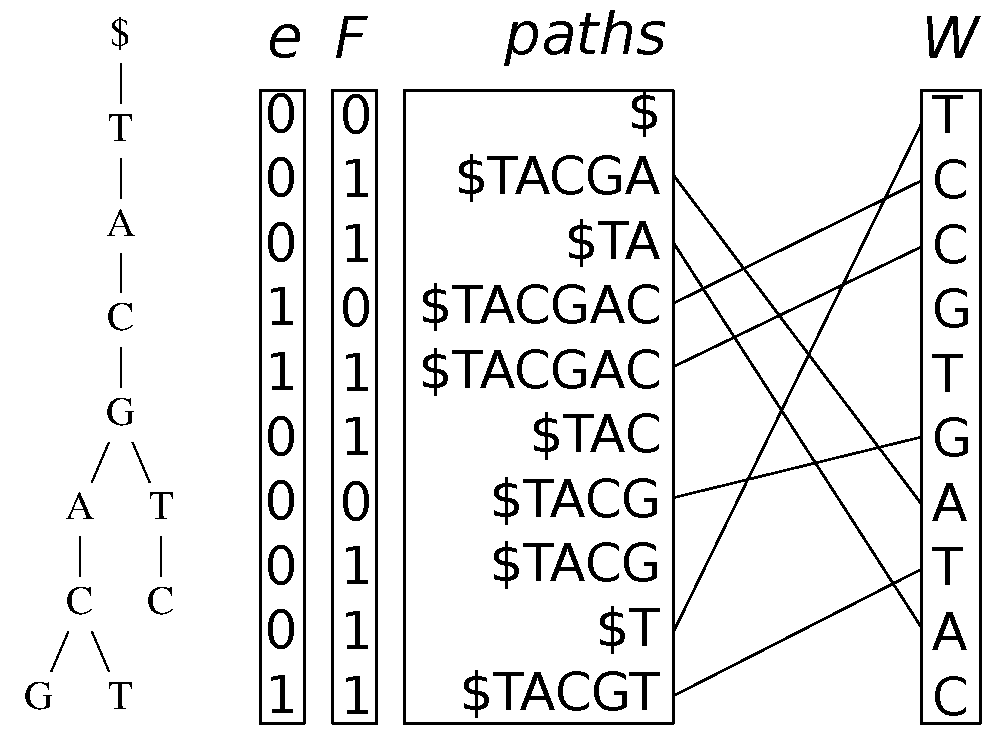
\includegraphics[width=0.6\textwidth]{Chapter2/Figs/xbw_viz.pdf}
  \caption[The XBW transform]{
    \DIFaddFL{The XBW transform and the $LF$ function computed for the given graph.
    Nodes are stored in $W$, while bitvector $e$ marks the leaf nodes (whose LF mapping is $\emptyset$), and bitvector ${\cal F}$ marks the last nodes in each set of siblings.
    By construction, siblings are sorted together in the set of sorted paths.
    Paths are not stored, but are shown here for clarity.
    Example adapted from a public talk by Alex Bowe, posted at }\url{https://pdfs.semanticscholar.org/e42a/daab2806d5c0d715cb812c3a10aa26a2c75a.pdf}\DIFaddFL{.
  }}
  \label{fig:xbw}
\end{figure}


\DIFadd{Succinct deBruijn graphs (SDBG) extend the XBW model to support DBGs by recording both in and out degree for each node \mbox{%DIFAUXCMD
\cite{bowe2012succinct,muggli2017succinct}}\hspace{0pt}%DIFAUXCMD
.}\footnote{\DIFadd{See }\url{https://alexbowe.com/succinct-debruijn-graphs/} \DIFadd{for a high-level overview of Bowe's initial model for succinct DBGs, which explains in detail how the various graph traversal and query operations are implemented.}}
\DIFadd{In }\DIFaddend {\tt vg}\DIFdelbegin \DIFdel{relies on it heavily}\DIFdelend \DIFaddbegin \DIFadd{, we do not use the SDBG model directly, but it is important to describe here as the GCSA2 model draws heavily on its design}\DIFaddend .

To \DIFdelbegin \DIFdel{reduce redundancy, GCSA2 uses a }\emph{\DIFdel{pruned DBG}} %DIFAUXCMD
\DIFdel{whose nodes may have labels shorter than }\DIFdelend \DIFaddbegin \DIFadd{construct the SDBG (illustrated in figure \ref{fig:sdbg}), we build two sorted lists of tuples representing the edge and }\DIFaddend $k$\DIFdelbegin \DIFdel{where these shorter strings still uniquely identify the beginning of their corresponding paths in the unpruned DBG.
}\DIFdelend \DIFaddbegin \DIFadd{-mer space of the DBG $G = (N, E)$.
First, we pad the graph with additional nodes labeled by a character lexicographically lower than the alphabet of the graph, so that each $k$-mer in $G$ is now reachable from a path at least $k-1$ long.
This ensures that we can reconstruct the graph without loss.
In $F$, we record the list of $G$'s edges sorted co-lexicographically by the reverse sequence of their }\emph{\DIFadd{ending}} \DIFadd{node and their label.
In $L$, we record the list of $G$'s edges sorted co-lexicographically by the reverse sequence of their }\emph{\DIFadd{starting}} \DIFadd{node and their label.
The edge-BWT (EBWT) is the sequence of edge labels as given in $L$.
}

\DIFadd{Navigation of the graph is provided by the mapping between $F$ and $L$ that is based on the relative stability of sorting of edges with the same label in the two lists.
If an edge $e$ is in position $p$ in $L$, and $l(e)$ is a function that gives the character label of edge $e$, then its position in $F$ is given by $|{d : d \in E \land l(d) \prec l(e)}| + rank_{EBWT}(l(e), p) - 1$.
Note that this function corresponds to $LF$ mapping on the BWT.
A similar extension of this idea affords backward search of patterns in node labels in the SDBG.
For full navigation, we must edge topology bitvectors $B_F$, which marks the last edge for each node in $F$, and $B_L$, which does the same for $L$.
We can traverse the graph using these structures.
Given a character $c$ and the co-lexicographic rank of a node, we can use $B_L$ to find the interval in $L$ containing its node's outgoing edges, then find the edge $e$ labeled $c$ in the $EBWT$, and finally use $B_F$ to find the co-lexicographic rank of $e$'s ending node, should it exist.
}\DIFaddend 

\begin{figure}[htbp!]
  \DIFdelbeginFL %DIFDELCMD < 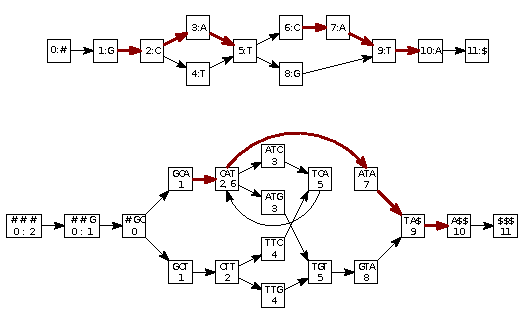
\includegraphics[width=\textwidth]{Chapter2/Figs/sequence_graph_to_DBG.pdf}
%DIFDELCMD <   %%%
%DIFDELCMD < \caption[A sequence graph and its de Bruijn transformation]{%
{%DIFAUXCMD
\DIFdelFL{A sequence graph and its de Bruijn transformation.
    Reprinted from \mbox{%DIFAUXCMD
\cite{siren2017indexing}}\hspace{0pt}%DIFAUXCMD
.
  }}
  %DIFAUXCMD
%DIFDELCMD < \label{fig:seq_graph_to_dbg}
%DIFDELCMD < %%%
\DIFdelendFL \DIFaddbeginFL \centering
  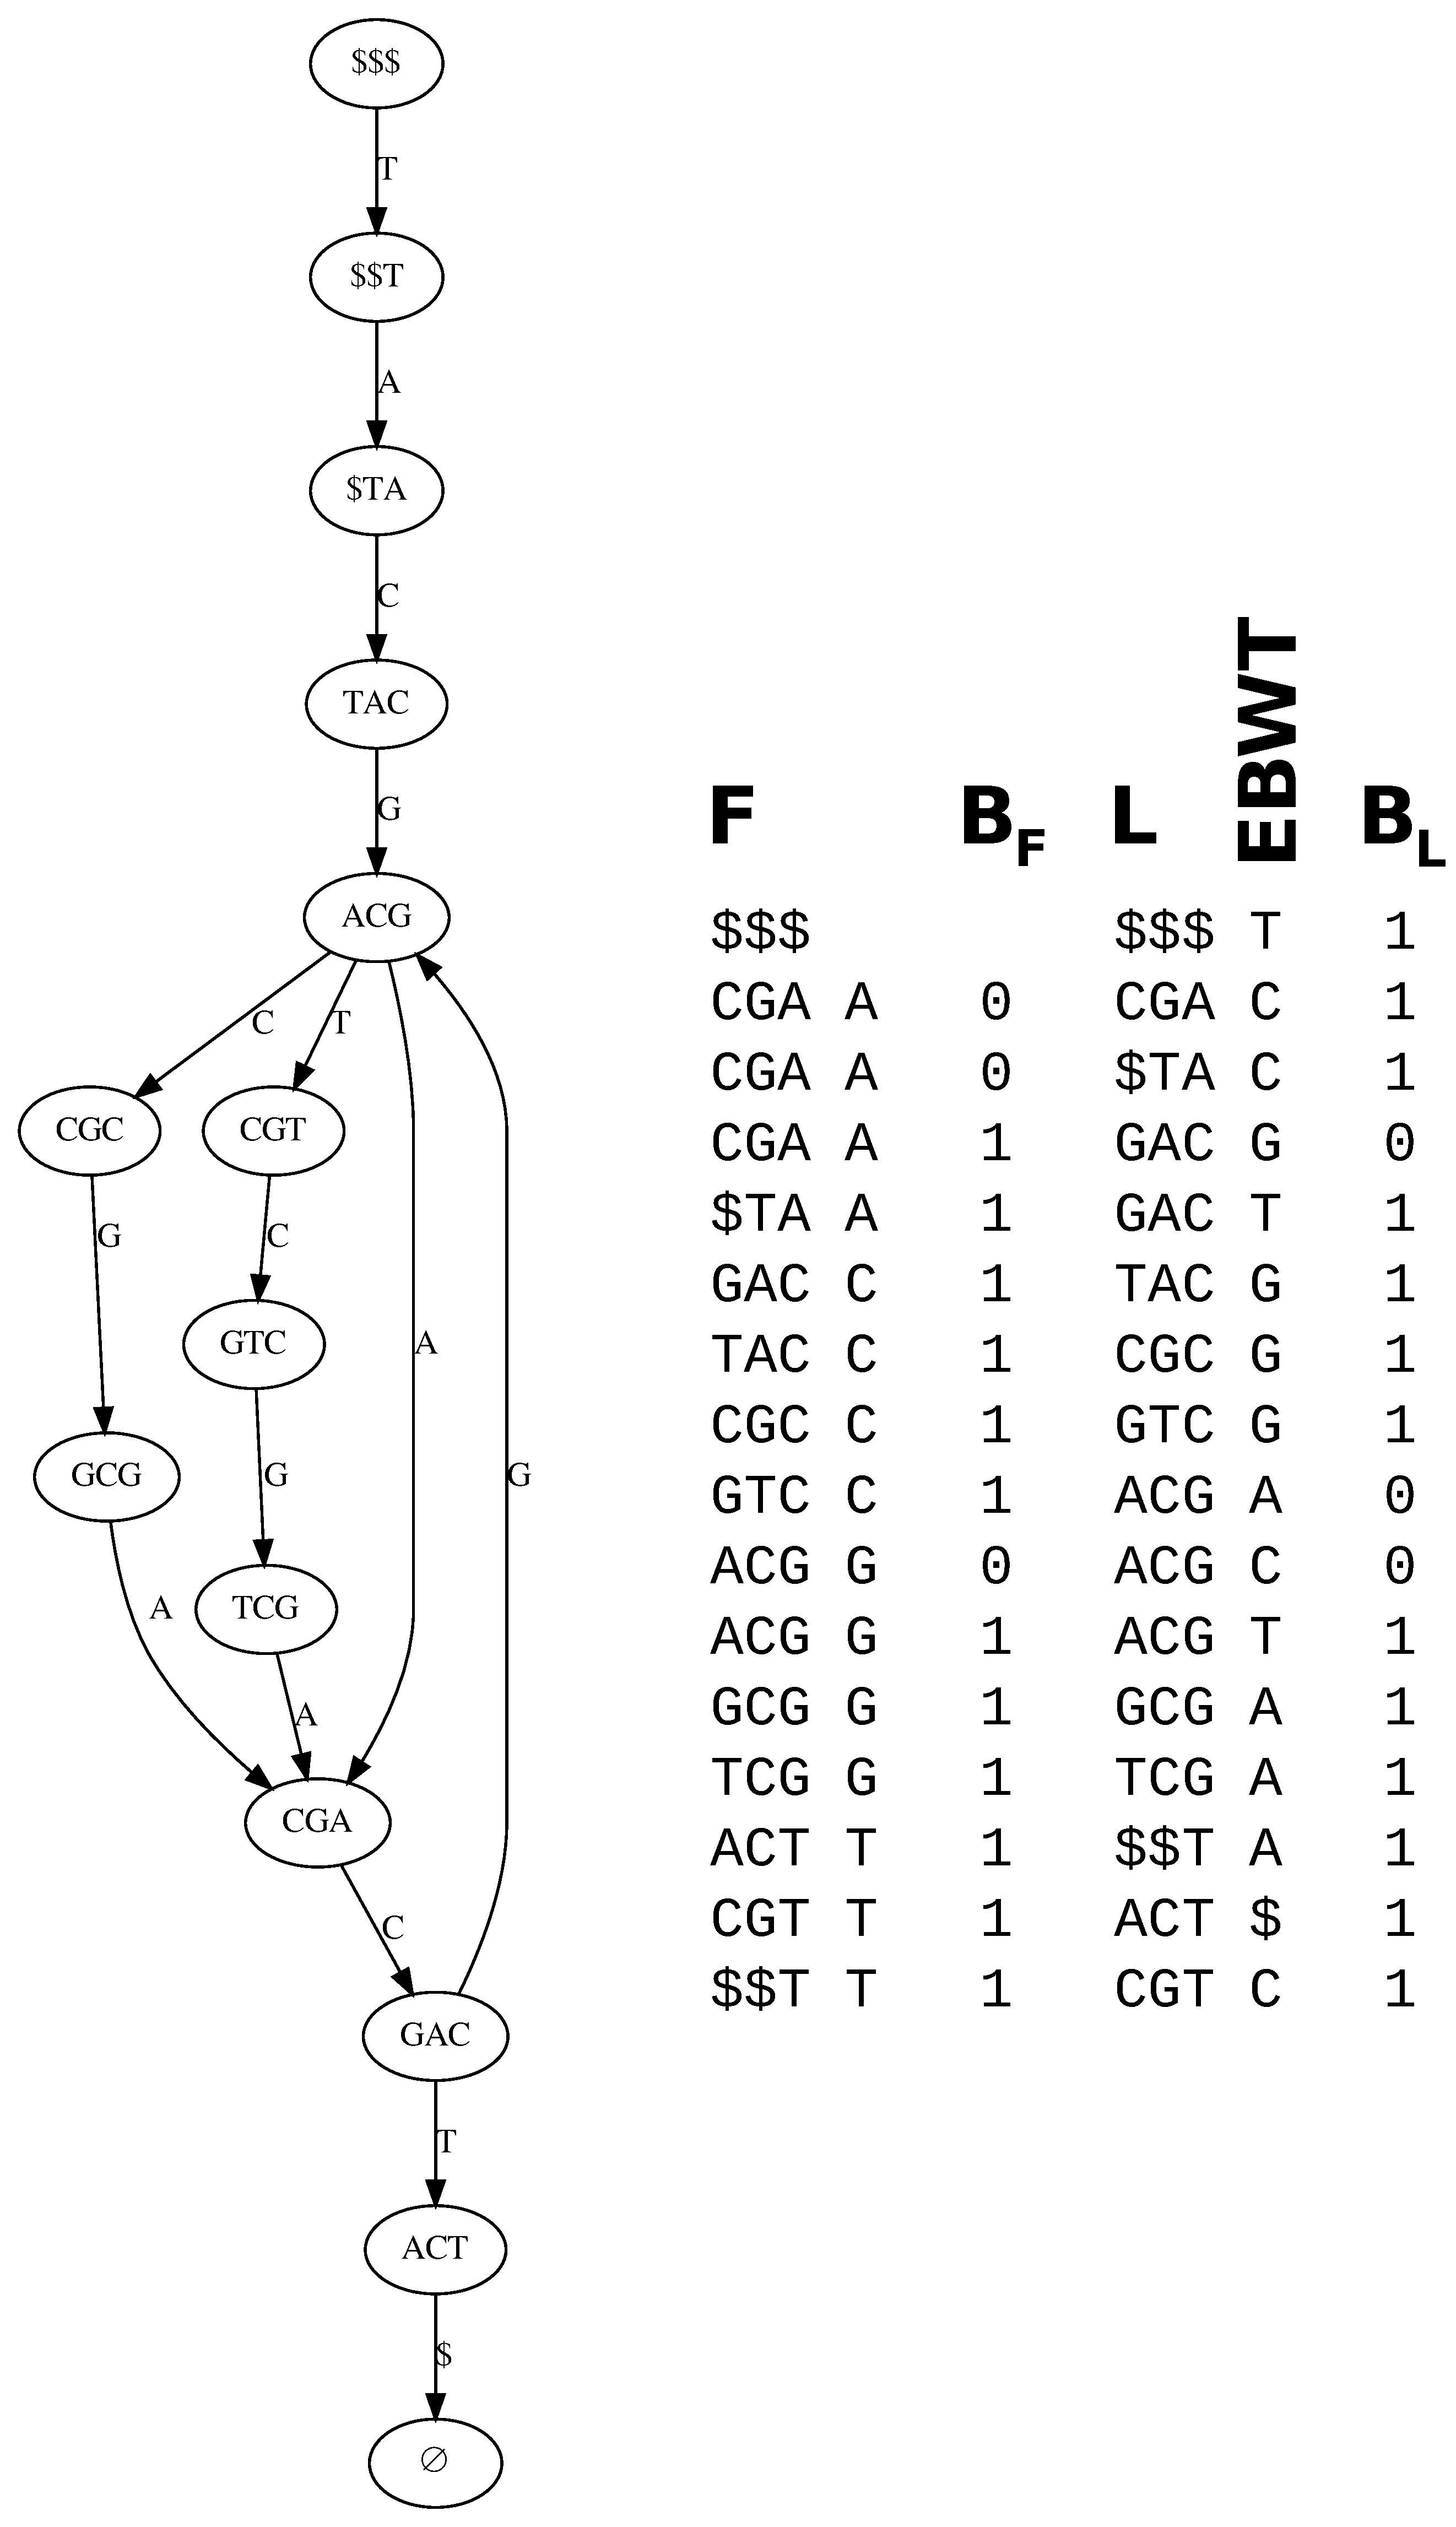
\includegraphics[width=0.65\textwidth]{Chapter2/Figs/sdbg_construction.pdf}
  \caption[Succinct de Bruijn graph construction]{
    \DIFaddFL{On the left, a de Bruijn graph with $k=3$, with edges labeled by the character transition that they imply.
    Right, the construction of the succinct de Bruijn graph for the given graph.
    $F$ indicates the co-lexicographically sorted set of edges keyed by the node that they enter.
    $L$ indicates the co-lexicographically sorted set of edges keyed by the node that they leave.
    $B_{F}$ marks if the edge in $F$ is co-lexicographically the last for its corresponding node, and $B_{L}$ marks the last edge for a given node in $L$.
    The ``edge BWT'' or $EBWT$ is given as the set of edges ordered as in $L$.
    The SDBG is given by $B_F$, $B_L$, and $EBWT$.
    Example adapted from \mbox{%DIFAUXCMD
\cite{muggli2017succinct}}\hspace{0pt}%DIFAUXCMD
.
  }}
  \label{fig:sdbg}
\DIFaddendFL \end{figure}
\DIFdelbegin %DIFDELCMD < 

%DIFDELCMD < %%%
\DIFdel{This pruned graph is then encoded in a generalization of the }\DIFdelend \DIFaddbegin 


\subsubsection{\DIFadd{The Generalized Compressed Suffix Array}}

\DIFadd{In section \ref{sec:pangenomic_sequence_indexes}, I discuss a variety of indexing models that support indexing reference genomes and variants.
Many schemes are possible, but the first to provide a conceptually complete solution to the problem of establishing a sequence index for a structure similar to a variation graph is Sir\'{e}n's Generalized Compressed Suffix Array (GCSA) \mbox{%DIFAUXCMD
\cite{siren2014indexing}}\hspace{0pt}%DIFAUXCMD
.
This structure allows for queries of arbitrary length within a directed, acyclic variation graph (equivalently, a finite language model or MSA) in much the same way as the }\DIFaddend FM-index \DIFdelbegin \DIFdel{built on a BWT of the $k$-mers in the pruned DBG.
The FM-index is extended to support search over the DBG by adding auxiliary bitvectors which record the indegree and outdegree of nodes in the pruned DBG.
These are used in backwards search to adjust the suffix array ranges that are considered, expanding them when the indegree is greater than 1 and contracting them when the out degree is greater than 1, in effect encoding the graph structure into the index in a space efficient manner optimized for traversal.
This technique is the same as that used in GCSA, although GCSA indexes }\DIFdelend \DIFaddbegin \DIFadd{or CSA do for linear sequences.
}

\DIFadd{To build the GCSA, we first construct a sequence labeled DAG (which Sir\'{e}n describes as a MSA) from the reference and a set of genetic variants.
As in the succinct DBG, we attach marker nodes to the graph for its head and tail.
The MSA is converted into }\DIFaddend a reverse deterministic automaton \DIFdelbegin \DIFdel{rather than a DBG.
Impressively, GCSA2 uses around 1 bit per }\DIFdelend \DIFaddbegin \DIFadd{via a standard procedure for determinizing finite state automata.
This results in a structure where there is no more than one of each character in the alphabet among the predecessors of each node.
Recall (section \ref{sec:fmidx_csa}) that backward searching using the BWT requires that positions in the text containing a given character $c$ are sorted in the same order as text positions preceded by character $c$.
Thus, to provide equivalent functionality for an automaton, we must ensure that each node in the automaton will be stably sorted when we enumerate and sort its suffixes.
This implies a transformation of the automaton that ensures that each prefix of a path through the graph is the only way to generate a suffix with the particular prefix.
Sir\'{e}n implements this prefix-sorting transform in an algorithm that }\DIFaddend $k$\DIFdelbegin \DIFdel{-mer in indexes of the 1000GP pangenome graph for $k=128$, which is favorable with comparison to true DBG indexes.
}\DIFdelend \DIFaddbegin \DIFadd{-prefix-sorts the graph for a given $k$.
The process is iterated for $k' = 2k$ until $k'$ is greater than the length of the longest path in the automaton.
At this point, it is possible to enumerate and sort the suffixes of the given automaton, build the corresponding BWT, and augment the data structure with bitvector ${\cal F}$, which allows a single node to have multiple predecessors, and bitvector ${\cal M}$, which records the number of successors or outgoing edges from each nodes in the automaton.
Backward searching in this structure ($LF$) uses a similar principle to the XBW and succinct DBG models.
We first use bitvector ${\cal F}$ to convert lexicographic ranks to a BWT range, and then we use ${\cal M}$ to convert the edge range to lexicographic ranks.
}\DIFaddend 

\DIFdelbegin \DIFdel{As an FM-index like structure, }\DIFdelend %DIF > The GCSA is also an important basis for the GCSA2 model used in {\tt vg}, but for space reasons I will not provide an exhaustive description of it.
%DIF > Although it provides full text queries over a sequence DAG, the GCSA is impractical because to construct it we must enumerate all suffixes of the graph.
%DIF > This requires exponential space with respect to the number of variants in the graph, and renders it unusable for arbitrary inputs.
\DIFaddbegin 

\subsubsection{\DIFadd{GCSA2}}

\DIFadd{Sir\'{e}n's update to GCSA, }\DIFaddend GCSA2\DIFdelbegin \DIFdel{supports queries for a pattern $X$ that yield the suffix array interval matching a given pattern: $find(X) = ( sp_{X}, ep_{X} )$, and $locate( sp_{X}, ep_{X} ) = \{ b_1 \ldots b_{count(sp_{X}, ep_{X})} \}$ which yields the positions in the input VG where the given patterns occur.
The LCP array allows the index to support several operations that require a suffix tree, including $count(sp_i, ep_i)$, which returns the number of matches for a given suffix array range, and $parent(sp_i, ep_i) = (sp_j, ep_j)$, which allows us to traverse the suffix links embedded in the suffix tree and forms the basis of maximal exact match (MEM) inference using }\DIFdelend \DIFaddbegin \DIFadd{, is specifically designed for application to arbitrary variation graphs \mbox{%DIFAUXCMD
\cite{siren2017indexing}}\hspace{0pt}%DIFAUXCMD
.
It is the first index to provide an emulation of the full range of suffix tree operations in the context of a sequence graph.
The crucial observation that drove the development of }\DIFaddend GCSA2 \DIFdelbegin \DIFdel{.
}\DIFdelend \DIFaddbegin \DIFadd{is that it is not necessary to enable full length queries of the graph for a graph path index to be useful.
Shorter graph path queries are fully sufficient as the basis for sequence mapping to the graph, which is the primary application of a graph sequence index.
}\DIFaddend 

\DIFdelbegin %DIFDELCMD < \begin{figure}[htbp!]
%DIFDELCMD <   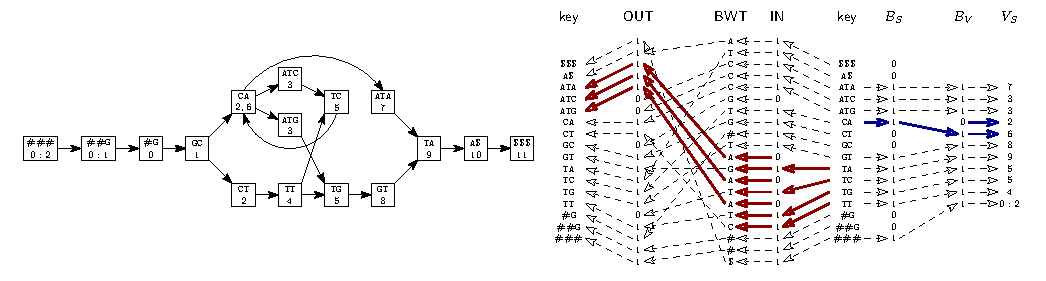
\includegraphics[width=\textwidth]{Chapter2/Figs/DBG_to_GCSA.pdf}
%DIFDELCMD <   %%%
%DIFDELCMD < \caption[Searching in the {\tt GCSA2}]{%
{%DIFAUXCMD
\DIFdelFL{Left: An order-3 pruned de Bruijn graph 3-equivalent to the de Bruijn graph in figure \ref{fig:seq_graph_to_dbg}.
    Right: GCSA for the graph.
    Leftward arrows illustrate backward searching, with the red arrows showing it from }%DIFDELCMD < {\tt %%%
\DIFdelFL{T}%DIFDELCMD < } %%%
\DIFdelFL{to }%DIFDELCMD < {\tt %%%
\DIFdelFL{AT}%DIFDELCMD < }%%%
\DIFdelFL{.
    Rightward arrows mark the samples belonging to each node, with the blue ones showing them for node }%DIFDELCMD < {\tt %%%
\DIFdelFL{CAT}%DIFDELCMD < }%%%
\DIFdelFL{.
    Reprinted from \mbox{%DIFAUXCMD
\cite{siren2017indexing}}\hspace{0pt}%DIFAUXCMD
.
  }}
  %DIFAUXCMD
%DIFDELCMD < \label{fig:gcsa2_search}
%DIFDELCMD < \end{figure}
%DIFDELCMD < %%%
\DIFdelend \DIFaddbegin \DIFadd{GCSA2 brings together ideas from succinct DBGs and the GCSA model.
At a high level, we can consider it to be a compact de Bruijn graph $k$-mer index of a variation graph.
However, in implementation several transformations are required to maintain acceptable bounds on the space required by this model.
The de Bruijn graph is }\emph{\DIFadd{pruned}} \DIFadd{by using strings smaller than $k$ characters as nodes so long as the shorter strings still uniquely identify the corresponding paths in the graph.
GCSA2 transforms the pruned DBG into a BWT, using additional bitvectors $IN$ and $OUT$ analgous to $F$ and $L$ in SDBG to record the graph topology in a generalization of the FM-index.
The full data structure includes extensions to allow suffix tree operations that are important for finding maximal exact matches during sequence search.
}\DIFaddend 

\DIFaddbegin \DIFadd{The }\DIFaddend GCSA2 \DIFdelbegin \DIFdel{resolves a number of problems that limit the utility of other graph path indexing schemes.
Indexing a pruned DBG allows }\DIFdelend \DIFaddbegin \DIFadd{model is more flexible with respect to the complexity of input graphs than GCSA.
}\DIFaddend GCSA2 \DIFaddbegin \DIFadd{uses disk backed construction methods to allow the indexing process to scale to very large graphs.
The $k$-mer length limitation of the index allows it }\DIFaddend to be applied to \DIFdelbegin \DIFdel{arbitrary bidirectional string graphs that include reversals and loops.
It }\DIFdelend \DIFaddbegin \DIFadd{any variation graph, including those that have cycles or other regions of topological compexity, with the caveat that we cannot search for sequences of length greater than $k$ without the risk of finding false positives.
Denser graphs may be indexed by limiting the maximum query length.
The DBG transformation provides flexibility by decoupling the graph we are indexing from the index structure itself.
For instance, edge pruning can be applied to the input graph to remove regions of local complexity, yet it is still possible to generate an index from such fragmented subgraphs because we can always generate a DBG by enumerating $k$-paths through a variation graph.
Unlike competing graph indexing methods, such as BWBBLE and the vBWT (section \ref{sec:pangenomic_sequence_indexes}), GCSA2 }\DIFaddend avoids exponential costs during backwards search.
However, it does incur exponential costs in construction of the index\DIFdelbegin \DIFdel{.
To mitigate the affects of these it may be constructed mostly in external memory, and furthermore construction may be broken into pieces by chromosome or some other subdivision }\DIFdelend \DIFaddbegin \DIFadd{, as it must enumerate all $k$-paths in the graph.
}

\begin{figure}[htbp!]
  \centering
  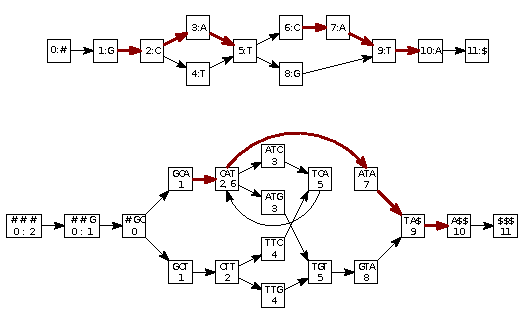
\includegraphics[width=0.8\textwidth]{Chapter2/Figs/sequence_graph_to_DBG.pdf}
  \caption[A sequence graph and its de Bruijn transformation]{
    \DIFaddFL{A sequence graph (top) and its de Bruijn transformation (bottom) for $k=3$.
    The highlighted path in the DBG is a false positive, as it consists of two disjoint paths in the input graph, and is shown to demonstrate the fact that the DBG is not a lossless representation of the input for any length greater than $k$.
    Reprinted from \mbox{%DIFAUXCMD
\cite{siren2017indexing}}\hspace{0pt}%DIFAUXCMD
.
  }}
  \label{fig:seq_graph_to_dbg}
\end{figure}

\DIFadd{To construct the GCSA2 index from variation graph $G$, we transform it into a de Bruijn graph whose nodes are the full set of $k$-length walks through the $G$ (as in figure \ref{fig:seq_graph_to_dbg}) on both strands.
Before doing so, to ensure that all elements }\DIFaddend of the graph \DIFdelbegin \DIFdel{.
Its external memory construction algorithm uses a prefix doubling approach to transform an input DBG of order }\DIFdelend \DIFaddbegin \DIFadd{are included in }\DIFaddend $k$\DIFdelbegin \DIFdel{to a pruned one of order $2^mk$ through $m$ doublingsteps.
The high-order DBGneed never be loaded into RAM but is induced from a lower-order DBG augmented with sufficient positional context on its nodes to support the disk-backed prefix doubling process.
In order to further reduce the complexity of the final index, the DBG input to GCSA2 may be constructed from a VG in which complex regions have been masked or reduced in local complexity using prior information such as a haplotype panel.
By default, }%DIFDELCMD < {\tt %%%
\DIFdel{vg}%DIFDELCMD < } %%%
\DIFdel{runs }\DIFdelend \DIFaddbegin \DIFadd{-length paths, we add head and tail nodes labeled $\#$ and $\$$ to the variation graph prior to this transformation.
To maintain the lexicographic ordering invariance required for searching in the }\DIFaddend GCSA2\DIFdelbegin \DIFdel{with initial }\DIFdelend \DIFaddbegin \DIFadd{, we add a special edge connecting these nodes prior to generating our $k$-mer set.}\footnote{\DIFadd{This can be seen in the LF mapping drawn between $BWT$ and $OUT$ in figure \ref{fig:gcsa2_search}, where a line connects $\$$ with $\#$.}}
\DIFadd{To allow larger query lengths without direct in-memory enumeration of the full length paths in the source variation graph, GCSA2 uses a series of disk backed steps to double the DBG $k$ until it reaches the desired length.
In practice, it uses four rounds of doubling, beginning with }\DIFaddend $k=16$\DIFaddbegin \DIFadd{, and progressing through $2k$, $4k$, $8k$, and $16k = 256$.
At each step, the DBG is pruned to remove redundancy and reduce memory usage (compare the graph in figure \ref{fig:gcsa2_search} to the DBG in \ref{fig:seq_graph_to_dbg}).
The final FM-index-like model is encoded using succinct data structures from }\href{https://github.com/simongog/sdsl-lite}{SDSL-lite} \DIFadd{\mbox{%DIFAUXCMD
\cite{gbmp2014sea}}\hspace{0pt}%DIFAUXCMD
, with succinct bitvectors used for rare characters like ${\tt N}$, $\$$, and $\#$.
}

\DIFadd{The final GCSA2 data structure model (illustrated in figure \ref{fig:gcsa2_search}) consists of: the $BWT$, which (as in SDBG) represents the edge space of the pruned DBG; $IN$, which marks which edge is the last among the inbound edges to a given node; $OUT$, which marks which edge is the last among the outgoing edges from a given node; and positional samples connecting the DBG nodes with positions in the input graph $G$.
As in the SDBG and GCSA, the nodes of the pruned DBG are not stored, but given implicitly in the number of 1-marked bits in $IN$ }\DIFaddend and \DIFdelbegin \DIFdel{$m=4$, yielding a final DBG with $k=256$.
Because it is based on a DBG}\DIFdelend \DIFaddbegin \DIFadd{$OUT$.
This can be seen in the relationship between the ``key'' vectors in figure \ref{fig:gcsa2_search} and the $BWT$ vector.
A vector (not shown in figure \ref{fig:gcsa2_search}) $C$ records the lexicographic ranges of the starting characters in the node labels, serving the same purpose as the equivalent vector in the FM-index.
For the index to be useful for graph path queries, we should be able to link lexicographic ranges within the BWT to positions in the original graph.
To do so, we store a set of positional samples as: a vector $B_S$, which indicates those nodes for which we have positional samples; a unary encoding of the number of values stored for each node $B_V$; and the vector of positional samples themselves $V_S$.
Positional samples are stored at the case of branches in the pruned DBG, or at some configurable frequency otherwise.
In linear regions of the pruned DBG, it is possible to use graph DBG graph traversal operations to compute un-sampled positions, thus trading off time and space as is typically done in FM-index implementations on linear strings.
}

\DIFadd{The GCSA2 encoding is highly efficienct on real data sets.
When including the suffix tree extensions}\DIFaddend , GCSA2 \DIFdelbegin \DIFdel{limits the maximum length query for which no false-positive results will be returned to the order }\DIFdelend \DIFaddbegin \DIFadd{uses around 1 bit per }\DIFaddend $k$\DIFdelbegin \DIFdel{of the DBG.
}%DIFDELCMD < 

%DIFDELCMD < %%%
\DIFdelend \DIFaddbegin \DIFadd{-mer in indexes of the 1000GP pangenome graph for $k=128$, which is favorable with comparison to SDBG indexes \mbox{%DIFAUXCMD
\cite{siren2017indexing}}\hspace{0pt}%DIFAUXCMD
.
}\DIFaddend To appreciate the costs of indexing a human genome sized graph\footnote{Precise sizes are given later in the discussion of results.}, the order-256 GCSA2 index of the 1000GP variation graph may be constructed using less than 500GB of scratch space, to and from which are written approximately 3TB during construction, all while requiring less than 50GB of RAM.
This puts GCSA2's indexing resource requirements well within the specifications of standard commodity compute servers.
The resulting index occupies between five and ten times the input graph's serialized size, no more than 50GB for a human genome.
\DIFaddbegin \DIFadd{Although it could appear to be a critical limitation, the limit on query length is not a problem in practice.
Few contemporary reads are likely to generate 256bp-long sequences with no mismatch from the reference}\footnote{\DIFadd{Illumina's reads rarely reach 256bp, and when they do they tend to have higher error rates in the later cycles. The 10-15\% error rate of PacBio and ONT sequencing mean that a 256bp exact match is extremely unlikely, although PacBio circular consensus reads (CCR) may approach this level of accuracy.}}\DIFadd{, this approach effectively allows us to find all the exact matches for a typical sequencing read.
}




%DIF > To be more precise, we find supermaximal exact matches (SMEMs) as defined in \cite{li2013aligning}.
%DIF > The addition of the longest common prefix (LCP) array alongside GCSA2's BWT effectively generalizes all essential operations on a suffix tree to the GCSA2, and enables us to find SMEMs and develop sensitive MEM-based seeding heuristics using the index.



%DIF > As an FM-index like structure, GCSA2 supports queries for a pattern $X$ that yield the suffix array interval matching a given pattern: $find(X) = ( sp_{X}, ep_{X} )$, and $locate( sp_{X}, ep_{X} ) = \{ b_1 \ldots b_{count(sp_{X}, ep_{X})} \}$ which yields the positions in the input VG where the given patterns occur.
%DIF > The LCP array allows the index to support several operations that require a suffix tree, including $count(sp_i, ep_i)$, which returns the number of matches for a given suffix array range, and $parent(sp_i, ep_i) = (sp_j, ep_j)$, which allows us to traverse the suffix links embedded in the suffix tree and forms the basis of maximal exact match (MEM) inference using GCSA2.

\begin{figure}[htbp!]
  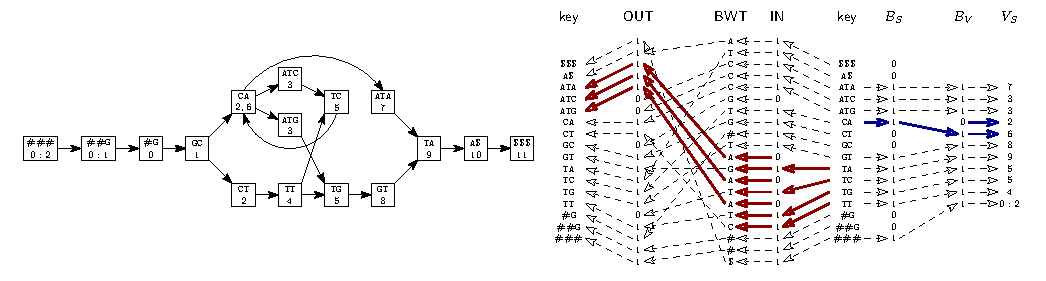
\includegraphics[width=\textwidth]{Chapter2/Figs/DBG_to_GCSA.pdf}
  \caption[Searching in the {\tt GCSA2}]{
    \DIFaddFL{Top: An order-3 pruned de Bruijn graph 3-equivalent to the de Bruijn graph in figure \ref{fig:seq_graph_to_dbg}.
    Bottom: the GCSA2 for the given graph, including both stored elements ($IN$, $OUT$, $BWT$, $B_S$, $B_V$, and $V_S$) and the implicit node sequences shown as the vectors labeled ``key''.
    Not shown, a vector $C$ encodes the number of nodes lexicographically smaller than a given character, supporting backward search and LF-mapping as in the normal FM-index.
    Leftward red arrows illustrate backward searching, showing the steps taken from }{\tt \DIFaddFL{T}} \DIFaddFL{to }{\tt \DIFaddFL{AT}}\DIFaddFL{.
    As in algorithm \ref{alg:bwt_find}, the range of nodes beginning with }{\tt \DIFaddFL{T}} \DIFaddFL{is found from two queries on $C$: $[sp, ep] = [C[T], C[T+1]-1] = [9,12]$.
    The lexicographic range in $BWT$ corresponding to this interval is found by $[select_{IN}(1, sp-1)+1, select_{IN}(1, ep)] = [10,16]$.
    We then apply LF-mapping (as in algorithm \ref{alg:bwt_find}) to find the range in $OUT$ corresponding to the pattern }{\tt \DIFaddFL{AT}}\DIFaddFL{.
    Finally, rank queries on $OUT$ allow us to convert to a lexicographic range of nodes prefixed by the pattern }{\tt \DIFaddFL{AT}}\DIFaddFL{, although in this case the mapping is trivial: $[sp,ep] = [rank_{OUT}(1,2),rank_{OUT}(1,4)] = [2,4]$.
    Rightward blue arrows mark the samples belonging to each node, with the blue ones showing them for node }{\tt \DIFaddFL{CAT}}\DIFaddFL{, which does not correspond to the given backward searching steps, but which would be found by another round of backward searching on }{\tt \DIFaddFL{C}}\DIFaddFL{.
    Reprinted from \mbox{%DIFAUXCMD
\cite{siren2017indexing}}\hspace{0pt}%DIFAUXCMD
.
  }}
  \label{fig:gcsa2_search}
\end{figure}

%DIF > GCSA2 resolves a number of problems that limit the utility of other graph path indexing schemes.
%DIF > Indexing a pruned DBG allows GCSA2 to be applied to arbitrary bidirectional string graphs that include reversals and loops.
\DIFaddend 

\subsection{Haplotype indexes}
%*1.5p 3h*
% worth mentioning gpBWT and PBWT
Recording the path set of a graph in XG (described in section \ref{sec:graph_topology_index}) requires $O(N\overline{P} + {\cal L}|P|)$ space where ${\cal L}$ is the average haplotype length in terms of nodes it crosses, $N$ is the number of nodes in the graph, $|P|$ is the number of paths in the graph, and $\overline{P}$ the average number of paths crossing each node.
Although, such a representation can be compressed, the size of this representation will grow linearly with the addition of new paths, making it impractical as a means to record very large numbers of genomes.

Recording collections of paths is an important requirement for the use of VG in resequencing, as the Markovian property of the bare sequence graph $G = (N, E, P= \emptyset)$ means it can encode exponentially many paths relative to the true input path set used to build the graph.
This introduces significant issues during read mapping and genome inference.
With increasing variant density the number of possible sequence paths of a given length grows exponentially, and this can lead to spurious mismapping (section \ref{sec:1000GP_sim}).
The exponential growth of the path space of the graph has relevance for sequence indexing with GCSA2, and as described in \ref{sec:graph_sequence_indexes}, simplification of the graph in complex regions prior to GCSA2 indexing is required to build indexes in practice.
A haplotype index allows the pruning operation to preserve known haplotypes, rather than defaulting to the reference genome in such cases.
Efficient path indexes could be used for many operations in variant calling and phasing, and may have utility in assembly problems, for instance to losslessly record a read set embedded in a \DIFdelbegin \DIFdel{squish }\DIFdelend \DIFaddbegin \DIFadd{variation }\DIFaddend graph representing their mutual alignment (section \ref{sec:from_pairwise_alignments}).

Haplotype sequences from the genomes of the same species often share extensive regions \DIFaddbegin \DIFadd{of homology}\DIFaddend , which suggests that they may be very efficiently compressed.
This property was used to store large haplotype sets in the \emph{positional BWT} (PBWT) \cite{durbin2014efficient}.
As input, the PBWT assumes a set of haplotype strings $S_1 \ldots S_m$ of the same length which describe a set of haplotypes relative to a set of variable loci.
$S_j[i]$ records the allele in haplotype $j$ found at locus $i$.
We set $S_j[i] = 0$ when haplotype $j$ has the reference allele at locus $i$, and $S_j[i] > 0$ if it encodes one of possibly several alternate alleles.
The PBWT can be understood as an FM-index of texts $T_1 \ldots T_m : T_j[i] = (i, S_j[i])$ \cite{gagie2017wheeler}.
To search for a haplotype of $h$ in the range $[i,j]$ we look for pattern $h' = (i, h[1]) \ldots (j, h[|h|])$.
The alphabet size of this FM-index is large, but the matrix like structure of the haplotype set means that we can implicitly encode the array indexes by building a separate sub index for each position.
Applying run length encoding to the BWT allows extremely good compression of real haplotype sets.

With the \emph{graph positional Burrows–Wheeler transform} (gPBWT) \cite{Novak2017gPBWT}, we extended this model to work on variation graphs.
The basic model is the same as the generic PBWT except that instead of variant matrix positions we consider haplotype traversals of oriented nodes\footnote{These are described as ``sides'' in \cite{Novak2017gPBWT}.} $n_i$ or $\overline{n_i}$, and rather than a local alphabet of variant alleles we encode a local alphabet $\Sigma_{n_i} = \{ j \in N | e_{ij} \in E \}$ which describes the set of nodes $n_{\{j \in N | e_{ij} \in E \}}$ to which haplotypes \DIFdelbegin \DIFdel{go }\DIFdelend \DIFaddbegin \DIFadd{continue immediately }\DIFaddend after the current node $n_i$.
As in the generic PBWT we build an FM-index of $T_1 \ldots T_m$, encoded in what we call the $B_s$ arrays, which provide the local description of prefix sorted haplotypes (equivalently, threads) traversing each node $n_s$.
To deal with the bidirectionality of paths in variation graphs, each haplotype must be encoded in its forward and reverse orientation.
In \cite{Novak2017gPBWT} we demonstrated the expected sublinear scaling of the gPBWT by building an index for chr22 with increasing numbers of samples.
Constructing the gPBWT for haplotype sets representing more than a few hundred samples proved difficult when using our particular implementation.
Progressive construction of the gPBWT in generic graphs was enabled by encoding the gPBWT into dynamic succinct data structures and adding a single haplotype thread and its inverse one at a time.
While functional, we found this to be untenable for large graphs and haplotype sets.
Overheads associated with the dynamic data structures it uses were significant, but the most-difficult issue was the serial nature of the progressive construction algorithm, which gives the algorithm $O(m)$ runtime.
Consequently, all our large-scale experiments were carried out using a partially ordered construction algorithm that worked using a VCF file as input.


\DIFaddbegin \begin{figure}[htbp!]
  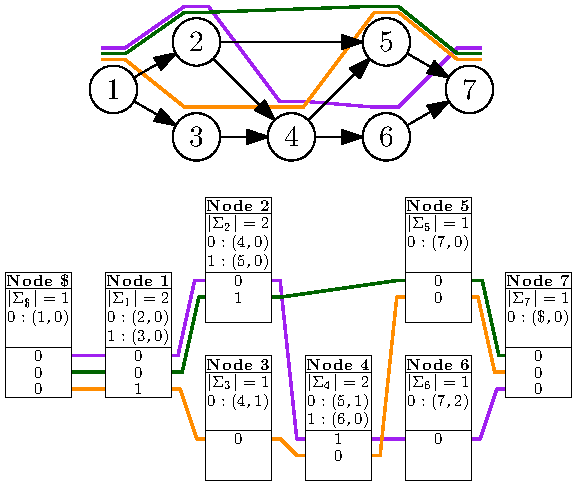
\includegraphics[width=\textwidth]{Chapter2/Figs/gbwt-example.pdf}
  \caption[The Graph Burrows Wheeler Transform]{
    \DIFaddFL{Top: A graph with three paths, each represented as a colored line walking above a series of nodes, where $N={n_1\ldots n_7}$.
    Bottom: GBWT of the paths.
    To build the GBWT we first append a marker node, $n_\DOLLAR $, to the head of the graph.
    Each node in the GBWT is represented by a record, shown as a white box.
    At the top of each record we find the node identifier, which is implicitly stored in the actual GBWT.
    Each record consists of a local alphabet described in a header and a body consisting of the subset of the full GBWT applying to the given node.
    The alphabet $\Sigma_i$ maps nodes which paths crossing this node reach in their next step into a more compact alphabet.
    It is encoded as a mapping between next node identifier $i$, the local character used to represent that node $\in [0 \ldots |\Sigma_i|)$, and the number of instances of $i$ in the BWTs of all nodes which are lexicographically smaller than the current one.
    For instance, at $n_6$ we find $\Sigma_6 = \{ 0: (7, 2) \}$, because $n_7$ is referred to by the orange and green path crossing the edge $n_5 \to n_7$.
    This arrangement encodes the full BWT in per-node local records.
    We see each path represented as it passes through the BWT record for each node.
    At each node, the sort order of the paths implicitly represented in the BWT reflects the lexicographic sort of their prefixes.
    For instance, at $n_4$, we see $n_{BWT} = [1, 0]$, because the prefix of the purple path before $n_4$ is encoded as $[0,0,0]$, which is lexicographically lower than the prefix of the orange path, $[0,1,0]$.
    Reprinted from \mbox{%DIFAUXCMD
\cite{siren2018haplotype}}\hspace{0pt}%DIFAUXCMD
.
  }}
  \label{fig:gbwt-example}
\end{figure}

\DIFaddend The \emph{graph Burrows-Wheeler transform} (GBWT) \cite{siren2018haplotype} simplifies the data model used by gPBWT so that it is independent of {\tt vg}.
\DIFdelbegin \DIFdel{The }\DIFdelend \DIFaddbegin \DIFadd{Conceptually, the }\DIFaddend GBWT can be understood as the FM-index of a transformation of the graph's paths $p_1\ldots p_m \cup \overline{p_1}\ldots \overline{p_m}$ into the text $T = \$( p1 = n_i\ldots n_j) \ldots \$ (\overline{p_m} = \overline{n_j} \ldots \overline{n_i}) $ wherein the paths are rewritten as a series of characters representing node traversals in a large alphabet and delimited by a marker $\$$.
This approach is challenging due to the large size of $T$ for moderately-sized haplotype sets embedded in variation graphs, e.g. $|T| \approx 10^{12}$ for the 1000GP \cite{siren2018haplotype}.
\DIFaddbegin \DIFadd{Literally implementing this model would require a large alphabet CSA with suboptimal performance bounds.
}\DIFaddend Serializing the path set during construction is not feasible, which suggests a dynamic version of the model is required \DIFaddbegin \DIFadd{during large scale construction.
Natural variation graphs have a number of properties, such as a manifold partial order, which ca be exploited to improve the memory usage of the GBWT}\DIFaddend .

In the GBWT we break the full FM-index into per-node records, each of which encodes a header defining an alphabet $\Sigma_{n_i}$ of all the nodes that follow $n_i$ in any path, and a body $BWT_{n_i}$ which is the subset of the full BWT specifying which node follows $n_i$ in each path that passes through $n_i$, with the paths sorted in reverse sequence order up until $n_i$.
Since paths that are similar before $n_i$ tend to be similar after it, this sequence of next node values run length compresses well.

The GBWT supports essential FM-index operations including: $find(X) \to [sp, ep]$ yielding the lexicographic range of suffixes starting with pattern $X$; $locate(sp, ep) \to$ paths occurring in $SA[sp, ep]$; and $extract(j) \to p_j$ which returns the $j$th path in the graph.
By encoding all paths in both orientations, the GBWT can be treated as a kind of FMD-index for haplotypes, allowing bidirectional search.
This means that the GBWT in turn supports MEM-based haplotype matching, which has potential uses in genotype imputation, phasing, association mapping, and other population genetic and evolutionary assays.
\DIFaddbegin \DIFadd{Although supported, this particular modality has not yet been explored.
}\DIFaddend 

The GBWT representation reflects a number of assumptions that tend to hold for most DNA sequence graphs.
Nodes tend to have low degree, which means the local alphabet size $|\Sigma_{n_i}|$ is small, and we can afford to decompress a small local alphabet encoding efficiently.
Most nodes are not traversed more than once by each path, so the $BWT_{n_i}$ remains small and can be accessed and modified in bounded time.
Due to relatedness among individuals in many species, it is sensible to assume that haplotypes will be highly repetitive, which allows for efficient RLE encoding of $BWT_{n_i}$.
The graph is sorted, and its identifier space has been compacted, which allows us to store the same information for the entire range of node identifiers in bounded memory with respect to $|N|$.
The graph tends to be locally ordered in most places, which decreases the complexity of construction.

\DIFdelbegin %DIFDELCMD < \begin{figure}[htbp!]
%DIFDELCMD <   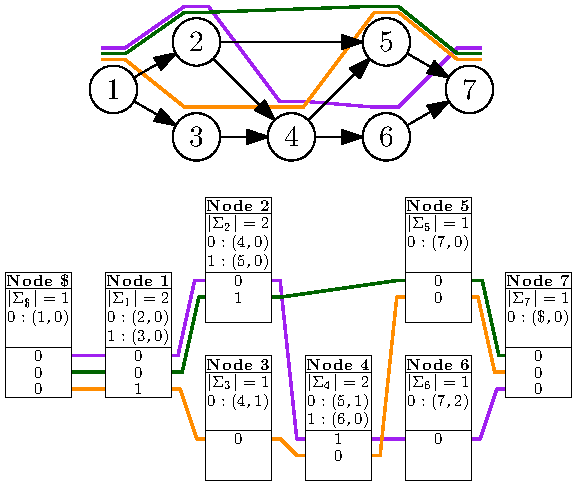
\includegraphics[width=\textwidth]{Chapter2/Figs/gbwt-example.pdf}
%DIFDELCMD <   %%%
%DIFDELCMD < \caption[The Graph Burrows Wheeler Transform]{%
{%DIFAUXCMD
\DIFdelFL{Left: A graph with three paths. Right: GBWT of the paths.
    Reprinted from \mbox{%DIFAUXCMD
\cite{siren2018haplotype}}\hspace{0pt}%DIFAUXCMD
.
  }}
  %DIFAUXCMD
%DIFDELCMD < \label{fig:gbwt-example}
%DIFDELCMD < \end{figure}
%DIFDELCMD < 

%DIFDELCMD < %%%
\DIFdelend A \emph{dynamic GBWT} implementation presents the node records through an index over the range of $[min(i : n_i \in N), max(i : n_i \in N)]$, for each linking to its header, body, incoming edges, and haplotype identifiers.
Construction employs this model in a manner similar to RopeBWT2 \cite{li2014fast}, where batches of paths are insert into the index in a single step following the BCR construction algorithm \cite{bauer2013lightweight}.
This process includes the new paths in the dynamic GBWT by rebuilding each node record affected by the extension.
\DIFdelbegin \DIFdel{When constructed, the GBWT may be encoded in a compacted but immutable form that uses less memory.
}\DIFdelend By breaking the construction process apart for each chromosome and finally merging the compressed GBWTs, it is possible to build the GBWT for the entire 1000GP haplotype set in around 30 hours.
\DIFaddbegin \DIFadd{When constructed, the GBWT may be encoded in a compacted but immutable form that uses less memory by representing the per-node model of the dynamic GBWT in a columnar model, for instance concatenating the node BWT vectors and header information for each node each into a single compressed integer vector.
}\DIFaddend The resulting GBWT requires $\approx 15$ GB, with around half allocated to the GBWT structure itself and half to haplotype identifiers.
The index consumes less than 0.1 bit per node in the stored paths, and we should expect this to improve when we build the GBWT for larger haplotype panels.

\subsection{Generic disk backed indexes}
%*0.5p 0.5h*
\label{sec:generic_disk_backed_indexes}
I began the development of {\tt vg} alone, starting with schemas for the data models, then building an index of the graph using the disk-backed key/value store RocksDB\footnote{\url{https://github.com/vgteam/vg/blob/master/src/index.hpp}}.
I transcribed the data model into namespaces and sorted arrays written into the key/value store.
As compressors of various types could be applied to the sorted arrays backing RocksDB, the memory required for this approach was ultimately similar to that for the final indexing models that I present here.
However, performance was far worse, and the initial version of the aligner based on these systems could not achieve correct results using reasonable amounts of time for large graphs.
Ultimately, this flexible database model has remained important for some pipelines, in particular as a technique to organize alignments against the graph.
Other workloads such as sequence queries were untenable for large genomes, with reliable performance only possible if the entire index of spaced $27$-mers was cached in RAM, requiring nearly 200G in the case of the 1000GP variation graph.
The sorted disk-backed array does have the useful property of allowing prefix queries of the $k$-mer set, but this can easily be attained with GCSA2.
On the networked storage available in my institutional setting, the construction costs for disk-backed index models were usually much worse than those of the XG and GCSA2 models.

\subsection{Coverage index}
\label{sec:coverage_index}

A coverage map, of the alignments to a VG is similar to the labeling required to implement ``colors'' on a DBG \cite{iqbal2012}.
The coverage map loses information about the edge traversals and the paths taken through the graph, which could reduce the visibility of some kinds of variation within it.
But in benefit, this simple model is efficient to use.
The complexity of computing the coverage map is linear in the number of \DIFdelbegin \DIFdel{the input alignment set}\DIFdelend \DIFaddbegin \DIFadd{input alignments}\DIFaddend , and it requires $O(\sum_{\forall{n_i\in N}}|n_i|)$ space to store once built.

I developed an compact coverage index by mapping the sequence space of the graph into a vector and recording coverage across it for a GAM read set.
During construction, a succinct format is employed to store each base's coverage in a single byte as long as it is below 255, and in a secondary hash table if it reaches or exceeds 255.
Finally, a compressed integer vector is generated, which can be queried by graph position computed from the XG index of the graph.
I extended this concept with a succinct ``pileup'' format \cite{li2009sequence} generated from the edits against the graph.
In this model edits in mappings which don't match the reference were serialized into a byte alphabet using Protobuf, such that each non-reference edit $e_j$ at position $b_i$ was recorded as a string $\$b_i e_j$, with the idea that by building a CSA/FM-index from these I could obtain the set of edits at each graph position through pattern matching.
However, I found it impossible to construct this for a large high-coverage sequencing sample, and have not continued this line of investigation.

\section{Sequence alignment to the graph}
%*0.5p 0.5h*
To align sequences to a VG, we use the graph and sequences indexes described in the previous section (\ref{sec:index_structures}) to derive MEMs between a query and the graph.
A \DIFdelbegin \DIFdel{Markovian }\DIFdelend \DIFaddbegin \DIFadd{weighted DAG collinear }\DIFaddend chaining model is built from the MEMs which respects their relative positions in the graph and the read, favoring collinear mappings of MEMs, and \DIFdelbegin \DIFdel{Viterbi is used }\DIFdelend \DIFaddbegin \DIFadd{a max-sum DP algorithm is applied to this alignment DAG }\DIFaddend to extract likely mappings based on the MEMs.
We then align the sequence locally to the graph at each of the high scoring chains using various sensitive alignment algorithms that use various kinds of dynamic programming.

To detect structural variation and align long reads without incurring quadratically-scaling computational penalties, we apply a kind of banding and a second layer of chaining.
In \emph{chunked alignment}, large sequences are broken up into overlapping segments, each of which is aligned individually in any order or orientation.
This subdivision provides a kind of banding to the alignment algorithm, preventing the evaluation of the full DP matrix, but more importantly it also allows alignments that are generated to represent any kind of variation.
Each chunk is aligned independently.
The same collinear chaining model, with different parameters, is used to establish the optimal global chain through the alignment chunks, thus yielding a full alignment for an input sequence of any size.
Where our reads are shorter than the standard chunk size (256bp), the alignment behaves exactly as in {\tt bwa mem}.
Figure \ref{fig:alignment_to_cactus_yeast} illustrates the alignment of a long read against a complex graph.

\emph{Unfolding} and \emph{DAGification} transform a cyclic bidirectional sequence graph with inversions to an acyclic simple sequence graph one in which all $k$-paths in the first graph are represented.
Any alignment algorithm that may be implemented on a sequence DAG can thus be used.
Optionally, other alternative DP alignment algorithms implementing a banded global alignment can be applied, and I describe one of these that I implemented to \emph{surject} alignments into a particular reference path.

\begin{figure}[htbp!]
\centering
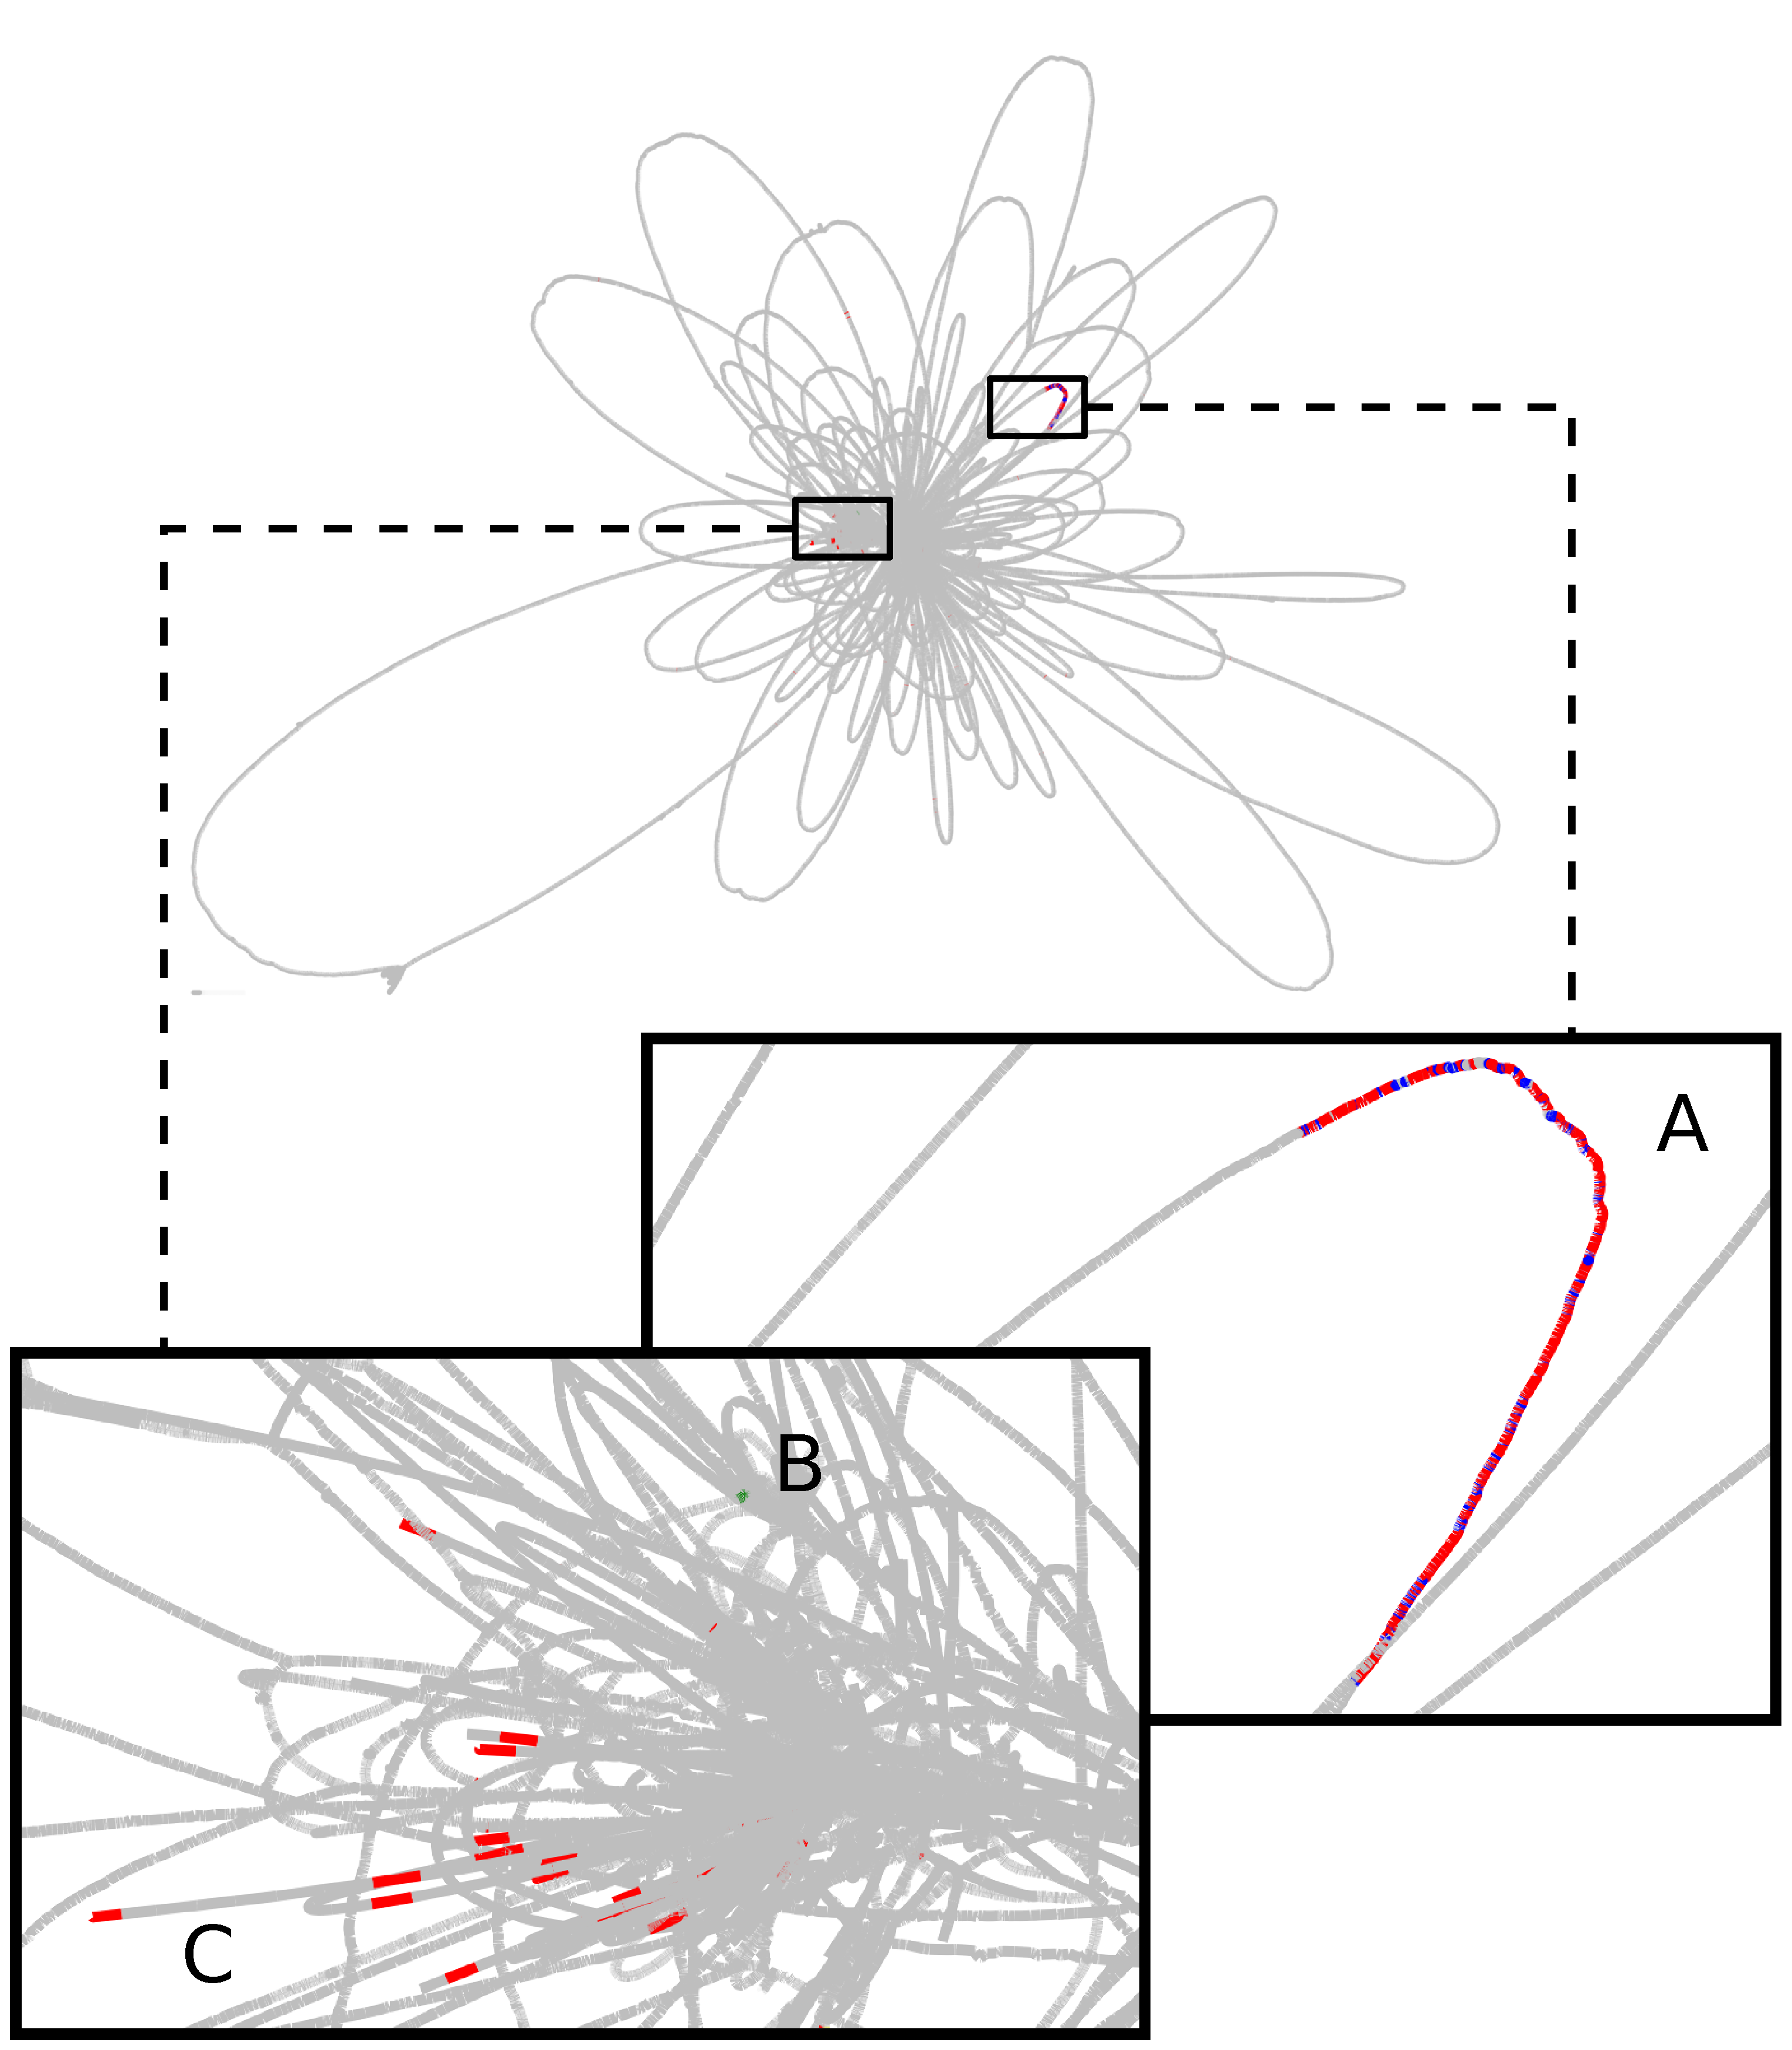
\includegraphics[width=1.0\textwidth]{Chapter2/Figs/mapping_cactus_pacbio_aln_vizzy.pdf}
\caption[Alignment of a PacBio read to a yeast pangenome]{
  Aligning a 32,737bp PacBio read from the SK1 strain to a yeast pangenome graph (section \ref{sec:yeast_cactus}).
  Red nodes contain initial MEM hits, while other nodes are colored if they were matched during local alignment.
  (A) The nodes found in the best alignment are labeled in blue.
  (B) A much smaller secondary alignment is shown in green.
  (C) MEM hits for this read cluster in chromosome ends, which are seen as tips in the graph visualization.
}
\label{fig:alignment_to_cactus_yeast}
\end{figure}


\DIFaddbegin \begin{figure}[htbp!]
\centering
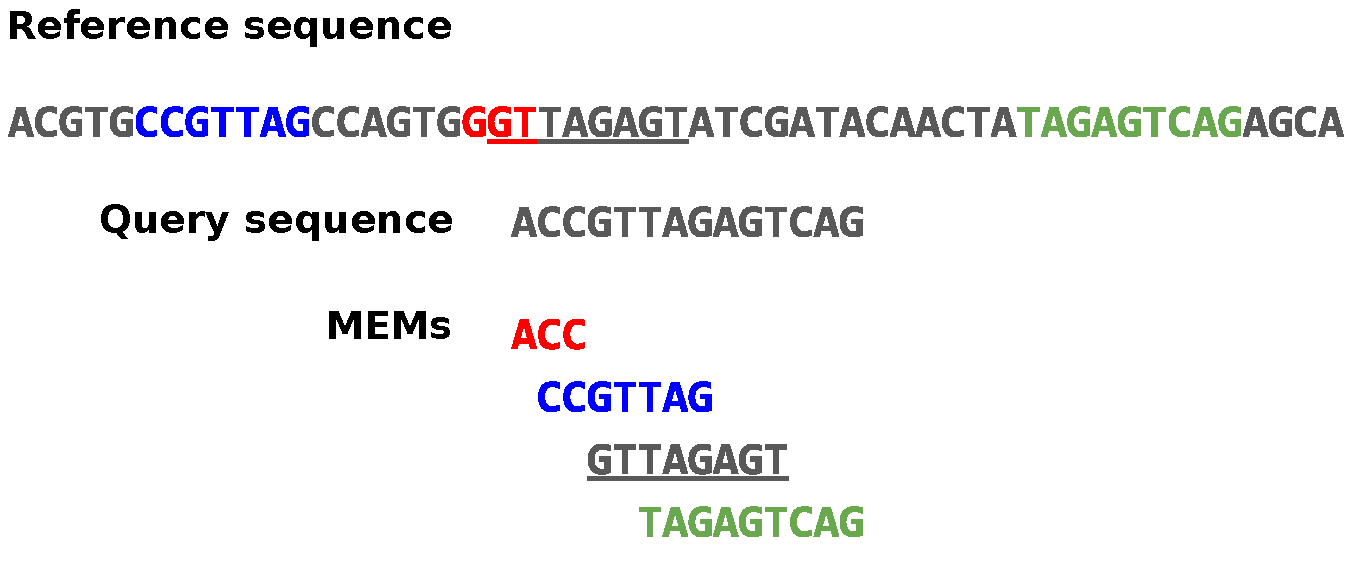
\includegraphics[width=0.8\textwidth]{Chapter2/Figs/mem-finding.pdf}
\caption[Finding maximal exact matches (MEMs)]{
  \DIFaddFL{Maximal exact matches (MEMs) found by the application of algorithm \ref{alg:mem_find} to the given query sequence and a GCSA2 index built from the shown reference sequence.
  MEMs are listed below the query sequence with colors that match their matching location in the reference sequence.
  Note that one MEM is found on the reverse strand of the reference (}{\tt \DIFaddFL{ACC}} \DIFaddFL{matches }{\tt \DIFaddFL{GTT}}\DIFaddFL{).  
}}
\label{fig:mem_finding}
\end{figure}


\DIFaddend \subsection{MEM finding \DIFaddbegin \DIFadd{and alignment seeding}\DIFaddend }
%*2p 2h*
\DIFdelbegin \DIFdel{First, a }\DIFdelend \DIFaddbegin \DIFadd{A }\DIFaddend set of super-maximal exact matches (SMEMs) of a query sequence are generated by \DIFdelbegin \DIFdel{traversing the suffix tree encoded }\DIFdelend \DIFaddbegin \DIFadd{backward search }\DIFaddend in the GCSA2 index\DIFdelbegin \DIFdel{until the count of matching strings drops to 0, then backing off one step to find all longest exact matches.
A recursive }\DIFdelend \DIFaddbegin \DIFadd{.
When backward search breaks, we step back to the last matching interval and use the suffix tree extension of the index to obtain the parent node of this interval.
The GCSA2's }{\tt \DIFadd{LCPArray}} \DIFadd{extension allows interrogation of the suffix tree structure, which in turn this allows us to remove the invariant sequence from the end of our previous matched range and continue search for the next maximal match.
Algorithm \ref{alg:mem_find} provides a sketch of this process as it relates to the GCSA2 FM-index encoding and LCPArray.
}

\DIFadd{Not shown in this algorithm sketch are a }\DIFaddend series of ``\DIFdelbegin \DIFdel{reseed'' passes through the traversal can then identify distinct next-longest matches which are used both to improve sensitivity .
These }\DIFdelend \DIFaddbegin \DIFadd{reseeding'' passes where by long MEMs are used as the basis for further exact match finding, but with a maximum limit to the detected match size.
When backward search yields an exact match of this size, we use the same suffix tree operation to reset our match range with the next possible match.
This reseeding operation is required to obtain high sensitivity via MEM based alignment seed lookup.
At sufficient frequency to frustrate our mapping sensitivity in real genomes, a long MEM can mask out shorter sub-matches that might be contained within it, and which correspond to the correct mapping location.
The resulting MEMs }\DIFaddend are not super-maximal, thus we tend to call these heuristically derived exact matches ``MEMs'' \DIFdelbegin \DIFdel{.
Then, chains }\DIFdelend \DIFaddbegin \DIFadd{for simplicity.
}

%DIF > the suffix tree encoded in the GCSA2 index until the count of matching strings drops to 0, then backing off one step to find all longest exact matches.
%DIF > A recursive series of ``reseed'' passes through the traversal can then identify distinct next-longest matches which are used both to improve sensitivity.

\DIFadd{We use MEMs to seed alignments in }{\tt \DIFadd{vg}}\DIFadd{.
As indicated in algorithm \ref{alg:mem_find}, the GCSA2 index supports lookup of matches by position in the original graph.
In conjunction with a distance estimator, these positions are used to build a collinear chaining model that allows us to estimate likely subgraphs matching our query (described subsequently in section \ref{sec:collinear_chaining}).
Chains }\DIFaddend of MEMs that are consistent with \DIFaddbegin \DIFadd{a mapping between }\DIFaddend the query sequence \DIFaddbegin \DIFadd{and the graph }\DIFaddend are found using a \DIFdelbegin \DIFdel{Markov }\DIFdelend \DIFaddbegin \DIFadd{weighted graphical }\DIFaddend model in which the optimal alignment is likely to form a \DIFdelbegin \DIFdel{Viterbi }\DIFdelend \DIFaddbegin \DIFadd{max-sum }\DIFaddend path.
For each candidate chain, we then locally align the read against the graph. 
Scoring results from the local alignment are used to rank the candidate alignments.
We then return the best alignment, or multiple candidates if multiple mappings are required\DIFaddbegin \DIFadd{, with calculation of mapping quality used to provide an estimate in our confidence in the best alignment (section \ref{sec:mapping_quality})}\DIFaddend .

\DIFaddbegin \begin{algorithm}
  \caption[MEM finding]{
    \DIFadd{Finding maximal exact matches using the GCSA2 suffix tree extension
  }}
  \label{alg:mem_find}
  \begin{algorithmic}
    \Function{FindMEMs}{Q} \Comment{Find the MEMs for the given query sequence $Q$}
    \State \DIFadd{$mems \gets \emptyset$ }\Comment{The list of MEMs that we'll return}
    \State \DIFadd{$c \gets Q[|Q|-1]$ }\Comment{Current character in our search}
    \State \DIFadd{$sp \gets C[c]$ }\Comment{Beginning of our SA interval}
    \State \DIFadd{$ep \gets C[c+1]-1$ }\Comment{End of our SA interval}
    \State \DIFadd{$mem.begin \gets |Q|-2$ }\Comment{Build up a MEM structure to store our current match}
    \State \DIFadd{$mem.end \gets |Q|-1$ }\Comment{Record the current matching interval}
      \For{$i \in [|Q|-2 \ldots 0]$} \Comment{Step backwards through the string}
        \State \DIFadd{$last = [sp, ep]$ }\Comment{Store the last range, in case search breaks}
        \State \DIFadd{$c \gets Q[i]$ }\Comment{Update our character}
        \State \DIFadd{$sp \gets C[c] + rank_{BWT}(c, sp - 1)$ }\Comment{Update $sp$ dependent on $c$}
        \State \DIFadd{$ep \gets C[c] + rank_{BWT}(c, ep) - 1$ }\Comment{Do the same for $ep$}
        \If{$sp > ep$} \Comment{The current extension has failed}
          \State \DIFadd{$mem.begin \gets i + 1$ }\Comment{Remove the last (unmatched) character}
          \State \DIFadd{$mem.range \gets last$ }\Comment{Set the range to the last matching range}
          \State \DIFadd{$mem.positions \gets GCSA2.locate(mem.range)$ }\Comment{Get MEM positions}
          \State \DIFadd{$mems.append(mem)$ }\Comment{Store the last MEM for return}
          \State \DIFadd{$p \gets LCP.parent(last)$ }\Comment{Get the suffix tree node parent of the last range}
          \State \DIFadd{$mem.end \gets mem.begin + p.lcp()$ }\Comment{Remove the common prefix}
          \State \DIFadd{$[sp, ep] \gets p.range()$ }\Comment{Use the SA range of the suffix tree parent node}
        \EndIf
        \EndFor
      \State \DIFadd{$mems.append(mem)$ }\Comment{Add the last MEM to the MEMs to return} \\
      \Return{$mems$} \Comment{Return the MEMs we've found}
    \EndFunction
  \end{algorithmic}
\end{algorithm}

\DIFaddend \subsection{Distance estimation}
\label{sec:distance_estimation}
%*1p 1h*
To cluster our MEMs we require a distance function that returns the minimum distance between any two positions $dist(b_i, b_j)$. % \to \min_{\forall p \in N \times N}{|p|} : pos(p[1]) = b_i \land pos(p[|p|]) = b_j$.
Distance measurement between nodes in a variation graph is non-trivial, with exact solutions to the problem theoretically requiring $O(E \log \log L)$ where $L = \max_{\forall n_i \in N} |n_i|$ is the maximum node length \cite{karlsson1983mlog}.
Precomputation of the full set of distances would thus require $O(N^2 E \log \log L)$ time and $O(N^2)$ space, which is infeasible for any large graph.
Many variation graphs are mostly linear, which we can exploit to build an approximate distance metric.
Provided we have applied a partial sort to the graph, in the partially ordered regions we can use the offset of each node in the XG sequence vector $S_\textbf{iv}$ as an approximate 1D coordinate, which we query using the corresponding rank/select dictionary $S_\textbf{bv}$.
We expect that in much of the graph $S_\textbf{bv}^{select_1}(id(b_j))+\mbox{offset}(b_j) - S_\textbf{bv}^{select_1}(id(b_i))+\mbox{offset}(b_i) \propto dist(b_i, b_j)$, where $id(b)$ is the function that returns the rank of position $b$'s node in the XG index, and $\mbox{offset}(b)$ returns the position's offset inside the sequence label of the node.

Nonlinearities in the graph will frustrate this metric, and to manage these we rely on the positional index provided by the \emph{positional paths} given in the XG index.
In these, we can query the relative positions of nodes in the path in $O(1)$ time.
Where both positions are not on the same path, we \DIFdelbegin \DIFdel{can use }\DIFdelend \DIFaddbegin \DIFadd{use a bounded }\DIFaddend local exploration of the graph near our positions $b_i$ and $b_j$ to attempt to find anchoring nodes on the same path.
In our clustering step \DIFdelbegin \DIFdel{we can }\DIFdelend \DIFaddbegin \DIFadd{(section \ref{sec:collinear_chaining}) we }\DIFaddend consider the multiple coordinate systems to develop a global pseudoalignment.

\subsection{Collinear chaining}
%*0.5p 0.5h*
\label{sec:collinear_chaining}

\DIFdelbegin \DIFdel{If the }\DIFdelend \DIFaddbegin \DIFadd{In most cases, single }\DIFaddend MEMs do not cover the full read length, \DIFdelbegin \DIFdel{then we attempt to link them together into chains by building a Markov model in which the best possible chains form high-scoring paths.
In this model the nodes correspond to the reference graph positionswhere MEMs in the read occur and the transitions between nodes correspond to a weight that is proportional to the indel size implied by the difference in }\DIFdelend \DIFaddbegin \DIFadd{so we need to combine information from multiple MEMs to determine a candidate mapping location.
It is impractical to attempt a full DP based alignment at each MEM location, and instead, we apply a heuristic approach wherein a model is built with the available MEM seed information, their graph positions, their positions in the query sequence, and the scoring parameters used for local alignment.
The }\emph{\DIFadd{MEM Chain Model}} \DIFadd{is a DAG, $G_\textsc{MemChain} = (N, E)$, in which each node $n_i \in N$ derives from a MEM, and each edge $e_{ij} \in E$ to represent a possible transition between MEMs that we may find in an alignment.
}

\begin{figure}[htbp!]
\centering
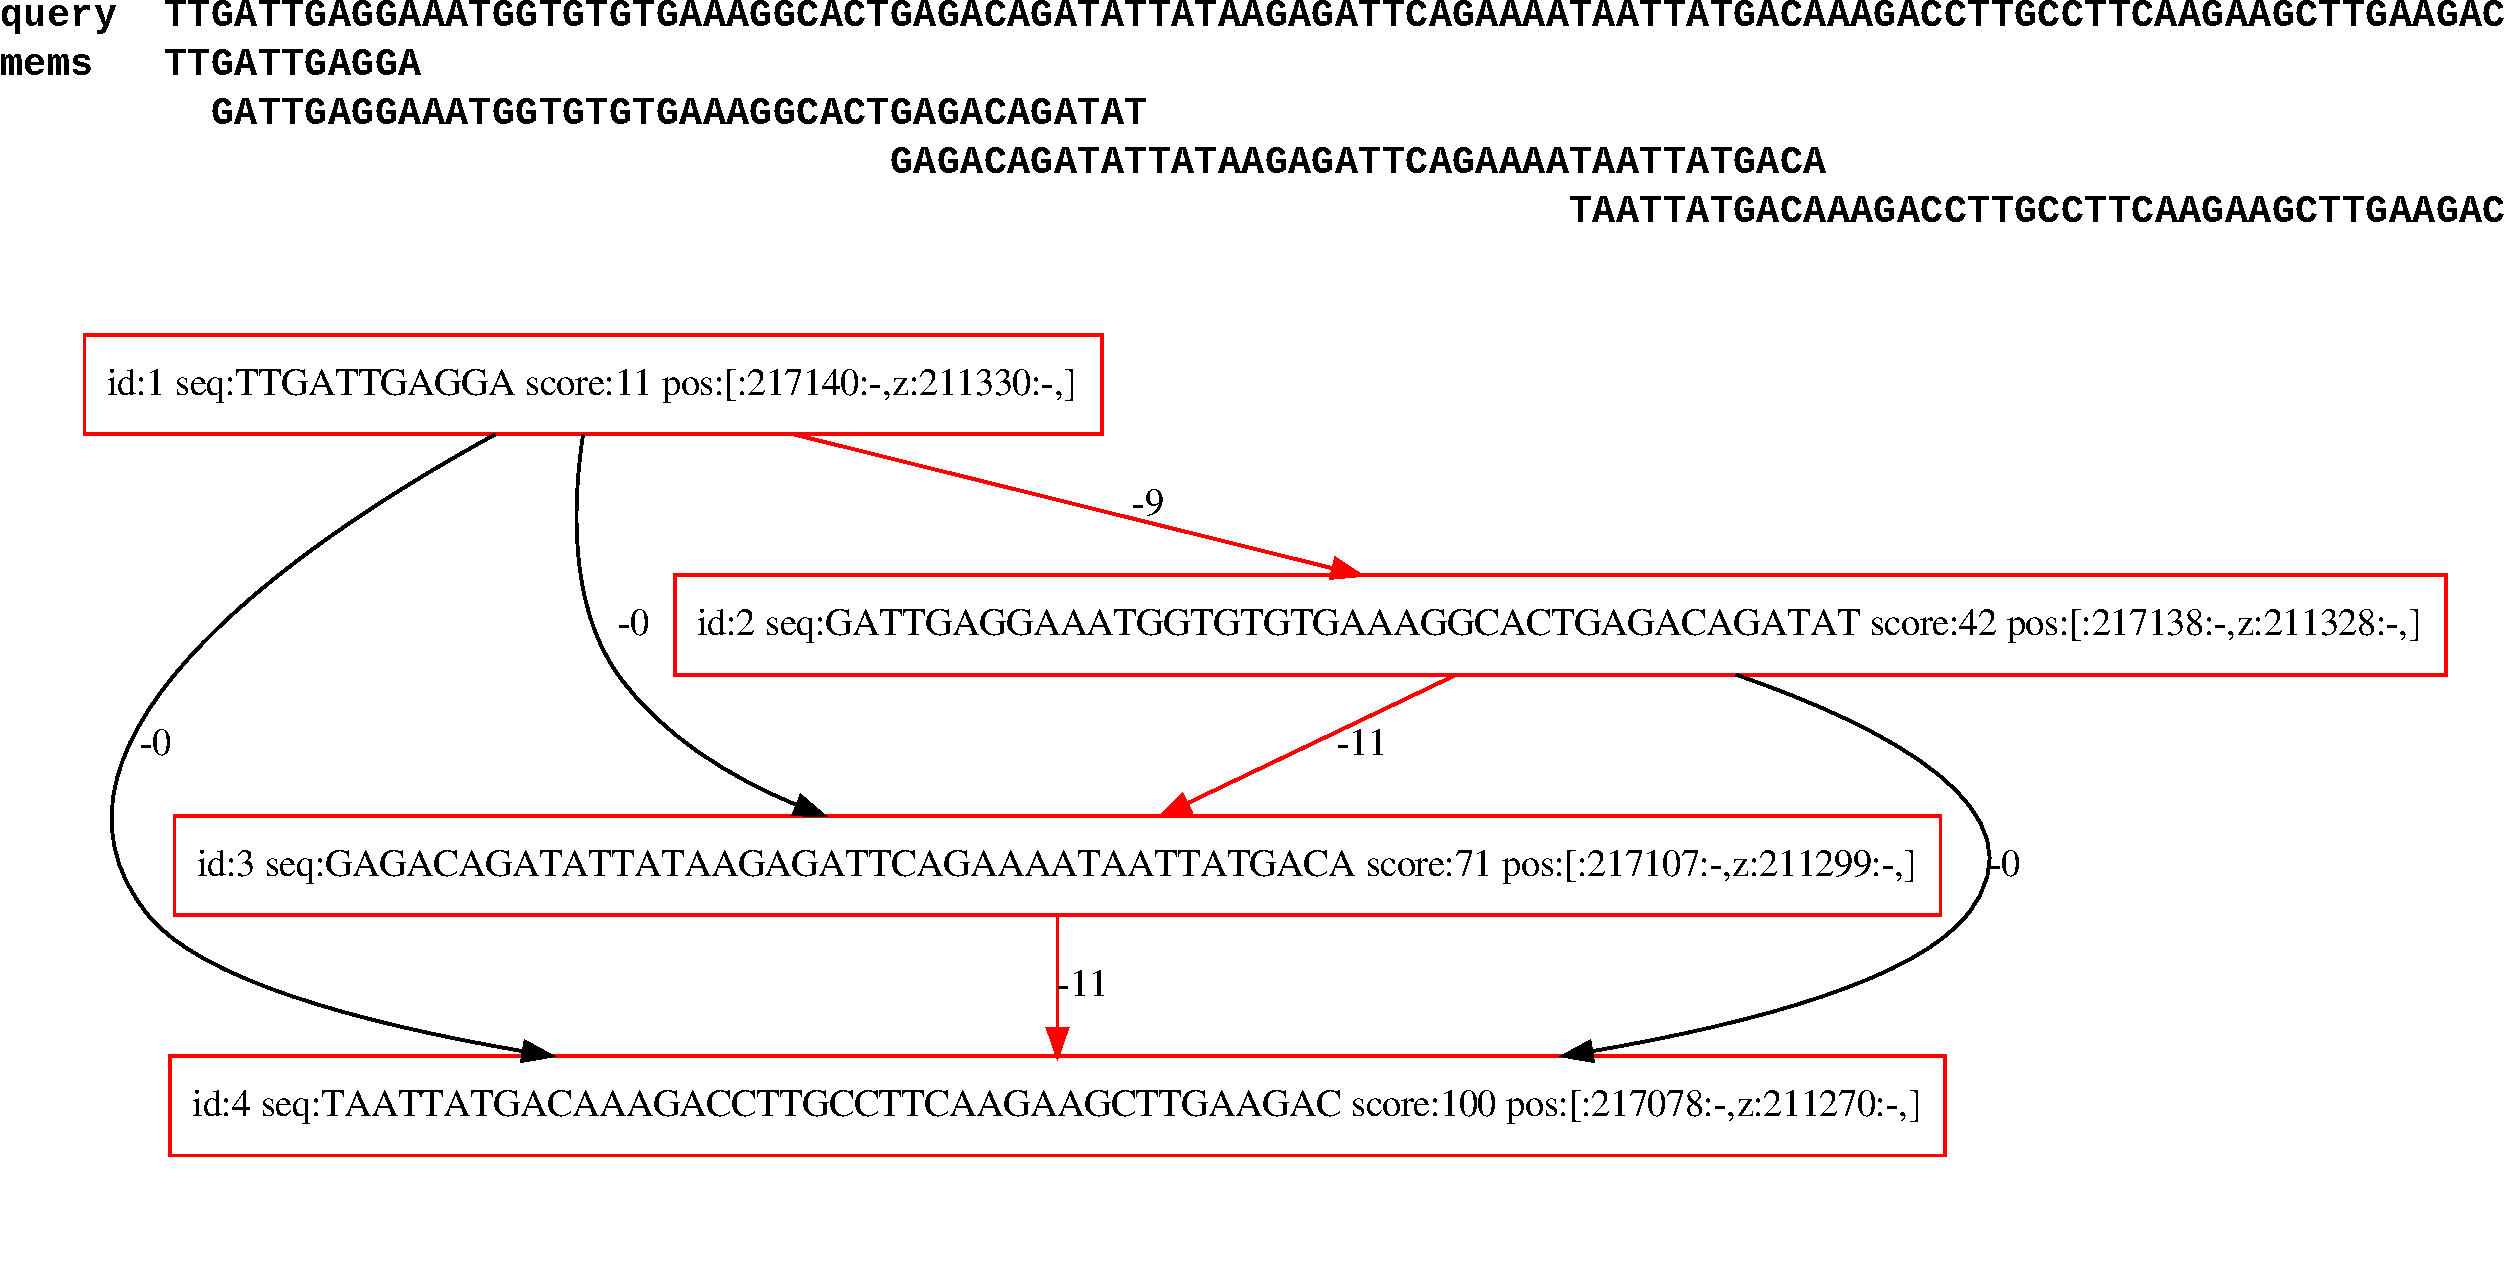
\includegraphics[width=1.0\textwidth]{Chapter2/Figs/memchain_dag.pdf}
\caption[The MEM Chain Model]{
  \DIFaddFL{Establishing collinear chains of MEMs to drive sequence read mapping.
  Above: a set of MEMs derived from a perfect read simulated from a 1 Mbp test region from the 1000GP graph of chr20, using a maximum MEM length of 40bp to generate multiple MEMs for exposition.
  Below: the first evaluation of the MEM Chain Model for this set of MEMs.
  The model is shown in full, with the scores established as described in the text.
  Each node refers to a single MEM, its positions in the graph, and the score derived from the first pass of the max-sum algorithm.
  A weight is applied to each node equal to the length of its sequence times the match score used in local alignment.
  A score on each edge is computed as the gap open and extension score implied by the difference in distance between the MEMs in the read and in the graph positions, minus the overlap length of the MEMs in the read.
  The maximum scoring chain is shown in red.
}}
\label{fig:memchain_model}
\end{figure}

\DIFadd{Each $n_i$ has a starting position in the query $mem\_pos(n_i)$ and a length $mem\_length(n_i)$.
To estimate the alignment score that we would achieve by using this MEM in an alignment, we add a weight ${\cal W}_{n_i}$ to each node that scales this length by the match score used in local alignment $\omega_\textbf{match}$:
}

\begin{equation}
  {\DIFadd{\cal W}}\DIFadd{_{n_i} = mem\_length(n_i) \omega_\textbf{match}
}\end{equation}

\DIFadd{Each $n_i$ also has an associated set of graph positions $graph\_pos(n_i) = \{ b_1 \ldots b_m \}$.
Edges $e_{ij}$ in $G_\textsc{MemChain}$ represent possible transitions between MEMs, and are weighted (${\cal W}_{e_{ij}}$) by the minimum estimated }\DIFaddend distance between the \DIFdelbegin \DIFdel{positions of }\DIFdelend \DIFaddbegin \DIFadd{given graph positions for each MEM, times the gap open and extension costs, less the overlap between }\DIFaddend the MEMs in the read \DIFdelbegin \DIFdel{and their distances in the graph. 
To allow us to consider different distances calculated from different positional paths, we record one node per positional path that each MEM touches.
If we are aligning a read pair, the weight between MEMs on different fragments is proportional to the probability of that distance under a learned model of the fragment insert size distribution.
Once we establish this model, we take the Viterbi path through it as our first candidate alignment }\DIFdelend \DIFaddbegin \DIFadd{times the match score:
}

\begin{equation}
  \DIFadd{dist_{e_{ij}} = \min_{dist(b,d)} \forall b \in graph\_pos(n_i), \forall d \in graph\_pos(n_j)
}\end{equation}

\begin{equation}
  \DIFadd{cost_{e_{ij}} = \omega_\textbf{extend} dist_{e_{ij}} + \omega_\textbf{open} }[\DIFadd{dist_{e_{ij}} \ne 0}]
\end{equation}

\begin{equation}
  \DIFadd{overlap_{e_{ij}} = (mem\_pos(n_i) + mem\_length(n_i)) - mem\_pos(n_j)
}\end{equation}

\begin{equation}
  {\DIFadd{\cal W}}\DIFadd{_{e_{ij}} = cost_{e_{ij}} - overlap_{e_{ij}} \omega_\textbf{match}
}\end{equation}

\DIFadd{If we are establishing $G_\textsc{MemChain}$ based on MEMs derived from a read pair, and $n_i$ and $n_j$ are in different fragments in the read pair, then we derive ${\cal W}_{e_{ij}}$ based on a weight related to the probability of $dist_{e_{ij}}$ under an observed fragment length distribution:
}

\begin{equation}
  {\DIFadd{\cal W}}\DIFadd{_{e_{ij}}^{\textsc{paired}} = P(dist_{e_{ij}} | obs\_frag\_len)
}\end{equation}

\DIFadd{These node and edge weights relate to the alignment score that we would obtain by passing through a series of MEMs.
We expect a positive score due to an exact match, so we apply a positive weight to each node as it represents a MEM}\DIFaddend .
\DIFdelbegin \DIFdel{By masking out the states in this path and re-running the Viterbi algorithm on the model, we can extract }\DIFdelend \DIFaddbegin \DIFadd{Transtions between MEMs may encode gaps or mismatches.
We cannot estimate mismatch counts for the read from the set of MEMs obtained for our query, but we can use our position index and the function $dist(b,d)$ to estimate gap lengths.
We take the score of a pseudoalignment ${\cal P} = n_i \ldots n_j$ in the model to be:
}

\begin{equation}
  {\DIFadd{\cal S}}\DIFadd{_{\cal P} = \sum_{i = 0}^{|{\cal P}|-2} }{\DIFadd{\cal W}}\DIFadd{_{{\cal P}[i]} + }{\DIFadd{\cal W}}\DIFadd{_{e_{{\cal P}[i]{\cal P}[i+1]}}
}\end{equation}

\DIFadd{Given this definition, we expect the maximum sum walk ${\cal P}_\textsc{max} = n_i \ldots n_j$ through the graph to be likely to yield the series of MEMs and graph positions involved in the maximum scoring alignment.
This pseudoalignment is approximate due to the incompleteness of our score estimate and the fact that our MEM set is not guaranteed to capture the optimal alignment.
To obtain a precise score we must then locally align the query against the graph.
}

\DIFadd{To use $G_\textsc{MemChain}$ to drive alignment, we need to be able to use it to derive a series of candidate alignment locations.
We do so by applying a standard max-sum dynamic programming approach to $G_\textsc{MemChain}$.
In this process, we derive a score for each node, ${\cal S}_{n_i}$, as the sum of own weight, the maximum score of any previous node, and the weight of the edge connecting the maximum scoring inbound node and the current node.
}

\begin{equation}
  {\DIFadd{\cal S}}\DIFadd{_{n_i} = }{\DIFadd{\cal W}}\DIFadd{_{n_i} + \max_{\forall e_{ji} \in E} \left( }{\DIFadd{\cal W}}\DIFadd{_{e_{ji}} + }{\DIFadd{\cal S}}\DIFadd{_{n_j} \right)
}\end{equation}

\DIFadd{To allow traceback of the maximum scoring path, we record the maximum inbound node for each node.
}

\begin{equation}
  {\DIFadd{\cal T}}\DIFadd{_{n_i} = \operatorname*{argmax}_{n_j} \left( }{\DIFadd{\cal W}}\DIFadd{_{e_{ji}} + }{\DIFadd{\cal S}}\DIFadd{_{n_j} \right)
}\end{equation}

\DIFadd{At the end of the scoring phase, we find the highest scoring node.
}

\begin{equation}
  \DIFadd{n_{max} = \max_{\forall n_i \in N} }{\DIFadd{\cal S}}\DIFadd{_{n_i}
}\end{equation}

\DIFadd{Walking back through the series of recorded traceback pointers yields the maximum scoring path under the model.
We define the series of nodes in the max-sum path by $n_{max-i-1} = {\cal T}_{n_{max-i}}$.
The resulting path is expressed in reverse order relative to our traceback.
}

\begin{equation}
  {\DIFadd{\cal P}}\DIFadd{_\textsc{max} = n_{max-|{\cal P}_\textsc{max}|} \dots n_{max-1}, n_{max}
}\end{equation}

\DIFadd{To obtain }\DIFaddend a series of candidate alignments\DIFdelbegin \DIFdel{in descending order of goodness.
}\DIFdelend \DIFaddbegin \DIFadd{, after each pass of max-sum, we mask out the set of nodes and edges traversed by our last optimal path, run the scoring phase without these MEMs, and finally derive the next-best traceback.
}


\DIFaddend Although the exact algorithm is different, in spirit our implementation is similar to that developed in \cite{kuosmanen2018using}, which extends collinear chaining to DAGs by running a similar model over a minimal set of paths covering the graph.


%DIF > In this model the nodes correspond to the reference graph positions where MEMs in the read occur and the transitions between nodes correspond to a weight that is proportional to the indel size implied by the difference in distance between the positions of the MEMs in the read and their distances in the graph. 
%DIF > To allow us to consider different distances calculated from different positional paths, we record one node per positional path that each MEM touches.
%DIF > If we are aligning a read pair, the weight between MEMs on different fragments is proportional to the probability of that distance under a learned model of the fragment insert size distribution. 
%DIF > Once we establish this model, we take the Viterbi path through it as our first candidate alignment. 
%DIF > By masking out the states in this path and re-running the Viterbi algorithm on the model, we can extract a series of candidate alignments in descending order of goodness. 
\DIFaddbegin 




\DIFaddend \subsection{Unfolding}

Every node has an implicit default orientation so that it is possible to determine edges that cause an inversion, i.e. those which connect between a forward and a reverse complement node orientation. 
When \emph{unfolding} the graph, we use a breadth first search starting at every inverting edge in the graph to explore the reverse complemented portions of the graph that we can reach within length $k$ from the inverting edge.
We then copy this subgraph, take its reverse complement, and replace the inverting edges connecting it to the forward strand of the graph with non-inverting ones.
\DIFaddbegin \DIFadd{If $k$ is as long as the longest walk in the graph, then unfolding will render the forward and reverse complement of the original graph on the forward strand of the unfolded graph.
}\DIFaddend 

\subsection{DAGification}
\label{sec:DAGify}

Variation graphs may have cycles.
These are useful as compact representations of copy number variable regions, and arise naturally in the process of genome assembly.
However, partial order alignment algorithms do not handle these structures, and so we convert cyclic graphs into $k$-path equivalent acyclic form in order to apply DAG-based alignment algorithms to them.
To do so, we unroll cyclic structures by copying their internal nodes an appropriate number of times to allow a given query length to align through the unrolled version of the component.
If our query is shorter than this limit, $k \geq |Q|$, then we are guaranteed to find the optimal alignment in the original graph by aligning against the DAGified one.

We first detect all strongly connected components by using a recursion-free implementation of Tarjan's strongly connected components algorithm \cite{tarjan1972depth}.
Then, we copy each strongly connected component and its internal edges into a new graph.
We greedily break edges in this graph that introduce cycles.
Next we \DIFdelbegin \DIFdel{k-DAGify }\DIFdelend \DIFaddbegin \DIFadd{$k$-DAGify }\DIFaddend the component progressively copying the base component and, for each edge between nodes in the component, connecting from the source node in the previous copy to the target node in the current copy.

We use dynamic programming to track the minimum distance back through the graph to a root node outside the component at each step.
When this reaches our target $k$, we stop unrolling, and add the expanded component back into the graph by reconnecting it with its original neighborhood.
For each copy of a node in the DAGified component we copy all its inbound and outbound edges where the other end of the edge lies outside the strongly connected component.
The resulting graph is acyclic and supports queries up to length $k$ on the original graph using \DIFdelbegin \DIFdel{the }\DIFdelend \DIFaddbegin \DIFadd{a }\DIFaddend translation that we maintain between the new graph and the source one.
%DIF < Figure \ref{fig:kdagify} 
%DIF < Supplementary Figure 4 provides a visual description of the process.

\begin{figure}[htbp!] 
  \centering
  \begin{subfigure}[t]{0.49\textwidth}
    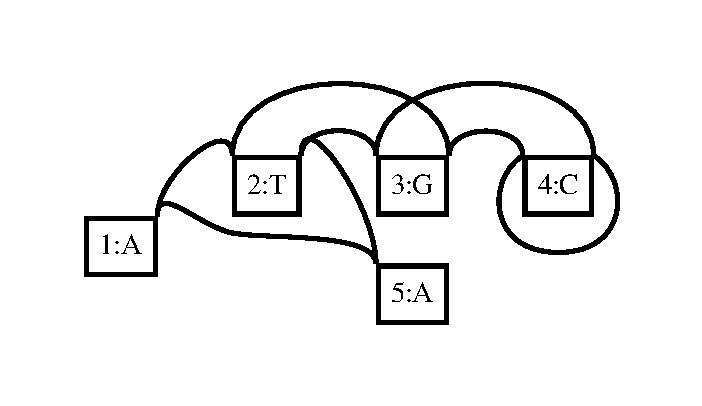
\includegraphics[width=1.0\textwidth]{Chapter2/Figs/loopy_dagify0.pdf}
    \caption{$k=0$} \label{subfig:dagify_k0}
  \end{subfigure}
  \begin{subfigure}[t]{0.49\textwidth}
    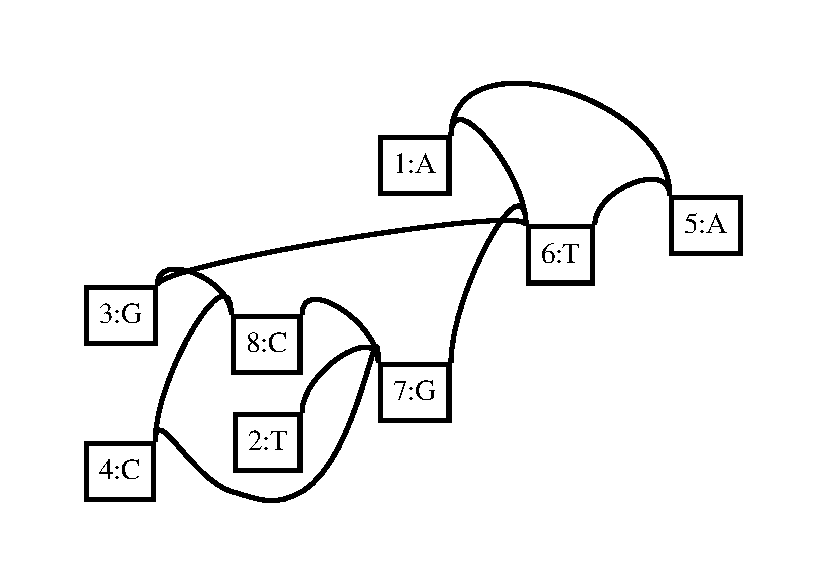
\includegraphics[width=1.0\textwidth]{Chapter2/Figs/loopy_dagify1.pdf}
    \caption{$k=1$} \label{subfig:dagify_k1}
  \end{subfigure}
  \begin{subfigure}[t]{0.49\textwidth}
    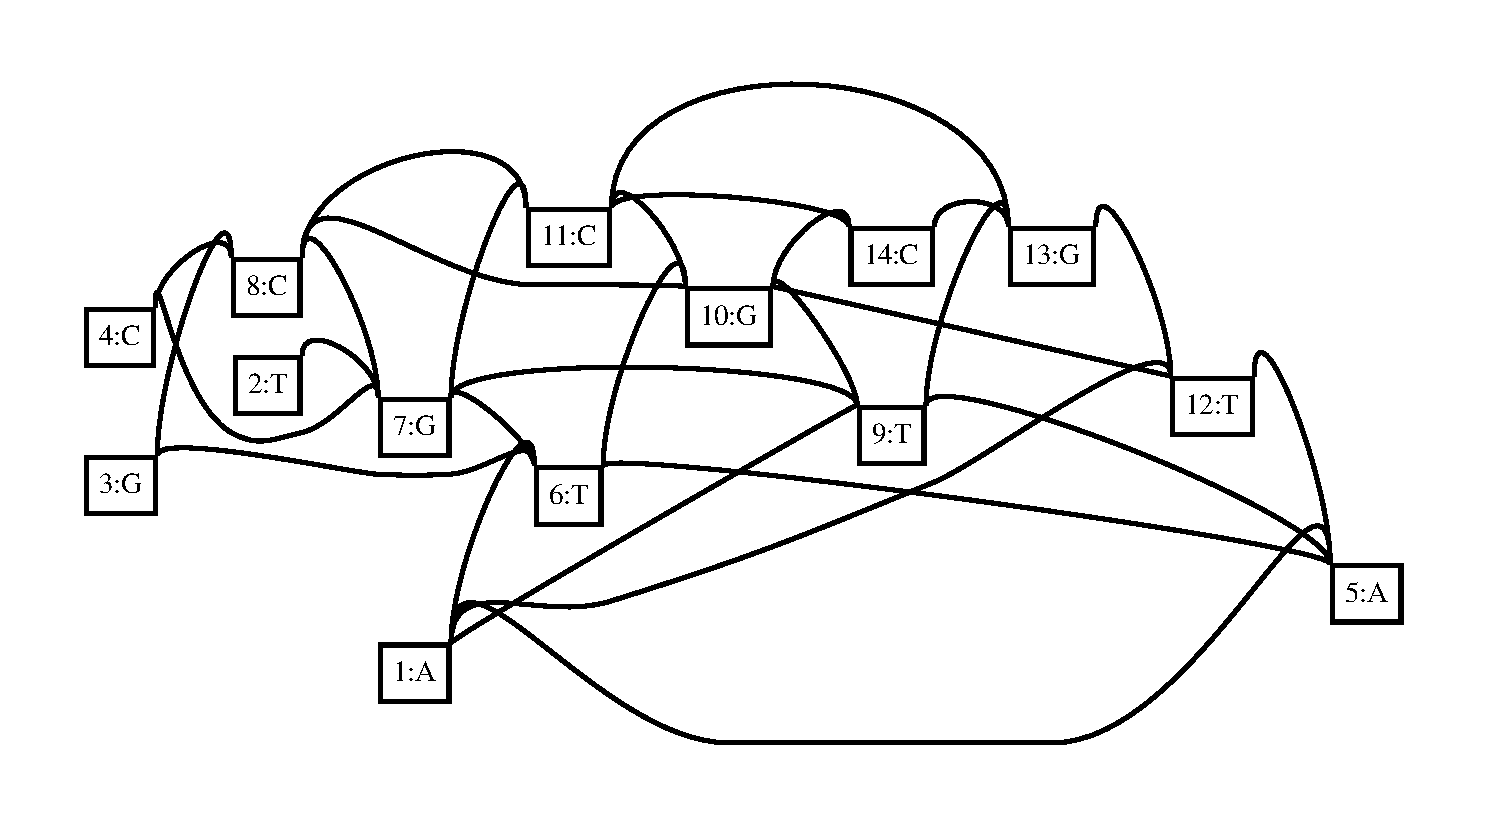
\includegraphics[width=1.0\textwidth]{Chapter2/Figs/loopy_dagify4.pdf}
    \caption{$k=4$} \label{subfig:dagify_k4}
  \end{subfigure}
  \begin{subfigure}[t]{0.49\textwidth}
    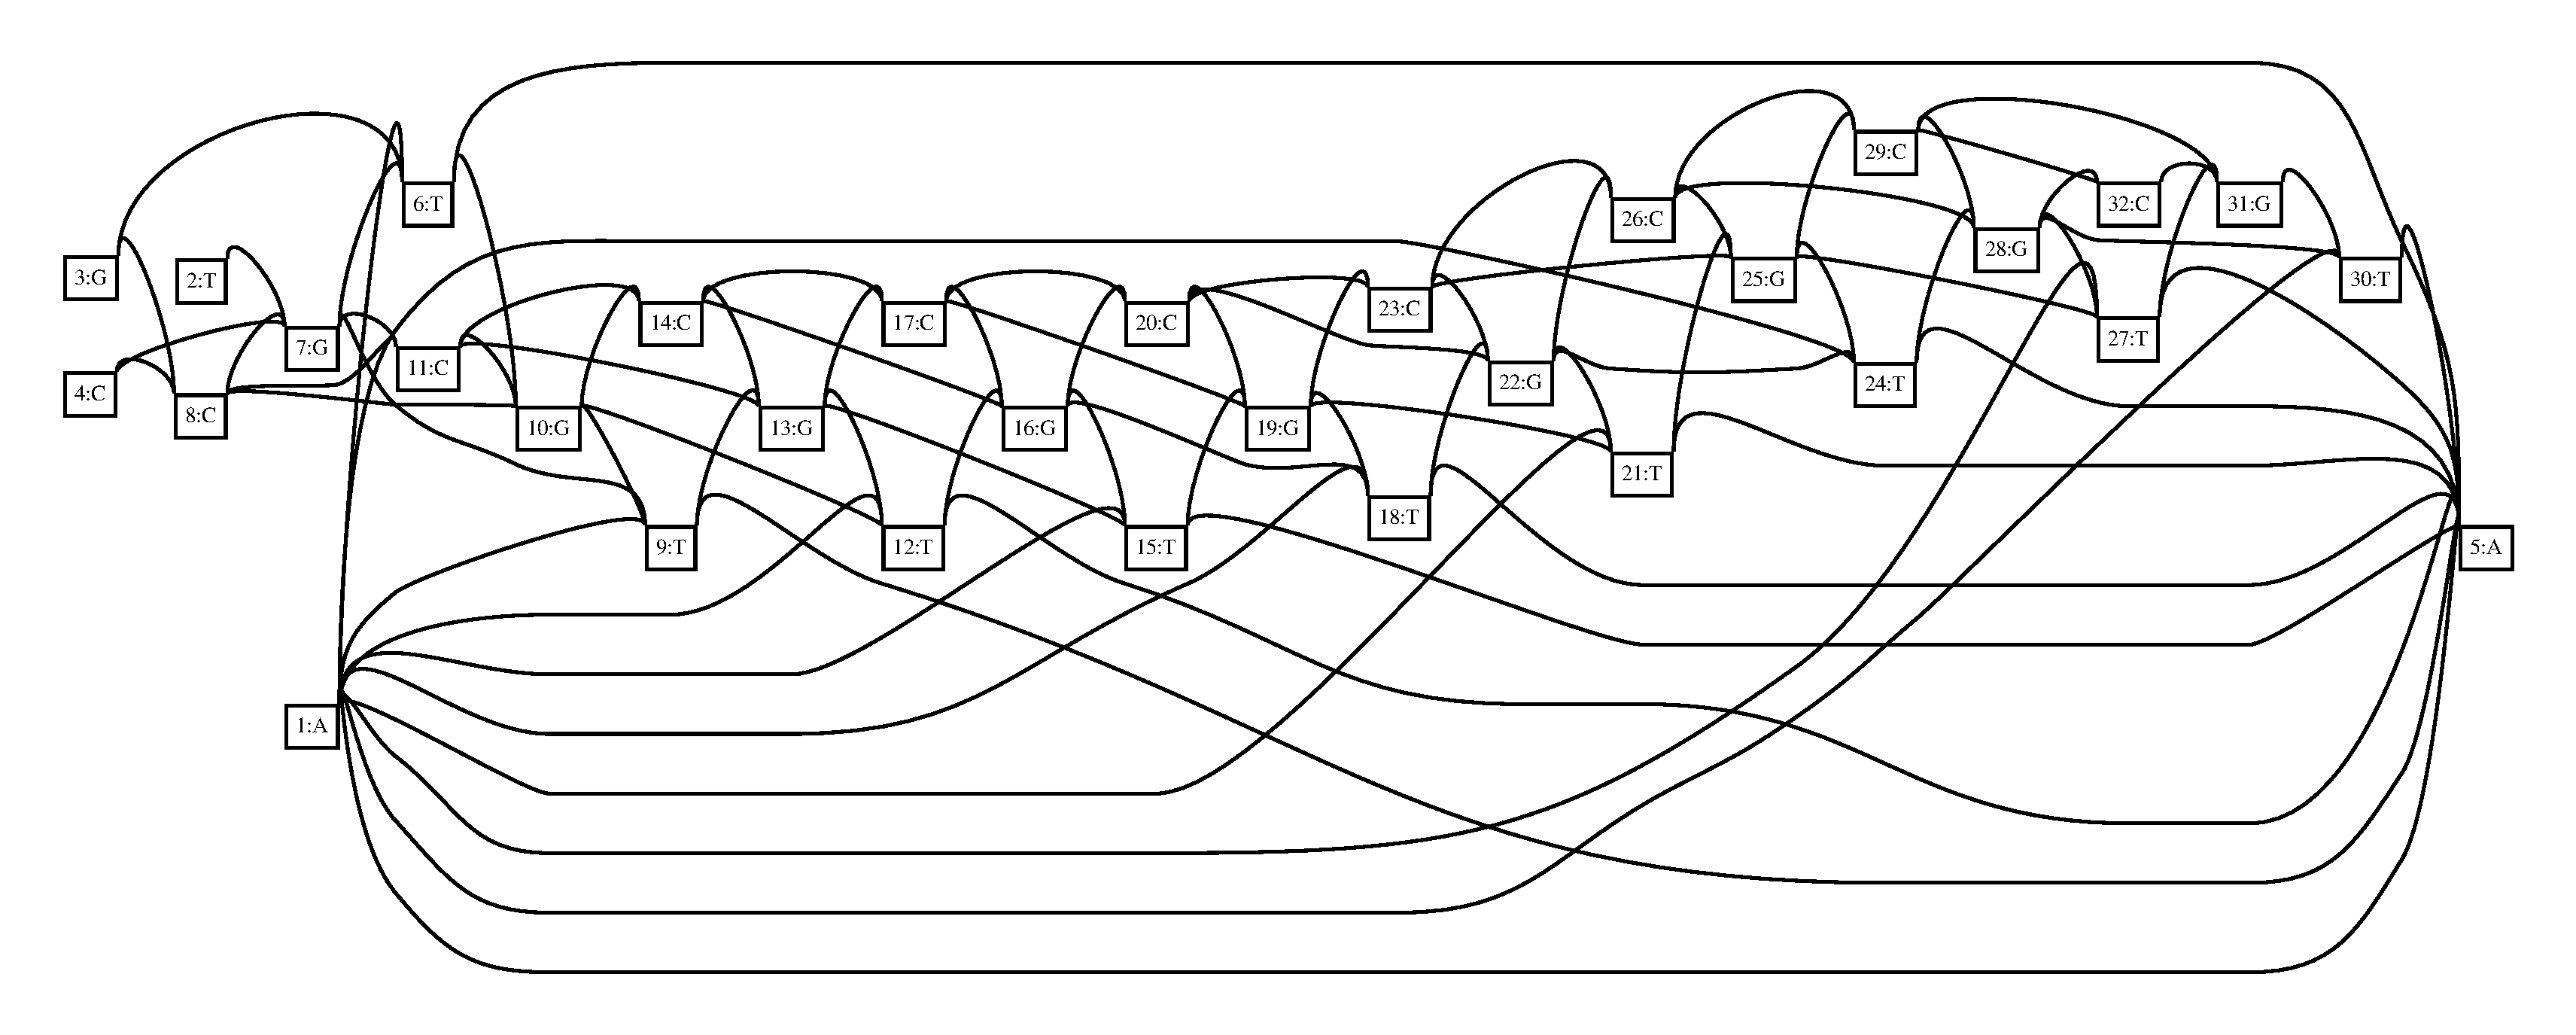
\includegraphics[width=1.0\textwidth]{Chapter2/Figs/loopy_dagify10.pdf}
    \caption{$k=10$} \label{subfig:dagify_k10}
  \end{subfigure}
  \begin{subfigure}[t]{0.49\textwidth}
    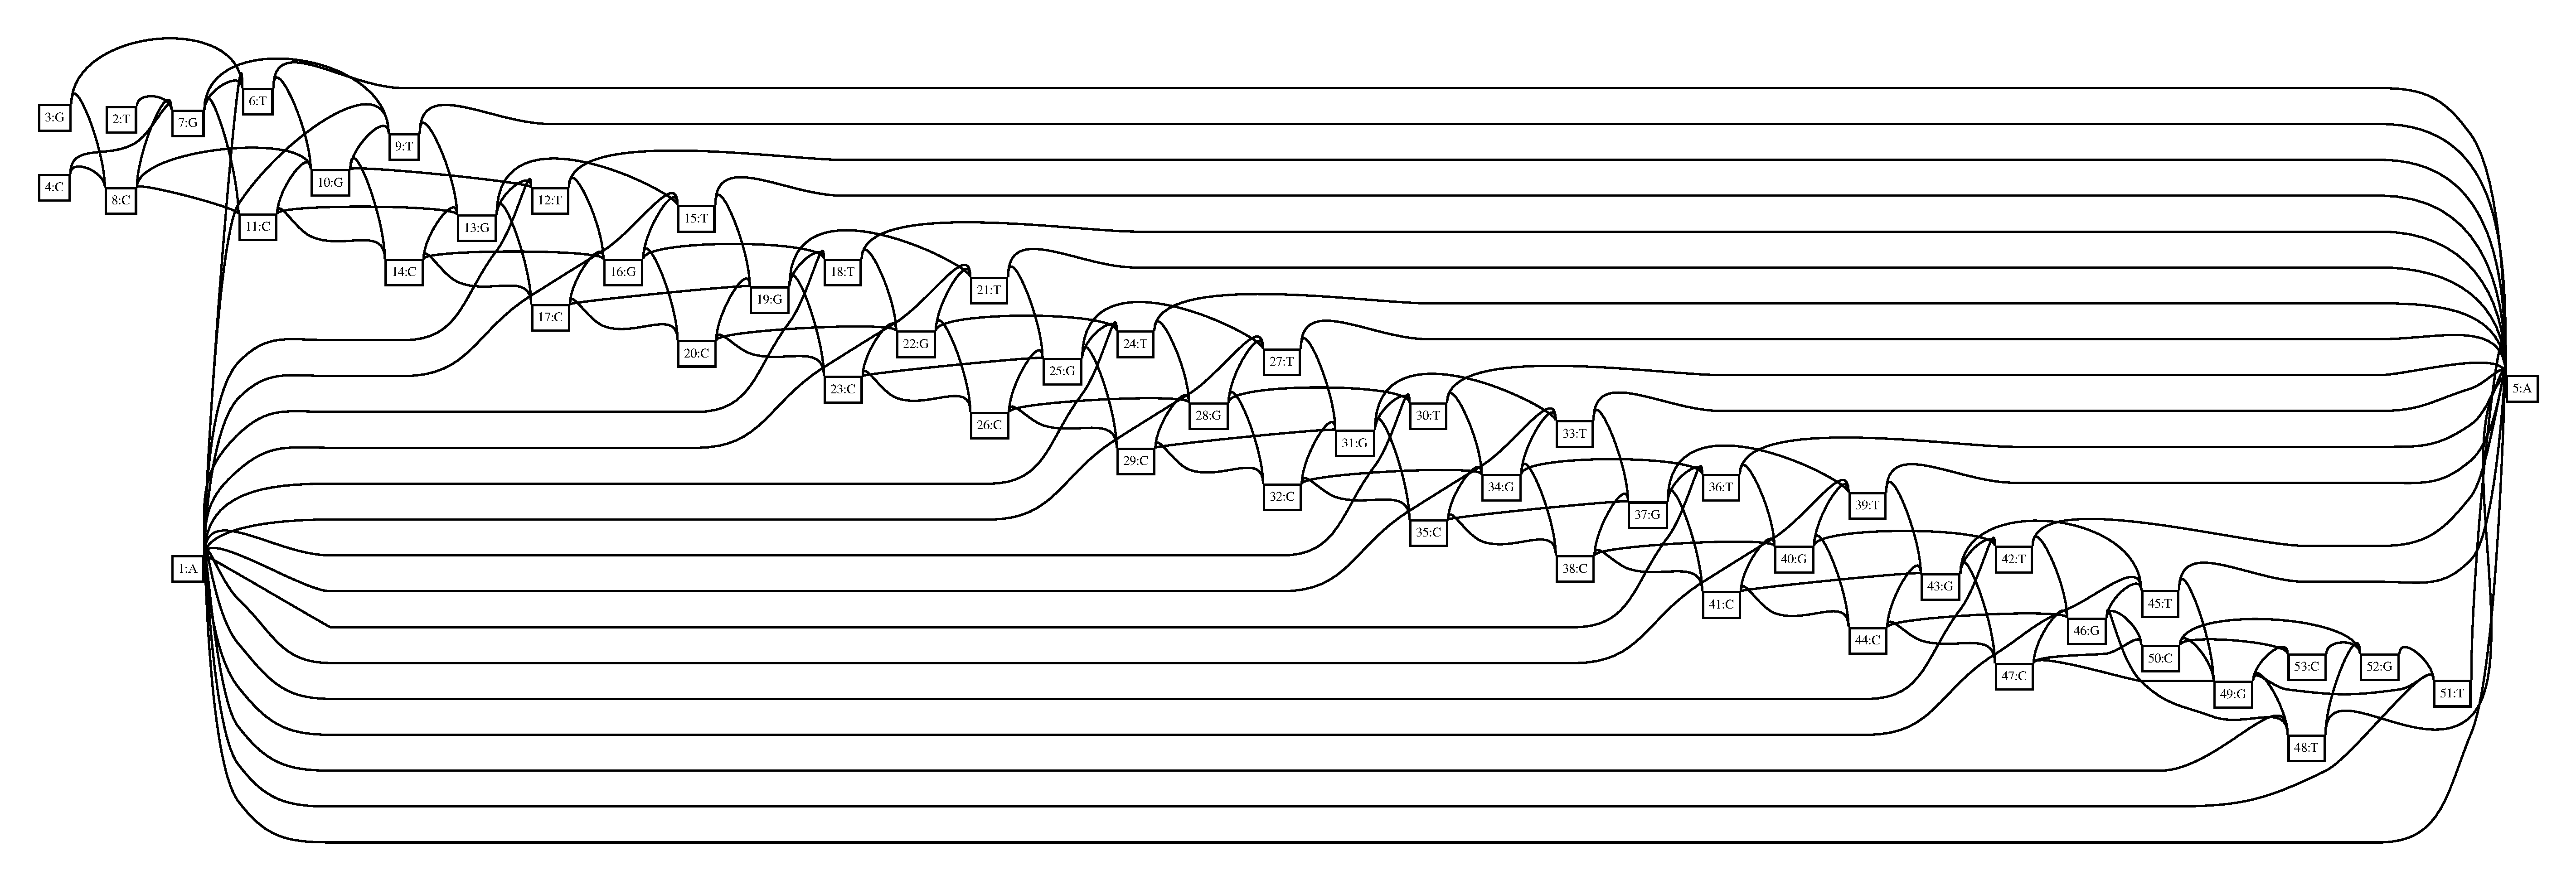
\includegraphics[width=1.0\textwidth]{Chapter2/Figs/loopy_dagify17.pdf}
    \caption{$k=17$} \label{subfig:dagify_k17}
  \end{subfigure}
  \begin{subfigure}[t]{0.49\textwidth}
    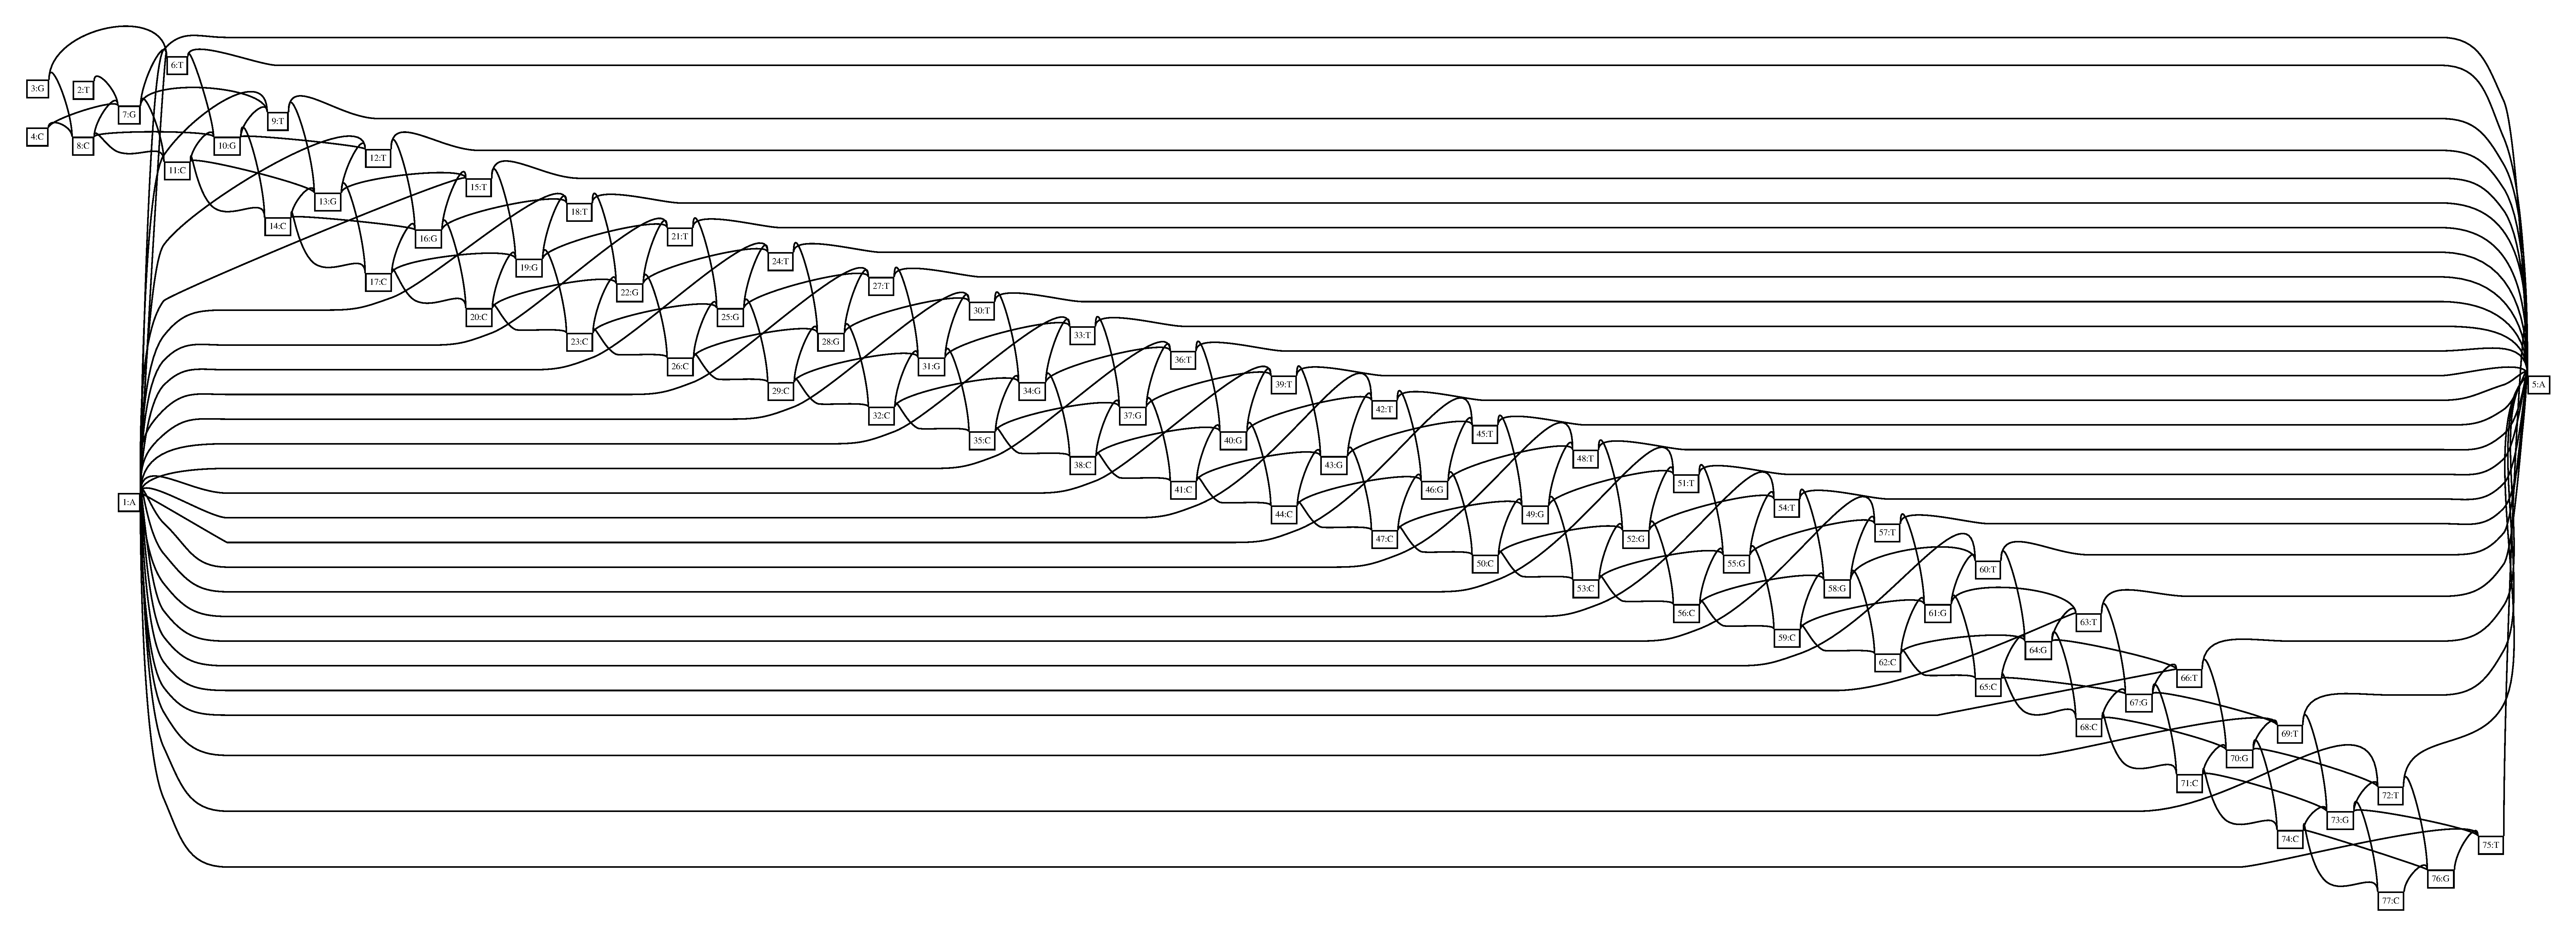
\includegraphics[width=1.0\textwidth]{Chapter2/Figs/loopy_dagify25.pdf}
    \caption{$k=25$} \label{subfig:dagify_k25}
  \end{subfigure}
  \caption[DAGification]{
    DAGification of a small graph, as seen in \ref{subfig:dagify_k0}, with the $k$ unrolling parameter given below each graph.
    \DIFaddbeginFL \DIFaddFL{In \ref{subfig:dagify_k0} we see a strongly connected component (SCC) of nodes 2, 3, and 4, which is copied in subsequent steps.
    Node ids in subsequent steps are not directly mapped to these original node ids.
    The DAGification algorithm proceeds by greedily breaking the cycles in this component, then copying the component and adding edges from the subsequent copy to the previous for each directed edge within the component until the minimum distance through the unrolled series of SCC copies is at least $k$.
    This minimum distance is tracked using a min-sum DP algorithm that is updated at each copy step by assigning a new minimum length for each node equal to the minimum of the previous minimum length among nodes in the previous SCC copy that it is connected to, plus their sequence label length.
    In panels \ref{subfig:dagify_k10}, \ref{subfig:dagify_k17}, and \ref{subfig:dagify_k25}, we see the unrolled SCC forming a braid in the middle of the rendered graphs, whose length increases with the increase in $k$.
    This algorithm is not optimal, as can be seen by the duplication of paths connecting in and out of the component.
    However it is linear, and requires only $O(kc)$ time and space, with $c$ representing a constant factor related to the size of the SCCs in the original graph.
  }\DIFaddendFL }
\label{fig:dagify}
\end{figure}

\subsection{POA and GSSW}
\DIFaddbegin \label{sec:gssw}
\DIFaddend %*2p 2h*

\emph{Graph striped Smith-Waterman} (GSSW)\footnote{\url{https://github.com/vgteam/gssw}} generalizes an implementation \cite{zhao2013ssw} of Farrar's SIMD-accelerated striped Smith Waterman (SSW) algorithm \cite{farrar2007striped} to enable string to graph alignment.
Single-Input Multiple-Data (SIMD) instructions allow vectorized mathematical operations in a single machine instruction, and can be used to greatly speed up algorithms which can be implemented in terms of operations on vectors.

GSSW generalizes all aspects of SSW to operate over sequence directed acyclic graphs, including affine gap penalties, and retains its matrices for traceback\footnote{SSW discards these matrices for performance reasons, instead establishing the traceback later with local banded DP.}.
This is simple to accomplish if the reference is a graph, as the striping of SIMD calculations in SSW across the reference is done by a single character at a time, and thus boundaries between nodes do not split the SIMD embedded variables.
We can generalize SSW to GSSW by extending the recurrence relation that defines the scores in the DP matrices to consider all previous positions on all nodes that connect to the current one.

Given a query $Q$ and a sequence graph $G = (N, E)$ with sequence length $L=\sum_{i}^{|N|} |seq(n_i)|$.
We record the maximum scores of partial alignments between $Q$ and $G$ in the set of matrices ${\cal H} = {\cal H}_1 \ldots {\cal H}_{|N|} :$ each ${\cal H}_i$ is a $|seq(n_i)| \times |Q|$ matrix.
${\cal H}$ thus contains $|Q|\times L$ cells.
When we have completed the scoring phase of alignment each ${\cal H}_{i}[x,y]$ will record the maximum score of an alignment between $Q$ and $G$ ending at $(n_i[x], Q[y])$\footnote{Here I will use brackets $[\ldots]$ to identify the cells in 2-dimensional arrays.}.
To develop our scores, we use a scoring function $score(a, b)$, which in the case of DNA returns the value of a match (typically a positive integer) when $a = b \lor a = N \lor b = N$ and the value of mismatch when $a \neq b$ (typically a negative integer).
We score a gap beginning with $\omega_\textbf{open}$ and a gap extension as $\omega_\textbf{extend}$.
We record the score of a gap along $G$ in matrices ${\cal E} = {\cal E}_1 \ldots {\cal E}_{|N|}$ and a gap along $Q$ in matrices ${\cal F} = {\cal F}_1 \ldots {\cal F}_{|N|}$.

Gaps in $\hat{\cal E}$ extend across the graph, and so we need to consider all the inbound edges when we are at the beginning of a node:

\begin{equation}
  {\cal E}_i[x,y] = \max
  \begin{cases}
    {\cal E}_i[x,y-1] - \omega_\textbf{extend} \\
    {\cal H}_i[x,y-1] - \omega_\textbf{open} \\
    \max_{\forall j : \exists e_{ji} \in E} {\cal E}_j[|n_j|,y-1] - \omega_\textbf{extend} & \text{if } x = 1 \\
    \max_{\forall j : \exists e_{ji} \in E} {\cal H}_j[|n_j|,y-1] - \omega_\textbf{open} & \text{if } x = 1 \\
  \end{cases}
\end{equation}

However, this is not the case for $\hat{\cal F}$, whose data dependencies flow vertically over the query $Q$:

\begin{equation}
  {\cal F}_i[x,y] = \max
  \begin{cases}
    {\cal F}_i[x-1,y] - \omega_\textbf{extend} \\
    {\cal H}_i[x-1,y] - \omega_\textbf{open} \\
  \end{cases}
\end{equation}


The score in $\hat{\cal H}$ combines the affine gap calculations in $\hat{\cal E}$ and $\hat{\cal F}$.
As with $\hat{\cal E}$, we here we also must consider the inbound nodes:

\begin{equation}
  \label{eqn:gssw_h}
  {\cal H}_i[x,y] = \max
  \begin{cases}
    0 \\
    {\cal E}_i[x,y] \\
    {\cal F}_i[x,y] \\
    {\cal H}_i[x-1,y-1] - score(Q[x], n_i[y])\\
    \max_{\forall j : e_{ji} \in E} {\cal H}_j[|n_j|,y-1] - score(Q[x], n_j[y]) & \text{if } x = 1 \\
  \end{cases}
\end{equation}

The values of ${\cal H}_i$, ${\cal E}_i$, and ${\cal F}_i$ are 0 when $x = 0$ or $y = 0$ and node $n_i$ has no inbound edges.
Note that this is the initial condition provided by Gotoh to improve the algorithm of Smith and Waterman.

We fill the matrices using Farrar's SSW algorithm \cite{farrar2007striped}, based on Zhao's implementation \cite{zhao2013ssw}.
By storing the full score matrices we can then trace back from the maximum score in $\hat{\cal H}$ to obtain the optimal alignments under our scoring parameters.
The traceback can be represented as moves in the matrix, or equivalently as the alignment object model described in section \ref{sec:alignments}.

\subsection{Banded global alignment and multipath mapping}
\label{sec:banded_global}

By modifying equation \ref{eqn:gssw_h} so that it is no longer lower-bounded at 0 and changing the traceback so that it goes from beginning to end of query $Q$ and graph $G$, we obtain a ``global'' alignment algorithm with the same properties as Needleman-Wunsch.
To reduce computational costs, we can \emph{band} the algorithm to limit the region of the DP tables which needs to be explored.
This approach, as implemented in {\tt vg} by Jordan Eizenga, forms the basis for multipath mapping, in which alignments are represented probabilistically as DAGs rather than linear series of node traversals and edits.
In multipath mapping, regions between MEMs in a particular cluster are aligned using global alignment.
The use of global alignment ensures that the alignment fully covers the gap between the MEMs.
Multiple traceback allows for alternatives to be included, and each of these may be scored on the basis of both alignment score and haplotype matching score.
His implementation is key to the development of haplotype aware mapping, which is the subject of a paper currently in preparation by myself and collaborators on the {\tt vg} project.
In the case of low-error reads, this limited exploration of the DP problem allows for fast derivation of the optimal alignments, and so the multipath mapper in {\tt vg mpmap} achieves runtime comparable to or exceeding {\tt vg map}.
Multipath mapping concepts also form the basis for alignment surjection, in which an alignment to the graph is projected into the linear reference.

\subsection{X-drop DP}

As our query length $|Q|$ increases, so does the practical complexity of deriving the alignment using POA/GSSW.
We align longer queries against larger graphs, and so we effectively face a quadratic penalty with increasing alignment length, $|Q| \propto |L| \implies$ GSSW is $O(|Q|^2)$.
The most direct solution to this is to use a banded alignment method like banded global alignment, as described in section \ref{sec:banded_global}.
However, this method cannot exploit data parallel operations that allow dramatic speedups on modern processors.

In the course of our work on {\tt vg}, Eizenga and I explored the application of Hajime Suzuki's adaptive banded global alignment (libgaba)\footnote{\url{https://github.com/ocxtal/libgaba}} \cite{suzuki2017acceleration}, which has been used in {\tt minimap2} to greatly improve alignment speed with long single-molecule reads \cite{li2018minimap2}.
In this approach, an antidiagonal band of cells is computed at each step, of a predetermined width designed to fit into the word sizes of SIMD instructions.
The band can move either ``right'' or ``down'' at each step, depending on where the highest score is found.
A termination criterion is given, so that alignment stops when the maximum score falls a given amount.
This is similar to the X-drop parameter used in BLAST to stop alignment extension.
Although it improves performance, it can hurt sensitivity to indels.

Suzki had already implemented a version of alignment over graphs by transforming the graph into a tree through a dynamic unrolling process akin to that described in \ref{sec:DAGify} and aligning to the tree using libgaba\footnote{\url{https://github.com/ocxtal/comb}}.
His implementation supports graph to graph alignment as described in section \ref{sec:translation}, but the exponential expansion of the alignment problem on trees is fundamentally limiting.
Eizenga, Suzuki and I discussed methods to merge the bands together after traversal of unifications in the graph, but we could not establish a safe generic method to merge them.
Furcated bands may only be merged directly if they map to the same query coordinate.
This is unlikely to happen if the different paths in the graph that they have traversed have different lengths or if there are indels in the alignment.

During a biohackathon meeting in Kyoto, Suzuki presented an alternative banding model based on the ``X-drop DP'' algorithm from BLAST.
In this model, the alignment is matrix broken into vertical non-striped windows that tile across the DP matrices over fixed subsequences in the query.
To efficiently resolve the data dependencies between successive steps, a SIMD shuffle operation is applied to the cell values stored in each window.
Forward progression of each window stops when the highest score in the forefront cells drops $X$ below the previously-observed maximum.
This approach thus allows the band to spread as wide as needed to accommodate larger insertions, while being bounded by the $X$-drop parameter.
The result is an approach that is more sensitive than the antidiagonal banded alignment in libgaba, but runs a factor of 2 slower for equivalent band sizes.

\begin{figure}[htbp!] 
\centering    
\DIFdelbeginFL %DIFDELCMD < 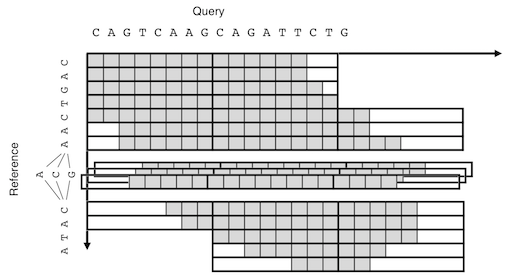
\includegraphics[width=0.65\textwidth]{Chapter2/Figs/xdrop.png}
%DIFDELCMD < %%%
\DIFdelendFL \DIFaddbeginFL 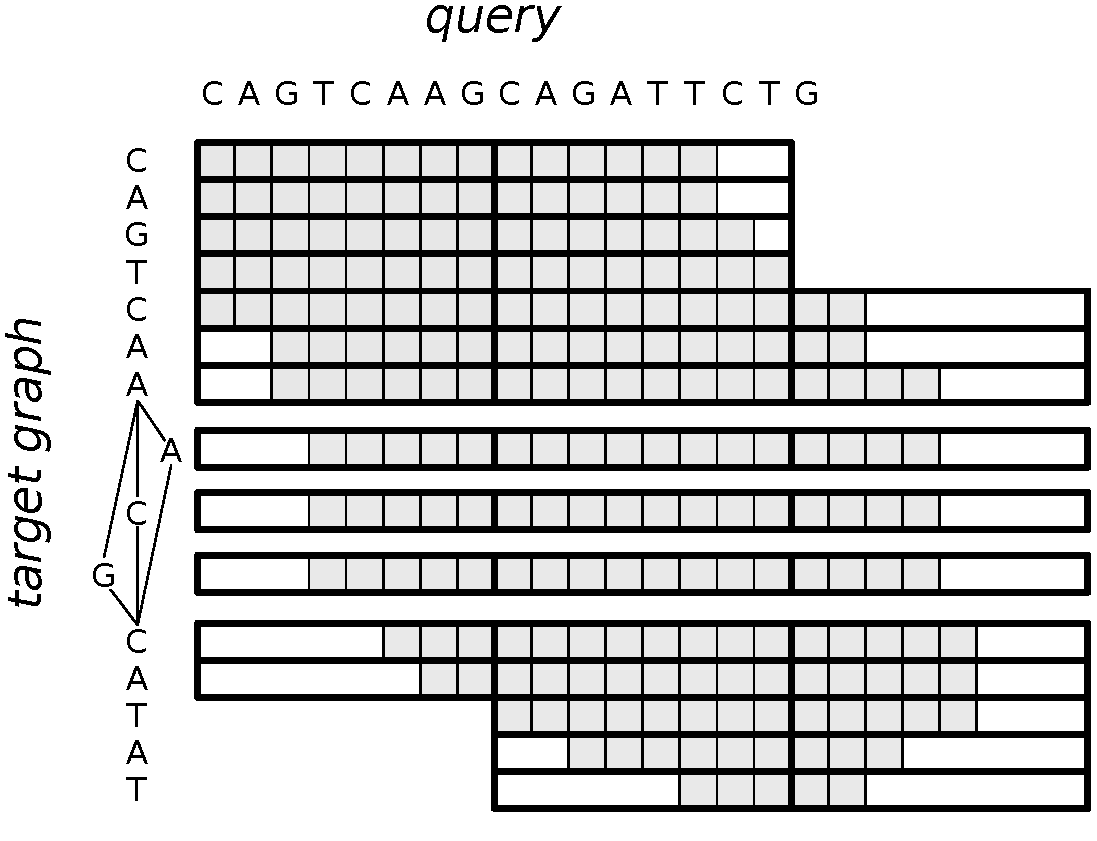
\includegraphics[width=1.0\textwidth]{Chapter2/Figs/xdrop.pdf}
\DIFaddendFL \caption[The \emph{dozeu} X-drop alignment algorithm]{
  \DIFdelbeginFL \DIFdelFL{The }\DIFdelendFL \DIFaddbeginFL \DIFaddFL{Evaluation of the }\DIFaddendFL \emph{dozeu} X-drop alignment algorithm \DIFdelbeginFL \DIFdelFL{.
  Black rectangles represent the evaluated region of the score matrix, which each box corresponding to a SIMD vector value}\DIFdelendFL \DIFaddbeginFL \DIFaddFL{for an example graph}\DIFaddendFL .
  Grey cells represent the part of the score matrix for which our X-drop parameter would allow evaluation if we were calculating the matrix one cell at a time.
  \DIFdelbeginFL \DIFdelFL{Reprinted }\DIFdelendFL \DIFaddbeginFL \DIFaddFL{8-cell wide black rectangles that contain the full set of grey cells represent the region of the score matrix for which we calculate scores when using a SIMD-based accelerated version of the algorithm.
  Traceback and per-cell scores are not shown.
  This figure is meant to illustrate the adaptive banding property of the X-drop algorithm and how that can be used in a SIMD-based acceleration of the algorithm.
  Adapted }\DIFaddendFL with permission from \url{https://github.com/ocxtal/dozeu}.
}
\label{fig:xdrop}
\end{figure}

I have since worked with Suzuki to integrate his implementation of this algorithm \emph{dozeu}\footnote{\url{https://github.com/ocxtal/dozeu}} into {\tt vg}.
Due to difficulties in handling paired end rescue, the approach is not yet performing as well as GSSW for {\tt vg map}.
This remains a work in progress, but is a promising approach to enable the direct alignment of long sequences against the graph.
It is orthogonal to the ``chunked'' alignment approach, and in principle, they can be applied together to build a SV-aware, chunked and banded alignment process.
Future work in this direction may yield a new VG alignment algorithm, but this lies outside the scope of this thesis.

\subsection{Chunked alignment}
%*1p 1h*
\label{sec:chunked_alignment}

For long reads, where in the worst case the local dynamic programming can become prohibitively expensive, we break the reads into ``bands'' of a fixed width $w$ (default 256 base pairs) with overlap between successive bands of $w/8$.
\DIFaddbegin \DIFadd{Chunking the alignment process allows us to directly detect complex structural variation within our alignment, and provides a kind of split read alignment model for }{\tt \DIFadd{vg}}\DIFadd{.
}\DIFaddend We align these bands independently, trim the overlaps from the alignments, and build \DIFdelbegin \DIFdel{a Markov model from them }\DIFdelend \DIFaddbegin \DIFadd{an alignment DAG model $G_\textsc{AlignChain} = (N, E)$ }\DIFaddend similar to that built for MEM chaining \DIFdelbegin \DIFdel{, only that here }\DIFdelend \DIFaddbegin \DIFadd{(as in \ref{sec:collinear_chaining}).
The only significant difference between these two models is that in $G_\textsc{AlignChain}$, }\DIFaddend we consider sub alignments as nodes in the model rather than MEMs.
\DIFaddbegin 

\DIFaddend In this model we put weights on transitions between alignments that relate to the estimated distance between the alignments in the graph versus their distance in the read, with the objective of making long co-linear chains be the highest-scoring walks through the \DIFdelbegin \DIFdel{Markov }\DIFdelend \DIFaddbegin \DIFadd{chaining }\DIFaddend model.
We take the \DIFdelbegin \DIFdel{Viterbi }\DIFdelend \DIFaddbegin \DIFadd{max-sum }\DIFaddend path through the model to be the best alignment.
Then, to obtain multiple alignments, we mask out this path, re-score, and take the \DIFdelbegin \DIFdel{Viterbi }\DIFdelend \DIFaddbegin \DIFadd{next max-sum }\DIFaddend path to get the 2nd-, 3rd-, and ultimately $N$th-best alignment.
\DIFaddbegin 

\DIFaddend After they have been extracted from the model, alignments are ``patched'' using local alignment of unaligned regions anchored in the graph near the end of previous mapped regions, so that sub-alignments which may have been misaligned due to repeats may be locally aligned correctly.
\DIFdelbegin \DIFdel{Although this sounds complex, in a very high fraction of cases neighboring alignments overlap exactly in the overlap region of size w/8, and chaining is trivial.
}\DIFdelend This model allows {\tt vg} to map noisy reads of arbitrary length, and is used as a core component in the long read progressive assembler {\tt vg msga}.

\DIFaddbegin \DIFadd{Although the development of $G_\textsc{AlignChain}$ is very similar to $G_\textsc{MemChain}$, but a number of important differences distinguish the two models.
For clarity, I will fully exposit the chunked alignment chaining model here, despite its strong similarity to the MEM chaining model.
}

\begin{figure}[htbp!]
\centering
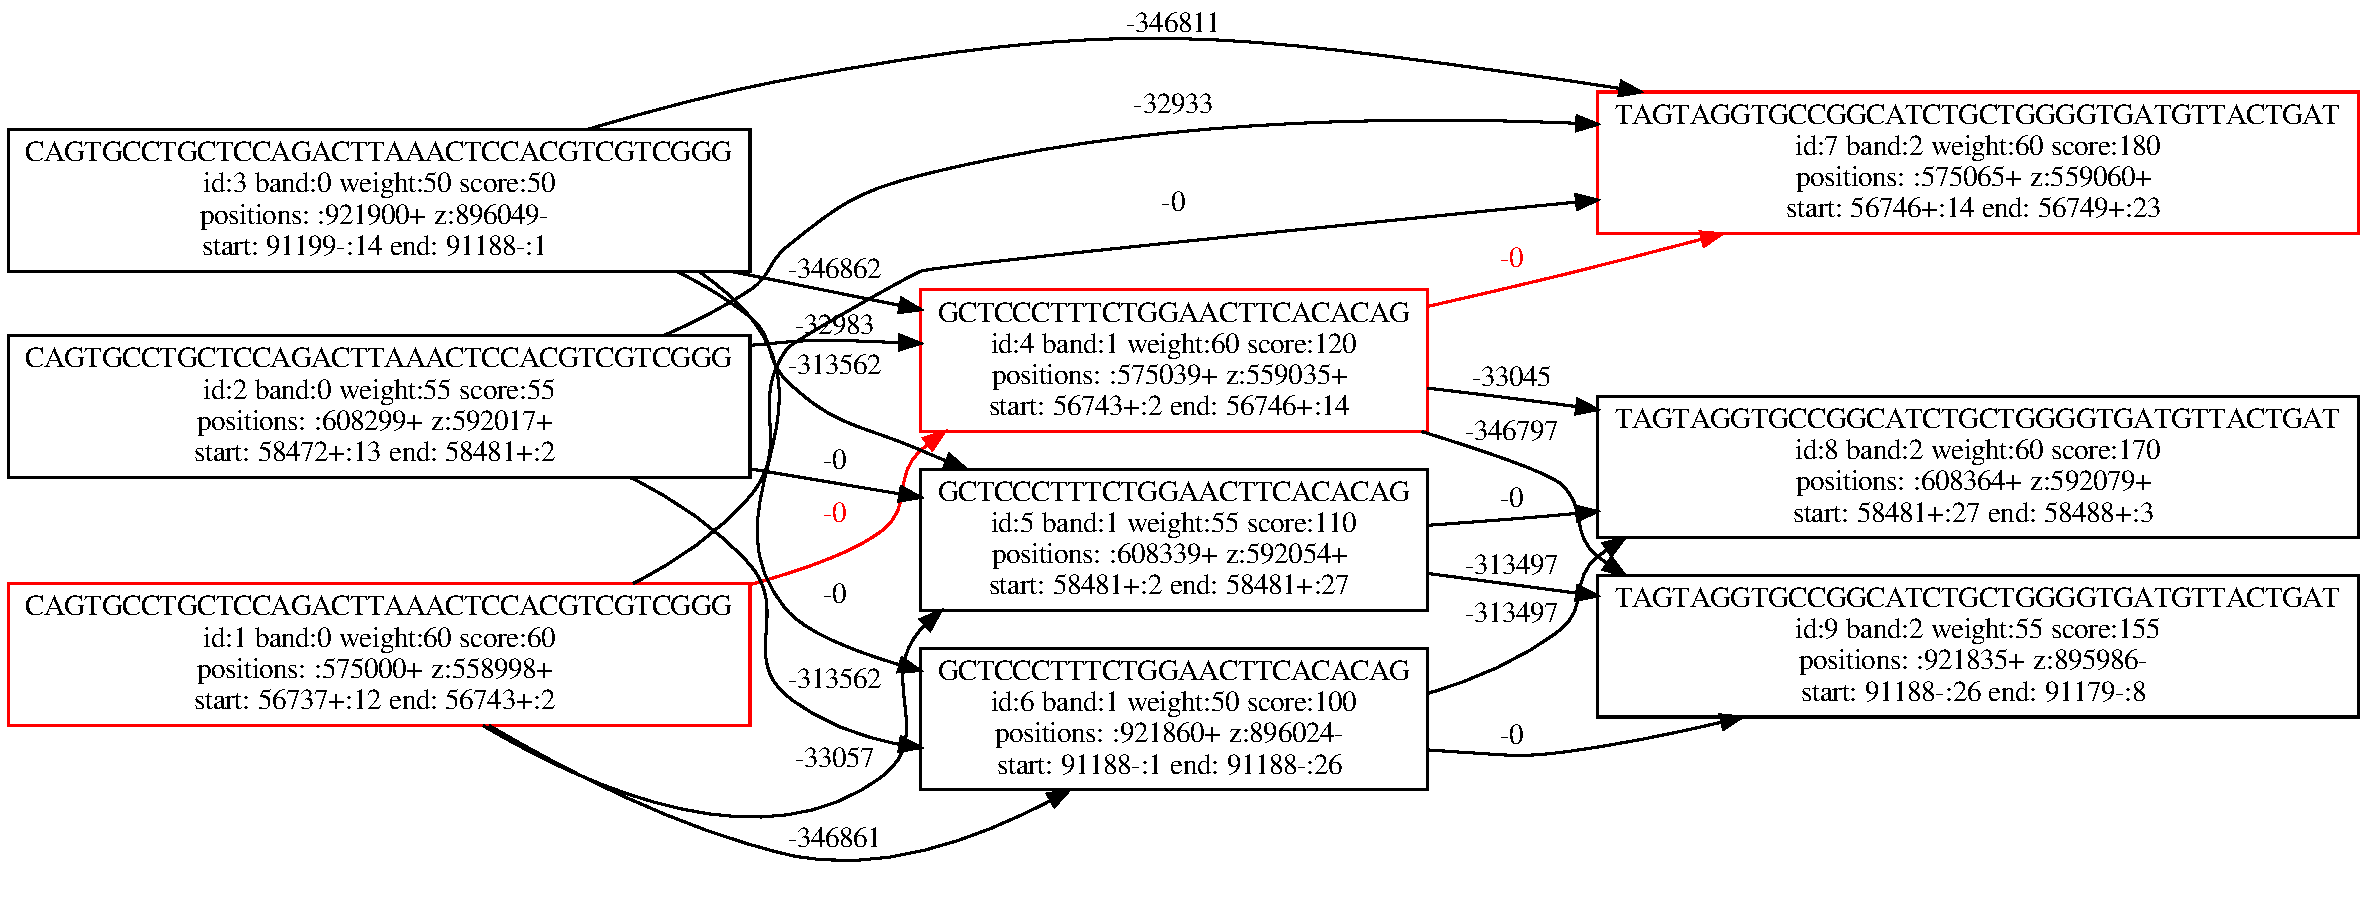
\includegraphics[width=1.0\textwidth]{Chapter2/Figs/alignchain_dag.pdf}
\caption[The Alignment Chain Model]{
  \DIFaddFL{The first evaluation of the alignment chain model for a set of alignment bands derived from a simulated query mapped against a test 1Mbp 1000GP graph included in the }{\tt \DIFaddFL{vg}} \DIFaddFL{repository, using }{\tt \DIFaddFL{vg map}} \DIFaddFL{parameters }{\tt \DIFaddFL{-w 50 -O 25 -J 2}} \DIFaddFL{to simplify the model for exposition.
  Each node refers to a single mapping of an alignment band, its sequence, weight, its band index among bands taken from the original query, a node id in the graph, and the score derived from the first pass of the max-sum algorithm.
  %DIF > Each of the three bands has been aligned to three locations in the reference graph, resulting in three columns of nodes, with each column corresponding to a given band.
  Edges are labeled with their derived weight ${\cal W}_{e_{ij}}$, which can be seen to be 0 for edges connecting bands whose end and start positions directly connect.
  The maximum scoring chain is shown in red, and corresponds to the correct mapping location of the simulated query.
}}
\label{fig:alignmentchain_model}
\end{figure}


\DIFadd{As each subalignment is part of the full alignment that we'll derive by finding the max-sum path through the model, we apply use the alignment score to set the initial weight for the node:
}

\begin{equation}
  {\DIFadd{\cal W}}\DIFadd{_{n_i} = alignment\_score(n_i)
}\end{equation}

\DIFadd{Each alignment node $n_i$ has a set of graph start and end positions $graph\_start\_pos(n_i) = \{ b_1 \ldots b_m \}$, $graph\_end\_pos(n_i) = \{ b_1 \ldots b_m \}$.
We use these to provide weights for the edges in the alignment chain model.
Edges $e_{ij}$ in $G_\textsc{AlignChain}$ represent possible transitions between sub-alignments, and are weighted (${\cal W}_{e_{ij}}$) by the minimum estimated distance between the given graph positions for each alignment end, times the gap open and extension costs.
The alignment bands overlap during the alignment of each sub-alignment, but at the point when we establish the model, we have trimmed the overlaps butween successive sub-alignments and re-calculated the alignment score, so we do not need to consider them here.
Unlike the MEM chaining model, which is driven entirely by approximate distances, when we obtain an estimated distance less than the length of the alignment chunk, we walk the graph using a depth first search in order to obtain a precise minimum value for the distance.
}

\begin{equation}
  \DIFadd{dist_{e_{ij}} = \min_{dist(b,d)} \forall b \in graph\_end\_pos(n_i), \forall d \in graph\_start\_pos(n_j)
}\end{equation}

\DIFadd{The chunked alignment model allows us to align through inversions, which we score using a basic heuristic that they are twice as costly as a gap of the same length as the inverted sequence.
The inversion distance estimate walks forward from the positions in $n_j$ and seeks $n_i$.
In the case of a non-inversion, the resulting estimate will be $\infty$, as $n_i$ will never be reached by walking forward from $n_j$.
}

\begin{equation}
  \DIFadd{dist\_inv_{e_{ij}} = dist_{e_{ji}}
}\end{equation}

\begin{equation}
  {\DIFadd{\cal W}}\DIFadd{_{e_{ij}} = \max
  \begin{cases}
    \omega_\textbf{extend} dist_{e_{ij}} + \omega_\textbf{open} [dist_{e_{ij}} \ne 0] \\
    2 \times \left( \omega_\textbf{extend} dist\_inv_{e_{ij}} + \omega_\textbf{open} [dist\_inv_{e_{ij}} \ne 0] \right)
  \end{cases}
}\end{equation}

\DIFadd{These node and edge weights relate to the final alignment score that we would expect should we concatenate a particular series of sub-alignments.
%DIF > We expect a positive score due to an exact match, so we apply a positive weight to each node as it represents a MEM.
%DIF > Transtions between sub-alignments may encode gaps or mismatches.
We cannot precisely estimate the final score of the read without the final patching step, but we can use our position index and the function $dist(b,d)$ to estimate gap lengths.
We take the score of a concatenated alignment ${\cal P} = n_i \ldots n_j$ in the model to be:
}

\begin{equation}
  {\DIFadd{\cal S}}\DIFadd{_{\cal P} = \sum_{i = 0}^{|{\cal P}|-2} }{\DIFadd{\cal W}}\DIFadd{_{{\cal P}[i]} + }{\DIFadd{\cal W}}\DIFadd{_{e_{{\cal P}[i]{\cal P}[i+1]}}
}\end{equation}

\DIFadd{Given this definition, we expect the maximum sum walk ${\cal P}_\textsc{max} = n_i \ldots n_j$ through the graph to be likely to yield the series of sub-alignments and graph positions involved in the maximum scoring alignment we would obtain should we have aligned the entire query in one step.
This concatenated alignment is approximate due to the incompleteness of our score estimate and the fact that our alignment set is not guaranteed to capture the optimal alignment due to the arbitrariness of the banding pattern that we have applied.
Incompleteness due to our partitioning of the alignment problem means that to obtain a precise score we must locally realign unaligned portions of the concatenated alignment.
This alignment patching process resolves problems that can occur due to induced soft clips, fully unaligned bands, or structural variations such as inversions or small CNVs that frustrate the complete alignment of a particular band.
}

\DIFadd{As with the MEM chaining model, we derive partial alignments from $G_\textsc{AlignmentChain}$ by applying a standard max-sum dynamic programming algorithm to derive the maximum possible final alignment score at each node, and then, by working from the maximum scoring node, derive the maximum scoring path through the graph.
The score for each node ${\cal S}_{n_i}$, combines the sum of own weight, the maximum score of any previous node it is connected to, and the weight of the edge connecting the maximum scoring inbound node and the current node:
}

\begin{equation}
  {\DIFadd{\cal S}}\DIFadd{_{n_i} = }{\DIFadd{\cal W}}\DIFadd{_{n_i} + \max_{\forall e_{ji} \in E} \left( }{\DIFadd{\cal W}}\DIFadd{_{e_{ji}} + }{\DIFadd{\cal S}}\DIFadd{_{n_j} \right)
}\end{equation}

\DIFadd{To allow traceback of the maximum scoring path, we record the maximum inbound node for each node.
}

\begin{equation}
  {\DIFadd{\cal T}}\DIFadd{_{n_i} = \operatorname*{argmax}_{n_j} \left( }{\DIFadd{\cal W}}\DIFadd{_{e_{ji}} + }{\DIFadd{\cal S}}\DIFadd{_{n_j} \right)
}\end{equation}

\DIFadd{At the end of the scoring phase, we find the highest scoring node.
}

\begin{equation}
  \DIFadd{n_{max} = \max_{\forall n_i \in N} }{\DIFadd{\cal S}}\DIFadd{_{n_i}
}\end{equation}

\DIFadd{Walking back through the series of recorded traceback pointers yields the maximum scoring concatenated alignment under the alignment scoring and transition weight model we've applied.
We define the series of nodes in the max-sum path by $n_{max-i-1} = {\cal T}_{n_{max-i}}$.
The resulting path is expressed in reverse order relative to our traceback.
}

\begin{equation}
  {\DIFadd{\cal P}}\DIFadd{_\textsc{max} = n_{max-|{\cal P}_\textsc{max}|} \dots n_{max-1}, n_{max}
}\end{equation}



\DIFaddend \subsection{Alignment surjection}
\DIFaddbegin \label{sec:surjection}
\DIFaddend 

Alignments to graphs that include linear reference sequences as paths can be transformed into alignments against those paths.
\DIFdelbegin \DIFdel{To be well-defined, this lossy transformation, }\emph{\DIFdel{surjection}}%DIFAUXCMD
\DIFdel{, }\DIFdelend \DIFaddbegin \DIFadd{Alignment }\emph{\DIFadd{surjection}} \DIFadd{projects alignments to the full graph }\emph{\DIFadd{onto}} \DIFadd{the subgraph defined by a given set of paths in the graph.
This transformation is used to convert graph based alignments to alignments to the linear reference, and is of great utility in the application of }{\tt \DIFadd{vg}} \DIFadd{in resequencing based analyses, where it supports a lossy translation between }{\tt \DIFadd{vg}}\DIFadd{'s native GAM format and BAM.
}

\DIFadd{In surjection, portions of the alignment that already map to the path specific graph subset are left unchanged.
However, regions of the original alignment to parts of the graph that are not in the selected path subset are mapped onto the nearest suitable node, with additional edits to specify the differences between the alignment and the graph subset defined by the target paths.
To produce a meaningful alignment, surjection }\DIFaddend requires that the alignment path matches the reference path for some portion of its length.
\DIFaddbegin \DIFadd{Otherwise, the resulting alignment would be empty, or unaligned.
}

\DIFadd{The name ``surjection'' is meant to be illustrative, and is not mathematically precise in the sense that it only applies to the alignments in terms of the node space of their paths.
When we consider only the set of nodes that are traversed by a given alignment and its surjection, it is given that the function is surjective, as the domain of the function is the full graph, while the codomain is the subset defined by a given set of paths, with each node corresponding to one or more nodes in the original graph.
(For instance, a mapping to a non-reference allele would be projected onto the nearest neighboring node in a reference path.)
This surjective property would be violated in the case of a graph that only consisted of nodes in the paths that we are projecting our alignments into, as in this case the projection would bijective or the identity.
}

\DIFadd{However, it is not clear that projecting the alignments into a graph subset defined by a given set of paths is surjective when we consider the full alignment data model.
Information about the original alignment sequence is fully retained in the node mappings of the surjected alignment path, and this can be seen as violating the surjective property of the transformation.
}

\DIFaddend The simplest surjection technique extracts the reference path region matching an alignment and realigns the read against it.
Doing so without global alignment will often result in soft clipping, such as where non-reference alleles in the graph have allowed full length alignment.
This can be resolved to some extent by applying global alignment of the alignment query sequence against the reference.
But a more rigorous approach rebuilds the alignment in parts.
For each piece that is not aligned to the reference, we extract the intervening reference sequence and align only the subset of the query that is no longer matching to this region.
A kind of anchored semi-global alignment may be used on the ends of the reads, where the opposite reference-matching end is not defined.
The resulting alignment may easily be expressed in the BAM format and thus be used by standard downstream variant calling and analysis methods.

\subsection{Base quality adjusted alignment}
%*2p 2h*

Base qualities are typically reported on the Phred scale so that the probability of error for a given quality $Q$ is $\epsilon = 10^{-Q/10}$. Assuming no bias in which bases are mistaken for each other, this defines a posterior distribution over bases $b$ for a base call $x$.

\begin{align}
    P(b|x, \epsilon) = \begin{cases}
        1 - \epsilon & b = x \\
        \frac{1}{3} \epsilon & b \neq x
    \end{cases}
\end{align}

We use this distribution to derive an adjusted score function. Normally, the match score for two bases is defined as the logarithm of the likelihood ratio between seeing two bases $x$ and $y$ aligned and seeing them occur at random according to their background frequencies. 

\begin{align}
    s_{x,y} &= \log\left(\frac{p_{x,y}}{q_y q_x} \right) \label{eqn:base_score}
\end{align}

Next we marginalize over bases from the posterior distribution to obtain a quality adjusted match score.

\begin{align}
    \tilde s_{x,y}(\epsilon) &= \log\left(\frac{(1 - \epsilon)p_{x,y} + \frac{\epsilon}{3}\sum_{b \neq x}p_{b, y}}{q_y\left((1 - \epsilon)q_x + \frac{\epsilon}{3}\sum_{b \neq x}q_b \right)} \right)
\end{align}

{\tt vg} works backwards from integer scoring functions to the probabilistic alignment parameters in this equation. After doing so, the match scores are given by

\begin{align}
    \tilde s_{x,y}(\epsilon) &= \frac{1}{\lambda} \log\left(\frac{(1 - \epsilon)q_x q_y e^{\lambda s_{x,y}} + \frac{\epsilon}{3}\sum_{b \neq x}q_b q_y e^{\lambda s_{b,y}}}{q_y\left((1 - \epsilon)q_x + \frac{\epsilon}{3}\sum_{b \neq x}q_b \right)} \right).
\end{align}

Here, $\lambda$ is a scale factor that can be computed from the scoring parameters, and the background frequencies $q_x$ are estimated by their frequency in the reference graph. Since base quality scores are already discretized, the adjusted scores can be precomputed and cached for all reasonable values of $\epsilon$. 

\subsection{Mapping qualities}
\DIFaddbegin \label{sec:mapping_quality}
\DIFaddend 

The algorithm for mapping qualities in {\tt vg} is also motivated by a probabilistic interpretation of alignment scores.
The score of an alignment $A$ of two sequences $X$ and $Y$ is the sum of scores given in equation \ref{eqn:base_score}.
This makes it a logarithm of a joint likelihood ratio across bases, where the bases are assumed independent (a more complete justification including gap penalties involves a hidden Markov model, but it can be shown to approximate this formula).
We denote this score $S(A|X,Y)$.
Thus, assuming a uniform prior over alignments, we can use Bayes' Rule to motivate a formula for the Phred scaled quality of the optimal alignment, $\hat A$.

\begin{align}
\begin{split}
    Q(\hat A|X,Y) &= -10\log_{10}(1 - P(\hat A|X,Y)) \\
    &= -10 \log_{10}\left(1 - \frac{P(X,Y|\hat A)}{\sum_{A}P(X,Y|A)} \right) \\
    &= -10 \log_{10}\left(1 - \frac{e^{\lambda S(\hat A|X,Y)}}{\sum_{A}e^{\lambda S(A|X,Y)}} \right) \label{basicqualityscore}
\end{split}
\end{align}

Using the close approximation of the \emph{LogSumExp} function by element-wise maximum, there is a fast approximation to this formula that does not involve transcendental functions.

\begin{align}
    Q(\hat A|X,Y) &\approx \frac{10\lambda}{\log 10}\left( S(\hat A | X,Y) - \max_{A \neq \hat A}S(A| X,Y)\right)
\end{align}

In practice, we do not compare the optimal alignment to all possible alignments, but to the optimal alignments from other seeds. Thus, the mapping quality indicates the confidence that we have aligned the read to approximately the correct part of the graph rather than that the fine-grained alignment in that part of the graph is correct. Since this formula is based on alignment scores, it can incorporate base quality information through the base quality adjusted alignment scores.


\section{Visualization}

Visualization helps enormously to understand variation graphs and algorithms on them.
While text-mode renderings are sufficient for evaluating results in resequencing against the linear reference, they are simply impractical when the reference is a graph.
A set of dotplots can allow us to understand the relationship between many paths embedded in a graph.
But this scales quadratically with the number of embedded paths and quickly becomes impossible to interpret.
The alternative is to render graphs visually using a coherent set of visual motifs.

Here I describe several such techniques designed specifically for variation graphs.
The simplest leverage standard utilities for graph drawing, and the most performant of these are hierarchical models that benefit from linear ordering which is often available in reference-ordered variation graphs.
Force-directed layouts techniques developed for assembly graph interpretation allow us to interrogate larger-scale graphs.
While it may be topologically complex, any graph is composed of sets which can be ordered linearly.
By exploiting a linear sort of the graph I provide a linear-time layout algorithm that will scale to arbitrary data scales, allowing the visualization of both paths and read coverage against any graph.

\subsection{Hierarchical layout}
%*0.5p 0.5h*

To develop a visualization method quickly, I relied most heavily on the four-phase hierarchical graph layout algorithm {\tt dot} \cite{gansner1993technique} that is part of the Graphviz package \cite{gansner2000open,ellson2001graphviz}.
This approach tries to generate a layout in which hierarchical structures in the graph are exposed, visual anomalies such as edge crossings and sharp edge bends are avoided, edges are short, and the layout is overall balanced or symmetric.
It first uses a partial sort on the graph to derive a rank for each node.
This aspect of the algorithm means it is best suited for DAGs.
Then the unordered regions of the partially sorted graph are ordered to reduce edge crossings.
Finally, the actual layout is derived and splines are drawn to show edges.
The output of {\tt dot} as well as other tools in Graphviz is a vector graphic, so the resulting renderings may be viewed in a number of ways.

To generate a visualization that captures the structure of the variation graph, I transform the graph into a visualization oriented structure in which the graph paths are rendered as nodes and edges.
The layout is then driven entirely by the chosen algorithm in Graphviz, which is typically {\tt dot}.
This approach allows us to view rather large chunks of graphs, up to tens of kilobases, provided the graph is partially orderable.

The set of nodes may be rendered as boxes labeled by $id(n_i)$ and $seq(n_i)$.
Edges have four types, and to indicate these we use the top and bottom of the node boxes.
The top left corner of each node $n_i$ receives incoming edges $e_{ji} \forall j : e_{ji} \in E$.
While the bottom right corner of each node box represents edges arriving at $\overline{n_i}$ and thus $e_{j\overline{i}} \forall j : e_{j\overline{i}} \in E$.
Similarly, the top right corner of each node box represents edges leaving $n_i$, and we add an edge for each $e_{ij} \forall j : e_{ij} \in E$.
Finally, the bottom left corner represents the ``end'' of the reverse complement of the node $\overline{n_i}$, and, so we add edges for $e_{\overline{i}j} \forall j : e_{\overline{i}j} \in E$.
As each edge implies its own reverse complement, we tend to replace edges $e_{\overline{ij}}$ with $e_{ji}$, and this is done both in normalization as in Graphviz based rendering.

Paths are not naturally supported in the Graphviz data model, and must be added as subgraphs with a different rendering style to identify them.
In order to achieve a visually meaningful layout, these subgraphs must be also anchored appropriately into the graph.
For each path, I hash the path name $name(p_i)$ into a set of colors and Unicode emoji, yielding $8 \times 766 = 6128$ possible color/symbol combinations.
This generates a symbol for each path that is unlikely to collide with another given the typical application rendering a graph with tens of embedded paths.
The hashing process also ensures the same rendering is returned as long as the same path names are given.
For each mapping $m_i\ldots m_{|p_j|} \in p_j$ I add invisible edges to the graph that link the mapping to the particular node it maps to as well as a visible edge in the path color from $m_{i-1} \to m_i$ when $i > 1$ and from $m_i \to m_{i+1}$ when $i < |p_j|$.
A hint is given to {\tt dot} to force the rank of each mapping to be the same as the node it maps to.
Otherwise, the invisible edges encourage {\tt dot} to render the path mappings close to the node they refer to.
The resulting layout tends to look like a kind of multiple alignment matrix, as can be seen in figure \ref{fig:vg_view_dot}.

\begin{figure}[htbp!] 
\centering    
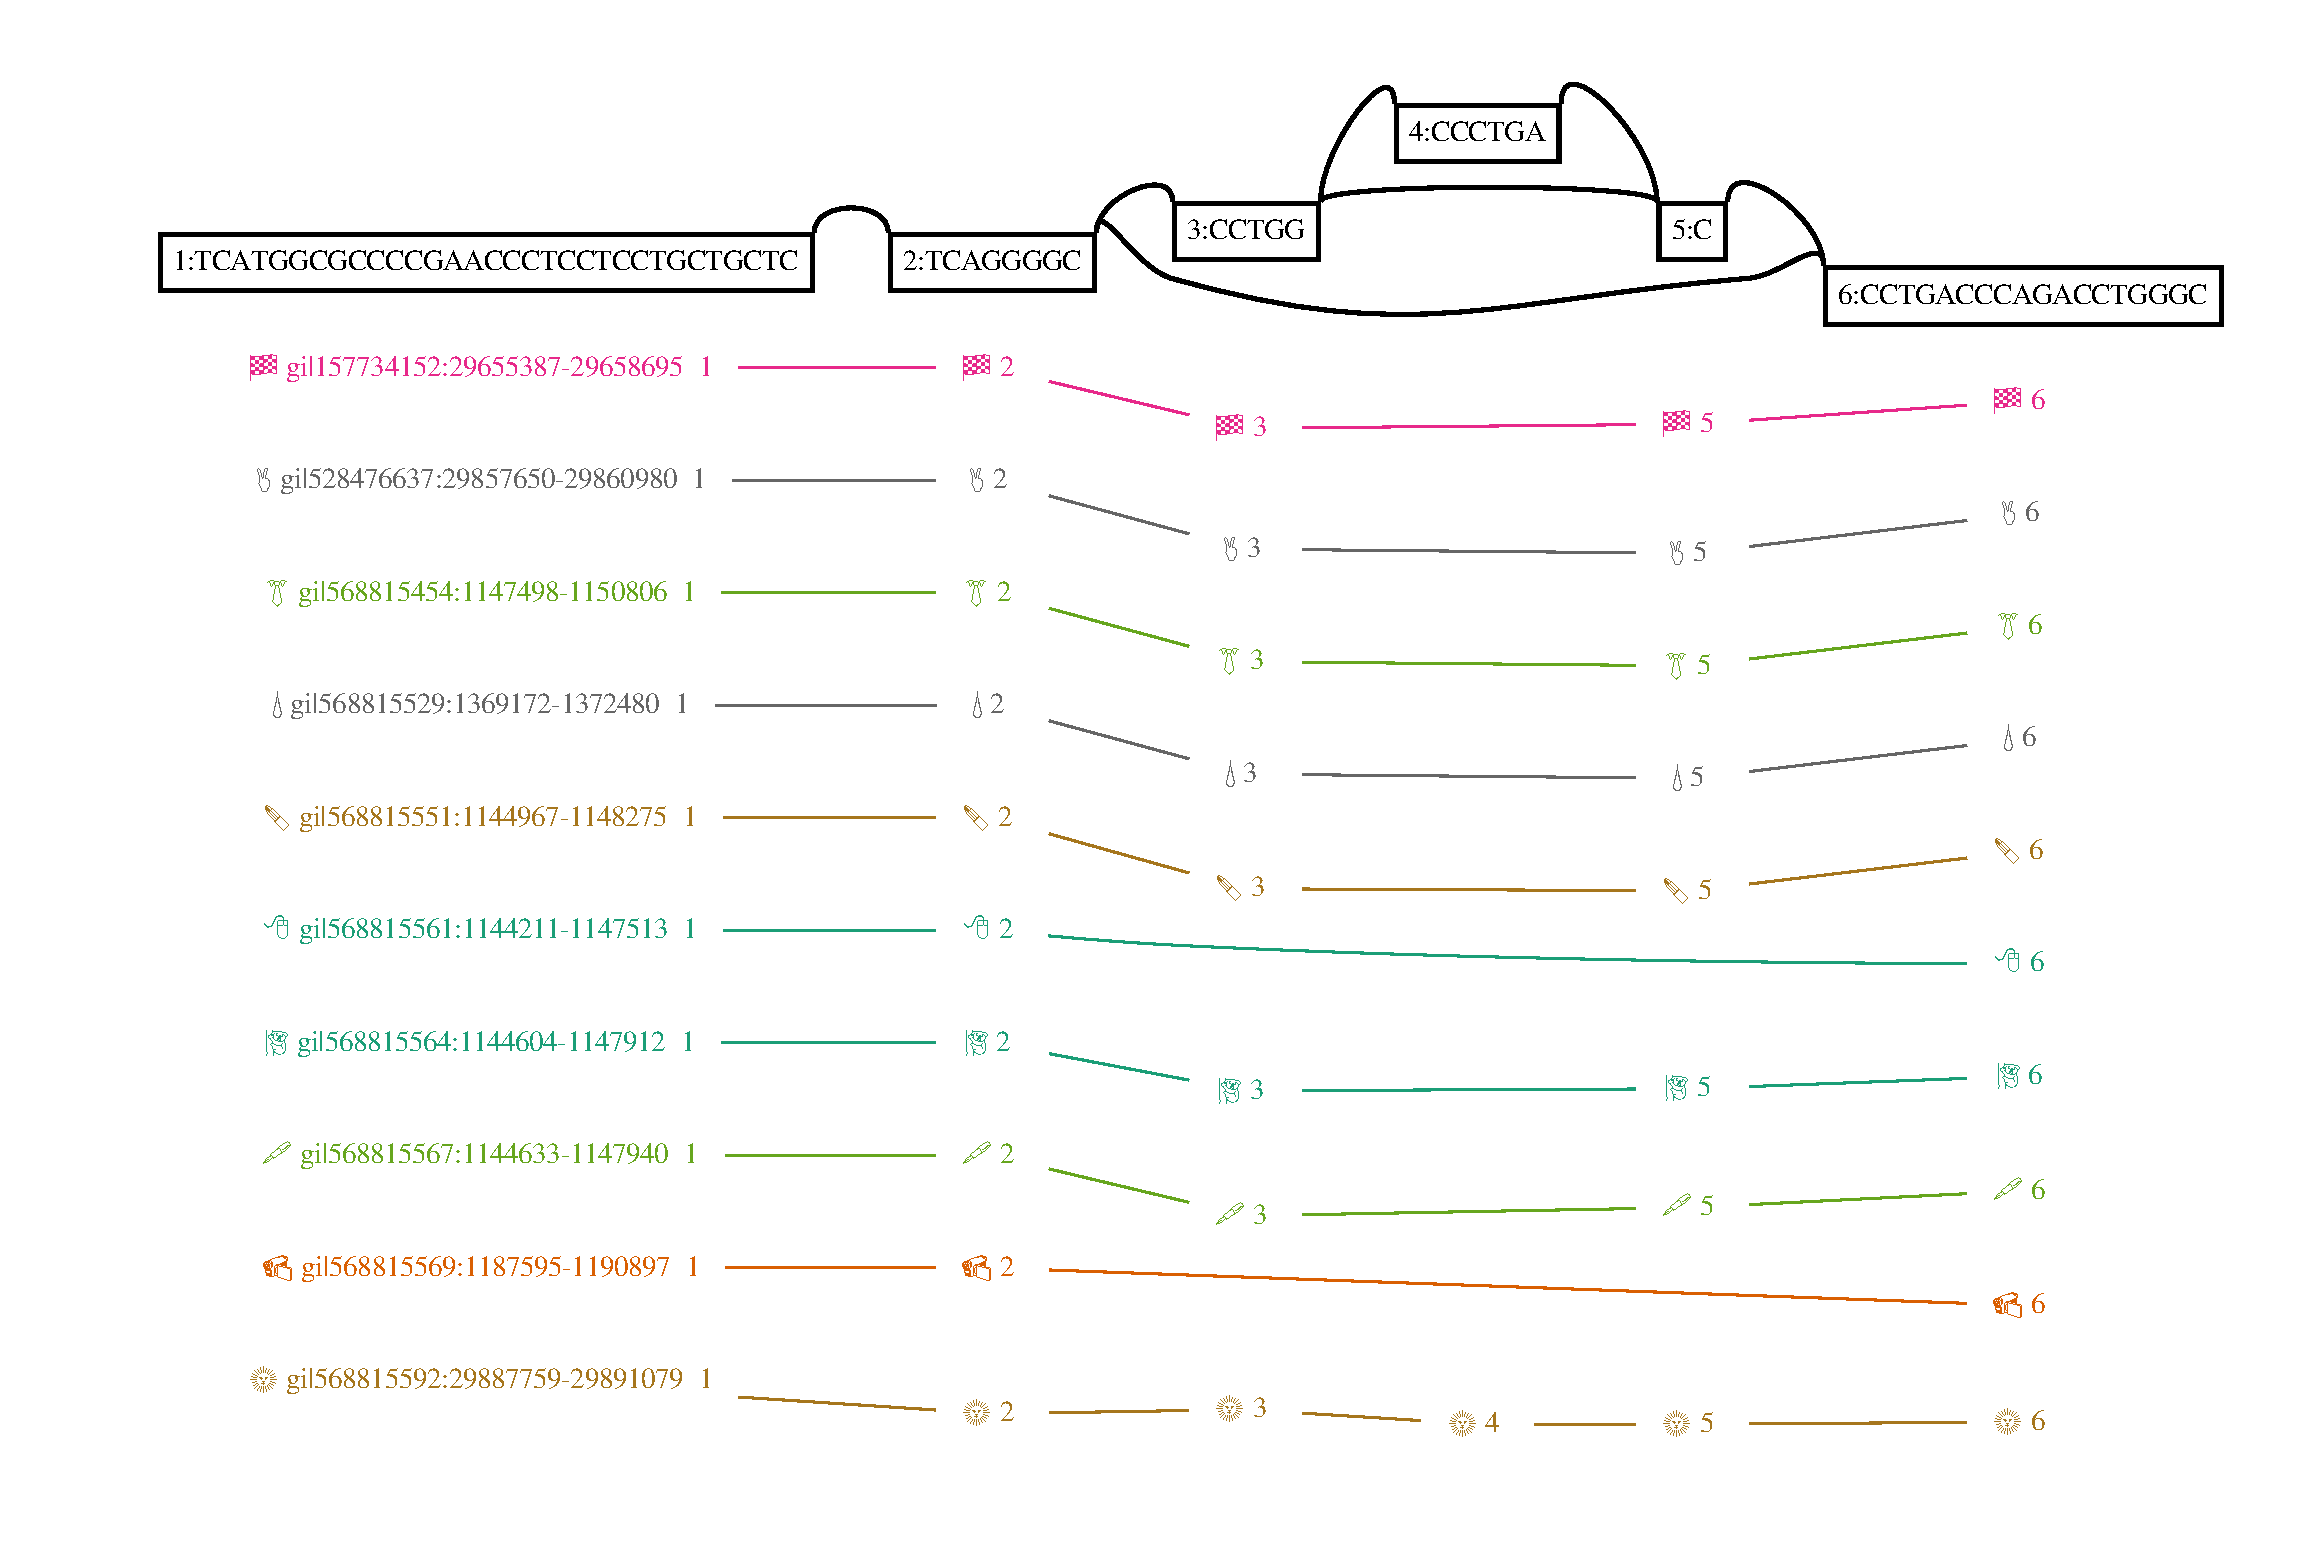
\includegraphics[width=1.0\textwidth]{Chapter2/Figs/vg_view_dp_H-3136_dot.pdf}
\caption[Hierarchical visualization with Graphviz's {\tt dot}]{The beginning of a variation graph built by progressive assembly of the GRCh38 haplotypes in HLA gene H-3136 visualized using {\tt dot}.
  \DIFaddbeginFL \DIFaddFL{The graph topology of nodes and edges is represented above, with node ids and sequences labeled the rectangular nodes, and edges connecting the upper corners of nodes representing the edge topology relative to the forward strand of the graph.
  Below, paths in the graph are represented in a matrix-like format, with each mapping in the path represented by a node id and a colored emoji, and subsequent steps connected by a colored line.
  The emoji/color combination is determined by a hash function applied to the path name.
  A hidden edge connecting each path mapping step and the correpsonding node in the graph topology is used to force the rendering to place them at the same horizontal position, increasingly legibility.
}\DIFaddendFL }
\label{fig:vg_view_dot}
\end{figure}

\subsection{Force directed models}
%*1p 1.5h*

Not all graphs yield easily to hierarchical layout algorithms.
Graphviz also includes a force-directed layout algorithm {\tt neato} that simulates the layout which would occur if connected nodes ``pull'' each other together and non-connected nodes ``repel'' each other apart.
While the same input to {\tt dot} may be used with {\tt neato}, in practice the node labels become impossible to read and the edge types are confusing to infer, so a simplified rendering is produced without specific sequence labels on the nodes.
This can still capture the overall structure of the graph as seen in figure \ref{fig:vg_view_neato}.

\begin{figure}[htbp!] 
\centering    
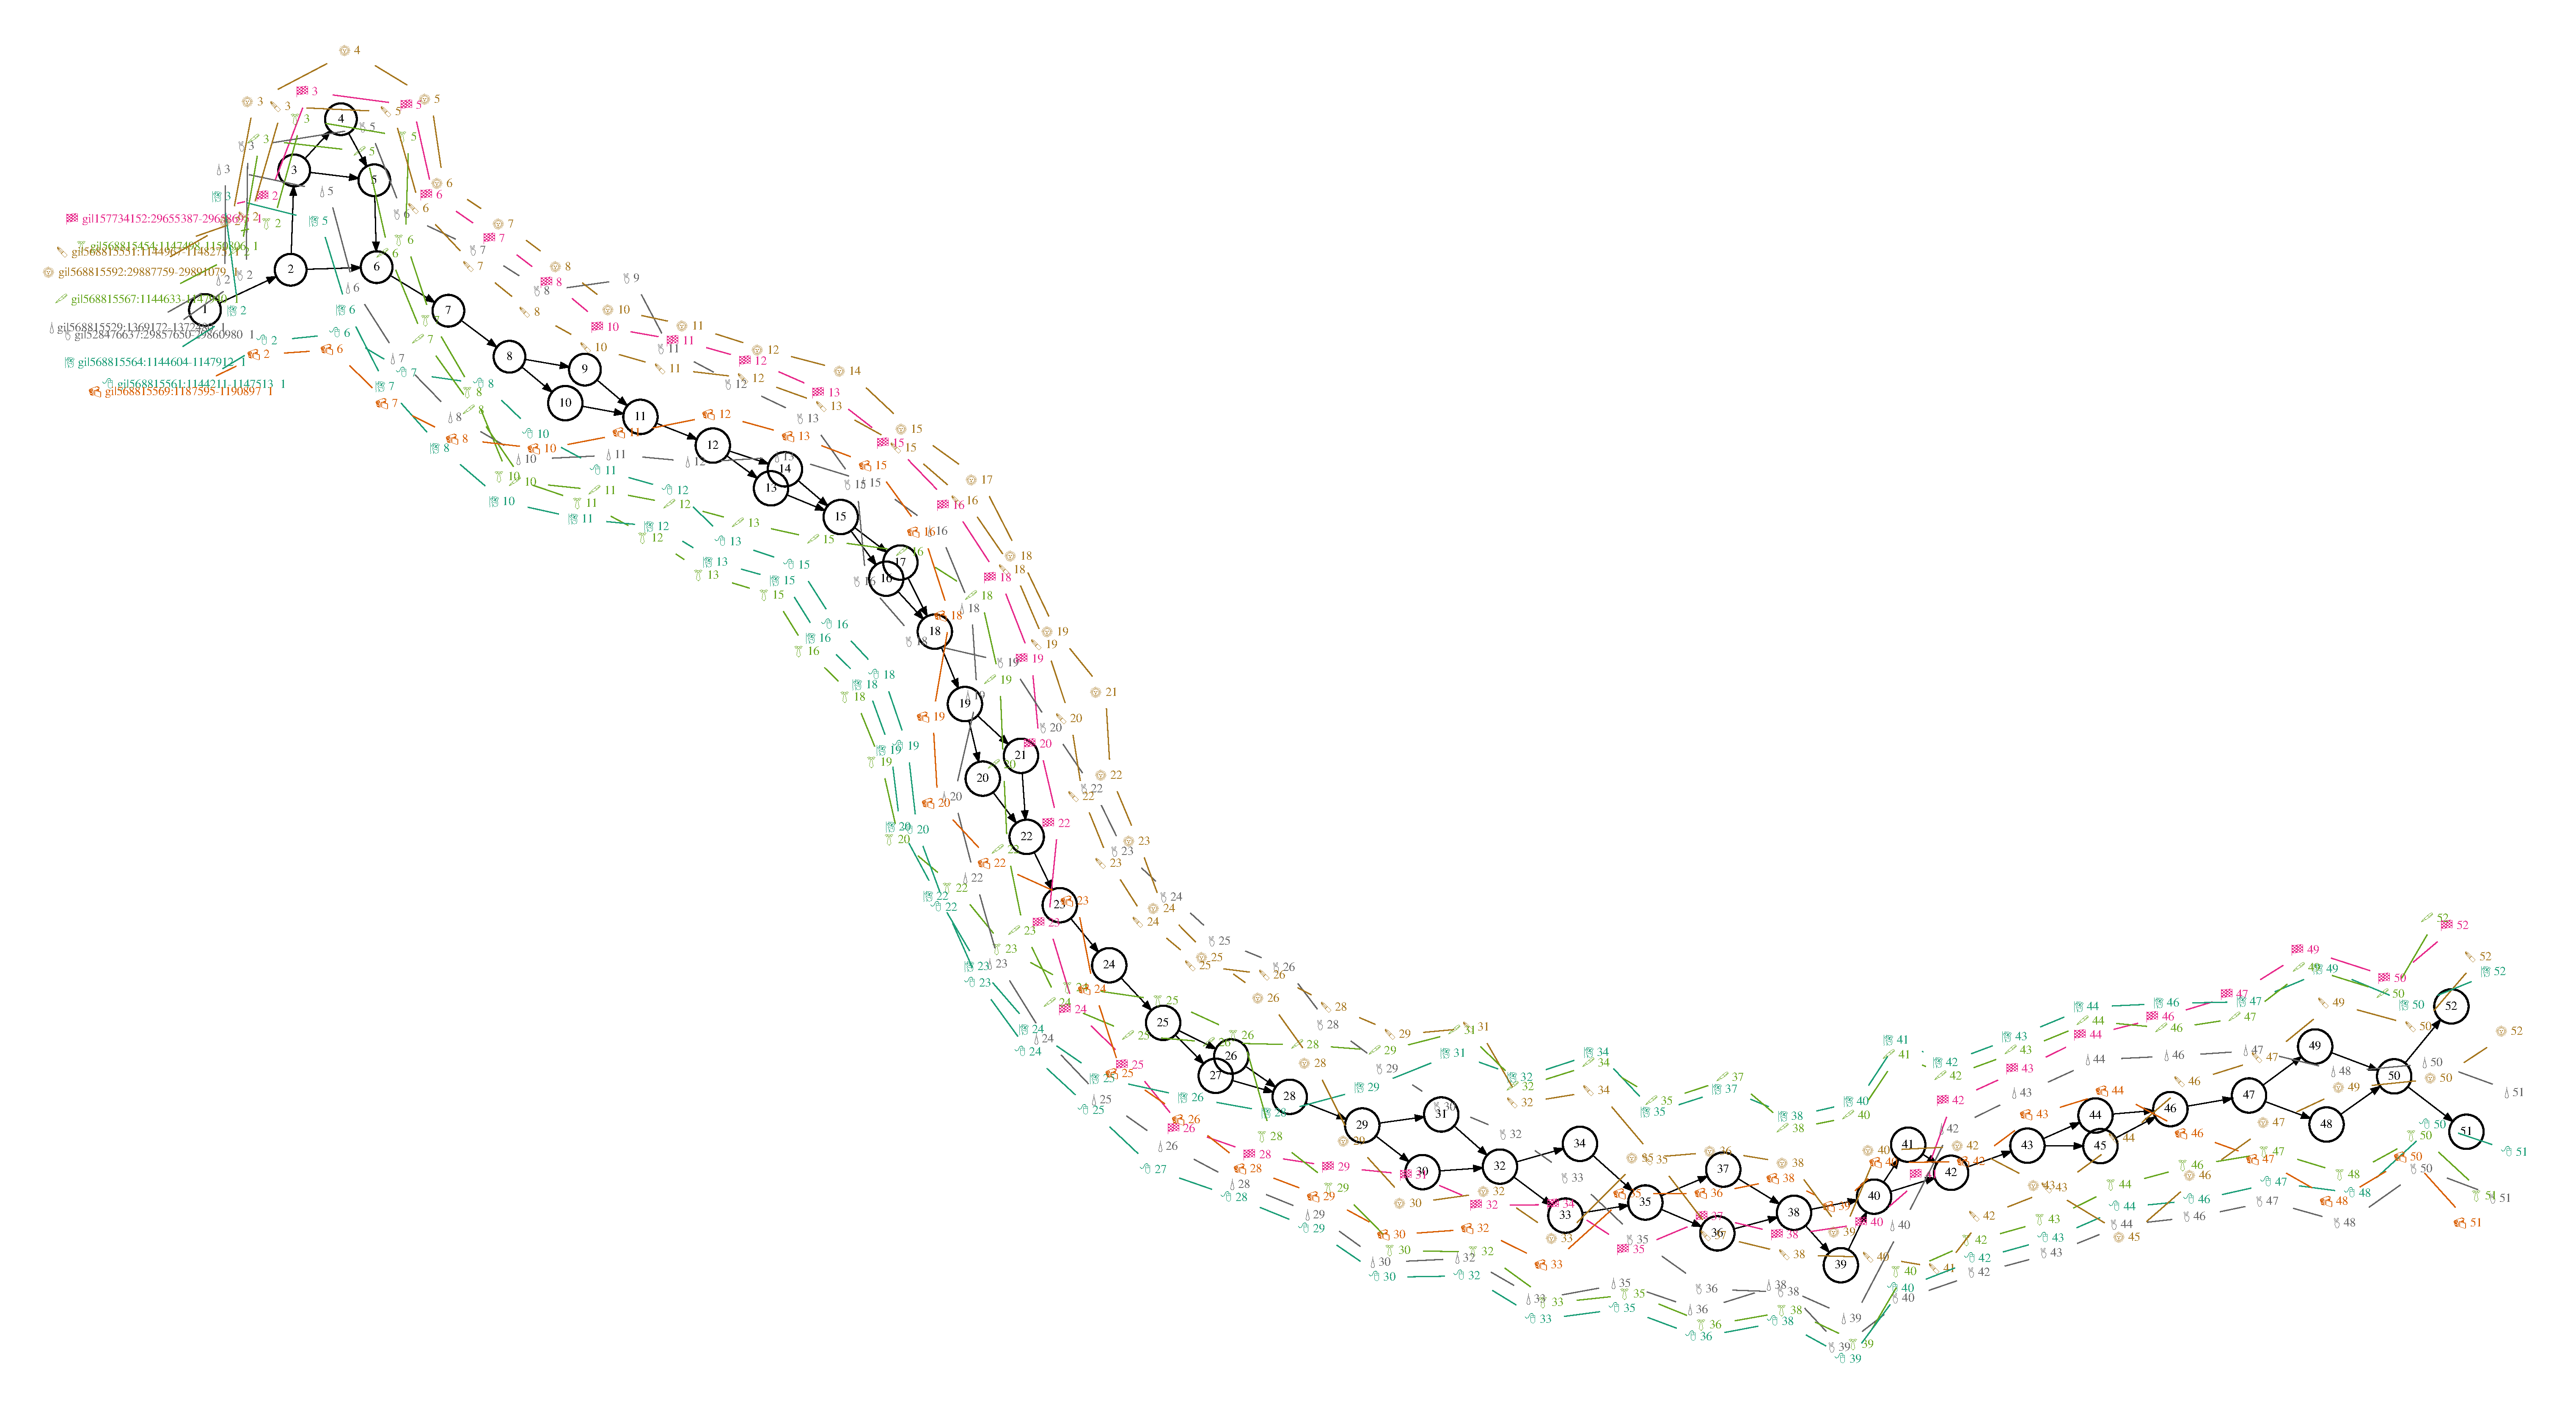
\includegraphics[width=1.0\textwidth]{Chapter2/Figs/vg_view_dpS_H-3136_neato.pdf}
\caption[Force-directed layout with Graphviz's {\tt neato}]{
  A larger region of the same variation graph in figure \ref{fig:vg_view_dot} rendered using {\tt neato\DIFaddbeginFL \DIFaddFL{.}\DIFaddendFL }
    \DIFaddbeginFL \DIFaddFL{Here, each path in the variation graph is represented by a colored path, with the node steps 
    As in \ref{fig:vg_view_dot}, paths in the graph are represented as colored paths connecting node ids and emoji.
    The same hash function is used to determine the color and emoji combination used to label each path.
    Each mapping in each path corresponds to one such node id / emoji label, and it is connected to the previous and subsequent steps by a line of the same color.
    A hidden edge connects each of these path steps to the node it corresponds to.
    This link causes the force directed layout algorithm to draw each each path mapping node close to the node it refers to.
    Note that the graphviz data input here rendered by }{\tt \DIFaddFL{neato}} \DIFaddFL{is the same as that given to }{\tt \DIFaddFL{dot}} \DIFaddFL{in \ref{fig:vg_view_dot}}\DIFaddendFL .
}
\label{fig:vg_view_neato}
\end{figure}

While this rendering captures the path space of the graph even in arbitrary graphs, it cannot scale to graphs of significant size due to its approximately $O(|N|^3)$ scaling.
The largest graphs I have visualized using this method contain tens of kilobases of sequence.
{\tt Bandage} \cite{wick2015bandage} is an alternative method which is oriented towards visualizing assembly graphs.
It reads GFA as input and provides an interactive rendering of the graph topology.
This approach can render graphs of up to tens of megabases.
Figure \ref{fig:vg_view_bandage} shows the properties of this technique using the same region of H-3136.

\begin{figure}[htbp!] 
\centering    
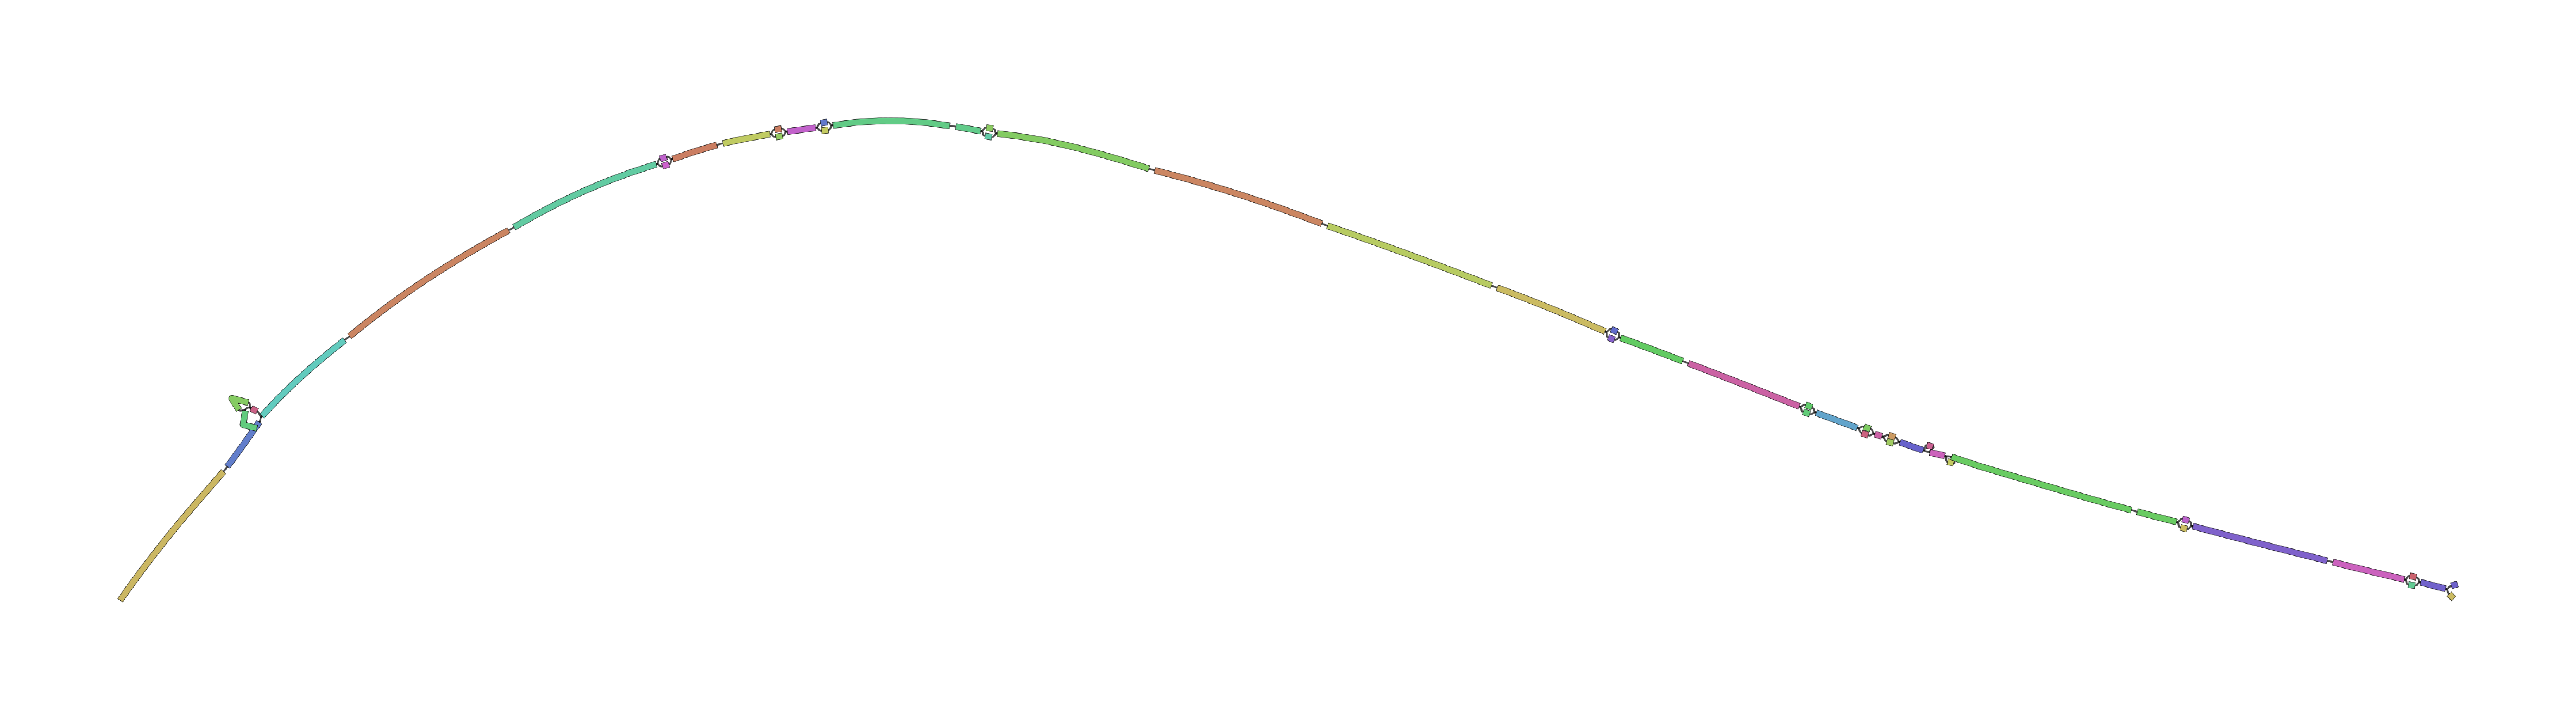
\includegraphics[width=1.0\textwidth]{Chapter2/Figs/vg_view_H-3136_Bandage.pdf}
\caption[Force-directed layout with Bandage]{
  The graph from figure \ref{fig:vg_view_neato} rendered using {\tt Bandage}.
  \DIFaddbeginFL \DIFaddFL{This rendering algorithm does not include the graph's paths.
  Here, node colors have been randomly assigned, and serve to indicate where nodes start and end.
}\DIFaddendFL }
\label{fig:vg_view_bandage}
\end{figure}

\subsection{Linear time visualization}

Graph layout algorithms are computationally complex due to their need to iteratively relate all components of the graph to all others.
In these layouts, we can observe large scale features about the topology and organization of the graph.
These views are helpful in many contexts, but the computational complexity of obtaining them prevents us from quickly visualizing larger graphs.
Also, they do not scale efficiently to large path sets, and it is often difficult to understand alignments or other path-related on the graph using them.

To resolve these issues I developed a linear time rendering algorithm that projects a given VG, as indexed by XG, into a vector graphics format using the widely-available graphics library {\tt libcairo}.
This visualization algorithm uses the sequence basis vector $S_\textbf{iv}$ as a coordinate system to position all elements of the graph.
The graph topology itself is laid out in accordance with the node representation in $S_\textbf{iv}$, flowing from left to right at the top of the rendering.
Node lengths are shown using a black bar, with the sequence labels given below.
The graph topology is rendered above the node set, and layout of these edges can be completed in linear time as they are rendered as simple splines connecting node ends.
Paths, or other annotations such as coverage per read set, are displayed below as colored bars matching the subset of the node space that they cover.
Where paths traverse a given node multiple times, an annotation is added to indicate the copy number.
This technique is implemented as {\tt vg viz}, and an example rendering is given in figure \ref{fig:vg_viz}.

\begin{figure}[htbp!] 
\centering    
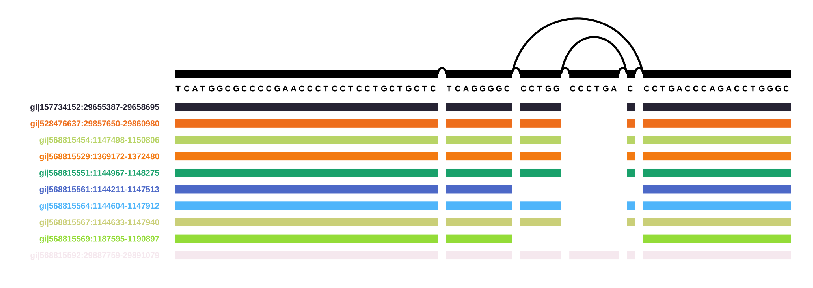
\includegraphics[width=1.0\textwidth]{Chapter2/Figs/vg_viz_H-3136.pdf}
\caption[Linearized variation graph visualization]{
  The same variation graph in figure \ref{fig:vg_view_dot} rendered using {\tt vg viz}.
  \DIFaddbeginFL \DIFaddFL{Above, we see the graph topology in terms of nodes, their lengths, and the edges that link their ends.
  Node sequence labels are shown below this topology, at the nodes they correspond to.
  Below, each path in the graph occupies a single position on the vertical axis.
  A hash function projects each path into a color, although the specific mapping is not the same as in figures \ref{fig:vg_view_dot} and \ref{fig:vg_view_neato}.
  Each horizontal position corresponds to a unique graph position.
  Where a path touches this graph position, we applied a colored bar at the given vertical axis position corresponding to the path.
  This rendering thus represents paths as binary vectors over the sorted sequence space of the graph.
}\DIFaddendFL }
\label{fig:vg_viz}
\end{figure}

It is important to recognize that this approach is lossy.
Path ordering is not clearly represented, as the paths are treated like masks over the sequence space of the graph.
Furthermore, it can be difficult to interpret complex graphs as the topology of the graph is obscured in the simplistic rendering.
{\tt vg viz}'s linear layout treats the graph sequences as a basis space in which other paths or alignments may be interpreted.
This simplistic view is central to many potential applications of {\tt vg}, which I further discuss in section \ref{sec:basis_space}.
The linear scaling of the algorithm should allow it to be applied to whole genomes, provided suitable front-end visualization software can be built, such as in a web interface.

\section{Graph mutating algorithms}

To use variation graphs as reference systems, we need to be able to modify them.
Algorithms in graph theory are frequently based on graph transformations, and I have discussed some of them in the context of assembly and whole genome alignment.
{\tt vg} implements many algorithms that alter the graph, but a number are of importance to its development as a system for resequencing, and I detail them here.

\subsection{Edit}

As discussed in section \ref{sec:extending}, the extension of a variation graph to include new sequences and paths can be thought of as a transformation yielding a bijection between the new and old graphs $edit(G, A) \to (G', \Phi)$.
The main issue which adds complexity to this process is that nodes represent more than a single character.

If nodes did represent a single character, then they would remain atomic through graph extension.
It is simple to edit a ``basepair'' graph of this type: $G = (N, E, P)$, where $\forall_{n \in N}{|seq(n)| = 1}$.
We walk through the alignments to it $A = a_1\ldots a_{|A|}$, adding novel bases represented in them ($seq(A) \notin G = N_A$) as new nodes.
Then for each alignment $a_i$, we add edges connecting nodes in the order they would be traversed by the path of the alignment embedded in the graph $p_{a_i} \in G'$, yielding $E_A$.
Finally, we add paths representing the embedded alignments $P_A$.
The resulting graph unifies these additions $G' = (N \cup N_A, E \cup E_A, P \cup P_A)$.

To achieve lower representation costs in graphs with sparse variation, we usually compress the graph so that nodes cover multiple bases and thus we must consider the editing process in multiple phases.
We first modify graph $G$ so that every novel sequence will be added at the start or end of a node.
We do this by breaking nodes into multiple derivative nodes when they overlap mappings that do not match the graph using $break(G, A) \to (G', \Phi)$.
For instance, if $seq(n_i) = {\tt GATTACA}$ and we have a SNP ${\tt T} \to {\tt C}$ at offset 4, we would obtain $n_i \to n_i', n_i'', n_i''' : seq(n_i') = {\tt GAT} $, $seq(n_i'') = {\tt T}$, $seq(n_i'') = {\tt ACA}$.
We can then apply $translate(A, \Phi) \to A'$, and add edges to $G'$ implied by the alignments as we would when editing a graph with single character nodes.

\subsection{Pruning}
%*2.5p 3h*

The number of paths in a sequence graph grows exponentially with the number of variable sites.
As I have discussed, this causes problems for alignment algorithms and graph sequence indexing.
While we can use efficient disk-backed index construction algorithms like GCSA2 to mitigate the effects of this exponential scaling, only a handful of dense clusters of variation in the graph can increase the memory requirements of path enumeration beyond any reasonable level.
To control this we restructure the graph to limit recombinations in the global sequence index.

We have explored two main techniques for the reduction of graph complexity.
In the first, we prune regions of the graph which have high path complexity using a depth-first search (DFS).
We can optionally add back known haplotypes, in order to mitigate the loss of information from the index.
For VCF-based VGs, where we have haplotype panels, the performance of local alignment is unaffected by the topological complexity, so we only need to apply this pruning to the graph input to GCSA2 indexing.
In assembly graphs, we find that nodes which represent repeats can sometimes have extremely high degree, which causes problems both for indexing and local alignment to the graph.
There, we must remove these nodes in order to use the graph even for local alignment.

\subsubsection{\emph{k}-mer \emph{m}-edge crossing complexity reduction}

In $k$-mer complexity reduction, we enumerate the $k$-mers of the graph, removing edges when a given $k$-mer crossing them would cross $> m$ edges.
We implement this filter, $prune(G, k, m) \to G_\textbf{simple}$, using the $k$-mer enumeration algorithm that generates a DBG from the variation graph, only that our walks through the graph are bounded at $m$ edge crossings.
For each offset in each node $n_i$ and $\overline{n_i}$, we run a DFS forward until we have read $k$ characters of the graph.
During the pruning operation, instead of emitting the $k$-mers with their contexts, we stop the DFS when we have crossed $m$ edges.
We record the edge in $E_\textbf{complex}$. % = \{ e_{ij} : \exists p \in G : |p| > m \mbox{, } node(p_{|p|-1} = i) \mbox{, } node(p_{|p|}) = j \}$.
We thus derive the subgraph from the current graph by removing the complexity-inducing edges: $(N, E \setminus E_\textbf{complex}, P) \to G_\textbf{simple}$.
It can be helpful to remove any small isolated components that result from this pruning, which can be done with a linear subgraph enumeration algorithm and the measurement of the sequence length of each.
A disjoint component $G_\textbf{sub} \in G_\textbf{simple} : \forall_{e_{ij} \in N_\textbf{sub}} n_i \in N_\textbf{sub} \land n_j \in N_\textbf{sub}$ must have length $\sum_{\forall n \in N_\textbf{sub}} |seq(n)| \geq {\cal J}$.
By default, we use $k=24$, $m=3$, and ${\cal J}=33$.

\subsubsection{Filling gaps with haplotypes}

Although removing complex regions will reduce the number of recombinant haplotypes represented by the graph, it is likely to also remove sections of known haplotypes.
We can retain the complexity reduction without losing sequences in known haplotypes by replacing the pruned regions in $G_\textbf{simple}$ with unfolded copies of each haplotype sequence.
When we have a single reference path in $G_\textbf{ref}$, we can accomplish this by overlaying $G_\textbf{simple}$ and $G_\textbf{ref}$.
However, this will not achieve the desired result with even two overlapping paths, as where these differ they would reintroduce the re-combinatorial explosion that we hope to resolve with pruning.
An alternative is to copy the haplotypes in the GBWT index that stretch from one border to the other of each removed region into the removed subgraphs in $G_\textbf{simple}$.
Doing so, we must preserve a mapping between the new nodes and the previous underlying ones in $G$.
This allows matches to the haplotypes to be converted into matches in the base graph.
The exact method by which this filling implemented is described in \cite{siren2018haplotype}.

\subsubsection{High degree filter}

Because they separate dense variation into heterozygous bubbles, assembly graphs may feature greater ``smoothness'' than VCF-based graphs locally.
But, in the context of repeats, they can contain nodes with exceptionally high degree.
If these cluster together then they generate highly-connected regions that introduce degeneracy in the path space of the graph, and cause problems for $k$-mer enumeration and GCSA2 indexing.
Furthermore, the local alignment methods in VG do not support efficient alignment through such dense regions.
Preventing this is relatively simple, in that we remove nodes with more than ${\cal D}$ edges linking them to the graph, yielding $G_\textbf{prune} : \forall_{n_i \in N_\textbf{prune}}{{\cal D} \geq |\{ e_{*i} \cup e_{i*} \cup e_{\overline{i}*} \cup e_{*\overline{i}} \}|}$.

It is not necessary that our local alignment suffers from high-degree nodes.
The problem is that GSSW is provided an alignable graph that is an extracted subset of the full graph.
If this subgraph is extracted using context expansion in the graph, then high-degree nodes will generate extremely large subgraphs.
One solution would be to use the bit-parallel string to graph alignment approach in \cite{rautiainen2018bit}, as this achieves optimal bounds in the size of transformed graph to which we align.
Alternatively, the graph exploration should be more directly linked to the alignment process.
The X-drop aligner {\tt dozeu} could be adapted to this approach, as the X-drop parameter would provide a natural limit to the graph exploration.
Such approaches may allow us to tolerate a larger ${\cal D}$, but it seems unlikely that they will allow alignment to be driven through the most-tangled areas of the graph without a large performance penalty relative to graphs with lower maximum degree.

\subsection{Graph sorting}
%*1p 1h*

To achieve as much partial ordering as possible, we order and orient the nodes in the graph using a topological sort.
The sort is guaranteed to be machine-independent given the initial graph's node and edge ordering.
The algorithm is well-defined on non-DAG graphs, but in these cases the order is necessarily not a topological order.
Our approach is a bidirected adaptation of Kahn's topological sort \cite{kahn1962topological}, which is extended to handle graph components with no heads or tails.
This algorithm can be understood as a kind of seeded depth first search through the graph.
Where the graph has nodes which are pure heads, it begins there.
Otherwise, a set of seed nodes which are stably selected given a particular graph are used to begin the sort.
The details of this procedure are provided in algorithm \ref{alg:pseudotoposort}.

Sorting can provide a simple optimization during read alignment.
If the reference graph has been sorted, then we can use the given order to generate node identifiers, embedding the rank of each node in its id.
We can detect if a given subgraph is possibly non-acyclic if $\exists e_{ij} \in E : i > j$, and if so submit the graph to sorting, unfolding, and DAGification before applying local alignment.

Similarly, the sort allows us to project data in the context of the graph into a single dimension.
Provided the graph is regionally partially ordered, this projection preserves local structures, which is a desirable property.
This makes the sort applicable to visualization techniques as in figure \ref{fig:vg_viz}.

\begin{algorithm}
  \caption[Pseudo-topological sort]{Pseudo-topological sort}
  \label{alg:pseudotoposort}
  \begin{algorithmic}
    \State $G = (N, E, P)$
    \Comment{A copy of our input graph which we will destructively modify}
    \State $L \gets [ \ldots ]$
    \Comment{Stores the pseudo-topological order}
    \State $S \gets \emptyset$
    \Comment{Set of nodes which have been oriented but not yet traversed}
    \State $V \gets \{ n_i \} \in N : \not \exists e_{ji} \forall n_j \in N$
    \Comment{We start from the head nodes of the graph}
    \If{$V = \emptyset$}
    \Comment{If there are no head nodes, we use ``seed'' nodes}
    \State $V \gets \text{Stably-selected seed nodes} \in N$
    \EndIf
    \While{$V \neq \emptyset$}
      \State $n \gets n \in V$
      \Comment{Select a seed node}
      \State $V \gets V \setminus \{n\}$
      \Comment{Remove it from the input node set $V$}
      \State $S \gets S \cup \{n\}$
      \Comment{Store it in our working set $S$}
      \While{$S \neq \emptyset$}
        \State $n_i \gets n_i \in S$
        \Comment{Remove an oriented node from $S$}
        \State $S \gets S \setminus \{n_i\}$
        \State $L \gets [L[1] \ldots L[|L|], n_i]$
        \Comment{Append it to our output order $L$}
        \For{$\forall n_j : e_{ij} \in E$}
          \State $E \gets E \setminus \{e_{ij}\}$
          \Comment{Remove the edge from our edge set}
          \If{$\not \exists e_{kj} \forall k \in N$}
          \Comment{$n_j$ has no other edges to that side}
          \If{$e_{i\overline{j}}$}
            \State $n_j \gets \overline{n_j}$
            \Comment{Orient $n_j$ so the side the edge comes to is first}
          \EndIf
          \State $N \gets N \setminus \{ n_j \}$
          \Comment{Remove $n_j$ from $N$}
          \State $S \gets S \cup \{ n_j \}$
          \Comment{Insert $n_j$ into $S$}
          \Else
          \Comment{This helps start at natural entry points to cycles}
            \State $V \gets V \cup \{ n_j \}$
            \Comment{Record $n_j$ as a place to start when $S$ is empty}
          \EndIf
        \EndFor
      \EndWhile
    \EndWhile \\
  \Return{$L$} \Comment{Return our pseudo-topologically sorted order and orientation}
\end{algorithmic}
\end{algorithm}


\subsection{Graph simplification}

Assembly algorithms often employ a \emph{bubble popping} phase, in which small bubbles, which are graph components connected to the rest of the graph through a single source and sink node, are replaced by linear components representing the most-likely path through the bubble given the read data.
In {\tt vg} we can carry out a similar operation based on the bubble decomposition of the graph.
Unlike assembly graph bubble popping, we must retain information about the embedded paths and annotations in the variation graph.
Simplification has a number of potential applications, for instance in reducing the complexity of visualizations of large variation graphs.

\section{Graphs as basis spaces for sequence data}
\label{sec:basis_space}

If we can construct a graph which embeds all the sequences of all genomes which we are interested in, we resolves the separation between reference sequence and variation that is present in standard resequencing.
This suggests that the intermediate steps in resequencing may be made redundant.
If variation is already available during alignment then there is no need for a variant detection phase.
However, if the graph does not include variation in our samples, then variant calling is required.
In {\tt vg} we have implemented several methods to do so.
Similarly, we have implemented coverage summaries of read sets that may be used directly in downstream analyses.

\subsection{Coverage maps}

Numerous population genetic analyses are based on matrix representations of a collection of genomes.
Such models can be used to infer population structure and phylogeny, as well as to associate phenotypes to genomic variants.
If the variation graph used as a reference contains all sequences relevant to our analysis, then a matrix of per-base coverage of the graph by sample will provide highly representative information to downstream analyses.
Exceptions include structural variation that does not result in coverage changes, such as balanced events like inversions.
Also, some local patterns of variation between successive small variation will not be distinguishable.
If we were to annotate edges with their coverage, this method would produce a result equivalent in information content to a Markov model.
It is thus clear that any coverage based index will be lossy relative to the full read set.
However, the lossiness reduces the information cost of storing and processing these coverage maps.
As I described in section \ref{sec:coverage_index}, in {\tt vg} I developed an efficient method to accumulate coverage information of this kind across the graph.

\subsection{Bubbles}

In a sequence graph, a \emph{bubble} is a pair of paths which start and end at the same nodes ($s$, $t$) but are otherwise disjoint in the graph \cite{zerbino2008velvet}.
Bubbles encompass our intuition about genetic variation in graphs.
A homologous sequence corresponding to the common start and end nodes in the bubble flanks two or more alternative alleles in the middle.
These structures were first considered in the context of finding small variation, and it was only in recent years that methods were developed to efficiently enumerate all bubbles of any size in DAGs \cite{birmele2012efficient}.

Bubbles can nest and contain more complicated internal structures between the paths through them.
The bubble may be generalized to the idea of a \emph{superbubble}, which is a directed, acyclic component of a graph with a single head and tail node \cite{onodera2013detecting}.
As for bubbles, efficient enumeration of superbubbles is possible in a DAG \cite{brankovic2016linear}.
The optimal method relies on a recursive topological sort of the graph to structure the nested bubbles.
Candidate node starts ($s$) and ends ($t$) are found following the definition of a superbubble.
The set of candidates is then validated by range min queries (RMQ) to produce the set of superbubbles.
As sort is linear $O(|N| + |E|)$, and the candidate enumeration and RMQ may be implemented on the sorted graph in $O(1)$ each, this yields a linear time algorithm for the enumeration of superbubbles.

The DAG requirement of this method is a significant limitation.
In order to apply the superbubble enumeration to an arbitrary graph we must first DAGify it.
In response, I worked with Benedict Paten and others to generalize the idea of a genetic site to support arbitrary bidirectional sequence graphs \cite{paten2018superbubbles}.
To formulate a generalization of superbubbles, we introduce the concept of a \emph{snarl}, which is any graph component connected to the rest of the graph by two or fewer bordering nodes\footnote{In the paper the formulation is based on a bi-edged graph akin to the Enredo graph, but we note that a node-based formulation is equivalent and matches the other models in this section.}.
Snarls whose internal separated component is acyclic and does not contain any tips are \emph{ultrabubbles}.

Paten observed that trees embedded in the Cactus graph transformation of a variation graph corresponded to the standard concept of superbubbles.
Specifically, the cactus graph is transformed into a \emph{cactus tree} in which each simple cycle in the cactus graph becomes a special kind of node.
Various rootings of this tree may then be used to define a hierarchy of bubbles.
The bidirectional nature of the variation graph mean that snarls can embed each other in a manner akin to how the twist used to generate an M\"{o}bius strip results in it having a single surface and border.
In these cases the resulting cactus tree will support multiple alternative ultrabubble tree rootings, and so unlike the bubble and superbubble decompositions for DAGs the ultrabubble decomposition is not unique.
We can enumerate a subset of these by identifying bridge edges (typically representing tips) in the ``bridge forest'', which is the result of a contraction of the cycles in the cactus graph into a set of top-level cycle representing nodes, and then use them to produce various rootings of the cactus tree.

Ultrabubbles and superbubbles provide a natural framework in which to reason about the hierarchy of variable genetic sites embedded in a graph.
As such they provide the basis for generic models of genotype inference based on variation graphs which are capable of genotyping any kind of genetic variation, including structural variation as well as nested variation, in the same model as SNPs and indels.

\subsection{Variant calling and genotyping}

Given a definition of variable genetic loci in the graph, we can build a genotyping system capable of generating genotype calls in the context of the graph.
In {\tt vg} we have explored two such methods.
The first, originally implemented in {\tt vg call}, generalizes the concepts first implemented in {\tt samtools mpileup} to work on the graph.
A set of alignments are first reduced to pointwise edits against the graph and per base coverage of the graph.
This graph ``pileup'' is then processed by a genotyping algorithm that considers genetic sites using the ultrabubble model.
A schematic overview of the method is shown in figure \ref{fig:vg_call}.

\begin{figure}[htbp!]
  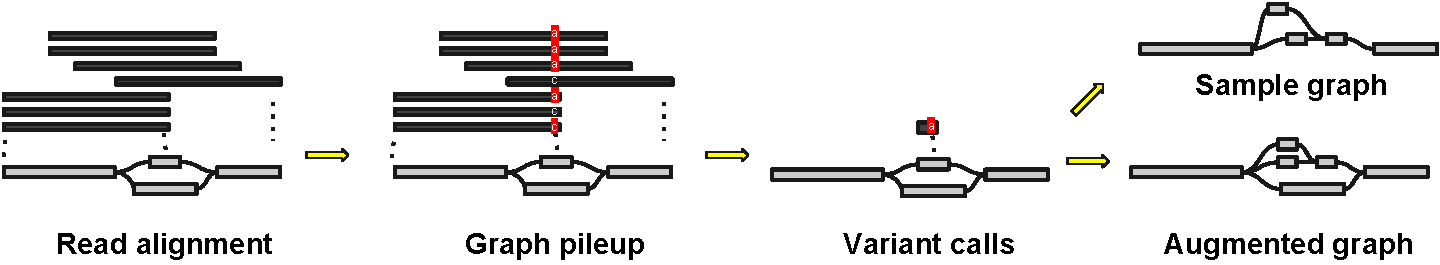
\includegraphics[width=1.0\textwidth]{Chapter2/Figs/vg_call.pdf}
  \caption{
    Pileup variant calling with {\tt vg call}
    }
  \label{fig:vg_call}
\end{figure}

The second model, implemented in {\tt vg genotype}, embeds the alignments in the variation graph using $edit(A, G_\textbf{base}) \to (G_\textbf{aug}, \Phi_{\textbf{aug}\to\textbf{base}})$, and then genotypes across the ultrabubbles of $G_\textbf{aug}$ which are supported by reference paths in $G_\textbf{base}$ or reads.
As the resulting genotypes are represented as unordered sets of paths in $G_\textbf{aug}$, they are projected back into the coordinate space of $G_\textbf{base}$ using the translation $\Phi_{\textbf{aug}\to\textbf{base}}$.
An overview of the process is shown in figure \ref{fig:vg_genotype}.

\begin{figure}[htbp!]
  \centering
  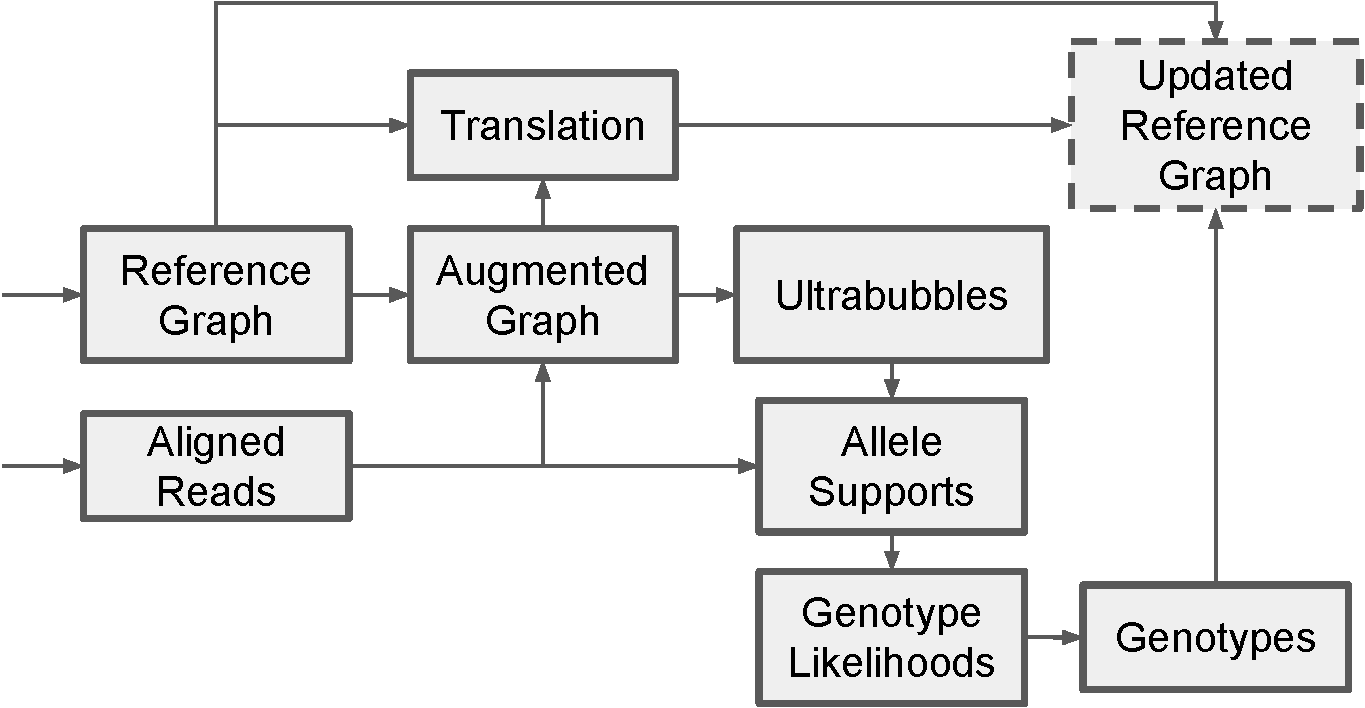
\includegraphics[width=0.7\textwidth]{Chapter2/Figs/vg_genotype.pdf}
  \caption{
    Graph augmentation-based variant calling in {\tt vg genotype}
    }
  \label{fig:vg_genotype}.
\end{figure}

While principled, the full augmentation model in {\tt vg genotype} is very expensive to compute.
The pileup model has proven to be more efficient.
Over time {\tt vg call} has been adjusted to implement some features of the full graph augmentation model in {\tt vg genotype} where the graph is augmented only with sequences supported by some number of alignments at a given quality threshold.
Both methods employ a diploid specification of the genotyping model in freebayes \cite{garrison2012haplotype} to develop their posterior estimates of variant quality.
The generalization of SNP and indel calling to haplotype calling implemented in freebayes corresponds to the same allele model used in both {\tt vg} variant calling methods.
Alleles correspond to DNA sequences of arbitrary length, anchored at the ends to the reference genome (in the case of freebayes) or to the rest of the graph (as in the ultrabubbles used in {\tt vg}).

The complexity of running and evaluating genotyping in the graph has slowed development of these methods.
Currently they are still outperformed by standard variant calling methods based on the linear reference, as indicated by our results in the PrecisionFDA variant calling challenge that I will describe in the next chapter.

%\subsection{MEM matching to the bidirectional GBWT}

%\section{Contributions to related computational methods}

% in this chapter I've described things that I've done
% as a consequence of being in this work, here are things that I helped other people to build
% list papers, give references

% gpBWT
% GCSA2
% ...

%%!TEX root = ../thesis.tex
%*******************************************************************************
%****************************** Third Chapter **********************************
%*******************************************************************************
\chapter{Applications}

% **************************** Define Graphics Path **************************
\ifpdf
    \graphicspath{{Chapter3/Figs/Raster/}{Chapter3/Figs/PDF/}{Chapter3/Figs/}}
\else
    \graphicspath{{Chapter3/Figs/Vector/}{Chapter3/Figs/}}
\fi

%*0.5p 1h*

\section{Yeast}
%*0.5p 0.5h*

\subsection{A SNP-based SGRP2 graph}
%*1p 1h*

\subsection{Cactus progressive assembly}
%*0.5p 0.5h*

\subsection{Constructing and comparing variation graphs from whole genome assemblies}
%*3p 2.5h*


\section{Human}
%*0.5p 0.5h*

\subsection{1000GP graph construction and indexing}
%*3p 3h*

\subsection{Simulations based on phased HG002}
%*2p 2.5h*

\subsection{Whole genome variant calling experiments}
%*1p 2h*

\subsection{HGSVC from VCF and progressive alignment of human chromosomes}
%*2.5p 5h*

\subsection{CHiP-Seq}
%*1p 1h*


\section{Ancient DNA}
%*0.5p 0.5h*

\subsection{Simulations with human origins panel}
%*1p 2h*

\subsection{Using 1000GP graph for samples from Martiniano et al 2016}
%*2p 4h*

\subsection{Evaluation of a high-coverage Botai sample}
%*2p 4h*


\section{Neoclassical bacterial pangenomics}
%*0.5p 0.5h*

\subsection{E. coli pangenome from illumina reads}
%*2p 4h*

\subsubsection{Evaluating the core and accessory pangenome}
%*2p 4h*


\section{Metagenomics}
%*0.5p 0.5h*

\subsection{Arctic viral metagenome}
%*2p 1.5h*

\subsection{Human gut microbiome}
%*2p 8h*


\section{RNAseq}
%*0.5p 0.5h*

\subsection{Yeast}
%*1p 2h*

\subsection{C. elegans}
%*2p 5h*

\subsection{Human}
%*2p 12h*


%!TEX root = ../thesis.tex
%*******************************************************************************
%****************************** Third Chapter **********************************
%*******************************************************************************
\chapter{Applications}
\DIFaddbegin \label{chapter:applications}
\DIFaddend 

% **************************** Define Graphics Path **************************
\ifpdf
    \graphicspath{{Chapter3/Figs/Raster/}{Chapter3/Figs/PDF/}{Chapter3/Figs/}}
\else
    \graphicspath{{Chapter3/Figs/Vector/}{Chapter3/Figs/}}
\fi

In the first two chapters I have provided an overview of the theoretical basis of my work and placed it within the history of related approaches.
Here, I will demonstrate how the methods I develop can aid biological insight in a number of species domains.
To do so, I will use methods described in chapter 2 as implemented in {\tt vg}.

The small genome of \emph{Saccharomyces cerevisiae} and ready availability of sources for pangenomic data models made it very useful to my development of {\tt vg}.
I begin by illustrating this for a variety of pangenome constructions and also a variety of read lengths.

However, much interest in bioinformatics is with larger genomes, specifically human.
I use evaluations based on the human genome to validate the ability of {\tt vg} to scale to large genomes.
Through simulation and the analysis of real genomes, I show that the aligner I implement, {\tt vg map}, yields the same quality of alignment as {\tt bwa mem} against linear genomes.
Although {\tt vg map}'s runtime is between five to ten-fold slower than {\tt bwa mem}, it provides improved, less biased alignment against variation graphs.
I develop a variation graph for the reference-guided genome assemblies from the HGSVC project and demonstrate the strong effect of reference bias in ChIP-seq data.

One context where reference bias has very significant effects is in the analysis of ancient DNA (aDNA).
Here short reads and high intrinsic error rates encourage a high rate of reference bias.
I show that alignment against a pangenome graph ameliorates this issue.

{\tt vg} can be applied to any kind of variation graph.
To demonstrate the utility of this, I use de Bruijn assemblers to generate reference variation graphs from collections of raw sequencing reads in the absence of a prior reference.
I recreate a classical pangenomic analysis of core and accessory pangenome by analyzing the coverage of alignments mapped to an assembly graph built from 10 \emph{Escheria coli} strains.
To illustrate the application of \DIFdelbegin \DIFdel{vg }\DIFdelend \DIFaddbegin {\tt \DIFadd{vg}} \DIFaddend to metagenomic data containing unknown source genomes, I show that {\tt vg} enables the full length alignment of reads to a complex assembly graph built from an arctic viral metagenome, and similarly improves alignment to an assembly graph built from a human gut microbiome.
Finally, I demonstrate that the data models and indexes in {\tt vg} are capable of encoding splicing graphs, and that aligning to these splicing graphs allows the direct observation of the transcriptome.

\section{Yeast}
%*0.5p 0.5h*

\emph{Saccharomyces cerevisiae}, commonly known as baker's or brewer's yeast due to its gastronomic applications, has long been among the most important model organisms in biology, and its small genome attracted some of the first population scale whole genome surveys of variation to be undertaken using low-cost sequencing.
The genome of \emph{S. cerevisiae} was the first eukaryotic genome sequenced, in 1996 \cite{goffeau1996life}.
Resequencing studies followed that used \emph{cerevisiae} as a model system to understand genome evolution.
The Saccharomyces Genome Resequencing Project (SGRP) \cite{liti2009population}, which used low-coverage capillary Sanger sequencing to generate a population survey for \emph{cerevisiae} can be seen as a precursor to the 1000GP, in its use of low-coverage sequencing and imputation to establish the panel\footnote{\url{https://www.sanger.ac.uk/research/projects/genomeinformatics/assets/sgrp_manual.pdf}}.
A followup project, the SGRP2, used resequencing and whole genome assembly of high coverage, low cost Illumina sequencing to establish that the greater phenotypic diversity in \emph{S. cerevisiae} relative to its wild relative \emph{S. paradoxus} is likely due to structural variation (as measured by presence/absence and copy number) rather than SNP diversity \cite{bergstrom2014high}.
Recently, whole genome \emph{de novo} assembly with long single-molecule reads has further refined this conclusion by demonstrating that the structural diversity is non-uniformly distributed throughout the genomes of \emph{S. cerevisiae}, concentrating in subtelomeric regions \cite{yue2017contrasting}.
In this section, I use data from independent sequencing of the UK's National Center for Yeast Collections (NCYC) as well as long reads from \cite{yue2017contrasting} to demonstrate the capabilities of {\tt vg} and compare the utility of various variation graph models built from these population surveys.

\subsection{A SNP-based SGRP2 graph}
\label{sec:SGRP2_graph}
%*1p 1h*T
%I consider only \emph{S. cerevisiae}, using the SGD reference genome and the SNP variation results from the SGRP2.
The earliest rigorous testing of {\tt vg}'s alignment method was against a variation graph constructed from the SGRP2's released VCF for \emph{S. cerevisiae}\footnote{\scriptsize{\url{http://www.moseslab.csb.utoronto.ca/sgrp/data/SGRP2-cerevisiae-freebayes-snps-Q30-GQ30.vcf.gz}}}.
This early population resequencing project produced a VCF including only SNPs, yet using it already presented problems typical even when working with larger scale genomes.
The transposable elements in the genome generate rich patterns of repeats which make alignment difficult and require the development of mapping quality.
Dense variation is also present in the results and this necessitates the application of pruning strategies to the graph to mask out high-complexity regions for indexing.
Mistakes in the mapper could be readily observed and testing could easily be done on a laptop, whereas larger genomes require longer runtimes for indexing and larger servers in order to support the indexes during alignment.

The SGRP2 graph can be built and indexed in around 10 minutes on a commodity compute server, including the construction of the GBWT index and the generation of an order-256 GCSA2 index using a pruned and refilled version of the graph.
It contains exactly the number of bases in the SGD\_2010 reference plus the number of SNP alternate alleles in the SGRP2 VCF: 12163423 + 243629 = 12407052.
The graph itself uses 23MB on disk, in contrast to that of the SGD\_2010 reference, which takes only 7.6MB.
Much of this difference is due to the larger number of entities required by to represent the variation-containing graph.
The SGD\_2010 graph is linear, with a gap for each chromosome, and contains 380,115 nodes and 380,097 edges after splitting into nodes of typical size 32bp, while the SGRP2 graph contains SNPs and is represented with 714,533 nodes and 969,690 edges.
Note that by default, GCSA2 indexing works on nodes with a maximum length less than 1024, and {\tt vg map} performs better if the maximum node size is limited further, with 32bp usually the standard maximum length in experiments I will present here.
The resulting indexes also differ in size, with the SGRP2 graph's {\tt xg} index requiring 71MB, while the SGD\_2010 graph's only 38MB.
The full GCSA index for the SGRP2 graph is substantially larger, at 220MB, in contrast to only 50MB for the linear reference, which reflects the greater complexity required to include all the recombination in the pruned and haplotype re-filled graph used for indexing.

To validate that the SGRP2 reference is a closer match to real read sets, I then mapped subsets of reads from \emph{cerevisiae} samples that were in the NCYC collection but were not part of SGRP2.
I aligned 100K read pairs from each of 12 samples ($N=2.4$M total reads) to both the SGD\_2010 reference graph and the SGRP2 pangenome graph.
For each read, we can compare the alignment score and identity between the two graphs to evaluate the gain provided by using the pangenome as a reference.
When we map the real reads from new strains not used to build the graph, 24.5\% of the reads map better to the pangenome than to the linear reference (figure \ref{fig:NCYC_SGD_SGRP2}).
A small fraction of reads (0.46\%) map better to the linear than to the pangenome graph, which could result from changes in paired alignment rescue, the effects of the pruning process, the slightly different minimum MEM size calculated for the two graphs, or errors in the SGRP2.
%Although differences in the relative benefit of using the SGRP2 pangenome appear between samples, they are minor and not apparently systematic (Figures \ref{subfig:NCYC_score_diff_hist} and \ref{subfig:NCYC_id_diff_hist}).

\begin{figure}[htbp!]
  \centering
  \begin{subfigure}[t]{0.49\textwidth}
    \includegraphics[width=1.0\textwidth]{Chapter3/Figs/NCYC_SGRP2_SGD_comparison_score.png}
    \caption{Alignment score} \label{subfig:NCYC_score}
  \end{subfigure}
  \begin{subfigure}[t]{0.49\textwidth}
    \includegraphics[width=1.0\textwidth]{Chapter3/Figs/NCYC_SGRP2_SGD_comparison_id.png}
    \caption{Alignment identity} \label{subfig:NCYC_identity}
  \end{subfigure}
  \begin{subfigure}[t]{1.0\textwidth}
    \includegraphics[width=1.0\textwidth]{Chapter3/Figs/NCYC_SGRP2_SGD_comparison_score_hist_color.pdf}
    \caption{Difference in alignment score} \label{subfig:NCYC_score_diff_hist}
  \end{subfigure}
  \begin{subfigure}[t]{1.0\textwidth}
    \includegraphics[width=1.0\textwidth]{Chapter3/Figs/NCYC_SGRP2_SGD_comparison_id_hist_color.pdf}
    \caption{Difference in alignment identity} \label{subfig:NCYC_id_diff_hist}
  \end{subfigure}
  \caption[Comparing alignment to the linear reference and SGRP2]{
    Alignment of 100k read pairs from 12 NCYC \emph{S. cerevisiae} strains against the reference genome (SGD) or the pangenome (SGRP2).
    In (\ref{subfig:NCYC_score}) alignment scores are plotted for each read.
    The shift in density to the right relative to $y=x$ indicates improved alignments to the pangenome.
    In (\ref{subfig:NCYC_identity}) we observe the same pattern when using alignment identity rather than score.
    Subfigures \ref{subfig:NCYC_score_diff_hist} and \ref{subfig:NCYC_id_diff_hist} provide a stacked log-scaled histogram of the difference in score and identity between the two graphs.
    %Note that the $y$-axes in these histograms represent the stacking of the log-transformed groups, which ensures that the relative width of each group's band is not distorted by its order in the plotting.
  }
\label{fig:NCYC_SGD_SGRP2}
\end{figure}

\subsection{Cactus \DIFdelbegin \DIFdel{progressive assembly}\DIFdelend \DIFaddbegin \DIFadd{yeast variation graph}\DIFaddend }
%*0.5p 0.5h*
\label{sec:yeast_cactus}

Variation graphs are generic objects capable of representing any kind of alignment between genomes or assembly of read data from them.
To test the ability of {\tt vg} to use graphs of complex topology, we constructed a \DIFaddbegin \DIFadd{variation graph from the }\DIFaddend whole genome alignment \DIFdelbegin \DIFdel{graph }\DIFdelend of \emph{de novo} assemblies produced from PacBio sequencing of seven strains of \emph{S. cerevisiae}.
\DIFdelbegin \DIFdel{In this assembly }\DIFdelend \DIFaddbegin \DIFadd{To build this graph, }\DIFaddend each chromosome of each assembly in \cite{yue2017contrasting} was \DIFdelbegin \DIFdel{progressively aligned using the }\DIFdelend \DIFaddbegin \DIFadd{aligned using LASTZ \mbox{%DIFAUXCMD
\cite{harris2007improved} }\hspace{0pt}%DIFAUXCMD
according to a }\DIFaddend phylogenetic guide tree\DIFdelbegin \DIFdel{methodology implemented in Cactus \mbox{%DIFAUXCMD
\cite{Paten:2011fva}}\hspace{0pt}%DIFAUXCMD
}\DIFdelend \DIFaddbegin \DIFadd{.
The resulting alignment set was reduced to a variation graph using the Cactus reference-free whole genome multiple alignment method \mbox{%DIFAUXCMD
\cite{Paten:2011fva}}\hspace{0pt}%DIFAUXCMD
, which internally maintains a sequence graph equivalent to a VG.
Its output was then converted to }{\tt \DIFadd{vg}} \DIFadd{format using the hal2vg utility}\footnote{\url{https://github.com/ComparativeGenomicsToolkit/hal2vg}}\DIFaddend .
As illustrated in figure \ref{fig:cactus_yeast_zoom}, this graph encodes a complex global topology that captures the structural variation between the species also reported in \cite{yue2017contrasting} as well as a local DAG-like topology which we expect when homologous sequences are represented compactly in a graph.
This illustrates the ability of \DIFdelbegin \DIFdel{vg }\DIFdelend \DIFaddbegin {\tt \DIFadd{vg}} \DIFaddend to represent paths corresponding to both collinear (inset) and structurally rearranged (main figure) regions of genomic variation.

\begin{figure}[htbp!]
  \centering
  \includegraphics[width=1.0\textwidth]{Chapter3/Figs/cactus_yeast_zoom.pdf}
  \caption[Cactus yeast variation graph]{
  A region of a yeast genome variation graph.
  This displays the start of the subtelomeric region on the left arm of chromosome 9 in a multiple alignment of the strains sequenced in \cite{yue2017contrasting} as assembled by Cactus \cite{Paten:2011fva}.
  The inset shows a subregion of the alignment at single-base level.
  The colored paths correspond to separate contiguous chromosomal segments of these strains.
  Reprinted from \cite{garrison2018variation}.
  }
  \label{fig:cactus_yeast_zoom}
\end{figure}

A simulation study based on the SK1 strain provides some insight into the capabilities of {\tt vg} and tradeoffs inherent in different graph designs.
I compared four \DIFdelbegin \DIFdel{vg }\DIFdelend \DIFaddbegin \DIFadd{variation }\DIFaddend graphs: a linear reference graph from the standard S288c strain, a linear reference from the SK1 strain, a pangenome graph of all seven strains, and a ``drop SK1'' variation graph in which all sequence private to the strain SK1 was removed from the pangenome graph.
The multiple genome graphs were \DIFdelbegin \DIFdel{constructed with the Cactusprogressive aligner, which generates graphs that typically contain cycles and are not partially ordered}\DIFdelend \DIFaddbegin \DIFadd{based on that first constructed with Cactus, as described above}\DIFaddend , and then filtered down to the various subgraphs using path subsetting facilities in {\tt vg mod}.

\begin{figure}[htbp!]
  \centering
  \includegraphics[width=1.0\textwidth]{Chapter3/Figs/e68fc338_test_sim_yeast_cactus-roc.pdf}
  \caption[Cactus yeast simulation]{Mapping short reads with \DIFaddbeginFL {\tt \DIFaddendFL vg\DIFaddbeginFL } \DIFaddendFL to yeast genome references.
    ROC curves obtained by mapping 100,000 simulated SK1 yeast strain 150-bp paired-end reads against a variety of references described in the text.
    Reprinted from \cite{garrison2018variation}.}
  \label{fig:cactus_yeast_sim}
\end{figure}


We simulated 100,000 150-bp paired-end reads from the SK1 reference, modeling sequencing errors, and mapped them to the four references (ROC curves, Figure \ref{fig:cactus_yeast_sim}).
Not surprisingly, the best performance was obtained by mapping to a linear reference of the SK1 strain from which the data were simulated, with substantially higher sensitivity and specificity compared to mapping to the standard linear reference from the strain S288c with either {\tt vg} or {\tt bwa mem}.
Mapping to the variation graphs gave intermediate performance, with >1\% more sensitivity and lower false-positive rates than mapping to the standard reference.
There was surprisingly little difference between mapping to graphs with and without the SK1 private variation, probably because much of what is novel in SK1 compared to the reference is also seen in other strains.
Mapping to either graph had lower sensitivity compared to mapping just to the SK1 sequence, likely because of suppression of GCSA2 index $k$-mers in complex or duplicated regions, which our indexing strategy was not designed to address.

\subsection{Constructing diverse \emph{cerevisiae} variation graphs}
\label{sec:constructing_yeast_graphs}

With {\tt vg}, our goal is to build a toolkit that allows the use of any genome graph as a reference.
To validate this capability, I used data sources for \emph{S. cerevisiae} to build seven variation graphs, whose dimensions are listed in table \ref{table:yeast_graphs}.
In the next section (\ref{sec:yeast_long_read}) I present an evaluation of these graphs using long reads from the SK1 strain.


\begin{table}[h]
  \centering
\begin{tabular}{l||c|c|c|c|c}
\itshape name & \itshape size (MB) & \itshape length & \itshape nodes & \itshape edges & \itshape subgraphs \\
\hline
SGD\_2010 & 7.3 & 12163423 & 380115 & 380097 & 18 \\
S288c & 7.3 & 12249246 & 382797 & 382781 & 18 \\
SGRP2 & 21 & 12407052 & 714533 & 969690 & 18 \\
minia unitigs & 15 & 14419206 & 1232804 & 1332994 & 46131 \\
minia contigs & 6.4 & 12233279 & 421125 & 425683 & 2961 \\
Cactus & 31 & 13243056 & 1059173 & 1304205 & 580 \\
{\tt vg msga} & 42 & 13793955 & 1156295 & 1387903 & 2 \\
\hline
\end{tabular}
\caption[\emph{S. cerevisiae} variation graphs]{
  A summary of seven different variation graphs constructed to represent variation in \emph{S. cerevisiae}.
  As described in section \ref{sec:SGRP2_graph}, the SGD\_2010 graph is built from the reference, while SGRP2 adds SNPs in the SGRP2 population survey.
  The Illumina data from \cite{yue2017contrasting} was used to build the minia unitigs and minia contigs graphs, while the whole genome, chromosome-resolved PacBio assemblies from the same work were used to build the Cactus and {\tt vg msga} \DIFdelbeginFL \DIFdelFL{progressive assemblies}\DIFdelendFL \DIFaddbeginFL \DIFaddFL{variation graphs}\DIFaddendFL .
  S288c is the \emph{de novo} assembly of the reference strain produced in \cite{yue2017contrasting}.
}
\label{table:yeast_graphs}
\end{table}

Three of the graphs are effectively linear or DAG-like, except for their mitochondria and plasmid chromosomes, which are included as circular components.
SGD\_2010 and S288c represent two assemblies of the reference genome, the former from the SGD genome sequencing project, and the latter is a \emph{de novo} assembly from \cite{yue2017contrasting}.
The difference in quality between the two approaches will be made apparent in the subsequent section.
As described in section \ref{sec:SGRP2_graph}, the SGRP2 graph adds SNP variation from the population survey in \cite{bergstrom2014high} to build a pangenome reference.
The SGD\_2010 reference contains the mitochondria and 6 kbp plasmid sequence, while the S288c assembly excludes them due to the sequencing protocol, where size selection in the library preparation stage removed these short sequences, so to enable direct comparison in later tests these were added to the S288c graph.

The remaining four graphs are different forms of assembly graph.
Using the Illumina data published in \cite{yue2017contrasting}, I build two assemblies with minia3, using a $k$-mer size of 51 and a high abundance threshold (50) to limit the resulting graph complexity.
In the first, I take the unitig graph that represents all non-branching paths in the compacted DBG as nodes.
The second is the result of the minia contigification process that pops bubbles and cleans the graph to attempt to arrive at longer contigs.
Both results are expressed as overlap graphs in GFA, and I can import them as variation graphs using bluntification and graph pseudotopological sorting.
As shown in table \ref{table:yeast_graphs}, the unitig graph is considerably more complex in terms of node density than the contig graph.
It also contains more sequence, presumably because some regions that are separated in the unitig graph are collapsed in the contig graph.
The number of disjoint components in these graphs is very high (2961 for the contig graph and 46131 for the unitig graph), suggesting that pruning of the assembly graph has yielded a greatly fragmented result.
The resulting graphs are difficult to align long reads to.
I conclude that further tuning of the parameters used during \emph{de novo} assembly from short reads will be required to use assemblies like this as reference graphs.

Finally, I used the whole genome \emph{de novo} assemblies of long read data from \cite{yue2017contrasting} to build whole genome alignment graphs using Cactus (as described in section \ref{sec:yeast_cactus}) and {\tt vg msga}.
The multiple sequence to graph alignment (MSGA) process implemented in {\tt vg msga} is akin to the progressive POA method, but generalized to arbitrary graphs of any size.
Rather than using a local alignment algorithm to expand the graph, the long read alignment algorithm described in section \ref{sec:chunked_alignment} allows the direct alignment of whole chromosomes to the graph.
Where the Cactus \DIFdelbegin \DIFdel{progressive assembly }\DIFdelend \DIFaddbegin \DIFadd{variation graph }\DIFaddend uses a phylogenetic guide tree to structure its construction, {\tt vg msga} simply aligns the chromosomes in order from longest to shortest to the growing graph.
The long read alignment in {\tt vg} is structured to enforce long range synteny, and the resulting graph is substantially different in structure than that of Cactus.
I find that {\tt vg msga} is less likely to collapse repeats than Cactus, at least in the configuration used for this assembly.
We can see this in figure \ref{fig:yeast_bandage}, where the Cactus \DIFaddbegin \DIFadd{variation }\DIFaddend graph (\ref{subfig:cactus_yeast_bandage}) shows two dense repeat structures in its core connected by loops of unique sequence, while the {\tt vg msga} graph appears to have much longer loops, with collapsed repeats embedded in these loops.
This observation is supported by the length statistics in table \ref{table:yeast_graphs}, with {\tt vg msga} producing a graph that is 550,899bp longer than that of Cactus.
At the same time, the node count of the {\tt vg msga} graph is higher, which perhaps reflects a different local alignment result.

\begin{figure}[htbp!]
  \centering
  \begin{subfigure}[t]{0.85\textwidth}
    \includegraphics[width=1.0\textwidth]{Chapter3/Figs/cactus_yeast.png}
    \caption{Cactus \DIFdelbeginFL \DIFdelFL{assembly}\DIFdelendFL \DIFaddbeginFL \DIFaddFL{variation graph}\DIFaddendFL } \label{subfig:cactus_yeast_bandage}
  \end{subfigure}
  \begin{subfigure}[t]{0.85\textwidth}
    \includegraphics[width=1.0\textwidth]{Chapter3/Figs/vg_msga_yeast.png}
    \caption{{\tt vg msga} \DIFdelbeginFL \DIFdelFL{assembly}\DIFdelendFL \DIFaddbeginFL \DIFaddFL{variation graph}\DIFaddendFL } \label{subfig:msga_yeast_bandage}
  \end{subfigure}
  \caption[Whole genome alignment graphs for \emph{S. cerevisiae}]{
    Whole genome alignment graphs for \emph{S. cerevisiae} visualized using Bandage.
    %The scale in \ref{subfig:msga_yeast_bandage} is greater than that in \ref{subfig:cactus_yeast_bandage}.
  }
  \label{fig:yeast_bandage}
\end{figure}

\subsection{Using long read mapping to evaluate \emph{cerevisiae} graphs} % from paper / my experiments
\label{sec:yeast_long_read}

In this section I evaluate the graphs I constructed in section \ref{sec:constructing_yeast_graphs} and simultaneously demonstrate the ability of {\tt vg} to align long reads to graphs of any type.
For each of the seven graphs I aligned a set of 43,337 Pacific Biosciences SK1 reads (mean length 4.7 kbp) from \cite{yue2017contrasting} to the graph.
We can then compare the alignment identity for each read across the various graphs.
I do so using the same dot plot technique used to demonstrate alignment quality improvement using the Illumina data from the NCYC strains.
In figure \ref{fig:pacbio_yeast} I present a number of pairwise comparisons based on this read set.

I find that the SGD\_2010 reference provides a better match for the SK1 PacBio reads than the S288c assembly (top left), which can be seen in a subset of reads that map nearly perfectly to the SGD\_2010 graph but not to the S288c one.
This may be due to the higher quality and curation of the SGD reference, which was initially based on BACs and capillary sequencing, but I have not determined the exact cause of this discrepancy.
This same effect is clear in the comparison of S288c and the SGRP2 (top middle, figure \ref{fig:pacbio_yeast}), although there the SNPs in the SGRP2 graph tend to improve the overall match between the SK1 reads and the graph, which can be seen in a shift in density upwards from the diagonal.
For other comparisons I focused on using the S288c reference, as it forms a part of the progressive alignments and the source data for the minia assemblies comes from the same paper.

The minia graphs appear to provide very low quality as a reference for the alignment of long reads (bottom left and middle, figure \ref{fig:pacbio_yeast}).
The minia unitig graph is too fragmented for any practical use.
In almost no case does it provide a better match for the long reads.
However, while the minia contig graph is also outperformed by the S288c graph, for a notable subset of the reads it provides a perfect match, while the S288c graph fails to match them at all.
This suggests that some contigs in the Illumina assembly match the SK1 strain, which is to be expected and demonstrates that in principle this kind of graph can represent multiple genomes.

Finally, the whole genome alignment graphs are notable in their similarity.
Despite the fact that they were constructed using different algorithms, both provide a similar basis for alignment of the SK1 reads.
It is notable that alignment time against the {\tt vg msga} graph was the highest of the tested graphs, and significantly higher than that for the Cactus graph.
This may relate to the un-collapsed state of the repeats in the graph.
The alignment algorithm will attempt more alignments for each band where there is ambiguity, and the ``patching'' at the end of the alignment process will be more intensive.

\begin{figure}[htbp!]
  \includegraphics[width=1.0\textwidth]{Chapter3/Figs/montage_vs_S288c_3x2.png}
  \caption[Long read alignment against various \emph{S. cerevisiae} pangenome graphs]{Density plots of alignment identity when mapping 43,337 Pacific Biosciences long reads from the SK1 strain to different variation graphs.
    \emph{Linear assemblies}:
    (Top left) the SGD\_2010 reference vs. the S288c assembly from \cite{yue2017contrasting}.
    (Top middle) the S288c assembly vs. the SGRP2 SNP pangenome.
    \emph{Assembly graphs from Illumina data}:
    (Bottom left) the minia contig graph vs. the S288c assembly.
    (Bottom middle) the minia unitig graph vs. the S288c assembly.
    \emph{Whole genome alignment graphs}:
    (Top right) the Cactus \DIFdelbeginFL \DIFdelFL{alignment }\DIFdelendFL \DIFaddbeginFL \DIFaddFL{variation graph }\DIFaddendFL vs. the S288c assembly.
    (Bottom right) the {\tt vg msga} \DIFdelbeginFL \DIFdelFL{alignment }\DIFdelendFL \DIFaddbeginFL \DIFaddFL{variation graph }\DIFaddendFL vs. the S288c assembly.
  }
  \label{fig:pacbio_yeast}
\end{figure}


\section{Human}
%*0.5p 0.5h*

For a species such as human, with only 0.1\% nucleotide divergence on average between individual genome sequences, over 90\% of 100-bp reads will derive from sequence exactly matching the reference.
Therefore, new mappers should perform at least as well for linear reference mapping as the current standard, which we take to be {\tt bwa mem} with default parameters.
We show that {\tt vg} does this, and then that {\tt vg} maps more informatively around divergent sites.

\subsection{1000GP graph construction and indexing}
%*3p 3h*

The final phase of the 1000 Genomes Project (1000GP) produced a data set of $\sim$80 million variants in 2,504 humans \cite{1000g2015}.
We made a series of {\tt vg} graphs containing all variants or those above minor allele frequency thresholds of 0.1\%, 1\%, or 10\%, as well as a graph corresponding to the standard GRCh37 linear reference sequence without any variation.
The full {\tt vg} graph uses 3.92 GB when serialized to disk, and contains 3.181 Gbp of sequence, which is exactly equivalent to the length of the input reference plus the length of the novel alleles in the VCF file.
Complete file sizes including indices range from 25 GB to 63 GB, with details including build and mapping times given in table \ref{table:1000GP}.

\begin{table}[h]
\begin{tabular}{l||c|cc|cc|cc}
\itshape Reference set & \itshape N vars & \multicolumn{2}{c}{\itshape vg} & \multicolumn{2}{c}{\itshape index} & \multicolumn{2}{c}{\itshape search time}\\
& \itshape (M) & \itshape time & \itshape size & \itshape time & \itshape size & \itshape  PE & \itshape SE\\
\hline
GRCh37 & 0 & 1:09:54 & 1.76 & 23:30:41 & 25.11 & 33:34 & 28:33 \\
1000GP AF0 & 84.8 & 3:42:01 & 3.92 & 51:05:07 & 63.28 & 45:10 & 39:46 \\
1000GP AF0.001 & 30.2 & 2:00:08 & 2.58 & 31:45:12 & 38.10 & 39:33 & 32:53 \\
1000GP AF0.01 & 14.3 & 1:35:02 & 2.17 & 27:18:53 & 30.94 & 33:13 & 27:09\\
1000GP AF0.1 & 6.8 & 1:23:04 & 1.97 & 26:06:38 & 27.79 & 32:35 & 28:43 \\
\hline
\end{tabular}
\caption[1000GP variation graphs]{Numbers of variants, file sizes in gigabytes (GB) and build and search times in hours:minutes:seconds for various human {\tt vg} graphs and associated indexes. Reference sets are the linear reference GRCh37, the full 1000 Genomes Project set 1000GP AF0, and subsets of 1000GP AF0 including only variants with allele frequency above thresholds 0.001 (0.1\%), 0.01 (1\%) and 0.1 (10\%) respectively.  The number of variants in millions for each of these data sets is shown.  Search times are for 10 million 150+150bp read pairs simulated from NA24385.
    Reprinted from \cite{garrison2018variation}.
}
\label{table:1000GP}
\end{table}

\subsection{Simulations based on phased HG002}
\label{sec:1000GP_sim}

We next aligned ten million 150-bp paired-end reads simulated with errors\footnote{SNP errors are introduced at a rate of 0.01 per base and indels at a rate of 0.002 per base.} from the parentally phased haplotypes of an Ashkenazim male NA24385, sequenced by the Genome in a Bottle (GIAB) Consortium \cite{zook2016extensive} and not included in the 1000GP sample set, to each of these graphs as well as to the linear reference using {\tt bwa mem}.
Figure \ref{fig:HG002_1000GP_sim} shows the accuracy of these alignments compared with {\tt bwa mem} for the full range of frequency thresholded graphs, in terms of receiver operating characteristic (ROC) curves.

Reads that come from parts of the sequence without differences from the reference (middle panels of Figure \ref{fig:HG002_1000GP_sim}) mapped slightly better to the reference sequence (green) than to the 1000GP graph (red), which we attribute to a combination of the increase in options for alternative places to map reads provided by the variation graph, and the fact that we needed to prune some search index $k$-mers in the most complex regions of the graph.
The best balance of performance appears at the threshold of 0.01.
As expected, this difference increased as the allele frequency threshold was lowered and more variants were included in the graph.

For reads that were simulated from segments containing non-reference alleles ($\sim$10\% of reads), which are the reads relevant to variant calling, {\tt vg} mapping to the 1000GP graph (red) gave better performance than either {\tt vg} (green) or {\tt bwa mem} (blue) mapping to the linear reference (right panels of Figure \ref{fig:HG002_1000GP_sim}), because many variants present in NA24385 are already represented in the 1000GP graph.
This is particularly clear for single-end mapping, since many paired-end reads are rescued by the mate read mapping.
Overall, {\tt vg} performed at least as well as {\tt bwa mem}, even on reference-derived reads, and substantially better on reads containing non-reference variants.

\begin{figure}[htbp!] 
\centering    
\includegraphics[width=1.0\textwidth]{Chapter3/Figs/human-10M-results-7358a67_merge_panel_labeled.pdf}
\caption[Simulated reads from HG002 versus various human pangenome graphs.]{
  ROC curves parameterized by mapping quality for 10M read pairs simulated from NA24385 as mapped by {\tt bwa mem}, {\tt vg} to various 1000GP pangenome references, and {\tt vg} with a linear reference, using single end (se) or paired end (pe) mapping.
  Allele frequency thresholds are given to the left of each row.
  Within each panel, the left subpanel is based on all reads, middle on reads simulated from segments with no genetic variants from the linear reference, and the right on reads simulated from segments containing variants.
  Reprinted from \cite{garrison2018variation}.}
\label{fig:HG002_1000GP_sim}
\end{figure}

\subsection{Aligning and analyzing a real genome}

We also mapped a real human genome read set with $\sim$50× coverage of Illumina 150-bp paired-end reads from the NA24385 sample to the 1000GP graph. {\tt vg} produced mappings for 98.7\% of the reads, 88.7\%
with reported mapping quality score 30 on the Phred scale, and 76.8\% with perfect, full-length sequence identity to the reported path on the graph.
For comparison, we also used {\tt vg} to map these reads to the linear reference.
Similar proportions of reads mapped (98.7\%) and with reported quality score 30 (88.8\%), but considerably fewer with perfect identity (67.6\%).
Markedly different mappings were found for 1.0\% of reads (0.9\% mapping to widely separated positions on the two graphs, and 0.1\% mapping to one graph but not the other).
The reads mapping to widely separated positions were strongly enriched for repetitive DNA. For example, the linear reference mappings for 27.5\% of these read pairs overlapped various types of satellite DNA identified by RepeatMasker, compared to 3.0\% of all read pairs.

To illustrate the consequences of mapping to a reference graph rather than a linear reference, we stratified the sites independently called as heterozygous in NA24385 by deletion or insertion length (0 for single-nucleotide variants) and by whether the site was present in 1000GP, and measured the fraction of reads mapped to the alternate allele for each category.
The results show that mapping with {\tt vg} to the population graph when the variant was present in 1000GP (95.4\% of sites) gave nearly balanced coverage of alternate and reference alleles independent of variant size, whereas mapping to the linear reference either with {\tt vg} or {\tt bwa mem} led to a progressively increasing bias with increasing deletion and (especially) insertion length (Figure \ref{fig:HG002_indels}), so that for insertions around 30 bp, a majority of insertions containing reads were missing (there were over twice as many reference reads as alternate reads).

\begin{figure}[htbp!] 
\centering    
\includegraphics[width=1.0\textwidth]{Chapter3/Figs/HG002_wg_pan_ref_bwa_true_hets_allele_balance_tsv_gz_3.pdf}
\caption[Indel allele balance in HG002]{The mean alternate allele fraction at heterozygous variants previously called in HG002/NA24385 as a function of deletion or insertion size (SNPs at 0). Error bars are ± 1 s.e.m.
  Reprinted from \cite{garrison2018variation}.}
\label{fig:HG002_indels}
\end{figure}

\subsection{Whole genome variant calling experiments}

During the development phase of {\tt vg}, we explored its application to whole genome alignment and variant calling in the PrecisionFDA Truth Challenge, in which the team which developed the Genome in a Bottle truth set developed and held out a new sample.
Methods were first tested against publicly available truth sets on NA12878 in the ``consistency'' challenge, in which the {\tt vg} development team received a star for ``heroic effort'' in completing the first whole-genome graph based alignment and variant calling analysis.
The results for this first iteration were very poor, with F-scores for indels and SNPs around 95\%.
The computational costs were high, with the run consuming around \$1000 in resources on Amazon's Elastic Compute cloud (AWS EC2).

In the final round of the challenge, we obtained results as described in table \ref{table:PFDA}.
We find that the {\tt vg} pipeline had similar performance to the \emph{de novo} assembly pipeline fermikit for SNPs.
Methods that are not explicitly based on the GATK indel calling method perform notably worse on indels, including egarrison-hhga\footnote{This was my work along with Nicolas Della Penna, \url{https://github.com/ekg/hhga}. Unfortunately, it remains unpublished.}, which used Platypus, fermikit, and freebayes to generate candidate variants and implemented a genotyper using a machine learning method, and mlin-fermikit, which was a direct application of fermikit's standard pipeline to the data for HG002.
However, {\tt vg call}'s indel calling results were very poor, and likely caused by bugs in the variant caller and aligner at this stage rather than conceptual problems with graph based variant calling.

\begin{table}[h]
\begin{tabular}{l||ccc|ccc}
\itshape Submission & \multicolumn{3}{c}{\itshape SNPs} & \multicolumn{3}{c}{\itshape indels}\\
& \itshape F-score & \itshape recall & \itshape precision & \itshape F-score & \itshape recall & \itshape precision \\
\hline
anovak-vg & 98.4545 & 98.3357 & 98.5736 & 70.4960 & 69.7491 & 71.2591 \\
astatham-gatk & 99.5934 & 99.2091 & 99.9807 & 99.3424 & 99.2404 & 99.4446 \\
bgallagher-sentieon & 99.9296 & 99.9673 & 99.8919 & 99.2678 & 99.2143 & 99.3213 \\
dgrover-gatk & 99.9456 & 99.9631 & 99.9282 & 99.4009 & 99.3458 & 99.4561 \\
egarrison-hhga & 99.8985 & 99.8365 & 99.9607 & 97.4253 & 97.1646 & 97.6874 \\
hfeng-pmm3 & 99.9548 & 99.9339 & 99.9756 & 99.3628 & 99.0161 & 99.7120 \\
mlin-fermikit & 98.8629 & 98.2311 & 99.5029 & 95.5997 & 94.8918 & 96.3183 \\
rpoplin-dv42 & 99.9587 & 99.9447 & 99.9728 & 98.9802 & 98.7882 & 99.1728 \\
\hline
\end{tabular}
\caption[Selected results from the PrecisionFDA Truth Challenge]{A selected subset of PrecisionFDA Truth Challenge results showing the best-performing methods as well as a number of other notable submissions.}
\label{table:PFDA}
\end{table}

We also explored integration of {\tt vg} with the recently published GraphTyper \cite{eggertsson2017graphtyper} method, which calls genotypes by remapping reads to a local, partially ordered variation graph built from a VCF file, relying on initial global assignment to a region of the genome by mapping with bwa to a linear reference.
Therefore, although GraphTyper also scales to the whole human genome because it is essentially a local method, its functionality is complementary to that of {\tt vg}, which maps to a global variation graph and does not directly call genotypes.
In experiments where we used {\tt vg} rather than bwa as the primary mapper for GraphTyper, true positives increased marginally (0.02\% for single-nucleotide polymorphisms (SNPs) and 0.06\% for indels) while false positives increased for SNPs by 0.15\% and decreased for indels by 0.03\%.
We note, however, that GraphTyper was developed by its authors for {\tt bwa mem} mapping.

\subsection{A graph of structural variation in humans}
%*2.5p 5h*

The Human Genome Structural Variation Consortium (HGSVC)\footnote{\url{http://www.internationalgenome.org/human-genome-structural-variation-consortium/}} has continued the difficult process of cataloging structural variation in humans.
Recently, the group has developed a set of haplotype-resolved structural variation callsets for the children in three parent-child trios from diverse populations: NA19240 (Yoruban Nigerian), HG00733 (Puerto Rican), and HG00514 (Han Chinese) \cite{chaisson2018multi}.
These variant calls are derived from many sources, and are unified into a common framework in phased VCF files.
I built a graph from these variants and the GRCh38 reference against which they are represented, then used {\tt vg map} to align short reads from a sample in the HGSVC set (NA19240) as well as a sample that was not included (HG002/NA24385).

Although I mapped only 1M read pairs, alignments to the HGSVC graph were significantly better (when measured via the identity metric) than alignments to the GRCh38 linear reference (figure \ref{fig:hgsvc_alignment}).
This was much more significant in the case of NA19240 (two sample T-test $p$-value = 0.008529) than for NA24385 ($p$-value = 0.06813).
Presumably the lower number of shared alleles with NA24385 means a larger set of reads would need to be mapped to obtain a clear result.
The HGSVC graph did not significantly improve alignment scores for 1M random reads (only 2.4\% align, with $p$-value = 0.9889), or for reads sampled without error ($p$-value = 0.4665) or with 0.5\% SNP error and 0.1\% indel error from GRCh38 ($p$-value = 0.9106).

These results are statistically significant and our negative controls validate that the representation in the reference of recurrent SV polymorphisms contributes to the improvement in alignment performance.
However, it would be most interesting to see that the variant calling process implemented in {\tt vg call} could genotype the structural variants in these samples.
Investigations into this are ongoing, and although the results are promising they are not yet complete.
As the HGSVC graph is produced from SV calls in a VCF, we retain the original problems of representing structural variation in VCF.
We cannot represent nested variation, and so alleles that are only marginally different are represented as completely separate paths in the resulting graph.
This adds ambiguity to the mapping and apparently causes problems when attempting to use the graph for variant calling.

\begin{figure}[htbp!] 
  \centering
  \begin{subfigure}[t]{0.49\textwidth}
    \includegraphics[width=1.0\textwidth]{Chapter3/Figs/NA19240_hg38_vs_HGSVC_scatter.png}
    \caption{NA19240 HGSVC vs. GRCh38}
    \label{subfig:hgsvc_NA19240_scatter}
  \end{subfigure}
  \begin{subfigure}[t]{0.49\textwidth}
    \includegraphics[width=1.0\textwidth]{Chapter3/Figs/NA24385_hg38_vs_HGSVC_scatter.png}
    \caption{NA24385 HGSVC vs. GRCh38}
    \label{subfig:hgsvc_NA24385_scatter}
  \end{subfigure}
  \begin{subfigure}[t]{0.49\textwidth}
    \includegraphics[width=1.0\textwidth]{Chapter3/Figs/NA19240_hg38_vs_HGSVC_hist.png}
    \caption{NA19240 HGSVC - GRCh38}
    \label{subfig:hgsvc_NA19240_hist}
  \end{subfigure}
  \begin{subfigure}[t]{0.49\textwidth}
    \includegraphics[width=1.0\textwidth]{Chapter3/Figs/NA24385_hg38_vs_HGSVC_hist.png}
    \caption{NA24385 HGSVC - GRCh38}
    \label{subfig:hgsvc_NA24385_hist}
  \end{subfigure}
  \caption[Alignment against the HGSVC graph]{
    1M 2x150bp Illumina read pairs from NA19240 (which is in the HGSVC graph) and NA24385/HG002, which is not, aligned against both the HGSVC graph and the GRCh38 reference, then compared.
    In panels \ref{subfig:hgsvc_NA19240_scatter} and \ref{subfig:hgsvc_NA24385_scatter} the difference in performance is seen by the alignments which have positive identity against the HGSVC graph but 0 identity against the GRCh38 reference.
    Panels \ref{subfig:hgsvc_NA19240_hist} and \ref{subfig:hgsvc_NA24385_hist} are log-scaled histograms of the difference in alignment score.
    In these we can observe a small subset of reads which map to the HGSVC graph but not GRCh38 as increased density at 1.0.
   }
\label{fig:hgsvc_alignment}
\end{figure}


\subsection{Progressive alignment of human chromosomes}

There are only a few truly \emph{de novo} human genome assemblies which achieve near-complete chromosomes, and so a reference-guided variant detection approach has prevailed for the discovery of novel structural variation \cite{fan2017hysa}.
Using {\tt vg msga}, I explored if it would be possible to use the HGSVC reference-guided assemblies directly in progressive alignment.
It was possible to produce the progressive alignment of the six haplotypes for chr20 on system I used at the Sanger for most experiments, which has 256 GB of RAM and 32 vCPUs.
However, doing so took more than week of wall clock time, suggesting that this approach is untenable in its current form.
I was not able to complete the progressive alignment of the six haplotypes of chromosome 2.
Optimization may improve the performance of {\tt vg msga}, but the linear nature of the approach suggests that aligning more than a handful of sequences will never be feasible.

The progressive assembly can be seen to compress the input.
The resulting graph contains 76,875,262bp of sequence, while the input FASTA file of the six haplotypes contains 386,748,228bp, around a 5-fold compression.
This result serves to demonstrate that the hierarchical alignment process can scale to many tens of megabases.
The low performance of the method prevented its application to the whole genome.

\subsection{Building graphs from the MHC}

In \cite{novak2017genome} we explored methods to build graphs from the GRCh38's ALT sequences and reference genome.
One of the most challenging regions is the Major Histocompatibility Complex (MHC) on chromosome 6.
In this $\sim$5Mb region, balancing selection has generated a high level of genetic diversity, and today we observe up to 40 million years of divergence between alternative copies of the locus, dating far back into the primate lineage.
Previous efforts to build reference graphs from this region have often required hand curation to achieve reliable results \cite{dilthey2015improved}.

Automatically building a sensible MHC graph with tools in {\tt vg} requires that the tools work correctly, and over the course of my work I have used this region as an important test case.
It took nearly a year for {\tt vg msga} to mature enough to build the MHC graph without crashing, and another two years before my long read alignment implementation became capable of developing a sensible result.

My further interest in the problem of building graphs from sequences yielded {\tt seqwish} (section \ref{sec:from_pairwise_alignments}).
{\tt seqwish} losslessly induces the variation graph implied by a set of sequence alignments.
It implements a disk-backed bidirectional alignment graph akin to that described in \cite{kehr2014genome}, and with a similar objective as tools developed in \cite{jandrasits2018seq}.
The goal is to build a pangenome graph in which pairwise alignments between the sequences define the graph.
Unlike {\tt vg msga}, it is fully dependent on an input alignment set, and is not progressive.

As an exposition of the differing solutions to this problem offered by these two methods, I built the MHC graph from the 9 haplotypes overlapping the MHC in GRCh38\footnote{These were collected for use in the GA4GH-DWG by the human genome variation map (HGVM) project \cite{blow2015decoding}.}.
To build the {\tt seqwish} graph, I used \cite{li2018minimap2} to generate an all versus all alignment\footnote{{\tt minimap2 MHC.fa MHC.fa -c -X -x asm20 -t 32 >MHC.paf}}, and induce the graph from this\footnote{{\tt seqwish -s MHC.fa -a MHC.paf -b MHC.seqwish >MHC.gfa}}.
With {\tt vg msga} I supplied suitable parameters to encourage greater colliniearity in the alignment, but otherwise used defaults\footnote{{\tt vg msga -f MHC.fa -w 512 -J 16384 -b ref -D >MHC.vg}}.
{\tt seqwish} used very little memory, never more than around a gigabyte, but wrote 12 GB of intermediate files to disk during graph induction.
{\tt vg msga} used several times this much RAM at peak, indicating that it will be difficult to scale its application beyond small genomic regions.
Both processes took around 2 hours to complete on the 256GB/32vCPU server I used for most of the experiments in this thesis.

\begin{figure}[htbp!]
  \centering
  \begin{subfigure}[t]{0.49\textwidth}
    \includegraphics[width=1.0\textwidth]{Chapter3/Figs/seqwish_MHC.png}
    \caption{The full seqwish MHC graph}
    \label{subfig:seqwish_mhc_bandage}
  \end{subfigure}
  \begin{subfigure}[t]{0.49\textwidth}
    \includegraphics[width=1.0\textwidth]{Chapter3/Figs/seqwish_MHC_n353767_neato.pdf}
    \caption{A repeat in the seqwish MHC graph}
    \label{subfig:seqwish_mhc_neato}
  \end{subfigure}
  \begin{subfigure}[t]{0.9\textwidth}
    \includegraphics[width=1.0\textwidth]{Chapter3/Figs/seqwish_MHC_n492324_viz.pdf}
    \caption{A linear component in the seqwish MHC graph}
    \label{subfig:seqwish_mhc_viz}
  \end{subfigure}
  \caption[Seqwish assembly of the MHC in GRCh38.]{
    Seqwish assembly of the MHC in GRCh38.
    In panel \ref{subfig:seqwish_mhc_bandage} Bandage was used to gain a view of the full graph.
    The fine structure of the graph is similar as for the earlier yeast assemblies.
    The core of the graph forms a hairball of repeats, as in panel \ref{subfig:seqwish_mhc_neato} flanked by low-copy loops which are locally directed and acyclic as in panel \ref{subfig:seqwish_mhc_viz}, which adjoins the subgraph plotted in panel \ref{subfig:seqwish_mhc_neato}.
  }
  \label{fig:seqwish_mhc}
\end{figure}

The {\tt seqwish} MHC graph contains 9,764,108bp of sequence, in 224,873 nodes and 321,990 edges, while the {\tt vg msga} assembly is larger, with 10,900,412bp of sequence in 480,734 nodes and 536,592 edges.
Unlike the {\tt vg msga} graph, whose nodes are cut to be shorter than 32bp to enable GCSA2 indexing during progressive construction, the seqwish graph is fully compressed by default, and this results in its much lower node count.
We can compare the aggregate results for {\tt seqwish} (figure \ref{subfig:seqwish_mhc_bandage}) to those for {\tt vg msga} (figure \ref{fig:vg_msga_mhc}).
It becomes clear from these visualizations that the {\tt seqwish} graph compresses its repeats much more than {\tt vg msga} (figure \ref{subfig:seqwish_mhc_neato}).
However, the alignment in general is sensible in that unique alignments between the input sequences generate linear components, as seen in panel \ref{subfig:seqwish_mhc_viz}.
This compression tends to confuse operations on the graph, as it reduces the distance between all positions in the graph and causes overlaps of many genomic regions in the pangenome graph.
A different parameterization of the aligner might need to be used to reconstruct the approximately nature of this genomic locus.

\begin{figure}[htbp!]
  \includegraphics[width=1.0\textwidth]{Chapter3/Figs/MHC_vg-msga_v1_9_0-115-gc20e80f_gfa.png}
  \DIFdelbeginFL %DIFDELCMD < \caption[{\tt vg msga} assembly of the MHC in GRCh38.]{%%%
\DIFdelendFL \DIFaddbeginFL \caption[{\tt vg msga} progressive alignment of the MHC in GRCh38.]{\DIFaddendFL 
    \DIFdelbeginFL %DIFDELCMD < {\tt %%%
\DIFdelFL{vg msga}%DIFDELCMD < } %%%
\DIFdelFL{assembly }\DIFdelendFL \DIFaddbeginFL \DIFaddFL{Variation graph }\DIFaddendFL of the MHC in GRCh38 \DIFdelbeginFL \DIFdelFL{as }\DIFdelendFL \DIFaddbeginFL \DIFaddFL{constructed by progressive alignment with }{\tt \DIFaddFL{vg msga}} \DIFaddFL{and }\DIFaddendFL visualized by Bandage.
  }
  \label{fig:vg_msga_mhc}
\end{figure}

To appreciate the effect of repeat collapse on the resulting graph, I applied {\tt vg dotplot}, which generates \DIFaddbegin \DIFadd{path-coincidence }\DIFaddend dotplots from indexed variation graphs, to compare the in-graph alignments of the same pair of sequences in both the {\tt seqwish} and {\tt vg msga} graphs.
These results are presented in figure \ref{fig:mhc_dotplots}.
\DIFaddbegin 

{\tt \DIFadd{vg dotplot}} \DIFadd{does not make a dotplot in the same manner as is done to represent pairwise alignments.
Rather, it produces plots that represents the relationship between pairs of sequences as they are embedded in the variation graph.
For a given pair of paths embedded in the graph, }{\tt \DIFadd{vg dotplot}} \DIFadd{renders a dot for each instance where both paths traverse the same graph position.
The dot is shown at a position $(x,y)$ where $x$ corresponds to the position in one path, and $y$ in the other.
In the case of a graph built from the pairwise alignment of two sequences, the resulting path-coincidence dotplot would be equivalent to a traditional dotplot made from the alignments.
However, for progressive alignments, we cannot be guaranteed the same structure for any given pair, due to the order dependence of the inclusion of each sequence.
}

\DIFaddend It is clear (in \ref{subfig:seqwish_mhc_dotplot}) that the {\tt minimap2} based alignment process encorages the collapse of repeats, which results in the large off-diagonal blocks of graph positional matches between the sequences.
\DIFaddbegin {\tt \DIFadd{minimap2}} \DIFadd{allows for the multiple mapping of parts of its query sequences, but no filtering was completed on the input alignments to reduce the impact of multimapping on the resulting graph.
}\DIFaddend In contrast, \DIFdelbegin \DIFdel{(panel \ref{subfig:vg_msga_mhc_dotplot} ) shows that the sequences can naturally }\DIFdelend \DIFaddbegin \DIFadd{figure \ref{subfig:vg_msga_mhc_dotplot} shows that a different alignment model allow the sequences to }\DIFaddend align through the graph in an approximately linear fashion, with little repeat collapse.
This linearity is enforced by setting a high alignment chain model ``bandwidth'' parameter ({\tt -J 16384}) (described in section \ref{sec:chunked_alignment}), which limits the size of an insertion or deletion that can be tolerated in collinear chaining.
With a primary alignment chunk size of 512 and overlap of 64, this yields an alignment chain model bandwidth of approximately 6Mb, which roughly covers the entire MHC for any input sequence.
Setting a shorter bandwidth allows repeat collapse to occur in a manner similar to what occurs when inducing the graph from the {\tt minimap2} alignments.

\begin{figure}[htbp!]
  \begin{subfigure}[t]{0.49\textwidth}
    \includegraphics[width=1.0\textwidth]{Chapter3/Figs/seqwish_GI568335954_GI568335994_dotplot.png}
    \caption{{\tt seqwish}}
    \label{subfig:seqwish_mhc_dotplot}
  \end{subfigure}
  \begin{subfigure}[t]{0.49\textwidth}
    \includegraphics[width=1.0\textwidth]{Chapter3/Figs/vg_msga_GI568335954_GI568335994_dotplot.png}
    \caption{{\tt vg msga}}
    \label{subfig:vg_msga_mhc_dotplot}
  \end{subfigure}
  \DIFdelbeginFL %DIFDELCMD < \caption[Dotplots from assemblies of the MHC in GRCh38.]{%%%
\DIFdelendFL \DIFaddbeginFL \caption[Path-coincidence dotplots from variation graphs of the MHC in GRCh38.]{\DIFaddendFL 
    Comparing {\tt seqwish} and {\tt vg msga} \DIFdelbeginFL \DIFdelFL{assemblies of }\DIFdelendFL \DIFaddbeginFL \DIFaddFL{variation graphs built for }\DIFaddendFL the MHC in GRCh38.
    In both panels we see a \DIFaddbeginFL \DIFaddFL{path-coincidence }\DIFaddendFL dotplot between GI568335954 ($x$-axis) and GI568335994 ($y$-axis) as they are embedded in each graph, with \ref{subfig:seqwish_mhc_dotplot} showing the \DIFdelbeginFL \DIFdelFL{dotplot }\DIFdelendFL \DIFaddbeginFL \DIFaddFL{plot }\DIFaddendFL for {\tt seqwish} and \ref{subfig:vg_msga_mhc_dotplot} that for {\tt vg msga}.
    \DIFaddbeginFL \DIFaddFL{In these plots, we render a dot for each pair of path positions that coincide in the graph.
    The repeated positions in the }{\tt \DIFaddFL{seqwish}} \DIFaddFL{plot, which appear as dark verticals banded regions in the plot, represent repeats that have triggered the collapse of multiple positions in each path onto the same graph position.
    In contrast, the }{\tt \DIFaddFL{vg msga}} \DIFaddFL{plot shows a relatively linear relationship between the two sequences in the graph, with large indels and a few gaps, but no off-diagonal relationships that might suggest repeat collapse or structural variation.
  }\DIFaddendFL }
  \label{fig:mhc_dotplots}
\end{figure}

\subsection{CHiP-Seq}
%*1p 1h*

The removal of mapping bias is important when working with functional genomics data such as ChIP-seq data, where allele-specific expression analysis can reveal genetic variation that affects function but is confounded by reference mapping bias \cite{mcdaniell2010heritable}, especially given that read lengths are typically shorter for these experiments.
We compared mapping with {\tt bwa mem} and {\tt vg} for data set ENCFF000ATK from the ENCODE project \cite{encode2012integrated}, which contains 14.9 million 51-bp ChIP-seq reads for the H3K4me1 histone methylation mark from the NA12878 cell line.
When mapping with bwa the ratio of reference to alternate allele matches at heterozygous sites was 1.20, whereas with \DIFdelbegin \DIFdel{vg }\DIFdelend \DIFaddbegin {\tt \DIFadd{vg}} \DIFaddend to the 1000GP graph the ratio was 1.01, effectively eliminating reference bias.

\begin{figure}[htbp!] 
  \centering
  \begin{subfigure}[t]{0.49\textwidth}
    \includegraphics[width=1.0\textwidth]{Chapter3/Figs/ENCFF486KYD_RO_vg_pan_vs_bwa.png}
    \caption{Reference observations}
    \label{subfig:chip_seq_ref_obs}
  \end{subfigure}
  \begin{subfigure}[t]{0.49\textwidth}
    \includegraphics[width=1.0\textwidth]{Chapter3/Figs/ENCFF486KYD_AO_vg_pan_vs_bwa.png}
    \caption{Alternate observations}
    \label{subfig:chip_seq_alt_obs}
  \end{subfigure}
  \caption[Resolving reference bias in 36-bp CHiP-seq]{
    Resolving reference bias in 36-bp CHiP-seq data from ENCODE sample ENCDO115AAA, using CHiP-seq targeting H3K4me1 (experiment ENCFF000ATK).
    We compare the counts of reference-supporting (panel \ref{subfig:chip_seq_ref_obs}) or alternate-supporting (panel \ref{subfig:chip_seq_alt_obs}) alignments between {\tt vg map} and {\tt bwa mem} at sites called as heterozygous in the sample which were also polymorphic in the 1000GP.
    To shown density we have jittered the points in the unit square centered on the integral values taken by the counts.
   }
\label{fig:chip_seq}
\end{figure}

The effect is dramatically stronger when using 36-bp reads.
To illustrate, I aligned the ultra-short reads from ENCODE experiment ENCSR290YLQ\footnote{\url{https://www.encodeproject.org/experiments/ENCSR290YLQ/}} to the full 1000GP graph using {\tt vg map} and to the GRCh37 reference genome using {\tt bwa mem}.
To simplify analysis, the {\tt vg} mappings were surjected to the GRCh37 reference.
This sample came from an adult donor, and so we have no ``truth'' set as with NA12878, but we can use a subset of sites called as variable using {\tt freebayes} which also are known to be polymorphic in the 1000GP to examine the effect of reference bias.
By plotting the reference and alternate counts obtained from each aligner relative to each other, we can observe the effect of reference bias on a per-site basis.
I find that {\tt bwa mem} and {\tt vg map} obtain insignificantly different counts of reference observations at the heterozygous sites (panel \ref{subfig:chip_seq_ref_obs}), but as can be seen in panel \ref{subfig:chip_seq_alt_obs}, aligning to the graph uncovers dramatically more alternate observations at these loci, as is shown by the strong increase in density below the diagonal.
The strength of this effect indicates that small variation will disrupt alignment of very short reads of relatively high quality and low error rates.
The issue becomes even more dramatic when we consider data sources with higher error.

\section{Ancient DNA}

In suitable conditions, DNA can survive for tens or even hundreds of thousands of years \emph{ex vivo}, providing a unique window into the past history of life \cite{dabney2013ancient}.
However, the sequencing analysis of Ancient DNA poses several significant challenges.
The amount of DNA available is often limited, and sequencing costs are increased in the presence of high rates of contamination by organisms that inhabit the sample after its death.
Read lengths are limited by the degradation of DNA due to necrotic processes and subsequent environmental exposure.
Post-mortem damage (PMD) of the DNA occurs at a high rate, introducing mutations in the tails of the short DNA molecules, which occur in a single-stranded and relatively unprotected state \cite{link2017atlas}.
This manifests mostly as the conversion of cytosines to uracil, but also can lead to apurination \cite{dabney2013ancient}.
Ancient DNA data is thus often of short length, low coverage, and high intrinsic error rate.

In combination these issues cause a strong bias against non-reference variation, which can have a significant effect on population genetic inference and implications for many aDNA studies.
Ancient DNA may be treated with uracil-DNA-glycosylase (UDG) and endonuclease VIII to remove uracil residues and abasic sites, leaving undamaged portions of the DNA fragments intact \cite{briggs2009removal}.
However, this process results in a reduction of read length and library depth, which is disadvantageous, and it is not guaranteed to proceed without introducing new bias.
There have also been many attempts to mitigate the effects of reference bias and low coverage, such as by implementing a model of reference bias in gentoyping \cite{pruefer2018snpad}, or by working with genotype likelihoods throughout all downstream population genetic analyses \cite{link2017atlas}.
To avoid genotyping or even the generation of genotype likelihoods, standard practice often involves modeling each genome as a collection of haploid chromosomes modeled by reads.

Here I report on the results of an ongoing collaboration with Rui Martiniano and Eppie Jones to explore the use of {\tt vg} to mitigate reference bias in ancient DNA samples.
They have completed most of the analyses, while I have supported their work and developed the alignment (and surjection) algorithms that are essential to them.

\subsection{Evaluating reference bias in aDNA using simulation}

Using simulation, Eppie Jones and I completed an exploratory analysis which demonstrates that the high degree of reference bias inherent in ancient DNA analysis may be mitigated at known sites by aligning against a pangenome graph.
We simulated all possible 50 bp reads which spanned variant sites on chromosome 11 of the Human Origins SNP panel \cite{patterson2012ancient,lazaridis2014ancient}, which is a set of SNPs designed to be highly informative about ancient genomes and human ancestors.
In half of the simulated reads the SNP position was mutated to the alternate allele.
We then mapped these reads back to the 1000GP graph or GRCh37 linear genome using {\tt vg map} and {\tt bwa aln} respectively, with {\tt vg}'s surjection process used to produce a BAM file from the alignment for direct comparison.
Different levels of ancient DNA damage estimated using 100 ancient genomes from \cite{allentoft2015population} were simulated in these data using {\tt gargammel} \cite{renaud2016gargammel}.
We filtered the resulting alignments for those above mapping quality 30, which has approximately the same significance in both {\tt vg} and {\tt bwa}.
Our results are shown in figure \ref{fig:aDNA_simulations}.

\begin{figure}[htbp!]
  \centering
  \includegraphics[width=0.7\textwidth]{Chapter3/Figs/bwa_vs_vg_ancient_data_simulations_mq30_recolored.pdf}
  \caption[Comparing {\tt bwa aln} and {\tt vg map} using simulated ancient DNA]{
    Comparing {\tt bwa aln} and {\tt vg map} performance when aligning reads simulated from chromosome 11 of the Human Origins panel.
    Lines represent OLS regression results for the allele/aligner conditions corresponding to their colors.
  }
  \label{fig:aDNA_simulations}
\end{figure}

At high levels of error, alignment against the linear reference prevents the observation of non-reference alleles in a large fraction of cases.
This effect is notable at deamination rates as low as 10\%, and with 30\% PMD error the rate of alignment to non-reference alleles is reduced by nearly 15\% relative to the total.
While {\tt bwa aln} suffers a significant reference bias with increasing simulated PMD rates (dashed dark blue versus orange fit lines representing alternate and reference alleles), we observe no such effect for {\tt vg map} (light blue and yellow) (figure \ref{fig:aDNA_simulations}).
Most of the alleles in the Human Origins panel are also in the 1000GP, which suggests that modern sources are useful when constructing a pangenomic reference for ancient samples.

\subsection{Aligning ancient samples to the 1000GP pangenome}
%*2p 4h*

To evaluate whether pangenomic read mapping techniques could mitigate reference bias in real samples, we collected data from a number of recently published ancient DNA studies.
This includes Iron Age, Roman, and Anglo-Saxon individuals sequenced at low coverage in \cite{schiffels2016iron} and \cite{martiniano2016genomic}, and high-coverage Yamnaya and Botai individuals from \cite{de2018first}.
We used {\tt vg map} to align the samples to the 1000GP pangenome of variants above 0.1\% frequency, and {\tt bwa aln} to align them to the GRCh37 reference plus decoys, using standard parameters for the analysis of ancient DNA ({\tt -l1024 -q15 -n0.02}).
For both alignment results we filtered the resulting BAMs using {\tt samtools view -q30} to remove reads with mapping quality less than 30, and removed duplicates using {\tt sambamba markdup} \cite{tarasov2015sambamba}.

We first considered the high-coverage Yamnaya sample from \cite{de2018first}, which provides approximately 20-fold coverage of the genome.
This is very high for ancient samples and thus allows us to complete some experiments which would be otherwise very difficult.
We called variants on chromosome 21 using bcftools \cite{li2009sequence} for both {\tt vg} and {\tt bwa} alignments.
To evaluate the effect of reference bias with decreasing coverage, we then used these callsets as ground truth and measured our ability to recover the heterozygous variants in the full coverage set at coverage levels of 0.1, 0.2, 0.3, 0.4, 0.5 of the original.
As seen in figure \ref{fig:aDNA_downsampling}, at lower coverages common in ancient DNA sequencing, {\tt bwa aln} recovers notably fewer heterozygous SNPs than {\tt vg map} alignment to the 1000GP graph.
At the sampling rate of 0.2, which corresponds to coverage $\approx$4, {\tt vg map} recovers 8\% more heterozygotes as a fraction of the total.
{\tt vg map} recovers more heterozygous SNPs than {\tt bwa aln} at all the coverage levels, although at higher levels the difference is less pronounced.
We expect this would have a significant effect on population genetic analyses depending on these alignments.

\begin{figure}[htbp!]
  \centering
  \includegraphics[width=0.7\textwidth]{Chapter3/Figs/aDNA_downsampling.pdf}
  \caption[Downsampling a high-coverage aDNA sample]{
    The comparative effect of downsampling of an ancient DNA sample on {\tt bwa aln} and {\tt vg map} alignment.
  }
  \label{fig:aDNA_downsampling}
\end{figure}

In an illustrative, if less well-controlled experiment, we simply examined the distribution of the ratio between reference and alternate allele observations in the set of variants called by {\tt freebayes} from the surjected {\tt vg map} Yamnaya alignments.
We first subset the called alleles into heterozygous transversions, and further divided the resulting set of putative transversions into those alleles in the 1000GP graph, and those which are not.
As shown in figure \ref{fig:yamnaya_het_violins}, we observe that if the variant is in the graph (N $\approx$ 1M) we have effectively removed bias towards the reference allele.
This is not the case for those called alleles (N $\approx$ 300K) which are not in the graph.

%  get 1.3M, of which 1M are in the 1000GP set

\begin{figure}[htbp!]
  \centering
  \includegraphics[width=0.8\textwidth]{Chapter3/Figs/yamna_1000GP_AB_het_hist.pdf}
  \caption[Allele balance in the Yamnaya sample]{
    Allele balance in the {\tt vg} alignment of the Yamnaya sample to the 1000GP graph versus its presence in the 1000GP graph.
  }
  \label{fig:yamnaya_het_violins}
\end{figure}

\DIFaddbegin \begin{figure}[htbp!]
  \centering
  \begin{subfigure}[t]{0.49\textwidth}
    \includegraphics[width=1.0\textwidth]{Chapter3/Figs/aDNA_d_stats_absolute.pdf}
    \caption{\DIFaddFL{$D$-statistic absolute values}}
    \label{subfig:aDNA_dstats_absolute}
  \end{subfigure}
  \begin{subfigure}[t]{0.49\textwidth}
    \includegraphics[width=1.0\textwidth]{Chapter3/Figs/aDNA_d_stats_z_score.pdf}
    \caption{\DIFaddFL{$D$-statistic z-scores}}
    \label{subfig:aDNA_dstats_zscore}
  \end{subfigure}
  \caption[$D$-statistic based ABBA-BABA test of reference bias in aDNA]{
    \DIFaddFL{$D$-statistic based ABBA-BABA test of reference bias in aDNA.
    Panel \ref{subfig:aDNA_dstats_absolute} provides the absolute values for the given $D$-statistic, calculated as described in the text, while panel \ref{subfig:aDNA_dstats_zscore} shows estimated significance level for the various samples.
    On both panels, points to the left of the dashed line at 0 indicate excess allele sharing between }{\tt \DIFaddFL{bwa}} \DIFaddFL{alignments of the samples and GRCh37 (the ABBA pattern), while those to the right indicate an excess of sharing between }{\tt \DIFaddFL{vg}} \DIFaddFL{alignments and GRCh37 (the BABA pattern).
    The two patterns are illustrated by the trees above the panels, where $A$ alleles are given as blue lines on the tree and $B$ alleles that arose between the split with the outgroup (Chimpanzee) are shown in red.
  }}
\label{fig:aDNA_dstats}
\end{figure}

\DIFaddend We expect reference bias of the degree demonstrated in these experiments to affect population genetic inference.
To evaluate this, we apply the ABBA BABA test of phylogenetic tree topology based on Patterson's $D$-statistic of population relationship \cite{green2010draft}.
To do so, we used the Human Origins dataset distributed with \cite{lazaridis2014ancient}.
For each sample we ran samtools pileup yielding $\sim$1.2 million SNPs.
We converted the pileup results to plink format, selecting one allele at random from the confidently mapped reads spanning each site, as is standard in the field.
This was done 5 times, generating 5 replicates of randomly selected alleles for each sample.
We then filtered by genotyping rate, excluding poorly genotyped SNPs\footnote{We used the plink filter {\tt --geno 0.05}.}, resulting in 1,142,867 SNPs.
Finally, we merged individual plink files with those for GRCh37 and Chimpanzee, converted plink to eigenstrat format using {\tt convertf} and calculated $D$-statistics using qpDstat \cite{patterson2012ancient} of the form $D(\text{vg}, \text{bwa}; \text{GRCh37}, \text{Chimp})$ to test for excess of shared alleles between {\tt vg} and {\tt bwa}-aligned samples with the reference.

\DIFdelbegin %DIFDELCMD < \begin{figure}[htbp!]
%DIFDELCMD <   \centering
%DIFDELCMD <   \begin{subfigure}[t]{0.49\textwidth}
%DIFDELCMD <     \includegraphics[width=1.0\textwidth]{Chapter3/Figs/aDNA_d_stats_absolute.pdf}
%DIFDELCMD <     %%%
%DIFDELCMD < \caption{%
{%DIFAUXCMD
\DIFdelFL{$D$-statistic absolute values}}
    %DIFAUXCMD
%DIFDELCMD < \label{subfig:aDNA_dstats_absolute}
%DIFDELCMD <   \end{subfigure}
%DIFDELCMD <   \begin{subfigure}[t]{0.49\textwidth}
%DIFDELCMD <     \includegraphics[width=1.0\textwidth]{Chapter3/Figs/aDNA_d_stats_z_score.pdf}
%DIFDELCMD <     %%%
%DIFDELCMD < \caption{%
{%DIFAUXCMD
\DIFdelFL{$D$-statistic z-scores}}
    %DIFAUXCMD
%DIFDELCMD < \label{subfig:aDNA_dstats_zscore}
%DIFDELCMD <   \end{subfigure}
%DIFDELCMD <   %%%
%DIFDELCMD < \caption[$D$-statistic based ABBA-BABA test of reference bias in aDNA]{%
{%DIFAUXCMD
\DIFdelFL{$D$-statistic based ABBA-BABA test of reference bias in aDNA.
    Panel \ref{subfig:aDNA_dstats_absolute} provides the absolute values for the given $D$-statistic, calculated as described in the text, while panel \ref{subfig:aDNA_dstats_zscore} shows estimated significance level for the various samples.
    On both panels, points to the left of the dashed line at 0 indicate excess allele sharing between }%DIFDELCMD < {\tt %%%
\DIFdelFL{bwa}%DIFDELCMD < } %%%
\DIFdelFL{alignments of the samples and GRCh37 (the ABBA pattern), while those to the right indicate an excess of sharing between }%DIFDELCMD < {\tt %%%
\DIFdelFL{vg}%DIFDELCMD < } %%%
\DIFdelFL{alignments and GRCh37 (the BABA pattern).
    The two patterns are illustrated by the trees above the panels, where $A$ alleles are given as blue lines on the tree and $B$ alleles that arose between the split with the outgroup (Chimpanzee) are shown in red.
  }}
%DIFAUXCMD
%DIFDELCMD < \label{fig:aDNA_dstats}
%DIFDELCMD < \end{figure}
%DIFDELCMD < 

%DIFDELCMD < %%%
\DIFdelend Our results, summarized in figure \ref{fig:aDNA_dstats}, indicate an excess of allele sharing between the {\tt bwa}-aligned samples and GRCh37 relative to the {\tt vg}-aligned ones and GRCh37.
All but a handful of replicates have negative $D$-statistics, which implies that alignment against GRCh37 makes the samples appear more like the reference (subfigure \ref{subfig:aDNA_dstats_absolute}).
We conclude that reference bias is strong enough to affect common population genetic analysis completed with ancient DNA, and this can be mitigated at least for known alleles by aligning against a pangenomic reference.

\section{Neoclassical bacterial pangenomics}
%*0.5p 0.5h*

As I discussed in the introduction (section \ref{sec:pangenomes}), during much of the past decade pangenomic concepts have been employed in microbiology to characterize the relationship between strains that frequently share DNA through horizontal gene transfer and exhibit wide variability in gene content.
It is often helpful to consider the ``core'' and ``accessory'' pangenome of a given clade, with core genes being those present in all strains and accessory ones those present in only a subset.
Techniques to evaluate these features of a pangenome are often based on gene counting approaches that can be driven by simple $k$-mer matching.

In this section I demonstrate that {\tt vg} can be applied to derive the same kind of result by directly working on a pangenome graph reference built from diverse strains of \emph{Escheria coli}\footnote{I developed this technique during the Computational Pangenomics (CPANG18) course at the Instituto Gulbenkian de Ci\'{e}ncia in Oieras, Portugal. See \url{https://gtpb.github.io/CPANG18/}. This particular practical was explored on the third day of the course \url{https://gtpb.github.io/CPANG18/pages/bacteria.html}.}.
The basic idea is to build a pangenome using a standard DBG assembler, then align all the strain level data we have available against the resulting assembly graph. 
The advance that {\tt vg} offers is precision.
Rather than considering gene-level counts, alignment with {\tt vg} provides per-base, per-sample coverage information.
The results can be used as in resequencing to find new variants, and to genotype existing ones in the graph.
This approach is similar to colored de Bruijn graphs \cite{iqbal2013}, but it allows for out-of-core computation, retains full alignment information, and is consequently (in principle) lossless with respect to the input reads.

\begin{figure}[htbp!]
  \centering
  \begin{subfigure}[t]{1.0\textwidth}
    \includegraphics[width=1.0\textwidth]{Chapter3/Figs/ecoli_10strain_kmer51abund10_contigs_vg_gfa.png}
    \caption{The full \emph{E. coli} assembly graph.}
    \label{subfig:ecoli_pangenome_bandage}
  \end{subfigure}
  \begin{subfigure}[t]{0.7\textwidth}
    \includegraphics[width=1.0\textwidth]{Chapter3/Figs/ecoli_n298051_c100.pdf}
    \caption{A linear region of the assembly graph, with variation.}
    \label{subfig:ecoli_pangenome_linear}
  \end{subfigure}
  \begin{subfigure}[t]{0.7\textwidth}
    \includegraphics[width=1.0\textwidth]{Chapter3/Figs/ecoli_n213909_c100.pdf}
    \caption{A semi-tangled region of the assembly graph.}
    \label{subfig:ecoli_pangenome_tangle}
  \end{subfigure}
  \caption[An \emph{E. coli} pangenome]{
    An assembly graph built from 10 \emph{E. coli} strains using minia.
    In the full graph we observe a single giant component (panel \ref{subfig:ecoli_pangenome_bandage}).
    The graph is largely linear (\ref{subfig:ecoli_pangenome_linear}).
    However, in some regions it is densely tangled (\ref{subfig:ecoli_pangenome_tangle}).
  }
  \label{fig:ecoli_pangenome}
\end{figure}


\subsection{An \emph{E. coli} pangenome assembly}
%*2p 4h*

In line with early work on bacterial pangenomics \cite{medini2005microbial}, I used a handful of genomes to demonstrate the utility of pangenomic approaches in \emph{E. coli}.
I collected Illumina data from 10 strains published in \cite{earle2016identifying}\footnote{SRA accessions SRR3050857, SRR3050919, SRR3050929, SRR3050978, SRR3050990, SRR3050992, SRR3050994, SRR3051002, SRR3051049, and SRR3051079.}.
These data total 2.3 GB of compressed FASTQ in 2x151bp paired end format.
I built a compressed DBG using {\tt minia} with $k=51$ and an abundance minimum of 10, which was selected due to the very high genomic coverage offered by this data, although I did not observe large changes in assembly structure when varying it.
I then processed the resulting graph with {\tt vg} to decompress long nodes into nodes with a maximum length of 32bp, then sort it pseudotopologically and compact its node identifier space.
These steps are required for efficient mapping given the absence of any annotated reference paths to provide distance estimates.
As seen in figure \ref{fig:ecoli_pangenome}, the assembly graph features a giant component representing most of the input sequencing data.
Other fragments could represent plasmids or other contaminating elements.
The normalized graph contains 10,456,557bp of sequence, in 429,377 nodes and 455,892 edges.
The facts that the average node length is over 24bp and that there are only 1.06 edges per node suggest that despite its tangled appearance, it is mostly composed of linear components.
It took less than an hour to assemble and index the graph, yielding a 6.3MB {\tt vg} graph, a 37MB {\tt xg} index, and a 47MB {\tt GCSA2} index.

\subsection{Evaluating the core and accessory pangenome}

The generation of the compressed DBG loses the read-level relationships to the graph, but these may be obtained trivially with {\tt vg} by aligning the read set back to the assembly graph.
Doing so required around 5 minutes per sample, yielding 3.3 GB of GAM files in around an hour.
To obtain coverage counts per sample across the graph I then applied the {\tt vg pack} utility to project the alignment GAMs into coverage maps for each sample, which I collated for processing in R.


\begin{figure}[htbp!]
  \centering
  \begin{subfigure}[t]{1.0\textwidth}
    \includegraphics[width=1.0\textwidth]{Chapter3/Figs/ecoli_10strain_cov_col_pos_4400000_100k.png}
    \caption{Per-strain coverage across 100 kbp of the \emph{E. coli} pangenome}
    \label{subfig:ecoli_cov_100k}
  \end{subfigure}
  \begin{subfigure}[t]{0.49\textwidth}
    \includegraphics[width=1.0\textwidth]{Chapter3/Figs/ecoli_cov_strains_hist.pdf}
    \caption{Genomes per base of the pangenome}
    \label{subfig:ecoli_cov_strains}
  \end{subfigure}
  \begin{subfigure}[t]{0.49\textwidth}
    \includegraphics[width=1.0\textwidth]{Chapter3/Figs/ecoli_pangenome_alignment_rate_vs_depth.pdf}
    \caption{Realignment rate versus input read count}
    \label{subfig:ecoli_realignment_vs_input}
  \end{subfigure}
  \caption[Evaluating alignment to the \emph{E. coli} pangenome.]{
    Evaluating alignment to the \emph{E. coli} pangenome.
    Panel \ref{subfig:ecoli_cov_100k} shows per-strain coverage across a selected region of the $\approx$10MB pangenome, including several regions specific to a subset of the strains.
    Panel \ref{subfig:ecoli_cov_strains} provides a histogram of the number of genomes covering each base of the pangenome demonstrates that much of the genome is in all strains or in single strains.
    Although the alignment rate of the input reads to the pangenome graph is in all cases is above 99.5\%, we see a significant correlation between this rate and the number of input reads from each strain used to construct the graph (panel \ref{subfig:ecoli_realignment_vs_input}).
  }
  \label{fig:ecoli_pangenome_alignment}
\end{figure}

Figure \ref{subfig:ecoli_cov_100k} shows the coverage across a typical region of the pangenome.
We see regions shared by all strains, as well as others which are particular to a single or small number of strains.
This is exactly in line with our expectations based on observations from ``classical'' bacterial pangenomics.
To quantify this over the whole pangenome, I computed the histogram of graph positions by the number of strains mapping to each position, as summarized in figure \ref{subfig:ecoli_cov_strains}.
I find that 26.9\% of the pangenome is covered by all ten strains, while 25.6\% is covered by only one strain.
The remaining 47.5\% of the pangenome has intermediate numbers of strains mapping to it.
As such we can conclude that around $\frac{1}{4}$ of the pangenome is the conserved ``core,'' and $\frac{1}{4}$ is purely ``accessory,'' occuring in only a single strain.

Virtually all the graph is covered by some strain, with only 80bp receiving no mappings, which indicates that the pangenome object is complete.
However, the read sets are not equivalently contained in the pangenome, and a significant ($p=0.00534$) correlation exists between the realignment rate of the reads to the pangenome and the number of raw reads from each strain, as seen in figure \ref{subfig:ecoli_realignment_vs_input}.
This statistic suggests that a few strain-specific regions are not assembled.
Naturally, the rate at which this failure occurs is dependent on read depth.
It is possible that this effect is driven by the high abundance count (10) used in constructing the compressed DBG, and possibly it could be mitigated by tuning this parameter and the $k$-mer length.

\section{Metagenomics}

\emph{Metagenomics} is conceptually close to pangenomics.
But, where pangenomics considers a single clade, metagenomics considers the total DNA in an environmental context.
This adds significant complexity to the analysis of metagenomic data.
To obtain high coverage across all the extant genomes in a sample may be impossible, as many exist at extremely low copy.
Furthermore, doing so could be extremely expensive.
In response, reductive approaches focused on sequencing 16S ribosomal DNA or other conserved gene sequences have been popular \cite{tringe2005comparative}.
These methods are only applicable where such homologous sequences are available, and so cannot be applied to viral contexts \cite{edwards2005viral}.
As sequencing costs have decreased, assembly techniques have become more important to metagenomics \cite{nurk2017metaspades}.
A typical workflow involves assembling contigs out of a DBG, mapping these contigs into annotated databases using sensitive alignment with BLAT or BLAST, and computing abundance by aligning the read set back to the contig set.
Contigs, in being unary, suppress variation that could be useful in analysis.
Furthermore, in graphs that are dense, contigs will be very short, and linear read alignment will fail to completely capture the set of contigs that a given read maps to.
This will result in distortion in coverage estimates, and at very least loss of information due to the breakage of sequences that cross contigs boundaries.
The information loss suggests that a technique based on alignment to the assembly graph itself could benefit downstream analysis.
In this section I use analyses of viral and bacterial metagenomes to demonstrate that {\tt vg} enables contiguous alignments against topologically complex metagenomic assembly graphs.

\subsection{Arctic viral metagenome}

To explore this issue, I built an assembly graph from a single sequencing data set from a study of freshwater viruses in Svalbard \cite{de2015biodiversity}\footnote{Data from \url{https://www.ebi.ac.uk/ena/data/view/ERS396648}} and compared the performance of alignment against the graph with alignment against the contig set.
As with other assembly graph based variation graphs, I used {\tt minia} to construct the graph, with $k=51$ and a minimum abundance of 3.
To enable efficient alignment against the graph, I chopped its long nodes into nodes of a maximum of 32bp.
The resulting graph has 39,503,775bp of sequence in 1,387,287 nodes and 1,326,573 edges.
The low ratio of edges to nodes suggests a locally linear structure, which enables direct use of the graph by {\tt vg}.
In fact there are fewer edges than nodes, which also means the graph contains many isolated components.
To successfully index the graph I found I had to remove complex regions using {\tt vg prune}, cutting edges that induced 3 bifurcations in any 16-mer.
Indexing yielded a 119MB {\tt xg} index and 158MB {\tt GCSA2} index.

\begin{figure}[htbp!]
  \centering
  \includegraphics[width=1.0\textwidth]{Chapter3/Figs/svalbard_metagenome_minia_k51_m3_contigs_gfa.png}
  \caption[An arctic freshwater viral metagenome]{
    An arctic freshwater viral metagenome \DIFdelbeginFL \DIFdelFL{visualized }\DIFdelendFL \DIFaddbeginFL \DIFaddFL{graph, built }\DIFaddendFL with \DIFaddbeginFL {\tt \DIFaddFL{minia}} \DIFaddFL{as described in the text.
    As in other }\DIFaddendFL Bandage \DIFaddbeginFL \DIFaddFL{visualizations, colored splines in this figure represent contigs or nodes in the assembly graph, with edges represented by junctions connecting the ends of these splines.
    The width of the nodes corresponds to the coverage measured by }{\tt \DIFaddFL{minia}} \DIFaddFL{during the assembly process.
    Bandage renders graphs with many small contigs with a vertical order related to the size of each weakly connected component, so the nodes at the bottom are smaller than those at the top.
    The presence of many small, often circular contigs in this figure demonstrates the viral origin of the DNA sample used to build the graph.
    We should expect these to represent fully assembled viral genomes \mbox{%DIFAUXCMD
\cite{de2015biodiversity}}\hspace{0pt}%DIFAUXCMD
.
    The fact that no giant component emerges in this graph indicates that there is sufficient sequence divergence between the viral species to prevent collapse in the $k=51$ order de Bruijn graph.
    The widely varying width of the nodes in the graph indicate that some viral species are vastly more abundant than others.
    We can see that there are few very short contigs (at the bottom of the rendering) with high coverage, which may indicate that these represent partial assemblies, rare species, or contaminants from non-viral sources}\DIFaddendFL .
  }
  \label{fig:viral_metagenome_bandage}
\end{figure}

As expected given the small genome size of most viruses, the graph contains many small components (figure \ref{fig:viral_metagenome_bandage}).
The graph also contains a few large components, and many of the medium-sized components are circular, which is expected given the nature of many DNA viruses.
Some components are topologically complex, which can be seen in figure \ref{fig:viral_metagenome_bandage} as ``hairball'' like structures.
When using $k=31$, indexing and alignment against the graph were impossible without a high-degree filter which removed nodes in such regions, however in the case of $k=51$ it is possible to index with only standard pruning of the DBG.

I held out 100,000 reads from the input to the assembly graph.
To evaluate the utility of using this graph as a reference for alignment, I aligned these 100,000 reads using {\tt vg map} and {\tt bwa mem} to the assembly graph and linear contig set respectively.
Although both methods mapped $\sim$96\% of the reads, {\tt vg} had an average identity score of 95\% compared to 87\% for {\tt bwa}, reflecting that the {\tt bwa} alignments in many cases are not full length while those of {\tt vg} are. Furthermore, many reads mapped with higher scores (longer matches) to the graph than to the contig set (figure \ref{fig:viral_metagenome_scatter}).

\begin{figure}[htbp!]
  \centering
  \includegraphics[width=0.7\textwidth]{Chapter3/Figs/ERR414817_holdout_bwa_vs_vg_k51_m3.png}
  \caption[Comparing {\tt vg} and {\tt bwa} alignment to the viral metagenome]{
    Comparison of alignment score between {\tt vg map} and {\tt bwa mem} when aligning against the pangenome graph or assembled contig set of the graph\DIFaddbeginFL \DIFaddFL{.
    The region of higher density seen below the diagonal in the upper right of the plot indicates an increase in alignment score when mapping against the full assembly graph (with }{\tt \DIFaddFL{vg map}}\DIFaddFL{) relative to mapping to the linearized contig set (with }{\tt \DIFaddFL{bwa mem}}\DIFaddFL{)}\DIFaddendFL .
  }
  \label{fig:viral_metagenome_scatter}
\end{figure}

\subsection{Human gut microbiome}

As a counterpoint to the viral metagenomic sample used in the previous section, here I present a similar analysis based on a predominantly bacterial human gut microbiome obtained from a stool sample\footnote{Sample described at \url{https://portal.hmpdacc.org/cases/3674d95cd0d27e1de94ddf4d2e0398c4}, with data from \url{http://downloads.hmpdacc.org/data/Illumina/PHASEII/stool/SRS105153.tar.bz2}.} as part of the Human Microbiome Project (HMP) \cite{turnbaugh2007human,peterson2009nih}.

As with other assembly graph based analyses, I applied {\tt minia} with $k=51$ and a minimum abundance filter of 3 to the 29 GB of compressed FASTQs from this sample.
The resulting assembly graph is shown in figure \ref{fig:human_gut_microbiome_bandage}.
It contains 144,829,925bp of sequence in 4,788,652 nodes and 4,665,919 edges, and as with other DBG assemblies I have discussed is locally linear.
Building and indexing the graph took around an hour on the 32vCPU/256GB server used in other experiments, and yielded a 74MB {\tt vg} graph with a 403MB {\tt xg} index and 606MB {\tt GCSA2} index, which was built with pruning with a 3 edge crossing limit in $k=16$.

\begin{figure}[htbp!]
  \centering
  \includegraphics[width=1.0\textwidth]{Chapter3/Figs/human_gut_microbiome_phyla_colored_full_between.png}
  \caption[A human gut microbiome]{
    The largest components in a human gut microbiome assembly graph.
    Node width shows coverage in the assembly.
    Nodes that match to RefSeq genomes for nine given phyla are colored in the graph as described here with abundances: \emph{Bacteroides} (red) 34827, \emph{Clostridium} (green) 9521, \emph{Faecalibacterium} (blue) 5921, \emph{Bifidobacterium} (magenta) 373, \emph{Enterococcus} (cyan) 73, \emph{Enterobacter} (orange) 25, \emph{Klebsiella} (purple) 21, \emph{Escherichia} (yellow) 17, and \emph{Enterobacteriaceae} (brown) 2.
  }
  \label{fig:human_gut_microbiome_bandage}
\end{figure}


Human gut flora are primarily comprised of two main phyla, the Firmicutes and the Bacteroidetes \cite{mahowald2009characterizing}.
We can observe their presence in this sample in the structure of this assembly graph.
By aligning the node sequences in the graph against a subset of RefSeq Genomes which are commonly found in the human git microbiome, I verify that the two ends of dumbbell-like main component of the graph (figure \ref{fig:human_gut_microbiome_bandage}) represent these phyla.
The connection between them may be generated by horizontal transfer of genes or spurious correlation due to recurrent $k$-mers in the assembly graph, and it is notable that many of the nodes in the bridge between the two components show a high depth in the assembly graph, as shown by the node width in the figure.
\emph{E. coli} can be found on a small component connected to this bridge, shown at the top middle of the rendering.

\begin{figure}[htbp!]
  \centering
  \includegraphics[width=0.7\textwidth]{Chapter3/Figs/human_gut_microbiome_SRS105153_holdout_vg_vs_bwa_scatter.png}
  \caption[Human gut microbiome alignment comparison]{
    Comparing alignment performance between {\tt vg map} and {\tt bwa mem} to the human gut microbiome assembly graph or its contigs.
  }
  \label{fig:human_gut_microbiome_scatter}
\end{figure}

To evaluate the utility of this graph for read alignment, I aligned 100k of the held-out reads with {\tt vg map} and {\tt bwa mem} to the graph and the contig set respectively.
This contig set would appear to be more suited to use as a linear reference and {\tt bwa mem} alignment than the viral metagenome in described in the previous section.
Alignment to the graph marginally improves the number of aligned reads, with {\tt bwa mem} aligning 95.7\% of them and {\tt vg map} aligning 96.3\%.
Overall, we can observe a similar level of change in the alignment score, with {\tt vg}'s mean score at 92.5 and {\tt bwa}'s at 92.0, which is a small but significant difference (two-tailed $T$-test $p=3.62\times 10^{-7}$).
The longer length of contigs in this graph and the lack of small circular contigs apparently contribute to the reduction in relative improvement offered by alignment to the graph in this bacterial context.
A scatterplot of alignment scores between the two methods reveals a slight shift in density below the diagonal in {\tt vg}'s favor (figure \ref{fig:human_gut_microbiome_scatter}).
It is possible that an assembly designed to capture more variation in the strains might benefit more greatly from the use of {\tt vg}.
A number of issues appear when inspecting these results, for instance that {\tt vg} does not align some reads that {\tt bwa} does.
This could represent a bug in the aligner or the effect of pruning on the gut metagenome graph's GCSA2 index.
We can conclude that while this method shows promise in a variety of metagenomic applications, improvements may be required for it to yield benefits in some contexts.


\section{RNA-seq}
%*0.5p 0.5h*

As described in section \ref{sec:rna_seq}, graphs have been used as a description of transcriptomes.
A transcript graph can encode alternatively spliced transcripts in a DAG.
By recording the transcripts as paths in this graph we can build a coherent annotation describing all the known transcripts and their sequences, and by indexing the graph with {\tt vg} we can align RNA-seq reads directly to it.
To build a splicing graph in {\tt vg} requires a linear reference and a gene model encoded in GFF, and uses the $edit$ function to augment the graph with alignments representing each gene annotation, thus incorporating edges for each spliced intron (section \ref{sec:construct_from_gff}).

\subsection{Yeast transcriptome graph}
%*1p 2h*

An obvious application of {\tt vg} is to the direct alignment of reads to a splicing graph.
I have only begun to explore this at the end of my studentship.
Once again, I started with yeast, which has only a small number ($\sim$280) of spliced genes.
I built a gene model graph (SGD+CDS) using the yeast reference genome from the Saccharomyces Genome Database (SGD) and its gene annotations\footnote{I used the 20150113 release from \url{https://downloads.yeastgenome.org/sequence/S288C_reference/genome_releases/S288C_reference_genome_R64-2-1_20150113.tgz}.}.
At 8.8MB, the serialized SGD+CDS {\tt vg} graph itself is only slightly larger than the SGD linear reference graph, which is 7.3MB.
However, its {\tt xg} index is much larger, 642MB, in contrast to the linear index at 38MB.
This index suffers a large penalty for the $\sim$5000 embedded transcript annotations, as each becomes a full reference path, usable in alignment for positional inference.
To verify that the splicing graph would allow reads to align full length across splice junctions, I aligned 100k reads from a yeast mRNA sequencing data set\footnote{SRR2069949 in SRA, \url{https://www.ncbi.nlm.nih.gov/sra/?term=SRR2069949}}.

The low rate of alternative splicing in yeast means that only a handful of reads map across splice junctions encoded in the graph, but those that do now align full length, as seen in figure \ref{fig:yeast_rnaseq}.
The difference in aggregate alignment identity is small (0.91 vs 0.912) but marginally significant (two-tailed $T$-test $p=0.03927$).
This provides a basic proof of principle that the splicing graph can be represented as a variation graph and that {\tt vg} can align reads to it without any particular RNA-specific considerations.
Due to time constraints I was unable to further explore this topic.
One major concern was the runtime and memory costs to construct the {\tt xg} index.
These suggest that it may not be possible to build a splicing graph for a large genome with the transcripts encoded as positional paths, which further implies that improvements in the approximate positional metric in the graph will be required to scale RNA-seq alignment with {\tt vg}.
Further, the results shown in figure \ref{fig:yeast_rnaseq} indicate that there may be a positional offset bug in the conversion of the GFF files representing the transcriptome into the graph.
In summary, future work will be required to explore the use of {\tt vg} for RNA-seq data.

\begin{figure}[htbp!]
  \centering
  \includegraphics[width=0.7\textwidth]{Chapter3/Figs/SRR2069949_100k_ref_vs_gene_model.png}
  \caption[Aligning reads against the yeast transcriptome]{
    Comparing alignment identity between {\tt vg map} on the linear SGD reference ($y$-axis) and the SGD reference augmented by the transcripts in the annotated CDS ($x$-axis).
   }
  \label{fig:yeast_rnaseq}
\end{figure}

%\section{Applications that I contributed to}

% ...

%%!TEX root = ../thesis.tex
%\input{commands.tex}
%*******************************************************************************
%****************************** Third Chapter **********************************
%*******************************************************************************
\chapter{Conclusions}

% **************************** Define Graphics Path **************************
\ifpdf
    \graphicspath{{Chapter3/Figs/Raster/}{Chapter3/Figs/PDF/}{Chapter3/Figs/}}
\else
    \graphicspath{{Chapter3/Figs/Vector/}{Chapter3/Figs/}}
\fi

Genomics is driven by comparison.
It is rare that we have reason to consider a single genome in isolation.
We apply alignment algorithms to infer the sequence-level relationship between genomes.
As data scales have increased, we have required incomplete methods to determine these relationships among many individuals.
Contemporary resequencing techniques focus on the placement of new sequencing information into a reference system which is typically linear and representative of only a single copy of each genomic locus.
A pangenomic reference system could allow us to represent multiple versions of each, but until recently such techinques have been difficult to apply at scales commonly reached in current analyses.

I propose the use of variation graphs as reference systems in resequencing.
These path-labeled, bidirectional DNA sequence graphs allow us to represent collections of genomes in a single, coherent structure which fully capture the sequences and variation between them.
They support the direct representation of all kinds of genomic variation.
By building a software system supporting the construction, manipulation, indexing, and alignment of new read sets and genomes to variation graphs, I am able to shown that this model reduces bias towards the reference in alignment in a wide array of genomic contexts.
These methods achieve a level of performance that will make them usable for large-scale resequencing analyses.
As I have shown, their modular implementation, based around a handful of core data models, enables the rapid construction of novel graph-based analysis processes that provide conceptual unity to alignment, assembly, and variant calling.
Although many other methods for aligning sequences against pangenome data structures exist, {\tt vg} is the first set of tools that does so in a completely coherent manner against arbitrary bidirectional sequence graphs.
This is the first framework to provide graph based analogs of the data types used in resequencing.

In addition to developing methods to support alignment to variation graphs, I have explored a wide array of related analyses.
I developed new techniques for visualizing variation graphs that will help to build the genome browsers necessary to
I have linked the variation graph data model to RDF, which in principle will allow for high-level inference based on the genomes and their annotations embedded in a variation graph. 
I provide a method to losslessly induce variation graphs from a set of sequences and pairwise alignments between them using external memory.
I built systems that allow for the efficient summarization of alignment data sets against variation graph, and worked on methods to support genotyping known and novel variation in graphs.
Throughout my work I have supported and worked with a growing group of researchers focused on these techniques, collaborating in the development of grap sequence and haplotype indexing techinques, the evaluation of diverse variation graph models, and the study of ancient DNA using variation graphs.

Graphical models are often regarded with apprehension by members of the bioinformatics community who are accustomed to working with linear reference genomes.
I show that arbitrary variation graphs may be consistently linearized for visualization and analysis.
Variation graphs built from related sequences tend to have a manifold linear propery despite the frequent presence of large scale variation.
I show that this holds for graphs constructed from a variety of sources using alignment or assembly techinques retain relatively linear structures locally, and as such can be used for efficient alignment.
The linearization of the graph suggests a projection of sequencing information in the graph into a basis vector space defined by the graph itself.
Such an approach may greatly simplify genomic analyses by removing the complicated variant calling step.
If the variation we want to consider is already embedded in the graph, we do not need to genotype novel variation or engage in filtering of our results.
As variation is now embedded in the graph, we can perhaps avoid variant calling altogether where downstream it is possible to work with a normalized coverage model across this graph basis vector.
Doing so practically will require the development of techinques that can scale genetic analyses to the large matrix representations implied by a such maps.

It is not clear how to build the best graph for a given analysis context.
The results I present show that the addition of variation to a graph does not necessarily improve alignment performance in all contexts.
Additional variation increases graph complexity, and this can make results more ambiguous.
One important step is the use of haplotype information at the level of alignment.
Ongoing work suggests that doing so may mitigate scaling issues that will occur as we build graphs from tens and hundreds of thousands of genomes, but there is still much work to be done.
Presumably, with time, practices will arise that capture the ideal patterns for constructing variation graphs.
I found a number of potential input sources unreliable in their current form, and I hope to explore them as variation graph analysis techniques mature.
Progressive and multiple whole genome alignment algorithms have difficulty scaling to more than single human chromosomes, but they are the only reliable way to merge haplotype resolved genome assemblies that new genome inference technologies are enabling.
I was unable to use assemblers to construct non-fragmented string graphs from long-read sequencing data, which motivated me to build a variation graph inducer capable of building an input graph for use in an assembly process.
If it can be made to scale, this could stand as the first step in a reconfigurable haplotype aware assembly process based on the algorithms already implemented in {\tt vg}.
Provided improvement of the input alignment process, this technique could also serve as a scalable way to construct variation graphs in any context where collections of sequenced genomes exist.

I believe that reference genomes should be replaced with pangenomic structures.
This is the clearest way to resolve represenational issues that arise as we collect large collections of genomes in the species we examine.
The variation graph is a natural model to do so.
Its adoption is now a social question.
Can the community generate a unified set of data structures that encapsulate the ideas I have presented eher?
Large distributed projects like the 1000GP gave rise to the current generation of genomic data formats.
It seems natural that the next, graphical, pangenomic phase will require the same.
At present it is not clear what project might support this.
Top-down approaches like that presented by the GA4GH have not proven as capable of promoting standards as analysis-oriented projects like the 1000GP, although they have served as coordinating role for the community of researchers interested in these topics.
One obvious target for the widespread introduction of variation graph data models would be in the generation of a new reference genome system based on a collection of fully-resolved genomes.
Motivation for such an advance increases as evidence mounts that the mass of genetic variation is neither small nor simple.
I am hopeful that my work may support such an effort, and that the ideas which arise therein may follow from the generic graphical pangenomic models I have proposed and validated here.

%!TEX root = ../thesis.tex
%\input{commands.tex}
%*******************************************************************************
%****************************** Third Chapter **********************************
%*******************************************************************************
\chapter{Conclusions}

% **************************** Define Graphics Path **************************
\ifpdf
    \graphicspath{{Chapter3/Figs/Raster/}{Chapter3/Figs/PDF/}{Chapter3/Figs/}}
\else
    \graphicspath{{Chapter3/Figs/Vector/}{Chapter3/Figs/}}
\fi

Genomics is driven by comparison.
It is rare that we have reason to consider a single genome in isolation.
We apply alignment algorithms to infer the sequence-level relationship between genomes, or between additional sequence data and genomes.
As data scales have increased, we have required incomplete methods to determine these relationships among many individuals.
Contemporary resequencing techniques focus on the placement of new sequencing information into a reference system which is typically linear and representative of only a single copy of each genomic locus.
A pangenomic reference system allows us to represent multiple versions of each locus, but until recently such techniques have been difficult to apply at scales commonly reached in current analyses.

I propose the use of variation graphs as reference systems in resequencing.
These path-labeled, bidirectional DNA sequence graphs allow us to represent collections of genomes in a single, coherent structure which fully capture the sequences and variation between them.
They support the direct representation of all kinds of genomic variation.
By building a software system supporting the construction, manipulation, indexing, and alignment of new read sets and genomes to variation graphs, I am able to show that this model reduces bias towards the reference in alignment in a wide array of genomic contexts.
These methods achieve a level of performance that will make them usable for large-scale resequencing analyses.
As I have shown, their modular implementation, based around a handful of core data models, enables the rapid construction of novel graph-based analysis processes that provide conceptual unity to alignment, assembly, and variant calling.
Although other methods for aligning sequences against pangenome data structures exist, {\tt vg} is the first set of tools that does so in a completely coherent manner against arbitrary bidirectional sequence graphs.
This is also the first framework to provide graph based analogs of many of the data types standardly used in resequencing.

In addition to developing methods to support alignment to variation graphs, we have explored a variety of related analyses.
We developed new techniques for visualizing variation graphs that will help to build the genome browsers necessary to navigate data placed in the context of the graph.
To record and interface with annotations embedded in a variation graphs, we have linked the variation graph data model to RDF.
To simplify their construction, I provide a method to losslessly induce variation graphs from a set of aligned sequences.
We built systems that allow for the efficient summarization of alignment data sets against variation graph.
And we worked on methods to support genotyping known and novel variation in graphs.
Throughout my work I have supported and worked with a growing group of researchers focused on these techniques, collaborating in the development of graph sequence and haplotype indexing techniques, the evaluation of diverse variation graph models, and the study of ancient DNA using variation graphs.

Graphical models are often regarded with apprehension by members of the bioinformatics community who are accustomed to working with linear reference genomes.
I show that arbitrary variation graphs may be consistently linearized for visualization and analysis.
Variation graphs built from related sequences tend to have a regional linear property despite the frequent presence of large scale variation.
I show that this holds for graphs constructed from a variety of sources using alignment or assembly techniques.
They retain relatively linear structures locally, and as such can be used for efficient alignment.
The linearization of the graph suggests a projection of sequencing information in the graph into a basis vector space defined by the graph itself.
Such an approach may greatly simplify genomic analyses by removing the complicated variant calling step.
If the variation we want to consider is already embedded in the graph, we do not need to genotype novel variation or engage in filtering our results.
As variation is now embedded in the graph, we can perhaps avoid variant calling altogether where downstream it is possible to work with a normalized coverage model across this graph basis vector.
Doing so practically will require the development of techniques that can scale genetic analyses to the large matrix representations implied by such maps.

It is not clear how to build the best graph for a given analysis context.
The results I present show that the addition of variation to a graph does not necessarily improve alignment performance in all contexts.
Additional variation increases graph complexity, and this can make results more ambiguous.
One important step is likely to be the use of haplotype information at the level of alignment.
Ongoing work suggests that doing so may mitigate scaling issues that will occur as we build graphs from tens and hundreds of thousands of genomes, but there is still much work to be done.
We can expect that, with time, practices will arise that capture the ideal patterns for constructing variation graphs.
I found a number of potential input sources unreliable in their current form, and I hope to explore them as variation graph analysis techniques mature.
Progressive and multiple whole genome alignment algorithms look to be the most promising way to merge haplotype resolved genome assemblies that new genome inference technologies are enabling.
However, as they have difficulty scaling to more than single human chromosomes, I am interested in exploring ways of building variation graphs from networks of pairwise alignments. 
Given improvement of the input alignment process, this technique could also serve as a scalable way to construct variation graphs in any context where collections of sequenced genomes exist.

I believe that reference genomes should be replaced with pangenomic structures.
This is the clearest way to resolve representational issues that arise as we collect large collections of genomes in the species we examine.
The variation graph is a natural model with which to do this.
Its adoption is now a social as well as a technical question.
Can the community generate a unified set of data structures that encapsulate the ideas I have presented here?
Large distributed projects like the 1000GP gave rise to the current generation of genomic data formats.
It seems natural that the next, graphical, pangenomic phase will require the same.
At present, it is not clear what project might support this.
Top-down approaches like that presented by the GA4GH have not proven as capable of promoting standards as analysis-oriented projects like the 1000GP, although they have served a coordinating role for the community of researchers interested in these topics.
One obvious target for the widespread introduction of variation graph data models would be in the generation of a new reference genome system based on a collection of fully-resolved genomes.
Motivation for such an advance increases as evidence mounts that a substantial and important fraction of genetic variation is neither small nor simple.
I am hopeful that my work may support such an effort, and that the ideas which arise therein may follow at least in part from the generic graphical pangenomic models I have proposed and demonstrated here.

%\include{Chapter5/chapter5}
%\include{Chapter6/chapter6}
%\include{Chapter7/chapter7}



% ********************************** Back Matter *******************************
% Backmatter should be commented out, if you are using appendices after References
\backmatter

% ********************************** Bibliography ******************************
\begin{spacing}{0.9}

% To use the conventional natbib style referencing
% Bibliography style previews: http://nodonn.tipido.net/bibstyle.php
% Reference styles: http://sites.stat.psu.edu/~surajit/present/bib.htm

%\bibliographystyle{apalike}
%\bibliographystyle{unsrt} % Use for unsorted references  
\bibliographystyle{plainnat} % use this to have URLs listed in References
\cleardoublepage
\bibliography{References/references} % Path to your References.bib file


% If you would like to use BibLaTeX for your references, pass `custombib' as
% an option in the document class. The location of 'reference.bib' should be
% specified in the preamble.tex file in the custombib section.
% Comment out the lines related to natbib above and uncomment the following line.

%\printbibliography[heading=bibintoc, title={References}]


\end{spacing}

% ********************************** Appendices ********************************

\begin{appendices} % Using appendices environment for more functunality

  %%!TEX root = ../thesis.tex
% ******************************* Thesis Appendix A ****************************
\chapter{How to install \LaTeX} 

\section*{Windows OS}

\subsection*{TeXLive package - full version}
\begin{enumerate}
\item	Download the TeXLive ISO (2.2GB) from\\
\href{https://www.tug.org/texlive/}{https://www.tug.org/texlive/}
\item	Download WinCDEmu (if you don't have a virtual drive) from \\
\href{http://wincdemu.sysprogs.org/download/}
{http://wincdemu.sysprogs.org/download/}
\item	To install Windows CD Emulator follow the instructions at\\
\href{http://wincdemu.sysprogs.org/tutorials/install/}
{http://wincdemu.sysprogs.org/tutorials/install/}
\item	Right click the iso and mount it using the WinCDEmu as shown in \\
\href{http://wincdemu.sysprogs.org/tutorials/mount/}{
http://wincdemu.sysprogs.org/tutorials/mount/}
\item	Open your virtual drive and run setup.pl
\end{enumerate}

or

\subsection*{Basic MikTeX - \TeX~ distribution}
\begin{enumerate}
\item	Download Basic-MiK\TeX (32bit or 64bit) from\\
\href{http://miktex.org/download}{http://miktex.org/download}
\item	Run the installer 
\item	To add a new package go to Start >> All Programs >> MikTex >> Maintenance (Admin) and choose Package Manager
\item	Select or search for packages to install
\end{enumerate}

\subsection*{TexStudio - \TeX~ editor}
\begin{enumerate}
\item	Download TexStudio from\\
\href{http://texstudio.sourceforge.net/\#downloads}
{http://texstudio.sourceforge.net/\#downloads} 
\item	Run the installer
\end{enumerate}

\section*{Mac OS X}
\subsection*{MacTeX - \TeX~ distribution}
\begin{enumerate}
\item	Download the file from\\
\href{https://www.tug.org/mactex/}{https://www.tug.org/mactex/}
\item	Extract and double click to run the installer. It does the entire configuration, sit back and relax.
\end{enumerate}

\subsection*{TexStudio - \TeX~ editor}
\begin{enumerate}
\item	Download TexStudio from\\
\href{http://texstudio.sourceforge.net/\#downloads}
{http://texstudio.sourceforge.net/\#downloads} 
\item	Extract and Start
\end{enumerate}


\section*{Unix/Linux}
\subsection*{TeXLive - \TeX~ distribution}
\subsubsection*{Getting the distribution:}
\begin{enumerate}
\item	TexLive can be downloaded from\\
\href{http://www.tug.org/texlive/acquire-netinstall.html}
{http://www.tug.org/texlive/acquire-netinstall.html}.
\item	TexLive is provided by most operating system you can use (rpm,apt-get or yum) to get TexLive distributions
\end{enumerate}

\subsubsection*{Installation}
\begin{enumerate}
\item	Mount the ISO file in the mnt directory
\begin{verbatim}
mount -t iso9660 -o ro,loop,noauto /your/texlive####.iso /mnt
\end{verbatim}

\item	Install wget on your OS (use rpm, apt-get or yum install)
\item	Run the installer script install-tl.
\begin{verbatim}
	cd /your/download/directory
	./install-tl
\end{verbatim}
\item	Enter command `i' for installation

\item	Post-Installation configuration:\\
\href{http://www.tug.org/texlive/doc/texlive-en/texlive-en.html\#x1-320003.4.1}
{http://www.tug.org/texlive/doc/texlive-en/texlive-en.html\#x1-320003.4.1} 
\item	Set the path for the directory of TexLive binaries in your .bashrc file
\end{enumerate}

\subsubsection*{For 32bit OS}
For Bourne-compatible shells such as bash, and using Intel x86 GNU/Linux and a default directory setup as an example, the file to edit might be \begin{verbatim}
edit $~/.bashrc file and add following lines
PATH=/usr/local/texlive/2011/bin/i386-linux:$PATH; 
export PATH 
MANPATH=/usr/local/texlive/2011/texmf/doc/man:$MANPATH;
export MANPATH 
INFOPATH=/usr/local/texlive/2011/texmf/doc/info:$INFOPATH;
export INFOPATH
\end{verbatim}
\subsubsection*{For 64bit OS}
\begin{verbatim}
edit $~/.bashrc file and add following lines
PATH=/usr/local/texlive/2011/bin/x86_64-linux:$PATH;
export PATH 
MANPATH=/usr/local/texlive/2011/texmf/doc/man:$MANPATH;
export MANPATH 
INFOPATH=/usr/local/texlive/2011/texmf/doc/info:$INFOPATH;
export INFOPATH

\end{verbatim}



%\subsection{Installing directly using Linux packages} 
\subsubsection*{Fedora/RedHat/CentOS:}
\begin{verbatim} 
sudo yum install texlive 
sudo yum install psutils 
\end{verbatim}


\subsubsection*{SUSE:}
\begin{verbatim}
sudo zypper install texlive
\end{verbatim}


\subsubsection*{Debian/Ubuntu:}
\begin{verbatim} 
sudo apt-get install texlive texlive-latex-extra 
sudo apt-get install psutils
\end{verbatim}

  %!TEX root = ../thesis.tex
% ******************************* Thesis Appendix A ****************************
\chapter{Related publications}

During my graduate studies I have been an author on a number of publications which are related to this work.
These include the following:

\begin{itemize}[noitemsep]

\item Garrison, Erik, Jouni Sirén, Adam M. Novak, Glenn Hickey, Jordan M. Eizenga, Eric T. Dawson, William Jones et al. ``Variation graph toolkit improves read mapping by representing genetic variation in the reference.'' \emph{Nature Biotechnology}, 36(9):875--879, (2018).

\item Paten, Benedict, Jordan M. Eizenga, Yohei M. Rosen, Adam M. Novak, Erik Garrison, and Glenn Hickey. ``Superbubbles, ultrabubbles, and cacti.'' \emph{Journal of Computational Biology}, 25(7):649--663, (2018).

\item Garg, Shilpa, Mikko Rautiainen, Adam M. Novak, Erik Garrison, Richard Durbin, and Tobias Marschall. ``A graph-based approach to diploid genome assembly.'' \emph{Bioinformatics}, 34(13):i105--i114, (2018).

\item Sirén, Jouni, Erik Garrison, Adam M. Novak, Benedict Paten, and Richard Durbin. ``Haplotype-aware graph indexes.'' \emph{arXiv:1805.03834} (2018).

\item Paten, Benedict, Adam M. Novak, Jordan M. Eizenga, and Erik Garrison. ``Genome graphs and the evolution of genome inference.'' \emph{Genome Research}, 27(5):665--676, (2017).

\item Novak, Adam M., Glenn Hickey, Erik Garrison, Sean Blum, Abram Connelly, Alexander Dilthey, Jordan Eizenga et al. ``Genome graphs.'' \emph{bioRxiv:101378} (2017).

\item Computational pan-genomics consortium. ``Computational pan-genomics: status, promises and challenges.'' \emph{Briefings in Bioinformatics}, 19(1):118--135, (2016).

\item Novak, Adam M., Erik Garrison, and Benedict Paten. ``A graph extension of the positional Burrows–Wheeler transform and its applications.'' \emph{Algorithms for Molecular Biology}, 12:18, (2017).

\end{itemize}

%%!TEX root = ../thesis.tex
% ******************************* Thesis Appendix B ********************************

\chapter{Installing the CUED class file}

\LaTeX.cls files can be accessed system-wide when they are placed in the
<texmf>/tex/latex directory, where <texmf> is the root directory of the user’s \TeX installation. On systems that have a local texmf tree (<texmflocal>), which
may be named ``texmf-local'' or ``localtexmf'', it may be advisable to install packages in <texmflocal>, rather than <texmf> as the contents of the former, unlike that of the latter, are preserved after the \LaTeX system is reinstalled and/or upgraded.

It is recommended that the user create a subdirectory <texmf>/tex/latex/CUED for all CUED related \LaTeX class and package files. On some \LaTeX systems, the directory look-up tables will need to be refreshed after making additions or deletions to the system files. For \TeX Live systems this is accomplished via executing ``texhash'' as root. MIK\TeX users can run ``initexmf -u'' to accomplish the same thing.

Users not willing or able to install the files system-wide can install them in their personal directories, but will then have to provide the path (full or relative) in addition to the filename when referring to them in \LaTeX.



\end{appendices}

% *************************************** Index ********************************
\printthesisindex % If index is present

\end{document}
